\documentclass[11pt,a4paper,openany]{book}
\usepackage[utf8]{inputenc}
\usepackage[T1]{fontenc}
\usepackage[french]{babel}
\usepackage[margin=2.6cm]{geometry}
\usepackage{amsmath,amssymb,amsthm}
\usepackage{graphicx}
\usepackage{booktabs}
\usepackage{enumitem}
\usepackage{xcolor}
\usepackage{listings}
\usepackage[most]{tcolorbox}
\usepackage{microtype}
\usepackage[hidelinks]{hyperref}
\usepackage{caption}
\graphicspath{{figures/}}
\emergencystretch=3em

% ---------- shared macros (chapter writers: use only these) ----------
\newcommand{\R}{\mathbb{R}}
\newcommand{\Z}{\mathbb{Z}}
\newcommand{\N}{\mathbb{N}}
\newcommand{\Lat}{A}                   % the triangular lattice of covolume one
\newcommand{\lean}[1]{\texttt{\detokenize{#1}}}
\definecolor{tierA}{HTML}{1b7837}\definecolor{tierL}{HTML}{2166ac}\definecolor{tierC}{HTML}{b35806}\definecolor{tierX}{HTML}{762a83}
\newcommand{\tierA}{\textcolor{tierA}{\textbf{[Niveau A]}}}
\newcommand{\tierL}{\textcolor{tierL}{\textbf{[Niveau L]}}}
\newcommand{\tierC}{\textcolor{tierC}{\textbf{[Niveau C]}}}
\newcommand{\tierX}{\textcolor{tierX}{\textbf{[Niveau X]}}}
\newcommand{\tierAs}{\textcolor{tierA}{\textbf{[Niveau A sans rejeu]}}}

\theoremstyle{plain}
\newtheorem{theorem}{Théorème}[chapter]
\newtheorem{lemma}[theorem]{Lemme}
\newtheorem{proposition}[theorem]{Proposition}
\newtheorem{corollary}[theorem]{Corollaire}
\theoremstyle{definition}
\newtheorem{definition}[theorem]{Définition}
\newtheorem{example}[theorem]{Exemple}
\newtheorem{exercise}{Exercice}[chapter]
\theoremstyle{remark}
\newtheorem{remark}[theorem]{Remarque}

% Human proof, Lean box, numerics box, physics box, warning box
\newenvironment{humanproof}{\begin{proof}[Démonstration humaine]}{\end{proof}}
\newtcolorbox{leanbox}[1][]{colback=green!3,colframe=tierA!70,title={Lean 4 #1},fonttitle=\bfseries\small,breakable}
\newtcolorbox{numbox}[1][]{colback=violet!3,colframe=tierX!70,title={Numérique #1},fonttitle=\bfseries\small,breakable}
\newtcolorbox{physbox}[1][]{colback=blue!3,colframe=tierL!70,title={Physique et biologie #1},fonttitle=\bfseries\small,breakable}
\newtcolorbox{warnbox}[1][]{colback=orange!5,colframe=tierC!80,title={Attention #1},fonttitle=\bfseries\small,breakable}

\lstdefinelanguage{Lean}{morekeywords={theorem,lemma,def,noncomputable,abbrev,structure,instance,where,by,fun,have,show,
  calc,exact,refine,intro,rintro,obtain,rw,simp,simp_all,simpa,norm_num,linarith,nlinarith,positivity,ring,field_simp,
  unfold,namespace,end,open,import,variable,match,with,if,then,else,let,in,Type,Prop,sorry,omega,gcongr,apply,congr,ext},
  sensitive=true,morecomment=[l]{--},morecomment=[s]{/-}{-/},morestring=[b]"}
\lstset{basicstyle=\ttfamily\footnotesize,columns=fullflexible,keepspaces=true,breaklines=true,frame=single,
  framerule=0.3pt,rulecolor=\color{gray!50},keywordstyle=\color{tierL}\bfseries,commentstyle=\color{gray}\itshape,
  stringstyle=\color{tierC},showstringspaces=false,
  literate={ℝ}{{$\mathbb{R}$}}1 {ℤ}{{$\mathbb{Z}$}}1 {ℕ}{{$\mathbb{N}$}}1 {≤}{{$\le$}}1 {≥}{{$\ge$}}1 {≠}{{$\ne$}}1
  {→}{{$\to$}}1 {↔}{{$\leftrightarrow$}}1 {∀}{{$\forall$}}1 {∃}{{$\exists$}}1 {∧}{{$\wedge$}}1 {∨}{{$\vee$}}1
  {¬}{{$\neg$}}1 {⊤}{{$\top$}}1 {∈}{{$\in$}}1 {∉}{{$\notin$}}1 {∩}{{$\cap$}}1 {⁻¹}{{$^{-1}$}}1 {√}{{$\surd$}}1
  {π}{{$\pi$}}1 {ρ}{{$\rho$}}1 {κ}{{$\kappa$}}1 {α}{{$\alpha$}}1 {δ}{{$\delta$}}1 {ε}{{$\varepsilon$}}1 {σ}{{$\sigma$}}1
  {•}{{$\bullet$}}1 {∑}{{$\sum$}}1 {²}{{$^2$}}1 {₀}{{$_0$}}1 {₁}{{$_1$}}1 {₂}{{$_2$}}1 {‖}{{$\|$}}1 {⟨}{{$\langle$}}1 {⟩}{{$\rangle$}}1
  {𝓝}{{$\mathcal{N}$}}1 {∞}{{$\infty$}}1 {≥}{{$\ge$}}1 {×}{{$\times$}}1 {·}{{$\cdot$}}1 {∘}{{$\circ$}}1 {∖}{{$\setminus$}}1
  {ψ}{{$\psi$}}1 {φ}{{$\varphi$}}1 {λ}{{$\lambda$}}1 {μ}{{$\mu$}}1 {θ}{{$\theta$}}1 {Λ}{{$\Lambda$}}1 {∂}{{$\partial$}}1
  {—}{{---}}1 {–}{{--}}1 {é}{{\'e}}1 {ö}{{\"o}}1 {’}{{'}}1}


\title{\textbf{De la conjecture au noyau Lean}\\[0.5em]
\large Réseaux optimaux, énergies quantiques et génétique des populations :\\ démonstrations humaines, Lean~4, rusty-SUNDIALS et LeanFlow\\[0.5em]
\normalsize Un manuel pour les classes préparatoires (MPSI, MP2I, MP, MPI) et les écoles d'ingénieurs}
\author{Xavier Callens (SocrateAI Lab)\\[0.3em]\small rédigé avec des agents d'IA (Claude) sous la direction de l'auteur}
\date{Version 1, 2026}

\begin{document}
\frontmatter
\maketitle
\thispagestyle{empty}
\vspace*{\fill}
\begin{center}
\Large\emph{À Ilene, Alexis et Aurelia.}\\[1em]
\normalsize Les quatre lettres d'ALIX et les trois de KAL se cachent dans quelques théorèmes de ce livre ;\\
le lecteur attentif les retrouvera dans le code Lean du chapitre~5.
\end{center}
\vspace*{\fill}
\clearpage
\chapter*{Préface}
\addcontentsline{toc}{chapter}{Préface}
Ce livre raconte une histoire mathématique récente, telle qu'elle s'est réellement déroulée : une suite de conjectures,
de démonstrations, de vérifications par ordinateur et parfois de réfutations. Il s'adresse aux élèves des classes
préparatoires (MPSI, MP2I, MP, MPI) et des écoles d'ingénieurs. Le point de départ est un théorème d'openai/math, dont la démonstration, produite par une IA et non relue par des pairs, est vérifiée par le noyau de Lean~4 : le réseau triangulaire minimise l'énergie de toute configuration de points du plan pour une large classe
d'interactions répulsives. Le point d'arrivée est une série de questions ouvertes, en physique quantique et en
génétique des populations.

Chaque résultat est présenté trois fois.
\begin{itemize}
\item D'abord comme une \emph{démonstration humaine}, pas à pas, au niveau des classes préparatoires.
\item Ensuite comme un énoncé \emph{Lean~4} vérifié par le noyau.
\item Enfin comme un calcul numérique avec \emph{rusty-SUNDIALS} (solveurs CVODE en Rust) et \emph{LeanFlow}
(certificats de données vérifiés par Lean), illustré par des jeux de données publics.
\end{itemize}

Une seule règle guide la lecture : chaque affirmation porte un \emph{niveau de confiance}, selon la méthode Elenchus.
\begin{itemize}
\item \tierA{} : vérifié par le noyau Lean. Cela suppose trois vérifications : la liste des axiomes se limite à
\lean{propext}, \lean{Classical.choice} et \lean{Quot.sound}, le noyau rejoue la preuve (\lean{leanchecker}), et la
recherche des constructions qui contournent le noyau ne trouve rien. La liste des axiomes seule peut être trompée ;
le chapitre~1 explique comment.
\item \tierAs{} : variante de \tierA{} quand le rejeu du noyau n'a pas (encore) été fait pour le module concerné ; la liste des axiomes, les témoins plantés et la recompilation indépendante restent exigés.
\item \tierL{} : résultat publié, lu et cité précisément.
\item \tierC{} : argument humain, non vérifié par machine.
\item \tierX{} : calcul en virgule flottante. Il oriente la recherche mais ne démontre rien.
\end{itemize}
Lisez le niveau avant la phrase.

\paragraph{Honnêteté.}
\begin{itemize}
\item Les résultats de ce livre ont été produits par des agents d'IA (Claude) sous la direction de l'auteur.
\item Chaque article a été audité par un agent d'IA distinct ; aucun mathématicien humain ne les a encore relus.
\item Plusieurs résultats dépendent de théorèmes de la publication openai/math, eux aussi produits par une IA et non
encore évalués par des pairs.
\item Plusieurs chapitres rapportent des \emph{résultats négatifs} : une conjecture réfutée, une méthode qui ne s'étend
pas, une transition qui n'a pas lieu. Ils sont aussi instructifs que les autres.
\item Aucune conjecture n'est déclarée démontrée au-delà de son niveau. En particulier, la conjecture de
Sandier--Serfaty n'est \emph{pas} démontrée ici : le chapitre~2 explique exactement ce qui a été vérifié et ce qui
reste à faire.
\end{itemize}

\paragraph{Plan.}
\begin{itemize}
\item Le chapitre~1 pose les fondations : réseaux, fonctions complètement monotones et vérification formelle.
\item Le chapitre~2 suit le fil des formalisations, de l'optimalité universelle aux potentiels de la physique et à la
conjecture de Sandier--Serfaty.
\item Le chapitre~3 présente une surprise quantique : pour certaines interactions, le réseau triangulaire n'est plus
optimal dès qu'on tient compte de l'énergie de point zéro.
\item Le chapitre~4 vérifie en Lean des théorèmes classiques de génétique des populations, jusqu'au théorème
isotherme des graphes évolutifs.
\item Le chapitre~5 réunit cinq cas d'usage avec données, codes et certificats.
\end{itemize}
Chaque chapitre se termine par des exercices.

\paragraph{Pour aller plus loin.} Tous les articles cités ont un DOI Zenodo. Le code est public : AutoevolveAI,
rusty-SUNDIALS, LeanFlow, SocrateAI-Scientific-Genetic et SocrateAI-Scientific-Agora-LeanMaster.

\tableofcontents
\mainmatter
\chapter{Fondations : réseaux, fonctions complètement monotones et vérification formelle}
\label{ch1:chap}

\begin{quote}\small\itshape
Ce chapitre pose le décor. Il ne suppose que le programme d'analyse et d'algèbre linéaire de première année de classe préparatoire,
plus les séries de Fourier de seconde année. Les démonstrations sont écrites à la main, comme on les rédigerait à un concours ;
la machine (Lean~4) n'intervient que dans la dernière partie, pour dire ce que signifie \og vérifié par ordinateur \fg{} et, surtout,
ce que cela ne signifie pas.
\end{quote}

\section*{Comment lire ce livre}

Chaque affirmation porte une étiquette de \emph{niveau} qui dit \emph{qui a vérifié quoi}.
Ces niveaux, empruntés à la méthode Elenchus~\cite{elenchus} et détaillés au §\ref{ch1:sec:tiers}, sont les suivants.
\begin{itemize}
\item \tierA{} : énoncé vérifié par le noyau de Lean~4, avec un contrôle des axiomes utilisés.
\item \tierL{} : résultat de la littérature, lu et référencé précisément.
\item \tierC{} : argument humain, écrit en détail dans ce livre, mais non vérifié par machine.
\item \tierX{} : exploration numérique en virgule flottante ; elle illustre, elle ne prouve jamais.
\end{itemize}

\begin{warnbox}[: honnêteté sur l'origine des résultats]
Tous les résultats de ce livre ont été produits par des agents d'IA (Claude) sous la direction de l'auteur, puis audités
par un \emph{autre} agent d'IA. \textbf{Aucun humain n'a audité ces résultats.} De plus, tout ce qui s'appuie sur le dépôt
\texttt{openai/math} est \emph{conditionnel} aux théorèmes de ce dépôt, qui sont eux-mêmes générés par IA et n'ont pas été
relus par des pairs~\cite{oai}. Un résultat de niveau \tierA{} garantit que l'énoncé \emph{Lean} découle des axiomes
autorisés ; il ne garantit pas que cet énoncé traduit fidèlement l'énoncé mathématique ou physique que l'on a en tête.
\end{warnbox}

\section{Réseaux du plan}
\label{ch1:sec:reseaux}

\subsection{Réseau, covolume, densité}

\begin{definition}[Réseau du plan]\label{ch1:def:reseau}
Soit $(u,v)$ une base de $\R^2$. Le \emph{réseau} engendré est $\Lambda=\Z u\oplus\Z v=\{mu+nv : (m,n)\in\Z^2\}$.
Son \emph{covolume} est $\operatorname{covol}(\Lambda)=|\det(u,v)|$, l'aire du parallélogramme
$P=\{su+tv : s,t\in[0,1[\}$, appelé \emph{cellule fondamentale}. Le covolume ne dépend pas de la base choisie
(deux bases diffèrent par une matrice de $\mathrm{GL}_2(\Z)$, de déterminant $\pm1$).
\end{definition}

On note $N_\Lambda(R)=\#\{x\in\Lambda : |x|\le R\}$ le nombre de points de $\Lambda$ dans le disque fermé de rayon $R$.
Un réseau est un exemple de \emph{configuration localement finie} : chaque disque contient un nombre fini de points.

\begin{proposition}[Densité d'un réseau]\label{ch1:prop:comptage}
Si $V=\operatorname{covol}(\Lambda)$, alors $N_\Lambda(R)/(\pi R^2)\to 1/V$ quand $R\to\infty$. Plus précisément, avec
$\delta=|u|+|v|$ et pour $R>\delta$,
\[
  \pi (R-\delta)^2\ \le\ V\,N_\Lambda(R)\ \le\ \pi (R+\delta)^2 .
\]
\tierC{}
\end{proposition}

\begin{humanproof}
Les translatés $x+P$, $x\in\Lambda$, \emph{pavent} le plan : tout point $y=su'+tv'$ s'écrit de façon unique
$y=x+p$ avec $x\in\Lambda$ (partie entière des coordonnées dans la base $(u,v)$) et $p\in P$. Chaque cellule
$x+P$ a pour aire $V$ et pour diamètre au plus $\delta$.
\begin{itemize}
\item Si $|x|\le R$, alors $x+P\subset \overline{D}(0,R+\delta)$. Les cellules sont disjointes, donc
$V\,N_\Lambda(R)\le \pi(R+\delta)^2$.
\item Si $|y|\le R-\delta$, le point $y$ appartient à une cellule $x+P$ avec $|y-x|\le\delta$, donc $|x|\le R$.
Ainsi $\overline{D}(0,R-\delta)\subset\bigcup_{|x|\le R}(x+P)$ et $\pi(R-\delta)^2\le V\,N_\Lambda(R)$.
\end{itemize}
On divise par $\pi R^2$ et on fait tendre $R$ vers l'infini.
\end{humanproof}

On dit que $\Lambda$ est de \emph{densité} $1/V$. Un réseau de covolume $1$ est de densité $1$ : c'est la normalisation
de tout le livre, qui permet de comparer des réseaux différents à nombre de points égal par unité d'aire.

\subsection{Le réseau triangulaire}

\begin{definition}[Réseau triangulaire $A$]\label{ch1:def:A}
Soit $a>0$ tel que $a^2=2/\sqrt3$. Le \emph{réseau triangulaire} (ou hexagonal) de covolume $1$ est
\[
  A=\Z\,u\oplus\Z\,v,\qquad u=a(1,0),\quad v=a\bigl(\tfrac12,\tfrac{\sqrt3}{2}\bigr).
\]
\end{definition}

Le choix de $a$ vient du covolume : $\det(u,v)=a^2\sqrt3/2=1$. Numériquement $a\approx 1{,}0746$.

\begin{proposition}[Normes dans $A$]\label{ch1:prop:normesA}
Pour $(m,n)\in\Z^2$ on a $|mu+nv|^2=a^2\,(m^2+mn+n^2)$. En particulier la distance minimale entre deux points de $A$ est $a$, atteinte
exactement pour $6$ vecteurs (le point central a donc $6$ plus proches voisins, aux sommets d'un hexagone régulier). \tierC{}
\end{proposition}

\begin{humanproof}
Comme $|u|^2=|v|^2=a^2$ et $u\cdot v=a^2/2$, on a $|mu+nv|^2=a^2(m^2+n^2+mn)$. Or
$m^2+mn+n^2=(m+\tfrac n2)^2+\tfrac34n^2\ge0$, avec égalité seulement pour $m=n=0$. Les solutions entières de
$m^2+mn+n^2=1$ vérifient $\tfrac34 n^2\le 1$, donc $n\in\{-1,0,1\}$ ; on résout chaque cas : $(\pm1,0)$, $(0,\pm1)$,
$\pm(1,-1)$. Il y en a six, et la valeur $1$ est la plus petite non nulle car $m^2+mn+n^2$ est un entier positif.
\end{humanproof}

Les premières valeurs de $k=m^2+mn+n^2$ et leurs multiplicités, comparées à celles du réseau carré $\Z^2$ (de covolume $1$ lui aussi),
sont données par le tableau~\ref{ch1:tab:couches}. Ces nombres ont été dénombrés par calcul sur machine \tierX{} ; ils sont classiques.

\begin{table}[ht]
\centering
\begin{tabular}{@{}llll@{}}
\toprule
Réseau & $k$ (valeur de la forme) & multiplicité & $|x|^2$ \\
\midrule
$A$ & $1,\ 3,\ 4,\ 7,\ 9$ & $6,\ 6,\ 6,\ 12,\ 6$ & $a^2k\approx 1{,}155,\ 3{,}464,\ 4{,}619,\ 8{,}083,\ 10{,}392$ \\
$\Z^2$ & $1,\ 2,\ 4,\ 5,\ 8$ & $4,\ 4,\ 4,\ 8,\ 4$ & $1,\ 2,\ 4,\ 5,\ 8$ \\
\bottomrule
\end{tabular}
\caption{Premières couches des réseaux $A$ et $\Z^2$ (covolume $1$).}
\label{ch1:tab:couches}
\end{table}

Le réseau triangulaire a des voisins plus éloignés ($|x|^2\approx1{,}155$ contre $1$) et plus nombreux ($6$ contre $4$) :
il \og équilibre \fg{} mieux la répulsion, et c'est ce que le théorème d'optimalité universelle va quantifier.

\subsection{Réseau dual}

\begin{definition}[Réseau dual]\label{ch1:def:dual}
Si $\Lambda=M\Z^2$ avec $M$ la matrice de colonnes $u,v$, le \emph{réseau dual} est
$\Lambda^*=\{y\in\R^2 : x\cdot y\in\Z\ \ \forall x\in\Lambda\}=M^{-T}\Z^2$. Il a pour covolume $1/\operatorname{covol}(\Lambda)$.
\end{definition}

\begin{lemma}[$A$ est semblable à son dual]\label{ch1:lem:autodual}
Le réseau $A^*$ est l'image de $A$ par une rotation ; en particulier $A$ et $A^*$ ont les mêmes normes, avec les mêmes multiplicités. \tierC{}
\end{lemma}

\begin{humanproof}
Notons $M=a\begin{pmatrix}1&1/2\\0&\sqrt3/2\end{pmatrix}$. Un calcul direct donne
$M^{-T}=\frac1a\begin{pmatrix}1&0\\-1/\sqrt3&2/\sqrt3\end{pmatrix}$. Ses deux colonnes $b_1,b_2$ vérifient
$|b_1|^2=|b_2|^2=\frac{1}{a^2}\cdot\frac43=\frac{\sqrt3}{2}\cdot\frac43=a^2$ et $b_1\cdot b_2=-\frac{1}{a^2}\cdot\frac23=-\frac{a^2}{2}$ :
deux vecteurs de norme $a$ faisant un angle de $120^\circ$. Alors $(b_1,b_1+b_2)$ est une base de $A^*$ formée de deux vecteurs
de norme $a$ faisant un angle de $60^\circ$, c'est-à-dire la base de $A$ tournée. $A^*$ est donc l'image de $A$ par une rotation.
\end{humanproof}

\subsection{Énergie d'un réseau}

On étudie des particules identiques qui se repoussent par un \emph{potentiel de paire} $g$, fonction du \emph{carré} $t=|x-y|^2$ de
la distance (convention de~\cite{ckmrv} et de~\cite{oai} : les gaussiennes $e^{-\alpha t}$ en sont alors les briques de base).
Le potentiel de Riesz $|x-y|^{-s}$ s'écrit $g(t)=t^{-s/2}$.

\begin{definition}[Énergie d'un réseau]\label{ch1:def:enerreseau}
Pour $g:\,]0,\infty[\to[0,\infty[$, l'énergie par particule d'un réseau $\Lambda$ est
$E_g(\Lambda)=\sum_{x\in\Lambda\setminus\{0\}} g(|x|^2)\in[0,+\infty]$.
\end{definition}

Pour une configuration localement finie $C$ de densité $1$, on définit l'\emph{énergie inférieure} par la moyenne sur les points
du disque de rayon $R$ des interactions avec les autres points du disque, puis une limite inférieure :
\[
  E_g(C;R)=\frac{1}{\#C_R}\sum_{x\in C_R}\ \sum_{y\in C_R\setminus\{x\}} g(|x-y|^2),\qquad E_g(C)=\liminf_{R\to\infty}E_g(C;R)\in[0,\infty],
\]
avec $C_R=C\cap\overline D(0,R)$. Chaque paire est comptée deux fois, ce qui donne bien $\sum_{a\neq0}g(|a|^2)$ pour un réseau.
\tierC{} La définition exacte utilisée par le dépôt \texttt{openai/math}, en arithmétique $[0,\infty]$, sera citée au §\ref{ch1:sec:univ}.

\begin{proposition}[Énergie de Riesz d'un réseau]\label{ch1:prop:riesz}
Pour $g(t)=t^{-s/2}$ avec $s>0$, l'énergie $E_g(\Lambda)=\sum_{x\ne0}|x|^{-s}$ est finie si et seulement si $s>2$. \tierC{}
\end{proposition}

\begin{humanproof}
Soit $d>0$ la plus petite norme non nulle de $\Lambda$ et $V$ son covolume. Les points non nuls de norme $\le d$ sont en nombre fini ;
pour $k\ge0$ notons $S_k=\{x\in\Lambda : 2^kd<|x|\le 2^{k+1}d\}$. Par la proposition~\ref{ch1:prop:comptage},
$\#S_k=N_\Lambda(2^{k+1}d)-N_\Lambda(2^kd)=\frac{3\pi d^2}{V}4^k+O(2^k)$, donc il existe $0<c<C$ avec $c\,4^k\le\#S_k\le C\,4^k$ pour $k\ge k_0$.
Sur $S_k$ on a $(2^{k+1}d)^{-s}\le |x|^{-s}<(2^kd)^{-s}$. La somme sur $S_k$ est donc comprise entre des multiples positifs de $4^k2^{-ks}=2^{k(2-s)}$.
La série $\sum_k 2^{k(2-s)}$ converge si et seulement si $s>2$.
\end{humanproof}

\begin{remark}
Pour $0<s\le2$ l'énergie d'un réseau est infinie : l'inégalité d'optimalité $\infty\le\infty$ est alors vraie mais sans contenu, et une comparaison
significative exigerait une \emph{régularisation}. \tierC{}
\end{remark}

\subsection{Séries thêta et formule de Poisson}
\label{ch1:sec:poisson}

Pour $\alpha>0$, la \emph{série thêta gaussienne} du réseau $\Lambda$ est
\[
  \Theta_\Lambda(\alpha)=\sum_{x\in\Lambda}e^{-\pi\alpha|x|^2}\ \ (>1).
\]
(Ne pas confondre avec les sommes de Gauss arithmétiques $\sum e^{2\pi i n^2/p}$ : il s'agit ici de sommes d'exponentielles
\emph{réelles} de formes quadratiques.) La série converge, par comparaison avec une série géométrique via la minoration
$|mu+nv|^2\ge c(m^2+n^2)$. L'énergie d'une interaction gaussienne $g(t)=e^{-\pi\alpha t}$ est donc
$E_g(\Lambda)=\Theta_\Lambda(\alpha)-1$.

Le résultat clé est que $\Theta_\Lambda$ se transforme simplement quand on passe de $\alpha$ à $1/\alpha$ et de $\Lambda$ à $\Lambda^*$.

\begin{theorem}[Formule de Poisson pour les gaussiennes]\label{ch1:thm:poisson}
Pour tout réseau $\Lambda$ du plan de covolume $V$ et tout $\alpha>0$,
\[
  \Theta_\Lambda(\alpha)=\frac{1}{V\,\alpha}\ \Theta_{\Lambda^*}\!\Bigl(\frac1\alpha\Bigr).
\]
Pour le réseau triangulaire ($V=1$, $A^*\simeq A$) : $\Theta_A(\alpha)=\alpha^{-1}\Theta_A(1/\alpha)$. \tierC{}\
(La convergence ponctuelle de la série de Fourier utilisée à l'étape~3 est le théorème de Fourier sur le tore : \tierL{}.)
\end{theorem}

\begin{humanproof}[Démonstration humaine en trois étapes]
Convention : $\hat f(\xi)=\int f(x)e^{-2\pi i\,\xi\cdot x}\,dx$.

\emph{Étape 1 : transformée de Fourier d'une gaussienne en dimension 1.} Soit $\varphi(x)=e^{-\pi\alpha x^2}$ et $h=\hat\varphi$.
Par dérivation sous l'intégrale (domination par $|x|e^{-\pi\alpha x^2}$, intégrable),
$h'(\xi)=\int(-2\pi i x)\varphi(x)e^{-2\pi i\xi x}dx$. Or $\varphi'(x)=-2\pi\alpha x\varphi(x)$, donc $-2\pi ix\varphi(x)=\frac{i}{\alpha}\varphi'(x)$ et
\[
  h'(\xi)=\frac i\alpha\int\varphi'(x)e^{-2\pi i\xi x}dx=\frac i\alpha\Bigl([\varphi e^{-2\pi i\xi x}]_{-\infty}^{+\infty}+2\pi i\xi\int\varphi(x)e^{-2\pi i\xi x}dx\Bigr)=-\frac{2\pi\xi}{\alpha}\,h(\xi),
\]
(le crochet est nul car $\varphi\to0$ aux bornes). Cette équation différentielle linéaire donne $h(\xi)=h(0)\,e^{-\pi\xi^2/\alpha}$, et
$h(0)=\int e^{-\pi\alpha x^2}dx=\alpha^{-1/2}$ (intégrale de Gauss $\int e^{-\pi x^2}dx=1$, calculée en coordonnées polaires). Ainsi
$\widehat{e^{-\pi\alpha x^2}}(\xi)=\alpha^{-1/2}e^{-\pi\xi^2/\alpha}$. En dimension $2$, par Fubini,
$\widehat{e^{-\pi\alpha|x|^2}}(\xi)=\alpha^{-1}e^{-\pi|\xi|^2/\alpha}$.

\emph{Étape 2 : périodisation.} Écrivons $\Lambda=M\Z^2$ et posons $f(x)=e^{-\pi\alpha|Mx|^2}$ pour $x\in\R^2$. La fonction
$F(x)=\sum_{n\in\Z^2}f(x+n)$ est bien définie (convergence normale locale, ainsi que celle de ses dérivées), $\mathcal C^\infty$, et $\Z^2$-périodique.
Ses coefficients de Fourier sont, pour $k\in\Z^2$,
\[
  c_k=\int_{[0,1]^2}F(x)e^{-2\pi ik\cdot x}dx=\int_{\R^2}f(x)e^{-2\pi ik\cdot x}dx=\hat f(k),
\]
(on réunit les translatés de $[0,1]^2$ pour obtenir $\R^2$). Le changement de variable $u=Mx$ ($dx=du/V$) donne
$\hat f(k)=\frac1V\int e^{-\pi\alpha|u|^2}e^{-2\pi i(M^{-T}k)\cdot u}du=\frac{1}{V\alpha}e^{-\pi|M^{-T}k|^2/\alpha}$ d'après l'étape~1.

\emph{Étape 3 : évaluation en $0$.} Les $c_k$ sont sommables sur $\Z^2$ et $F$ est continue ; la série de Fourier de $F$ converge donc normalement
vers une fonction continue de mêmes coefficients, qui est $F$ (unicité des coefficients, théorème de Fejér). En $x=0$ :
\[
  \sum_{n\in\Z^2}e^{-\pi\alpha|Mn|^2}=F(0)=\sum_{k\in\Z^2}c_k=\frac{1}{V\alpha}\sum_{k\in\Z^2}e^{-\pi|M^{-T}k|^2/\alpha}.
\]
Le membre de gauche est $\Theta_\Lambda(\alpha)$, et $M^{-T}\Z^2=\Lambda^*$ : le membre de droite est $\frac{1}{V\alpha}\Theta_{\Lambda^*}(1/\alpha)$.
Pour $A$, le lemme~\ref{ch1:lem:autodual} donne $\Theta_{A^*}=\Theta_A$.
\end{humanproof}

\begin{example}[Fonction thêta de Jacobi]\label{ch1:ex:jacobi}
En dimension~1, la même démonstration donne, pour $\vartheta(\alpha)=\sum_{n\in\Z}e^{-\pi\alpha n^2}$, la relation
$\vartheta(1/\alpha)=\sqrt\alpha\,\vartheta(\alpha)$. Elle montre que $\vartheta(\alpha)\sim\alpha^{-1/2}$ quand $\alpha\to0$ : pour un petit $\alpha$ la somme
\og voit \fg{} l'intégrale de Gauss. \tierC{}
\end{example}

\begin{numbox}[: la formule de Poisson avec ses contrôles (code \texttt{code/ch1\_theta.py})]
Pour $A$, on compare $\Theta_A(\alpha)$ à $\alpha^{-1}\Theta_A(1/\alpha)$ (contrôle positif), puis à $\Theta_A(1/\alpha)$ \emph{sans} le facteur
$\alpha^{-1}$ (contrôle négatif). Sortie réelle du script (en double précision) :
\begin{center}\small
\begin{tabular}{@{}rlll@{}}
\toprule
$\alpha$ & $\Theta_A(\alpha)$ & écart avec $\alpha^{-1}\Theta_A(1/\alpha)$ & écart sans le facteur \\
\midrule
$0{,}5$ & $2{,}008477918598$ & $4{,}4\cdot10^{-16}$ & $1{,}0$ \\
$2$ & $1{,}004238959299$ & $2{,}2\cdot10^{-16}$ & $1{,}0$ \\
$3$ & $1{,}000112671200$ & $8{,}9\cdot10^{-16}$ & $2{,}0$ \\
\bottomrule
\end{tabular}
\end{center}
Le contrôle négatif est discriminant ($\alpha\neq1$) ; en $\alpha=1$ les deux écarts sont nuls, donc ce point ne teste rien.
Le script compare aussi $\Theta_A(\alpha)\le\Theta_{\Z^2}(\alpha)$ sur huit valeurs de $\alpha\in[0{,}1;5]$ (toujours vrai), par exemple
$\Theta_A(1)=1{,}159595267$ contre $\Theta_{\Z^2}(1)=1{,}180340599$. \tierX{} : cela illustre le théorème de Montgomery ci-dessous, sans le prouver.
\end{numbox}

\begin{theorem}[Montgomery, 1988]\label{ch1:thm:montgomery}
Pour tout réseau $\Lambda$ du plan de covolume $1$ et tout $\alpha>0$, $\Theta_A(\alpha)\le\Theta_\Lambda(\alpha)$, avec égalité si et seulement si $\Lambda$ est
l'image de $A$ par une rotation. \tierL{}~\cite{montgomery}
\end{theorem}

Montgomery résout ainsi le problème d'optimalité \emph{parmi les réseaux}, pour toute interaction gaussienne. Nous y reviendrons au §\ref{ch1:sec:univ}
pour passer des gaussiennes aux potentiels complètement monotones. La difficulté est ailleurs : comparer $A$ non pas à d'autres réseaux, mais à
\emph{toutes} les configurations de points de densité $1$.

\section{Fonctions complètement monotones}
\label{ch1:sec:cm}

\subsection{Définition et premiers exemples}

\begin{definition}[Fonction complètement monotone]\label{ch1:def:cm}
Une fonction $g:\,]0,\infty[\to\R$ est \emph{complètement monotone} (CM) si elle est de classe $\mathcal C^\infty$ et si
$(-1)^n g^{(n)}(t)\ge0$ pour tout $n\in\N$ et tout $t>0$.
\end{definition}

Le cas $n=0$ dit $g\ge0$ ; le cas $n=1$ dit que $g$ est décroissante ; le cas $n=2$ dit que $g$ est convexe ; et ainsi de suite.
Les inégalités sont \emph{larges} : les constantes sont CM. Dans le dépôt \texttt{openai/math}, une fonction qui est $\mathcal C^\infty$ sur $]0,\infty[$,
positive et CM est appelée \emph{admissible}~\cite{oai} ; comme $n=0$ donne la positivité, les deux notions coïncident. Cette coïncidence est
elle-même un théorème Lean : \lean{ProgCM.isCompletelyMonotoneOn_iff_admissible} \tierA{} (bibliothèque du programme P3~\cite{p3}).

\begin{example}[Exponentielle, puissances]\label{ch1:ex:exemples}
\begin{enumerate}
\item $g(t)=e^{-at}$, $a\ge0$ : $(-1)^ng^{(n)}(t)=a^ne^{-at}\ge0$. \tierC{}
\item $g(t)=t^{-s}$, $s\ge0$ : $(-1)^ng^{(n)}(t)=s(s+1)\cdots(s+n-1)\,t^{-s-n}\ge0$ (récurrence immédiate). \tierC{}
Pour $s=\frac12$ c'est la répulsion de Coulomb $1/r$ en la variable $t=r^2$. La CM de $t\mapsto t^{-s/2}$ (Riesz) est aussi
vérifiée par le noyau :\lean{TriangularRiesz.riesz_admissible} \tierA{}.
\end{enumerate}
\end{example}

\begin{example}[Contre-exemples]\label{ch1:ex:contre}
$g(t)=t$ n'est pas CM ($-g'=-1<0$), ni $\cos t$ (elle prend des valeurs négatives), ni $e^{t}$ ($-g'<0$).
Un contre-exemple plus subtil, d'origine physique (combinaison charge--quadrupôle) est
$q(t)=t^{-1/2}-2(t+1)^{-1/2}+(t+4)^{-1/2}$ : on a $q(3)=3^{-1/2}-2\cdot4^{-1/2}+7^{-1/2}\approx0{,}5774-1+0{,}3780<0$,
donc $q$ n'est pas positive, a fortiori pas CM. La vérification rigoureuse de $q(3)<0$ et la non-CM de $q$ sont vérifiées par le noyau
(\lean{ProgCM.quadrupole_not_cm}) \tierA{}.
\end{example}

\subsection{Propriétés de clôture : preuves humaines}

\begin{proposition}[Somme, produit]\label{ch1:prop:cloture}
Soient $f,g$ CM et $c\ge0$. Alors $f+g$, $cf$ et $fg$ sont CM. \tierC{} (version Lean : le programme P3~\cite{p3}, \tierA{})
\end{proposition}

\begin{humanproof}
La somme et la multiplication par une constante positive sont immédiates par linéarité de la dérivation.
Pour le produit, la formule de Leibniz donne
\[
  (-1)^n(fg)^{(n)}=\sum_{k=0}^{n}\binom nk\ \bigl[(-1)^kf^{(k)}\bigr]\ \bigl[(-1)^{n-k}g^{(n-k)}\bigr],
\]
car $(-1)^n=(-1)^k(-1)^{n-k}$. Chaque crochet est positif, donc la somme aussi.
\end{humanproof}

Une \emph{fonction de Bernstein} est la bonne notion pour composer avec une fonction CM.

\begin{definition}[Fonction de Bernstein]\label{ch1:def:bernstein}
Une fonction $h:\,]0,\infty[\to\,]0,\infty[$ de classe $\mathcal C^\infty$ est \emph{de Bernstein} si sa dérivée $h'$ est complètement monotone.
(En particulier $h$ est croissante.)
\end{definition}

\begin{example}\label{ch1:ex:bernstein}
Sont de Bernstein : $h(t)=at+b$ ($a\ge0$, $b>0$ ou $a>0$, $b\ge 0$) ; $h(t)=t^\alpha$ pour $0<\alpha\le1$, car
$h'(t)=\alpha\,t^{-(1-\alpha)}$ est CM par l'exemple~\ref{ch1:ex:exemples} ; $h(t)=1-e^{-at}$ ($a>0$), car $h'=ae^{-at}$ ; $h(t)=\ln(1+t)$,
car $h'(t)=1/(1+t)$. En particulier $h(t)=\sqrt t$ (cas $\alpha=\frac12$) l'est. \tierC{}
\end{example}

\begin{theorem}[Subordination : CM $\circ$ Bernstein]\label{ch1:thm:comp}
Si $f$ est CM et $h$ est de Bernstein, alors $f\circ h$ est CM. \tierC{} Version Lean :
\lean{ProgCM.IsCompletelyMonotoneOn.comp_bernstein} \tierA{}, dont la démonstration suit exactement la récurrence ci-dessous~\cite{p3}.
\end{theorem}

\begin{humanproof}
La composée $f\circ h$ est bien définie (car $h>0$) et de classe $\mathcal C^\infty$. On montre par récurrence forte sur $n$ la propriété
\[
  \mathcal P(n) :\quad \text{pour toute } f \text{ CM et toute } h \text{ de Bernstein},\ \ (-1)^n(f\circ h)^{(n)}\ge0\ \text{sur }]0,\infty[.
\]
Il est essentiel de quantifier sur \emph{toutes} les fonctions $f$ et $h$ : l'hypothèse de récurrence sera appliquée à une autre fonction que $f$.

\emph{Initialisation.} $\mathcal P(0)$ : $f\circ h\ge0$ car $f\ge0$.

\emph{Hérédité.} Supposons $\mathcal P(k)$ pour tout $k\le n$. Soit $f$ CM et $h$ de Bernstein. On a $(f\circ h)'=(f'\circ h)\,h'$, donc
\[
  -(f\circ h)'=G\cdot h',\qquad G=(-f')\circ h .
\]
Or $-f'$ est CM (c'est $f$ dérivée une fois, avec le signe : $(-1)^m(-f')^{(m)}=(-1)^{m+1}f^{(m+1)}\ge0$). Par $\mathcal P(k)$ appliquée à la fonction CM $-f'$,
$(-1)^kG^{(k)}\ge0$ pour tout $k\le n$. D'autre part $h'$ est CM par définition. En dérivant $n$ fois et par la formule de Leibniz,
\[
  (-1)^{n+1}(f\circ h)^{(n+1)}=(-1)^{n}\bigl(G\,h'\bigr)^{(n)}=\sum_{k=0}^{n}\binom nk\ \bigl[(-1)^kG^{(k)}\bigr]\ \bigl[(-1)^{n-k}(h')^{(n-k)}\bigr]\ \ge0 .
\]
D'où $\mathcal P(n+1)$.
\end{humanproof}

\begin{corollary}[Le cas de la racine carrée]\label{ch1:cor:sqrt}
Si $f$ est CM, alors $t\mapsto f(\sqrt t)$ est CM. En particulier, pour $\kappa\ge0$, $t\mapsto e^{-\kappa\sqrt t}$ est CM, et il en est de même du
potentiel de Yukawa planaire $e^{-\kappa r}/r$ écrit en la variable $t=r^2$ : $g_\kappa(t)=e^{-\kappa\sqrt t}\,t^{-1/2}$. \tierC{}
(Lean : \lean{ProgCM.IsCompletelyMonotoneOn.comp_sqrt}, \lean{ProgCM.phi_cm} \tierA{}.)
\end{corollary}

\begin{humanproof}
Le théorème~\ref{ch1:thm:comp} avec $h=\sqrt{\ \cdot\ }$ (exemple~\ref{ch1:ex:bernstein}) donne la première phrase. Avec $f(u)=e^{-\kappa u}$ on obtient que
$e^{-\kappa\sqrt t}$ est CM. Le potentiel de Yukawa est le \emph{produit} de cette fonction par $t^{-1/2}$, CM d'après l'exemple~\ref{ch1:ex:exemples} ;
la proposition~\ref{ch1:prop:cloture} conclut.
\end{humanproof}

\begin{remark}[Vérification directe sur un cas]
Pour $\psi(t)=e^{-\sqrt t}$ on a $\psi'(t)=-\frac{1}{2\sqrt t}e^{-\sqrt t}$ et $\psi''(t)=\bigl(\frac1{4t}+\frac1{4t^{3/2}}\bigr)e^{-\sqrt t}$. Les signes
$-\psi'\ge0$ et $\psi''\ge0$ sont ceux annoncés. Une machine vérifie les signes jusqu'à l'ordre $8$ en sept points
(script \texttt{code/ch1\_theta.py}) : $e^{-\sqrt t}$ passe, $\cos t$ (contrôle négatif) échoue à chaque ordre \tierX{}. Ce n'est pas une preuve :
la preuve est celle de la récurrence ci-dessus.
\end{remark}

\begin{physbox}[: pourquoi les physiciens rencontrent des fonctions CM]
Un potentiel qui décroît avec la distance en s'amortissant \og de plus en plus lentement \fg{} (Coulomb, Yukawa écranté, dipôle) est typiquement CM.
Les cinq potentiels physiques du tableau~\ref{ch1:tab:flux} comprennent les excitons dipolaires $2\bigl(1/r-1/\sqrt{r^2+d^2}\bigr)$ (doi:\,10.5281/zenodo.23646103) et le potentiel de Yukawa
(doi:\,10.5281/zenodo.23646105). Dans les deux cas, l'admissibilité est un théorème de niveau \tierA{} ; la conséquence physique (le réseau triangulaire est
d'énergie minimale) reste conditionnelle à \texttt{openai/math}.
\end{physbox}

\subsection{Le théorème de Bernstein et les mélanges de gaussiennes}

\begin{theorem}[Bernstein--Widder]\label{ch1:thm:bernstein}
Une fonction $g:\,]0,\infty[\to\R$ est complètement monotone si et seulement s'il existe une mesure positive $\mu$ sur $[0,\infty[$ telle que
\[
  g(t)=\int_{[0,\infty[}e^{-\alpha t}\,d\mu(\alpha)\qquad(t>0).
\]
La mesure $\mu$ est alors unique. \tierL{}~\cite{bernstein,widder}
\end{theorem}

La lecture géométrique est essentielle : avec $t=|x|^2$, on a $g(|x|^2)=\int e^{-\alpha|x|^2}d\mu(\alpha)$, c'est-à-dire que \emph{tout potentiel complètement monotone
est un mélange positif de gaussiennes}. Le sens \og réciproque \fg{} est facile et nous le démontrons ; le sens direct (CM $\Rightarrow$ mélange) est un résultat
profond, que nous citons, et qui n'est \emph{pas} formalisé dans le travail décrit ici.

\begin{proposition}[Les mélanges sont CM (sens facile)]\label{ch1:prop:facile}
Soit $\mu$ une mesure positive sur $[0,\infty[$ telle que $\int e^{-\alpha t}d\mu(\alpha)<\infty$ pour tout $t>0$. Alors $g(t)=\int e^{-\alpha t}d\mu(\alpha)$ est CM.
\tierC{} (Lean : \lean{ProgCM.laplace_measure} \tierA{}, énoncé de ce même sens.)
\end{proposition}

\begin{humanproof}
Fixons $t_0>0$. Pour $t\ge t_0$ et $n\in\N$, on a $0\le\alpha^ne^{-\alpha t}\le C_n\,e^{-\alpha t_0/2}$ avec
$C_n=\sup_{\alpha\ge0}\alpha^ne^{-\alpha t_0/2}<\infty$, et $\alpha\mapsto e^{-\alpha t_0/2}$ est $\mu$-intégrable par hypothèse. Le théorème de dérivation sous le signe
somme (domination uniforme sur $[t_0,\infty[$) montre, par récurrence sur $n$, que $g$ est de classe $\mathcal C^\infty$ et
$(-1)^ng^{(n)}(t)=\int\alpha^ne^{-\alpha t}d\mu(\alpha)\ge0$.
\end{humanproof}

\begin{example}[Un potentiel CM que les règles de clôture ne voient pas]\label{ch1:ex:dipole}
Pour $c>0$, $\varphi(t)=t^{-1/2}-(t+c)^{-1/2}$ est une \emph{différence} de deux fonctions CM, et rien dans la proposition~\ref{ch1:prop:cloture} ne
permet de conclure. Mais la formule d'Euler $u^{-1/2}=\frac{1}{\sqrt\pi}\int_0^\infty \alpha^{-1/2}e^{-\alpha u}d\alpha$ ($u>0$) donne
\[
  \varphi(t)=\frac{1}{\sqrt\pi}\int_0^\infty\alpha^{-1/2}\bigl(1-e^{-c\alpha}\bigr)\,e^{-\alpha t}\,d\alpha ,
\]
un mélange à poids \emph{positif} ($1-e^{-c\alpha}>0$) : $\varphi$ est CM par la proposition~\ref{ch1:prop:facile}. C'est le potentiel de l'exciton
dipolaire, au facteur $2$ près. \tierC{}
\end{example}

\paragraph{Passage de l'énergie des gaussiennes à celle des mélanges.} Soit $g(t)=\int e^{-\pi\alpha t}d\nu(\alpha)$ un mélange, $\nu$ positive.
Pour une configuration finie $C_R$, par positivité (théorème de Tonelli) la double somme se met sous l'intégrale :
\[
  E_g(C;R)=\int E_{e^{-\pi\alpha\,\cdot}}(C;R)\,d\nu(\alpha).
\]
Le lemme de Fatou (valable dans $[0,\infty]$) donne alors $E_g(C)\ge\int\liminf_RE_{e^{-\pi\alpha\cdot}}(C;R)\,d\nu(\alpha)=\int E_{e^{-\pi\alpha\cdot}}(C)\,d\nu(\alpha)$.
Si on sait que, pour chaque $\alpha$, aucune configuration n'a une énergie gaussienne inférieure à celle de $A$, on en déduit
$E_g(C)\ge\int(\Theta_A(\alpha)-1)\,d\nu(\alpha)=E_g(A)$, par Tonelli sur la somme du réseau. \tierC{}
\emph{Le cas gaussien est donc le c\oe ur du problème} ; c'est lui, pour toute valeur de $\alpha$, que le théorème de la partie suivante affirme.
La même idée, appliquée aux \emph{réseaux} avec le théorème de Montgomery~\ref{ch1:thm:montgomery}, donne : $E_g(A)\le E_g(\Lambda)$ pour tout réseau $\Lambda$ de
covolume $1$ et tout $g$ CM (mélange $\nu$ de gaussiennes), car $E_g(\Lambda)=\int(\Theta_\Lambda(\alpha)-1)\,d\nu(\alpha)$. \tierC{}\ (conditionnelle à~\ref{ch1:thm:montgomery} et à~\ref{ch1:thm:bernstein}, \tierL{})

\section{L'optimalité universelle}
\label{ch1:sec:univ}

\subsection{Énoncé}

Cohn et Kumar~\cite{ck} ont défini une notion d'\emph{optimalité universelle} : une configuration est universellement optimale si elle minimise l'énergie pour
\emph{tout} potentiel complètement monotone de la distance au carré, simultanément. Ils ont conjecturé que cela se produit pour de nombreuses configurations
remarquables, dont le réseau triangulaire dans le plan. Cohn, Kumar, Miller, Radchenko et Viazovska~\cite{ckmrv} ont démontré la conjecture pour le réseau $E_8$ en dimension $8$ et le réseau de Leech
en dimension $24$ \tierL{}, en s'appuyant sur le travail de Viazovska~\cite{viazovska}. La dimension $2$ restait ouverte dans la littérature que nous avons lue.

Le dépôt \texttt{openai/math} contient un énoncé et une démonstration en Lean~4 du cas planaire~\cite{oai}. Voici l'énoncé tel qu'il figure dans le fichier de
défi, en français puis en Lean.

\begin{theorem}[Optimalité universelle du réseau triangulaire (\texttt{openai/math})]\label{ch1:thm:univ}
Soit $g$ admissible (définition~\ref{ch1:def:cm}) et $C\subset\R^2$ une configuration localement finie de densité centrée $1$. Alors
\[
  \mathcal E_g(A)\ \le\ E_g(C)\qquad\text{et}\qquad \mathcal E_g(A)=E_g(A),\qquad\text{où}\quad \mathcal E_g(A)=\sum_{x\in A\setminus 0}g(|x|^2),
\]
avec des valeurs dans $[0,\infty]$, et $E_g(\cdot)$ l'énergie inférieure sur les disques fermés centrés (Lean : \lean{latticeEnergy g} pour $\mathcal E_g(A)$ et \lean{energy g} pour $E_g$). \tierA{} \emph{pour l'énoncé Lean}
\lean{OAI.AtomicTriangular.universal_energy_minimum}, \textbf{conditionnel} : la démonstration est générée par IA et n'a pas été relue par des pairs.
\end{theorem}

\begin{leanbox}[: l'énoncé principal (extrait du fichier de défi, la preuve y est \lean{sorry} par construction)]
\begin{lstlisting}[language=Lean]
theorem universal_energy_minimum (g : ℝ → ℝ) (C : Set Plane)
    (hg : AdmissiblePotential g) (hC : LocallyFinite C) (hd : DensityOne C) :
    latticeEnergy g ≤ energy g C ∧ latticeEnergy g = energy g A
\end{lstlisting}
\end{leanbox}

Trois remarques de lecture, essentielles pour la suite.
\begin{enumerate}
\item L'énergie est une \emph{limite inférieure} sur des disques \emph{fermés centrés en $0$}. La définition de CKMRV~\cite{ckmrv} exige en plus que la limite existe pour la
configuration optimale. La notion utilisée ici est donc plus faible \tierC{}.
\item Le théorème ne dit pas que $A$ est le seul minimiseur, et l'unicité est fausse en général : le corollaire D3 du livre v1~\cite{v1} établit la
non-unicité en retirant un point de $A$ (une \og lacune \fg{}), ce qui ne change ni la densité ni l'énergie inférieure. \tierA{} (conditionnel)
\item Pour $s\le2$ (Riesz), l'énergie de $A$ est infinie (proposition~\ref{ch1:prop:riesz}) : l'inégalité est alors vraie sans contenu. Le contenu apparaît pour $s>2$.
\end{enumerate}

\subsection{Le fil conducteur des formalisations}

La suite du livre suit un enchaînement naturel : chaque étape prend le résultat précédent comme une boîte noire.
Le tableau~\ref{ch1:tab:flux} le résume. Les numéros de DOI et les niveaux sont ceux des documents d'enregistrement.

\begin{table}[ht]
\centering\small
\begin{tabular}{@{}p{0.04\textwidth}p{0.50\textwidth}p{0.17\textwidth}p{0.20\textwidth}@{}}
\toprule
\# & Étape & Niveau & Référence \\
\midrule
1 & Théorème amont (\texttt{openai/math}), cas planaire & \tierL{} et \tierA{} conditionnel & \cite{oai} \\
2 & Corollaires D1 à D4 : Riesz, toute densité, sens CKMRV et non-unicité, disques ouverts ou fermés & \tierA{}, conditionnel à 1 & \cite{v1} (livre v1) \\
3 & Cinq potentiels physiques (excitons dipolaires, Yukawa, Rytova--Keldysh, enstrophie $\sigma=3$, structure de Bogoliubov) & \tierA{} ; Keldysh$\leftrightarrow$Struve : \tierC{} & 5 dépôts Zenodo \\
4 & Bibliothèque CM/Bernstein (P3) : subordination, équivalence avec \lean{AdmissiblePotential} & \tierA{} & \cite{p3} \\
5 & Surprise quantique : l'énergie de point zéro, QU-1 faux pour 8 potentiels CM sur 12 ; certificat à $a=1$ ; pas de transition triangulaire$\to$oblique & \tierX{}, puis \tierA{} (logique) et \tierC{} (intégrales en boules) ; résultat négatif & Zenodo \\
6 & Sandier--Serfaty (réseaux d'Abrikosov) : audit, portage partiel en Lean, échec de l'extension au cas~3D & \tierC{}, \tierA{} partiel ; résultats négatifs & Zenodo \\
7 & Navier--Stokes (corpus \texttt{openai/NavierStokesAndEuler}) : reconstruction et rejeu noyau & \tierA{} ; pas de \og problème Clay résolu \fg{} & article en préparation \\
8 & Génétique des populations : fixation de Moran, équation de Price, théorème isotherme & \tierA{} & Zenodo \\
\bottomrule
\end{tabular}
\caption{L'enchaînement des formalisations, des fondations (ce chapitre) aux applications.}
\label{ch1:tab:flux}
\end{table}

\begin{warnbox}[: ce que le tableau n'affirme pas]
Aucune ligne ne signifie \og conjecture démontrée \fg{} au-delà de son niveau. Les lignes 5 et 6 contiennent des résultats \emph{négatifs} : elles
disent que certaines extensions plausibles échouent (ou ne sont pas établies), et c'est une information de même valeur que les résultats positifs.
L'étape~7 est un audit d'un corpus de tiers : le mérite revient à ses auteurs. Nous ne prétendons pas qu'un problème du Clay est résolu.
\end{warnbox}

\section{Lean 4 pour l'étudiant}
\label{ch1:sec:lean}

\subsection{Propositions et preuves}

Lean~4~\cite{lean4} est à la fois un langage de programmation et un \emph{assistant de preuve}. Pour un étudiant de classe préparatoire,
le dictionnaire suivant suffit pour lire les énoncés de ce livre (c'est l'idée de Curry et Howard).
\begin{itemize}
\item Une \emph{proposition} est un énoncé mathématique ; en Lean, c'est un objet de type \lean{Prop}.
\item Une \emph{preuve} de la proposition $P$ est un objet \lean{h : P}. Le noyau de Lean vérifie qu'un terme a bien le type annoncé.
\item $P\wedge Q$ s'écrit \lean{P ∧ Q} : une preuve est une \emph{paire} $\langle$\lean{hP}, \lean{hQ}$\rangle$.
\item $P\Rightarrow Q$ s'écrit \lean{P → Q} : une preuve est une \emph{fonction} qui transforme toute preuve de $P$ en une preuve de $Q$.
\item $\forall n,\ P(n)$ s'écrit \lean{∀ n, P n} : une preuve est une fonction qui, à chaque $n$, associe une preuve de $P(n)$.
\end{itemize}
La bibliothèque Mathlib~\cite{mathlib} fournit de nombreux théorèmes déjà démontrés (analyse, algèbre).

\subsection{Un exemple minimal, avec sa sortie réelle}

Le fichier suivant a été compilé tel quel avec Lean 4.34.0-rc2, sans aucune bibliothèque. Il contient trois théorèmes vrais et deux \og théorèmes \fg{}
faux $1=2$ que l'on ne démontre qu'en trichant : l'un avec \lean{sorry}, l'autre avec un axiome ajouté par l'utilisateur.

\begin{leanbox}[: \texttt{T.lean} (compilé le 2026-10-26)]
\begin{lstlisting}[language=Lean]
theorem and_swap' (p q : Prop) (h : p ∧ q) : q ∧ p := ⟨h.2, h.1⟩

theorem add_comm' (a b : Nat) : a + b = b + a := Nat.add_comm a b

theorem two_mul' (n : Nat) : 2 * n = n + n := by
  omega

theorem bad : 1 = 2 := by sorry

axiom cheat : False
theorem bad2 : 1 = 2 := cheat.elim

#print axioms and_swap'
#print axioms two_mul'
#print axioms bad
#print axioms bad2
\end{lstlisting}
\end{leanbox}

Les deux premiers théorèmes sont des \emph{termes de preuve} : on écrit directement l'objet. Le troisième utilise une \emph{tactique} (\lean{by omega}) :
un petit programme qui \emph{construit} le terme de preuve ; le noyau vérifie ensuite le terme produit. Voici la sortie réelle :

\begin{lstlisting}[language={}]
T.lean:8:8: warning: declaration uses `sorry`
'and_swap'' does not depend on any axioms
'two_mul'' depends on axioms: [propext, Quot.sound]
'bad' depends on axioms: [sorryAx]
'bad2' depends on axioms: [cheat]
\end{lstlisting}

Le code de retour du compilateur était $0$ : \textbf{Lean accepte un fichier qui contient \lean{sorry}}, en émettant seulement un avertissement.
\emph{Un code de retour nul ne signifie pas \og tout est démontré \fg{}.}

\subsection{Les axiomes, et la porte d'entrée}

Toute preuve en mathématiques repose sur des axiomes. Les mathématiques classiques de Mathlib en utilisent trois : \lean{propext} (deux propositions
équivalentes sont égales), \lean{Classical.choice} (axiome du choix) et \lean{Quot.sound} (compatibilité des quotients). Nous les appelons la \emph{liste blanche} :
\[
  \{\texttt{propext},\ \texttt{Classical.choice},\ \texttt{Quot.sound}\}.
\]
Tout autre axiome dans l'empreinte d'un théorème le disqualifie. Dans la sortie ci-dessus, l'empreinte de \lean{bad} contient \lean{sorryAx} (l'axiome interne qui
se cache derrière \lean{sorry}) et celle de \lean{bad2} contient l'axiome utilisateur \lean{cheat} : les deux faux théorèmes sont donc \emph{détectés}.
C'est le \emph{contrôle négatif} de la porte d'axiomes ; le \emph{contrôle positif} est que \lean{and_swap'} et \lean{two_mul'} passent. Une mesure sans ces deux contrôles ne prouve rien.

\begin{warnbox}[: \texttt{\#print axioms} ne suffit pas]
L'audit A2~\cite{a2} du corpus \texttt{openai/NavierStokesAndEuler} (2\,440 modules reconstruits, rejeu noyau de $53\,752+34\,648$ déclarations) a mis en évidence qu'une déclaration
\emph{ajoutée directement au noyau en désactivant sa vérification de types} (option \lean{debug.skipKernelTC}) est affichée par \lean{#print axioms} comme
\og ne dépend d'aucun axiome \fg{}, alors qu'elle peut établir \lean{False}. Le contrôle positif de l'audit (une telle fausse déclaration, fabriquée exprès) a été
\emph{invisible} à \lean{#print axioms} et \emph{attrapé} par le rejeu complet du noyau (\lean{leanchecker}) \tierA{}. La leçon : l'audit d'axiomes est nécessaire,
non suffisant.
\end{warnbox}

La porte de niveau \tierA{} de ce livre comprend donc \emph{quatre} contrôles :
\begin{enumerate}
\item compilation du projet sans erreur ;
\item liste d'axiomes de chaque théorème retenu incluse dans la liste blanche ;
\item \emph{rejeu noyau} complet des déclarations par l'outil \lean{leanchecker}, qui revérifie chaque terme sans faire confiance au compilateur ;
\item recherche textuelle des mots \lean{skipKernelTC}, \lean{addDecl}, \lean{native_decide} et \lean{implemented_by} dans les sources, qui sont les portes dérobées connues.
\end{enumerate}
S'y ajoute une règle d'organisation : celui qui \emph{produit} une preuve n'est pas celui qui la \emph{vérifie} (ici, deux agents d'IA distincts, et jamais un humain).

\subsection{Lire l'énoncé amont ; un corollaire court}

Une fois le théorème principal disponible, un corollaire se réduit souvent à vérifier une hypothèse. Voici le cas de Riesz,
cité depuis le fichier \lean{formal_cert/Triangular/Riesz.lean} du dépôt (les points de suspension marquent une partie omise) :

\begin{leanbox}[: corollaire de Riesz (extrait)]
\begin{lstlisting}[language=Lean]
noncomputable def riesz (s : ℝ) : ℝ → ℝ := fun t => t ^ (-(s / 2))

theorem riesz_admissible {s : ℝ} (hs : 0 < s) : AdmissiblePotential (riesz s) := by
  ...

theorem triangular_riesz_optimal {s : ℝ} (hs : 0 < s) (C : Set Plane)
    (hC : LocallyFinite C) (hd : DensityOne C) :
    latticeEnergy (riesz s) ≤ energy (riesz s) C :=
  (universal_energy_minimum (riesz s) C (riesz_admissible hs) hC hd).1
\end{lstlisting}
\end{leanbox}

La dernière ligne \og applique \fg{} le théorème principal à $g=\text{riesz}\ s$ en fournissant les trois preuves d'hypothèses, puis prend la première composante
\lean{.1} de la conjonction. C'est exactement une \emph{composition de fonctions} au sens du dictionnaire de Curry--Howard.
L'hypothèse \lean{riesz_admissible} est, elle, la propriété de complète monotonie de l'exemple~\ref{ch1:ex:exemples} (2).

\subsection{La récurrence du §\ref{ch1:sec:cm}, côté Lean}

Le théorème de subordination~\ref{ch1:thm:comp} a été formalisé~\cite{p3}. L'énoncé général et son cas particulier de la racine carrée sont les suivants
(extraits du fichier \lean{formal_cert/Programmes/CompletelyMonotone/Bernstein.lean}, preuves omises) :

\begin{leanbox}[: subordination (énoncés)]
\begin{lstlisting}[language=Lean]
theorem IsCompletelyMonotoneOn.comp_bernstein {f g : ℝ → ℝ} (hf : IsCompletelyMonotoneOn f)
    (hg : IsBernsteinOn g) (hpos : ∀ t, 0 < t → 0 < g t) :
    IsCompletelyMonotoneOn (fun t => f (g t))

theorem IsCompletelyMonotoneOn.comp_sqrt {f : ℝ → ℝ} (hf : IsCompletelyMonotoneOn f) :
    IsCompletelyMonotoneOn (fun t => f (Real.sqrt t))
\end{lstlisting}
\end{leanbox}

On y reconnaît la structure du théorème humain. Les hypothèses \lean{hf}, \lean{hg} et \lean{hpos} sont les trois
hypothèses du théorème ($f$ CM, $h$ de Bernstein, $h>0$), \lean{fun t => f (g t)} est la fonction $f\circ h$, et \lean{comp_sqrt} s'obtient du cas général en
fournissant la preuve que $\sqrt{\ \cdot\ }$ est de Bernstein et strictement positive sur $]0,\infty[$. Le dépôt indique que la preuve procède par récurrence
forte sur l'ordre, quantifiée sur toutes les fonctions CM $f$, avec la formule $(f\circ h)'=-((-f')\circ h)\cdot h'$ et le lemme de Leibniz : c'est
le même raisonnement que la démonstration humaine. \tierA{} pour les énoncés ci-dessus, \tierC{} pour notre rédaction humaine, dont la correspondance avec la
preuve Lean est un commentaire de l'auteur, non un théorème.

\begin{remark}[Pourquoi \lean{hpos} apparaît en Lean]
En mathématiques de papier, on sous-entend que $f\circ h$ a un sens. Lean ne le sous-entend pas : $f$ est une fonction définie partout sur $\R$, mais
n'est contrainte que sur $]0,\infty[$. Si $h\equiv0$ (qui est de Bernstein), $f\circ h$ serait la constante parasite $f(0)$, sur laquelle l'hypothèse ne dit rien. L'hypothèse
$h>0$ n'est pas du pinaillage : elle est ce qui rend l'énoncé \emph{vrai}.
\end{remark}

\begin{warnbox}[: récapitulatif des niveaux de ce chapitre]
\begin{itemize}
\item \tierL{} : formule de Poisson sur le tore (théorème de Fourier), théorème de Montgomery, théorème de Bernstein--Widder (sens direct), résultat de CKMRV en dimensions $8$ et $24$.
\item \tierC{} : toutes les démonstrations humaines de ce chapitre (comptage, énergie de Riesz, formule de Poisson, clôture des fonctions CM, subordination, mélanges, réduction de Fatou).
\item \tierA{} : les énoncés Lean cités (équivalence avec \lean{AdmissiblePotential}, subordination, \lean{laplace_measure}, \lean{quadrupole_not_cm}, l'énoncé amont), le dernier étant \emph{conditionnel}.
\item \tierX{} : le script \texttt{code/ch1\_theta.py}, qui illustre sans prouver.
\end{itemize}
\end{warnbox}

\subsection{Les niveaux Elenchus}
\label{ch1:sec:tiers}

La méthode Elenchus~\cite{elenchus} attache à chaque énoncé du livre l'un des quatre niveaux, selon la \emph{nature de la preuve disponible}.

\begin{center}\small
\begin{tabular}{@{}p{0.09\textwidth}p{0.40\textwidth}p{0.38\textwidth}@{}}
\toprule
Niveau & Ce qui est garanti & Ce qui ne l'est pas \\
\midrule
\tierA{} & L'énoncé Lean est accepté par le noyau, avec les quatre contrôles de la porte ci-dessus & Que l'énoncé Lean traduise fidèlement l'énoncé mathématique ou physique visé \\
\tierL{} & Le résultat figure dans une source lue, référencée précisément (par exemple un théorème d'article publié) & Qu'il ait été reverifié par nos soins \\
\tierC{} & Un argument humain complet, écrit dans ce livre, relu par un agent d'IA indépendant & Toute vérification par machine, et toute relecture humaine \\
\tierX{} & Un calcul en virgule flottante, avec contrôles positif et négatif & Rien : une exploration numérique ne soutient jamais une affirmation \\
\bottomrule
\end{tabular}
\end{center}

Deux règles de composition, utilisées partout dans la suite.
\begin{enumerate}
\item \emph{Le niveau d'une conséquence est le plus faible des niveaux de ses hypothèses.} Un corollaire de \texttt{openai/math} est \tierA{} \emph{conditionnel} : le noyau a
vérifié l'implication, pas l'hypothèse amont, dont la preuve n'a pas été relue par des pairs.
\item \emph{Un résultat négatif est un résultat.} Quand une extension plausible échoue, on l'écrit avec son niveau.
\end{enumerate}

\begin{warnbox}[: l'adéquation de l'énoncé]
Le noyau certifie que l'énoncé \lean{universal_energy_minimum}, \emph{avec les définitions du dépôt}, découle des axiomes de la liste blanche. Il ne certifie
pas que \lean{DensityOne} soit la densité que le physicien a en tête, ni que \lean{energy} (une limite inférieure sur des disques fermés centrés) soit l'énergie de CKMRV. Aucun humain
n'a audité cette adéquation. C'est pourquoi chaque chapitre répète le niveau, et c'est la raison de la mention \og conditionnel \fg{}.
\end{warnbox}

\section*{Exercices}
\addcontentsline{toc}{section}{Exercices}
\label{ch1:sec:exos}

Les indications suivent la liste des énoncés. Les exercices sont de difficulté croissante (de * à ***).

\begin{exercise}[*]\label{ch1:ex:covol}
Montrer que la matrice de passage entre deux bases d'un même réseau est dans $\mathrm{GL}_2(\Z)$ et en déduire que le covolume ne dépend pas de la base.
Calculer le covolume et la distance minimale du réseau $\Z u\oplus\Z v$ avec $u=(1,0)$, $v=(1/2,\sqrt3/2)$, puis la normaliser à la densité $1$. Retrouver $a^2=2/\sqrt3$.
\end{exercise}

\begin{exercise}[*]\label{ch1:ex:voisins}
Dans $A$, déterminer tous les vecteurs de norme $a\sqrt3$ et leur nombre (indication : $m^2+mn+n^2=3$). Comparer au cas de $\Z^2$ (couche $|x|^2=2$). Justifier que $a>1$ : à covolume égal, la distance minimale de $A$ dépasse celle de $\Z^2$.
\end{exercise}

\begin{exercise}[**]\label{ch1:ex:comptage}
Écrire la démonstration de la proposition~\ref{ch1:prop:comptage} pour $\Lambda=\Z^2$ et en déduire que $\#\{(m,n)\in\Z^2 : m^2+n^2\le R^2\}=\pi R^2+O(R)$.
Cette erreur $O(R)$ est-elle optimale ? (Chercher la littérature sur le \emph{problème du cercle de Gauss}.)
\end{exercise}

\begin{exercise}[**]\label{ch1:ex:epstein}
Démontrer que $\sum_{x\in A\setminus0}|x|^{-s}$ diverge pour $s\le2$ et converge pour $s>2$. En utilisant $t^{-s/2}=\frac{\pi^{s/2}}{\Gamma(s/2)}\int_0^\infty\alpha^{s/2-1}e^{-\pi\alpha t}d\alpha$,
exprimer cette somme comme une intégrale de $\Theta_A(\alpha)-1$ contre $\alpha^{s/2-1}d\alpha$ et retrouver la condition $s>2$ à partir du comportement de $\Theta_A$ en $0$ et en $+\infty$.
\end{exercise}

\begin{exercise}[**]\label{ch1:ex:poisson}
(a) Démontrer la relation $\vartheta(1/\alpha)=\sqrt\alpha\,\vartheta(\alpha)$ de l'exemple~\ref{ch1:ex:jacobi} en refaisant la démonstration unidimensionnelle.
(b) En déduire un algorithme pour calculer $\vartheta(\alpha)$ à $10^{-12}$ près en ne sommant que $|n|\le 6$ quel que soit $\alpha>0$. (c) Calculer
$\Theta_{\Z^2}(1)=\vartheta(1)^2$ et comparer à la valeur $1{,}1803\ldots$ du texte.
\end{exercise}

\begin{exercise}[*]\label{ch1:ex:clotures}
Montrer que si $f$ est CM et $a>0$, $b\ge0$, alors $t\mapsto f(at+b)$ est CM. En déduire que $t\mapsto(t+1)^{-s}e^{-a t}$ est CM pour $s,a\ge0$.
Montrer par un calcul que $t\mapsto t^{-1}e^{-t}$ l'est aussi sans utiliser le théorème de composition.
\end{exercise}

\begin{exercise}[**]\label{ch1:ex:comp}
(a) Vérifier que $h(t)=\ln(1+t)$ est de Bernstein. (b) En déduire que $t\mapsto(\ln(1+t))^{-s}$ est CM pour $s\ge0$ (attention à la positivité de $h$ sur $]0,\infty[$).
(c) Montrer que $t\mapsto1/(1+\sqrt t)$ est CM en appliquant le corollaire~\ref{ch1:cor:sqrt}.
(d) Pourquoi l'hypothèse $h>0$ ne peut-elle pas être omise dans le théorème~\ref{ch1:thm:comp} ? (Considérer $h\equiv0$.)
\end{exercise}

\begin{exercise}[***]\label{ch1:ex:melange}
Soit $g(t)=t^{-1/2}-2(t+1)^{-1/2}+(t+4)^{-1/2}$. En remarquant que $g$ est un mélange de gaussiennes à \emph{poids signé}, expliquer pourquoi la positivité du poids échoue,
et retrouver par ce biais que $g$ n'est pas CM (comparer à $g(3)<0$).
\end{exercise}

\begin{exercise}[*]\label{ch1:ex:lean}
Parmi les quatre sorties suivantes de \lean{#print axioms}, lesquelles satisfont la porte d'axiomes ? Lesquelles satisfont la porte \emph{complète} à quatre contrôles ?
(i) \texttt{[propext, Classical.choice, Quot.sound]} ; (ii) \texttt{[propext, sorryAx]} ; (iii) \texttt{does not depend on any axioms} ; (iv) \texttt{[cheat, propext]}.
Expliquer pourquoi (iii), seule, ne suffit pas à conclure.
\end{exercise}

\begin{exercise}[**]\label{ch1:ex:fatou}
Soit $\Lambda$ un réseau et $g\ge0$ un potentiel quelconque. Montrer que l'énergie de disque $E_g(\Lambda;R)$ définie plus haut converge, quand $R\to\infty$,
vers $\sum_{a\in\Lambda\setminus0}g(|a|^2)$ (finie ou non). Ainsi, pour un réseau, énergie inférieure et énergie du réseau coïncident.
\end{exercise}

\subsection*{Indications}

\begin{itemize}
\item[\ref{ch1:ex:covol}.] Si $M,M'$ sont deux matrices de bases, $M'=MP$ avec $P$ entière et $M=M'P'$ avec $P'$ entière : $PP'=I$, donc $\det P\det P'=1$ avec deux
entiers, donc $\det P=\pm1$. Pour la fin : $\det(u,v)=\sqrt3/2$ ; on met à l'échelle de rapport $a$ avec $a^2\sqrt3/2=1$.
\item[\ref{ch1:ex:voisins}.] $m^2+mn+n^2=3$ : $(1,1)$, $(-1,-1)$, $(2,-1)$, $(-2,1)$, $(1,-2)$, $(-1,2)$, soit six vecteurs. Comme $a^2=2/\sqrt3>1$ ($4>3$), $a>1$ ; la
distance minimale de $\Z^2$ est $1$.\item[\ref{ch1:ex:comptage}.] Prendre $\delta=\sqrt2$ pour $\Z^2$ : $\pi(R-\sqrt2)^2\le N(R)\le\pi(R+\sqrt2)^2$, d'où $N(R)=\pi R^2+O(R)$ ; l'optimalité de l'exposant $1$ n'est pas demandée (le meilleur exposant connu est inférieur à $1$, voir la littérature).
\item[\ref{ch1:ex:epstein}.] Pour la divergence, reprendre la minoration de $\#S_k$. Pour l'intégrale : $\Theta_A(\alpha)-1\sim6e^{-\pi a^2\alpha}$ quand $\alpha\to\infty$ (convergence)
et $\Theta_A(\alpha)\sim\alpha^{-1}$ quand $\alpha\to0$ (par Poisson) ; l'intégrale $\int_0\alpha^{s/2-1}\alpha^{-1}d\alpha$ converge ssi $s/2-2>-1$, i.e. $s>2$.
\item[\ref{ch1:ex:poisson}.] (b) Pour $\alpha\ge1$ on somme directement ; pour $\alpha<1$ on applique $\vartheta(\alpha)=\alpha^{-1/2}\vartheta(1/\alpha)$.
(c) $\vartheta(1)=1{,}0864348\ldots$, donc $\Theta_{\Z^2}(1)=1{,}18034\ldots$
\item[\ref{ch1:ex:clotures}.] $f(at+b)$ : dériver $n$ fois et factoriser $a^n$. Pour la dernière : produit de deux fonctions CM (proposition~\ref{ch1:prop:cloture}) ; ou calcul direct par Leibniz.
\item[\ref{ch1:ex:comp}.] (b) Poser $f(u)=u^{-s}$, CM. (d) Pour $h\equiv 0$, $f\circ h$ n'est pas défini sur $]0,\infty[$ (ou vaut une valeur parasite $f(0)$ si on prolonge).
\item[\ref{ch1:ex:melange}.] $t^{-1/2}=\pi^{-1/2}\int\alpha^{-1/2}e^{-\alpha t}d\alpha$ ; le poids de $g$ est $\pi^{-1/2}\alpha^{-1/2}(1-2e^{-\alpha}+e^{-4\alpha})$, qui est négatif pour
certains $\alpha$ (étudier $1-2x+x^4$ avec $x=e^{-\alpha}$). L'unicité de $\mu$ dans Bernstein--Widder et la positivité de $g$ en $t=3$ concluent.
\item[\ref{ch1:ex:lean}.] (i) passe. (ii) échoue (\lean{sorryAx}). (iii) passe la porte d'axiomes seule, mais la déclaration pourrait avoir été insérée en contournant le
vérificateur de types du noyau. (iv) échoue.
\item[\ref{ch1:ex:fatou}.] Le terme de $x\in\Lambda_R$ est $\sum_{a\in(\Lambda_R-x)\setminus0}g(|a|^2)$ : il est majoré par $\sum_{a\ne0}g(|a|^2)$, d'où la majoration de $E_g(\Lambda;R)$.
Pour la minoration, fixer $r>0$ : si $|x|\le R-r$, le terme de $x$ contient tous les $a\ne0$ avec $|a|\le r$. Donc
$E_g(\Lambda;R)\ge\frac{N_\Lambda(R-r)}{N_\Lambda(R)}\sum_{0<|a|\le r}g(|a|^2)$ ; le rapport tend vers $1$ (proposition~\ref{ch1:prop:comptage}). Faire tendre $R$ puis $r$ vers l'infini.
\end{itemize}

% =====================================================================
% Chapitre 2 -- Le flux des formalisations
% Sources : FACTS.md ; papers/ar_dipolar_exciton, ar_yukawa_crystal, ar_keldysh_tmd,
% prog_cm_bernstein_library, prog_sandier_serfaty_audit, p2_sandier_serfaty_lean, p2_3d_feasibility ;
% Lean : formal_cert/Autoresearch/{DipolarExciton*,Yukawa*,KeldyshCM*}.lean,
% formal_cert/Programmes/CompletelyMonotone/, formal_cert/Programmes/SandierSerfaty/SignedEndpoints.lean.
% Les extraits Lean sont VERBATIM ; le numéro de ligne renvoie au fichier source.
% =====================================================================

% Style de listings local au chapitre : la liste « literate » de main.tex, recopiée telle quelle,
% complétée par quelques symboles présents dans les extraits de ce chapitre (β, ∫, ⁻, ᵐ, ι, ᵢ).
\lstdefinestyle{chdeux}{language=Lean,
  literate={⁻}{{$^{-}$}}1 {⁻¹}{{$^{-1}$}}1 {ℝ}{{$\mathbb{R}$}}1 {ℤ}{{$\mathbb{Z}$}}1 {ℕ}{{$\mathbb{N}$}}1 {≤}{{$\le$}}1 {≥}{{$\ge$}}1 {≠}{{$\ne$}}1
  {→}{{$\to$}}1 {↔}{{$\leftrightarrow$}}1 {∀}{{$\forall$}}1 {∃}{{$\exists$}}1 {∧}{{$\wedge$}}1 {∨}{{$\vee$}}1
  {¬}{{$\neg$}}1 {⊤}{{$\top$}}1 {∈}{{$\in$}}1 {∉}{{$\notin$}}1 {∩}{{$\cap$}}1 {√}{{$\surd$}}1
  {π}{{$\pi$}}1 {ρ}{{$\rho$}}1 {κ}{{$\kappa$}}1 {α}{{$\alpha$}}1 {δ}{{$\delta$}}1 {ε}{{$\varepsilon$}}1 {σ}{{$\sigma$}}1
  {•}{{$\bullet$}}1 {∑}{{$\sum$}}1 {²}{{$^2$}}1 {₀}{{$_0$}}1 {₁}{{$_1$}}1 {₂}{{$_2$}}1 {‖}{{$\|$}}1 {⟨}{{$\langle$}}1 {⟩}{{$\rangle$}}1
  {𝓝}{{$\mathcal{N}$}}1 {∞}{{$\infty$}}1 {×}{{$\times$}}1 {·}{{$\cdot$}}1 {∘}{{$\circ$}}1 {∖}{{$\setminus$}}1
  {ψ}{{$\psi$}}1 {φ}{{$\varphi$}}1 {λ}{{$\lambda$}}1 {μ}{{$\mu$}}1 {θ}{{$\theta$}}1 {Λ}{{$\Lambda$}}1 {∂}{{$\partial$}}1
  {—}{{---}}1 {–}{{--}}1 {é}{{\'e}}1 {ö}{{\"o}}1 {’}{{'}}1
  {β}{{$\beta$}}1 {∫}{{$\int$}}1 {ᵐ}{{$^{\mathrm{m}}$}}1 {ι}{{$\iota$}}1 {ᵢ}{{$_i$}}1 {△}{{$\triangle$}}1
  {⊥}{{$\bot$}}1 {χ}{{$\chi$}}1}

\chapter{Le flux des formalisations : de l'optimalité universelle aux potentiels physiques}\label{ch2:chapitre}
\chaptermark{Le flux des formalisations}

\begin{center}
\begin{minipage}{0.9\linewidth}\small\itshape
Au chapitre~1, un théorème venu d'ailleurs --- le réseau triangulaire minimise l'énergie de tout potentiel complètement
monotone du carré de la distance --- a été posé, lu et vérifié par le noyau de Lean. Ce chapitre raconte ce qui s'est
passé ensuite : comment, en suivant une méthode fixée à l'avance, on a appliqué ce théorème à trois interactions de la
physique des matériaux, comment une petite bibliothèque a transformé ces applications en quelques lignes, et comment la
même méthode, tournée vers un problème voisin beaucoup plus difficile (la conjecture de Sandier--Serfaty), a surtout
servi à dire précisément ce qui \emph{n'est pas} démontré.
\end{minipage}
\end{center}

\begin{warnbox}[: à lire avant tout le chapitre]
\begin{itemize}[leftmargin=1.2em,itemsep=2pt]
\item Tout ce qui repose sur openai/math est \emph{conditionnel} aux théorèmes amont, qui sont produits par une IA et
\emph{non relus par des pairs}.
\item Chaque résultat de ce chapitre a été produit par des agents d'IA (Claude) sous la direction de l'auteur, puis
audité par un \emph{autre} agent d'IA. \textbf{Aucun humain n'a audité ces résultats}, ni l'adéquation des énoncés Lean,
ni les démonstrations « humaines » écrites ici.
\item Un \tierA{} porte sur l'énoncé Lean, jamais sur sa lecture physique.
\item La conjecture de Sandier--Serfaty \textbf{n'est pas démontrée} dans ce livre (section~\ref{ch2:sec:ss}).
\end{itemize}
\end{warnbox}

% ---------------------------------------------------------------------
\section{Vue d'ensemble : un flux, pas un catalogue}\label{ch2:sec:flux}

Le point de départ (chapitre~1) est le théorème amont \lean{universal_energy_minimum} d'openai/math : pour tout potentiel
$g$ \emph{admissible}, le réseau triangulaire $\Lat$ de covolume un a une énergie inférieure ou égale à celle de toute
configuration localement finie de densité un \tierA{}, conditionnellement à l'amont~\cite{oai}. Dans la
littérature humaine, l'optimalité universelle est démontrée en dimensions 8 et 24~\cite{ckmrv} \tierL, et
Petrache et Serfaty écrivaient en 2019 que le cas plan restait ouvert~\cite{ch2ps} \tierL : le théorème amont est donc
une revendication d'IA sur un problème ouvert, acceptée ici uniquement comme énoncé Lean vérifié par le noyau à partir
des définitions amont. Rappelons les deux énoncés, cités mot pour mot.

\begin{leanbox}[--- openai/math, \lean{OAI/Analysis/Triangular/Energy/Basic.lean:26-29}]
\begin{lstlisting}[style=chdeux]
def AdmissiblePotential (g : ℝ → ℝ) : Prop :=
  ContDiffOn ℝ (⊤ : ℕ∞) g (Set.Ioi 0) ∧
  (∀ t : ℝ, 0 < t → 0 ≤ g t) ∧
  ∀ (r : ℕ) (t : ℝ), 0 < t → 0 ≤ (-1 : ℝ) ^ r * iteratedDeriv r g t
\end{lstlisting}
\end{leanbox}
\begin{leanbox}[--- openai/math, \lean{OAI/Analysis/Triangular/Energy/Universal.lean:9-11} (preuve omise)]
\begin{lstlisting}[style=chdeux]
theorem universal_energy_minimum (g : ℝ → ℝ) (C : Set Plane)
    (hg : AdmissiblePotential g) (_hC : LocallyFinite C) (hd : DensityOne C) :
    latticeEnergy g ≤ energy g C ∧ latticeEnergy g = energy g A := by
\end{lstlisting}
\end{leanbox}
\noindent (Ces deux extraits sont cités d'après la copie épinglée d'openai/math ; la copie de travail
\lean{results/openai_math/hypotheses/night_2026-10-08/TRI_D3/src/} du dépôt lui est identique pour ces deux fichiers.) La variable de $g$ est le \emph{carré} $t=r^2$ de la
distance ; « admissible » veut dire : $C^\infty$ sur $]0,+\infty[$, positif, et $(-1)^r g^{(r)}(t)\ge0$ pour tout $r$,
c'est-à-dire \emph{complètement monotone} (CM) sur $]0,+\infty[$. Les énergies vivent dans $[0,+\infty]$.

Le flux de ce chapitre est le suivant (figure~\ref{ch2:fig:flux}).
\begin{enumerate}[itemsep=1pt]
\item \textbf{Amont} (chapitre~1) : l'optimalité universelle en dimension deux \tierA{} conditionnel, et nos corollaires
D1--D4 (Riesz, toute densité, sens CKMRV, disques ouverts ou fermés), publiés dans le manuel~v1
(doi\string:10.5281/zenodo.23295142)~\cite{v1}.
\item \textbf{Trois potentiels physiques} (section~\ref{ch2:sec:pot}) : excitons dipolaires, Yukawa plan, Rytova--Keldysh.
Pour chacun : une démonstration de complète monotonie en $r^2$, l'énoncé Lean, la conséquence.
\item \textbf{La généralisation} (section~\ref{ch2:sec:lib}) : une bibliothèque CM/Bernstein dont le théorème de
subordination fait de ces trois résultats des corollaires de deux ou trois lignes.
\item \textbf{Un problème voisin} (section~\ref{ch2:sec:ss}) : la conjecture de Sandier--Serfaty, où la même méthode
produit une reproduction, un audit, un énoncé Lean, une formalisation \emph{partielle} et un résultat négatif en
dimension trois --- mais aucune preuve.
\end{enumerate}

\begin{figure}[ht]\centering
\begin{tikzpicture}[x=1cm,y=1cm,font=\small,
  bx/.style={draw,rounded corners=2pt,align=center,inner sep=4pt,fill=#1!6},
  ar/.style={->,>=stealth,thick,gray!70!black}]
\node[bx=tierL] (up) at (0,0) {openai/math\\ \lean{universal_energy_minimum}\\ (IA, non relu)};
\node[bx=tierA] (d) at (4.6,0) {D1--D4\\ (chap.~1)};
\node[bx=tierA] (h1) at (0,-2.2) {H1 dipolaire\\ $2(t^{-1/2}-(t+d^2)^{-1/2})$};
\node[bx=tierA] (h2) at (4.6,-2.2) {H2 Yukawa\\ $e^{-\kappa\sqrt t}/\sqrt t$};
\node[bx=tierA] (h3) at (9.2,-2.2) {H3 Keldysh\\ mélange de Laplace};
\node[bx=tierA] (p3) at (4.6,-4.4) {P3 : bibliothèque CM/Bernstein\\ subordination $f\circ\psi$};
\node[bx=tierC] (ss) at (9.2,0) {Sandier--Serfaty\\ P1, A1, B3\\ (non démontrée)};
\draw[ar] (up) -- (d);
\draw[ar] (up) -- (h1);
\draw[ar] (up) -- (h2);
\draw[ar] (up.south east) -- (h3.north west);
\draw[ar] (h1) -- (p3);
\draw[ar] (h2) -- (p3);
\draw[ar] (h3) -- (p3);
\draw[ar,dashed] (d) -- node[above,font=\scriptsize]{même méthode} (ss);
\end{tikzpicture}
\caption{Le flux des formalisations de ce chapitre. Vert : énoncés Lean \tierA{} (conditionnels à l'amont) ;
bleu : amont cité ; orange : travail dont le statut mathématique reste \tierC{} ou inférieur.}\label{ch2:fig:flux}
\end{figure}

% ---------------------------------------------------------------------
\section{La méthode : préenregistrer, falsifier, laisser juger le noyau}\label{ch2:sec:methode}

Avant le moindre calcul, il faut dire comment on saura qu'on s'est trompé. La méthode suivie dans tous les travaux de ce
chapitre tient en quatre règles. Elle est outillée par Elenchus~\cite{elenchus}, un registre de revendications
(« ledger ») muni d'une porte automatique.

\subsection{Règle 1 : préenregistrer}\label{ch2:ssec:prereg}
On écrit, \emph{avant} de voir les résultats, ce qu'on cherche, ce qu'on rapportera et ce qui ferait échouer le
projet. Deux exemples réels.
\begin{itemize}
\item Pour les excitons dipolaires, le préenregistrement \texttt{DIP-TRI-1} a été validé (commit
\texttt{4feb027}) \emph{avant} le code du solveur (commit \texttt{17ea6be}) dans rusty-SUNDIALS~\cite{ch2dip}. Il fixait
la quantité à rapporter (une somme d'images tronquée plus la queue uniforme). L'article rapporte à la place des énergies
d'Ewald exactes, et le dit explicitement comme \emph{déviation} : la somme tronquée laissait un résidu non monotone.
\item Pour la formalisation du certificat de Sandier--Serfaty (A1), les probabilités a priori étaient écrites dans
\texttt{preregistration.json} : $0{,}6$ que quelques étapes pilotes aboutissent, $0{,}2$ que toutes aboutissent, $0{,}35$
pour un lemme complet de la réduction, $0{,}02$ pour l'ensemble ; et un \emph{critère d'arrêt} : aucune annonce de preuve
formelle tant que toutes les étapes et toute la réduction ne sont pas vérifiées par le noyau~\cite{ch2ssl}. Le critère
s'applique (section~\ref{ch2:ssec:a1}).
\end{itemize}

\subsection{Règle 2 : une porte de falsification, avec témoins positifs et négatifs}\label{ch2:ssec:falsif}
Toute expérience, tout théorème, tout programme est accompagné d'un \emph{témoin positif} (un cas où la réponse doit
être « oui ») et d'un \emph{témoin négatif} (un cas où elle doit être « non »), exécutés avant de rapporter le moindre
nombre. Une porte qui accepte tout ne vérifie rien. Dans ce chapitre, chaque énoncé d'admissibilité a son contre-exemple
vérifié par le noyau : $t^{-1/2}-2(t+d^2)^{-1/2}$ pour les dipôles, $e^{-\kappa\sqrt t}\cos t$ et $g_1-2g_2$ pour
Yukawa, $e^{-t}-2e^{-2t}$ pour les mélanges de Laplace, $\cos$ et une composition « poubelle » pour la bibliothèque.
Pour le certificat de Sandier--Serfaty, trois versions volontairement affaiblies du programme ont été exécutées ; la
section~\ref{ch2:ssec:p1} dit honnêtement que l'une d'elles \emph{passe}.

\subsection{Règle 3 : le noyau est le juge --- mais pas son code de retour}\label{ch2:ssec:noyau}
Un fichier Lean qui contient \lean{sorry}, ou un axiome planté, \emph{compile avec le code de retour 0}. Le code de
retour n'est donc pas la porte. Voici le fichier de témoins plantés de la bibliothèque CM, cité mot pour mot.
\begin{leanbox}[--- \lean{formal_cert/Programmes/CompletelyMonotone/Controls.lean:11-18}]
\begin{lstlisting}[style=chdeux]
theorem ProgCM.ctl_sorry : ProgCM.IsCompletelyMonotoneOn Real.cos := sorry

axiom ProgCM.ctl_cheat : False

theorem ProgCM.ctl_axiom : ProgCM.IsCompletelyMonotoneOn Real.cos := ProgCM.ctl_cheat.elim

#print axioms ProgCM.ctl_sorry
#print axioms ProgCM.ctl_axiom
\end{lstlisting}
\end{leanbox}
\noindent Les deux « preuves » de l'énoncé faux « $\cos$ est CM » compilent avec le code~0 ; seule la commande
\texttt{\#print axioms} les démasque (\lean{sorryAx}, resp.\ \lean{ProgCM.ctl_cheat})~\cite{p3}. D'où la définition du
\tierA{} (fiche \texttt{FACTS.md}) : la liste des axiomes est contenue dans $\{$\lean{propext}, \lean{Classical.choice},
\lean{Quot.sound}$\}$, plus un rejeu par le noyau (\texttt{leanchecker}), plus une recherche textuelle de
\lean{skipKernelTC}, \lean{addDecl}, \lean{native_decide}, \lean{implemented_by}.

\begin{remark}[Pourquoi \texttt{\#print axioms} ne suffit pas]\label{ch2:rem:skip}
L'audit A2 du corpus Navier--Stokes d'openai a montré qu'une déclaration forgée avec l'option
\lean{debug.skipKernelTC} peut afficher une liste d'axiomes irréprochable. Le rejeu complet par le noyau ferme cette
porte dérobée. Par honnêteté : les articles sources de ces sections ne rapportaient pas de rejeu \texttt{leanchecker}. Ce rejeu a été
fait pour ce livre le 2026-10-26 (enregistrement \texttt{results/kernel\_replay\_2026-10-26/}), sur les modules
cités ici : code de retour~0 pour chacun des modules dipolaires (\lean{DipolarExciton}, \lean{DipolarExcitonMultipolar},
\lean{DipolarExcitonStep1}), de Yukawa (\lean{Yukawa}, \lean{YukawaMix}), de Keldysh (\lean{KeldyshCM}) et de la
bibliothèque CM/Bernstein (\lean{Basic}, \lean{Bernstein}, \lean{Laplace}, \lean{Corollaries}, \lean{Applications},
\lean{Examples}, \lean{Limits}), et la recherche textuelle ne trouve aucun jeton interdit hors des fichiers de contrôles
plantés. Le rejeu porte sur les déclarations de ces modules ; Mathlib et le cœur de Lean sont chargés, non rejoués.
Les modules de la section~\ref{ch2:sec:ss} (Sandier--Serfaty) figurent dans le plan de rejeu mais n'avaient pas été
rejoués à l'assemblage de ce livre : leurs énoncés portent l'étiquette \tierAs{}.
\end{remark}

\subsection{Règle 4 : le producteur n'est pas le vérificateur}\label{ch2:ssec:prodverif}
L'agent qui écrit un théorème n'est jamais celui qui le déclare vérifié. Un second agent d'IA recompile les fichiers
\emph{depuis les sources}, dans son propre répertoire, plante ses propres témoins, relit les énoncés de manière
adversariale, et rend un verdict (par exemple \texttt{ACCEPT\_WITH\_CORRECTIONS}). Le registre Elenchus attribue à chaque
revendication un niveau --- A (noyau), L (littérature lue et épinglée), C (argument humain non vérifié par machine),
X (exploration en virgule flottante, qui ne soutient jamais une revendication) --- et la porte vérifie qu'aucune ligne
n'est classée au-dessus de ce sur quoi elle repose, transitivement. Elle lève un drapeau
\texttt{LEDGER\_UNAUDITED\_TIER\_A} pour chaque ligne de niveau A dont aucun humain n'a certifié que l'énoncé veut dire ce
que dit sa glose. Ces drapeaux restent ouverts dans tous les travaux de ce chapitre : un audit par IA ne les ferme pas.

\begin{warnbox}[: ce que certifie un niveau A]
Le noyau certifie qu'\emph{un énoncé Lean} est démontré à partir des définitions Lean. Il ne certifie ni que ces
définitions traduisent fidèlement la physique, ni que l'amont (openai/math) est correct au sens humain : il certifie
que, \emph{si} l'on accepte les définitions et les théorèmes amont, la conclusion suit.
\end{warnbox}

% ---------------------------------------------------------------------
\section{Trois potentiels physiques, trois démonstrations}\label{ch2:sec:pot}

Les trois sous-sections suivent le même plan : (i) le modèle physique \tierC{} ; (ii) une démonstration pas à pas que
le potentiel, vu comme fonction de $t=r^2$, est complètement monotone \tierC{}, avec en regard l'énoncé Lean vérifié
\tierA{} ; (iii) la conséquence : optimalité du réseau triangulaire (conditionnelle), finitude de l'énergie quand elle
est démontrée ; (iv) un témoin négatif.

\begin{definition}[complète monotonie]\label{ch2:def:cm}
Une fonction $f:\,]0,+\infty[\,\to\R$ est \emph{complètement monotone} (CM) si elle est de classe $C^\infty$ et si, pour
tout $n\in\N$ et tout $t>0$, $(-1)^nf^{(n)}(t)\ge0$. Autrement dit : $f\ge0$, $f'\le0$, $f''\ge0$, $f'''\le0$, etc.
\end{definition}

\begin{example}
$t\mapsto e^{-at}$ ($a\ge0$) est CM car $(-1)^n\frac{d^n}{dt^n}e^{-at}=a^ne^{-at}\ge0$. La fonction $\cos$ ne l'est pas :
$\cos\pi=-1<0$. La fonction $\sqrt t$ non plus : elle est croissante.
\end{example}

\begin{remark}[pourquoi la variable $t=r^2$ ?]
Le théorème amont parle de $g(\|x-y\|^2)$. Être CM en $r^2$ est plus exigeant qu'être CM en $r$ : $e^{-r}$ est CM en $r$,
et l'on verra que $e^{-\sqrt t}$ est aussi CM en $t$, mais cela demande un argument (section~\ref{ch2:ssec:yuk}).
\end{remark}

% .....................................................................
\subsection{Excitons dipolaires dans une bicouche}\label{ch2:ssec:dip}

\begin{physbox}[: le modèle \tierC]
Dans une hétérobicouche de dichalcogénures de métaux de transition (par exemple MoSe$_2$/WSe$_2$), un exciton
« indirect » est un électron dans une couche, à la hauteur $d$, lié à un trou dans l'autre couche, à la hauteur $0$,
à la même position dans le plan. Deux excitons à distance $r$ dans le plan forment quatre paires de Coulomb : électron--électron
et trou--trou à distance $r$ (répulsion $+1/r$ chacune), et deux paires croisées à distance $\sqrt{r^2+d^2}$ (attraction
$-1/\sqrt{r^2+d^2}$ chacune). On néglige l'énergie de liaison interne, constante. En unités $e^2/(4\pi\varepsilon)$ :
\[V(r)=\frac2r-\frac2{\sqrt{r^2+d^2}},\qquad g_d(t)=2\bigl(t^{-1/2}-(t+d^2)^{-1/2}\bigr),\quad V(r)=g_d(r^2).\]
À grande distance $V(r)=d^2/r^3+O(r^{-5})$ : la loi dipôle--dipôle. Ce comptage de paires est \tierC{} ; l'identité
algébrique $g_d(r^2)=2(1/r-1/\sqrt{r^2+d^2})$ est vérifiée par le noyau (\lean{g_inplane}, \tierA{} : le module \texttt{DipolarExcitonStep1.lean} n'était vérifié que par son producteur dans l'article source~\cite{ch2dip} ; il a depuis été rejoué par \lean{leanchecker}, code~0).
\end{physbox}

\begin{leanbox}[--- \lean{formal_cert/Autoresearch/DipolarExciton.lean:22}]
\begin{lstlisting}[style=chdeux]
noncomputable def g (d : ℝ) : ℝ → ℝ := fun t => 2 * (t ^ (-(1 / 2 : ℝ)) - (t + d ^ 2) ^ (-(1 / 2 : ℝ)))
\end{lstlisting}
\end{leanbox}

\begin{theorem}[H1, admissibilité du potentiel dipolaire]\label{ch2:thm:dip}
Pour tout réel $d$, $g_d$ est complètement monotone sur $]0,+\infty[$. Plus généralement, pour $s>0$ et $c\ge0$,
$\mathrm{shiftDiff}_{s,c}(t)=t^{-s/2}-(t+c)^{-s/2}$ est CM. \tierA{} (énoncé Lean) ; démonstration ci-dessous \tierC.
\end{theorem}

La démonstration repose sur les \emph{symboles de Pochhammer}. Pour $a\in\R$ et $r\in\N$, on note
\[\mathrm{desc}_r(a)=a(a-1)\cdots(a-r+1),\qquad \mathrm{asc}_r(a)=a(a+1)\cdots(a+r-1),\]
avec $\mathrm{desc}_0=\mathrm{asc}_0=1$ (factorielles descendante et montante ; Mathlib : \lean{descPochhammer},
\lean{ascPochhammer}).

\begin{lemma}[dérivées d'une puissance décalée]\label{ch2:lem:pochder}
Pour $a\in\R$, $c\ge0$, $t>0$ et $r\in\N$ :
$\displaystyle\frac{d^r}{dt^r}(t+c)^a=\mathrm{desc}_r(a)\,(t+c)^{a-r}$.
\end{lemma}
\begin{humanproof}
Récurrence sur $r$. Pour $r=0$ c'est l'identité. Si la formule vaut au rang $r$, on dérive $(t+c)^{a-r}$, ce qui est
licite car $t+c>0$ : on obtient $(a-r)(t+c)^{a-r-1}$, et $\mathrm{desc}_r(a)(a-r)=\mathrm{desc}_{r+1}(a)$.
\end{humanproof}
\begin{leanbox}[--- \lean{DipolarExciton.lean:32-33} et \lean{:36-37} (preuves omises)]
\begin{lstlisting}[style=chdeux]
lemma iteratedDeriv_rpow (a : ℝ) (r : ℕ) (t : ℝ) :
    iteratedDeriv r (fun x : ℝ => x ^ a) t = (descPochhammer ℝ r).eval a * t ^ (a - r) := by
\end{lstlisting}
\begin{lstlisting}[style=chdeux]
lemma iteratedDeriv_shift (a c : ℝ) (r : ℕ) (t : ℝ) :
    iteratedDeriv r (fun x : ℝ => (x + c) ^ a) t = (descPochhammer ℝ r).eval a * (t + c) ^ (a - r) := by
\end{lstlisting}
\end{leanbox}

Par linéarité de la dérivation, pour $t>0$ :
\begin{equation}\label{ch2:eq:gder}
g_d^{(r)}(t)=2\,\mathrm{desc}_r\!\left(-\tfrac12\right)\Bigl(t^{-1/2-r}-(t+d^2)^{-1/2-r}\Bigr).
\end{equation}
\begin{leanbox}[--- \lean{DipolarExciton.lean:41-44} (preuve omise)]
\begin{lstlisting}[style=chdeux]
lemma iteratedDeriv_g (d : ℝ) (r : ℕ) {t : ℝ} (ht : 0 < t) :
    iteratedDeriv r (g d) t =
      2 * ((descPochhammer ℝ r).eval (-(1 / 2 : ℝ)) *
        (t ^ (-(1 / 2 : ℝ) - r) - (t + d ^ 2) ^ (-(1 / 2 : ℝ) - r))) := by
\end{lstlisting}
\end{leanbox}

\begin{lemma}[le signe]\label{ch2:lem:sign}
$(-1)^r\,\mathrm{desc}_r(-\tfrac12)=\mathrm{asc}_r(\tfrac12)=\tfrac12\cdot\tfrac32\cdots\left(r-\tfrac12\right)>0$.
\end{lemma}
\begin{humanproof}
$(-1)^r\mathrm{desc}_r(-\tfrac12)=\prod_{k=0}^{r-1}(-1)\left(-\tfrac12-k\right)=\prod_{k=0}^{r-1}\left(\tfrac12+k\right)$,
produit de nombres strictement positifs.
\end{humanproof}
\begin{leanbox}[--- \lean{DipolarExciton.lean:56-57} (preuve omise)]
\begin{lstlisting}[style=chdeux]
lemma sign_desc (r : ℕ) :
    (-1 : ℝ) ^ r * (descPochhammer ℝ r).eval (-(1 / 2 : ℝ)) = (ascPochhammer ℝ r).eval (1 / 2 : ℝ) := by
\end{lstlisting}
\end{leanbox}

\begin{lemma}[le crochet]\label{ch2:lem:crochet}
Pour $c\ge0$, $e\le0$ et $t>0$ : $t^e-(t+c)^e\ge0$.
\end{lemma}
\begin{humanproof}
Pour $e\le0$, $x\mapsto x^e$ est décroissante sur $]0,+\infty[$ ; or $t\le t+c$.
\end{humanproof}
\begin{leanbox}[--- \lean{DipolarExciton.lean:62-63} (preuve omise)]
\begin{lstlisting}[style=chdeux]
lemma diff_nonneg (c e : ℝ) (hc : 0 ≤ c) (he : e ≤ 0) {t : ℝ} (ht : 0 < t) :
    0 ≤ t ^ e - (t + c) ^ e := by
\end{lstlisting}
\end{leanbox}

\begin{humanproof}[Démonstration du théorème~\ref{ch2:thm:dip}]
\emph{Régularité.} $t\mapsto t^{-1/2}$ et $t\mapsto(t+d^2)^{-1/2}$ sont $C^\infty$ là où leur base est strictement
positive, donc sur $]0,+\infty[$.
\emph{Signes.} D'après~\eqref{ch2:eq:gder} et le lemme~\ref{ch2:lem:sign},
\[(-1)^rg_d^{(r)}(t)=2\,\mathrm{asc}_r\!\left(\tfrac12\right)\Bigl(t^{-1/2-r}-(t+d^2)^{-1/2-r}\Bigr),\]
produit d'un nombre positif par un crochet positif (lemme~\ref{ch2:lem:crochet} avec $e=-\tfrac12-r\le0$ et
$c=d^2\ge0$). Le cas $r=0$ donne $g_d\ge0$. En remplaçant $\tfrac12$ par $\tfrac s2$ ($s>0$) et $d^2$ par $c\ge0$, rien
ne change : c'est l'énoncé pour $\mathrm{shiftDiff}_{s,c}$. Enfin $g_d=2\,\mathrm{shiftDiff}_{1,d^2}$ et un multiple
positif d'une fonction CM est CM, ce qui donne le résultat pour \emph{tout} réel $d$.
\end{humanproof}

\begin{leanbox}[--- \lean{DipolarExciton.lean:68} et \lean{DipolarExcitonMultipolar.lean:37, 59, 102} (preuves omises)]
\begin{lstlisting}[style=chdeux]
theorem dipolar_admissible {d : ℝ} (_hd : 0 < d) : AdmissiblePotential (g d) := by
\end{lstlisting}
\begin{lstlisting}[style=chdeux]
noncomputable def shiftDiff (s c : ℝ) : ℝ → ℝ := fun t => t ^ (-(s / 2)) - (t + c) ^ (-(s / 2))
\end{lstlisting}
\begin{lstlisting}[style=chdeux]
theorem shiftDiff_admissible {s c : ℝ} (hs : 0 < s) (hc : 0 ≤ c) : AdmissiblePotential (shiftDiff s c) := by
\end{lstlisting}
\begin{lstlisting}[style=chdeux]
theorem dipolar_admissible_all (d : ℝ) : AdmissiblePotential (AutoresearchDipolar.g d) := by
\end{lstlisting}
\end{leanbox}

\begin{remark}[lecture de Bernstein \tierC]
De façon équivalente, $t^{-1/2}-(t+c)^{-1/2}=\pi^{-1/2}\int_0^\infty e^{-ut}\,(1-e^{-uc})\,u^{-1/2}\,du$ est un mélange
positif d'exponentielles, ce qui rend la complète monotonie évidente~\cite{ch2dip}. Cette identité n'est pas vérifiée
en Lean ; la preuve par Pochhammer ci-dessus l'évite.
\end{remark}

\paragraph{Conséquence 1 : optimalité à densité un \tierA, conditionnelle.} On applique le théorème amont à $g_d$.
La preuve Lean est d'une ligne : la première composante de \lean{universal_energy_minimum}.
\begin{leanbox}[--- \lean{DipolarExciton.lean:94-96} (énoncé et preuve complète)]
\begin{lstlisting}[style=chdeux]
theorem triangular_dipolar_optimal {d : ℝ} (hd : 0 < d) (C : Set Plane) (hC : LocallyFinite C)
    (hdens : DensityOne C) : latticeEnergy (g d) ≤ energy (g d) C :=
  (universal_energy_minimum (g d) C (dipolar_admissible hd) hC hdens).1
\end{lstlisting}
\end{leanbox}

\paragraph{Conséquence 2 : l'inégalité n'est pas $\top\le\top$ \tierA.} Une inégalité dans $[0,+\infty]$ dont le membre
de gauche vaut $+\infty$ ne dit rien. Il faut donc montrer que $\mathrm{latticeEnergy}(g_d)<+\infty$.
\begin{lemma}\label{ch2:lem:diffle}
Pour $c\ge0$ et $t>0$ : $t^{-1/2}-(t+c)^{-1/2}\le\frac c2\,t^{-3/2}$. En particulier $g_d(t)\le d^2t^{-3/2}$.
\end{lemma}
\begin{humanproof}
Posons $a=t^{-1/2}$ et $b=(t+c)^{-1/2}$, de sorte que $0<b\le a$, $a^2t=1$ et $b^2(t+c)=1$. Alors
$a^2-b^2=a^2b^2\bigl((t+c)-t\bigr)=c\,a^2b^2$, soit $(a-b)(a+b)=c\,a^2b^2$. Comme $b\le a$, $2b^2\le a^2+ab=a(a+b)$, donc
$2(a-b)(a+b)\le c\,a^3(a+b)$ ; en divisant par $a+b>0$ : $a-b\le\frac c2a^3=\frac c2t^{-3/2}$.
\end{humanproof}
\noindent La somme $\sum_{a\in\Lat\setminus\{0\}}\|a\|^{-3}$ converge (exposant de Riesz $3>2$, chapitre~1), donc
$\mathrm{latticeEnergy}(g_d)\le d^2\,\mathrm{latticeEnergy}(t^{-3/2})<+\infty$.
\begin{leanbox}[--- \lean{DipolarExciton.lean:119-120, 159, 167} (preuves omises)]
\begin{lstlisting}[style=chdeux]
lemma diff_le (c : ℝ) (hc : 0 ≤ c) {t : ℝ} (ht : 0 < t) :
    t ^ (-(1 / 2 : ℝ)) - (t + c) ^ (-(1 / 2 : ℝ)) ≤ c / 2 * t ^ (-(3 / 2 : ℝ)) := by
\end{lstlisting}
\begin{lstlisting}[style=chdeux]
lemma g_le (d : ℝ) {t : ℝ} (ht : 0 < t) : g d t ≤ d ^ 2 * riesz 3 t := by
\end{lstlisting}
\begin{lstlisting}[style=chdeux]
theorem latticeEnergy_dipolar_lt_top (d : ℝ) : latticeEnergy (g d) < ⊤ := by
\end{lstlisting}
\end{leanbox}

\paragraph{Conséquence 3 : toute densité $\rho>0$ \tierA, conditionnelle.} Si $C$ a la densité $\rho$, alors
$\sqrt\rho\,C$ a la densité un et $\|\sqrt\rho x-\sqrt\rho y\|^2=\rho\|x-y\|^2$ : l'énergie de $C$ pour $g$ est celle de
$\sqrt\rho\,C$ pour $t\mapsto g(t/\rho)$, qui reste CM (chaque dérivée gagne le facteur $\rho^{-r}>0$). Le corollaire D2
du chapitre~1 donne alors l'optimalité de $\rho^{-1/2}\Lat$, et $g_d(t/\rho)\le d^2\rho^{3/2}t^{-3/2}$ donne la finitude.
\begin{leanbox}[--- \lean{DipolarExcitonMultipolar.lean:125-129} (énoncé et preuve complète) et \lean{:175-176}]
\begin{lstlisting}[style=chdeux]
theorem triangular_dipolar_optimal_any_density {d : ℝ} (hd : 0 < d) {ρ : ℝ} (hρ : 0 < ρ) :
    LocallyFinite ((Real.sqrt ρ)⁻¹ • A) ∧ TriangularDensity.DensityRho ρ ((Real.sqrt ρ)⁻¹ • A) ∧
      ∀ C : Set Plane, LocallyFinite C → TriangularDensity.DensityRho ρ C →
        energy (AutoresearchDipolar.g d) ((Real.sqrt ρ)⁻¹ • A) ≤ energy (AutoresearchDipolar.g d) C :=
  TriangularDensity.triangular_optimal_any_density _ (AutoresearchDipolar.dipolar_admissible hd) hρ
\end{lstlisting}
\begin{lstlisting}[style=chdeux]
theorem energy_dipolar_any_density_lt_top {d : ℝ} (hd : 0 < d) {ρ : ℝ} (hρ : 0 < ρ) :
    energy (AutoresearchDipolar.g d) ((Real.sqrt ρ)⁻¹ • A) < ⊤ := by
\end{lstlisting}
\end{leanbox}

\paragraph{Témoins négatifs \tierA.} (i) Si l'on double le poids de l'attraction croisée,
$h_d(t)=t^{-1/2}-2(t+d^2)^{-1/2}$, alors en $t=d^2$ :
$h_d(d^2)=\frac1d-\frac{2}{\sqrt2\,d}<\frac1d-\frac{2}{2d}=0$, donc $h_d$ n'est pas admissible (\lean{h_not_admissible}).
(ii) Pour $c<0$ et $t=-2c>0$, on a $t+c=-c\in\,]0,t[$, d'où $(t+c)^{-s/2}>t^{-s/2}$ et
$\mathrm{shiftDiff}_{s,c}(t)<0$ (\lean{shiftDiff_not_admissible_of_neg}). Le signe du décalage est porteur.

\begin{warnbox}[: portée]
La finitude est démontrée pour $g_d$ seulement ; pour la famille $\mathrm{shiftDiff}_{s,c}$ aucune finitude n'est
démontrée, et pour $c=0$ on a $\mathrm{shiftDiff}_{s,0}\equiv0$ : la conclusion est alors le trivial
$0\le\mathrm{energy}$. Le modèle est classique : dipôles rigides, pas d'énergie cinétique, pas d'écrantage diélectrique,
pas de potentiel de moiré. Dans la fenêtre de densité expérimentale, les excitons réels forment un gaz quantique, pas un
cristal classique \tierC~\cite{ch2dip}. Article : doi\string:10.5281/zenodo.23646103.
\end{warnbox}

% .....................................................................
\subsection{Le potentiel de Yukawa plan}\label{ch2:ssec:yuk}

\begin{physbox}[: le modèle \tierC]
Des particules chargées confinées dans un plan mais plongées dans un milieu écrantant à trois dimensions (plasmas
poussiéreux, colloïdes chargés) interagissent par le potentiel de Coulomb écranté $V(r)=e^{-\kappa r}/r$, $\kappa>0$.
En variable $t=r^2$ : $g_\kappa(t)=e^{-\kappa\sqrt t}/\sqrt t$. \textbf{Ce n'est pas} la fonction de Green
$K_0(\kappa r)$ de l'équation de Debye--Hückel bidimensionnelle, qui n'est pas traitée ici~\cite{ch2yuk}.
\end{physbox}
\begin{leanbox}[--- \lean{formal_cert/Autoresearch/Yukawa.lean:28, 31}]
\begin{lstlisting}[style=chdeux]
noncomputable def phi (κ : ℝ) : ℝ → ℝ := fun t => Real.exp (-κ * Real.sqrt t)
\end{lstlisting}
\begin{lstlisting}[style=chdeux]
noncomputable def g (κ : ℝ) : ℝ → ℝ := fun t => Real.exp (-κ * Real.sqrt t) / Real.sqrt t
\end{lstlisting}
\end{leanbox}

Le plan est : $g_\kappa=t^{-1/2}\cdot\varphi_\kappa$ avec $\varphi_\kappa(t)=e^{-\kappa\sqrt t}$ ; on montre que le
produit de deux fonctions CM est CM, puis que $\varphi_\kappa$ est CM par une récurrence forte. On dit que $f$ a le
\emph{motif de signes jusqu'à l'ordre $n$} en $t$ si $(-1)^if^{(i)}(t)\ge0$ pour $i=0,\dots,n$.

\begin{lemma}[signes de Leibniz]\label{ch2:lem:leibniz}
Si $f$ et $h$ sont $n$ fois dérivables en $t$ et ont toutes deux le motif de signes jusqu'à l'ordre $n$ en $t$, alors
$(-1)^n(fh)^{(n)}(t)\ge0$. En conséquence, le produit de deux fonctions CM est CM.
\end{lemma}
\begin{humanproof}
Formule de Leibniz : $(fh)^{(n)}=\sum_{i=0}^n\binom ni f^{(i)}h^{(n-i)}$. On écrit $(-1)^n=(-1)^i(-1)^{n-i}$ :
\[(-1)^n(fh)^{(n)}=\sum_{i=0}^n\binom ni\,\bigl[(-1)^if^{(i)}\bigr]\,\bigl[(-1)^{n-i}h^{(n-i)}\bigr],\]
somme de produits de nombres positifs. La régularité et la positivité d'un produit sont immédiates.
\end{humanproof}
\begin{leanbox}[--- \lean{Yukawa.lean:38-41} (preuve omise ; elle tient en une douzaine de lignes)]
\begin{lstlisting}[style=chdeux]
lemma mul_sign {f h : ℝ → ℝ} {t : ℝ} (r : ℕ) (hf : ContDiffAt ℝ r f t) (hh : ContDiffAt ℝ r h t)
    (Hf : ∀ i ≤ r, 0 ≤ (-1 : ℝ) ^ i * iteratedDeriv i f t)
    (Hh : ∀ i ≤ r, 0 ≤ (-1 : ℝ) ^ i * iteratedDeriv i h t) :
    0 ≤ (-1 : ℝ) ^ r * iteratedDeriv r (f * h) t := by
\end{lstlisting}
\end{leanbox}

\begin{lemma}[$t^{-s/2}$ est CM]\label{ch2:lem:riesz}
Pour $s>0$, $p(t)=t^{-s/2}$ vérifie $(-1)^np^{(n)}(t)=\mathrm{asc}_n(\tfrac s2)\,t^{-s/2-n}>0$.
\end{lemma}
\begin{humanproof}
C'est le lemme~\ref{ch2:lem:pochder} avec $c=0$ et $a=-\tfrac s2$, suivi du calcul de signe du lemme~\ref{ch2:lem:sign}
avec $\tfrac s2$ au lieu de $\tfrac12$. (Lean : \lean{TriangularRiesz.riesz_admissible}, chapitre~1.)
\end{humanproof}

\begin{proposition}[$e^{-\kappa\sqrt t}$ est CM]\label{ch2:prop:phi}
Pour $\kappa>0$, $\varphi_\kappa(t)=e^{-\kappa\sqrt t}$ est complètement monotone sur $]0,+\infty[$.
\end{proposition}
\begin{humanproof}
Par dérivation composée, sur $]0,+\infty[$ :
\[\varphi_\kappa'(t)=-\frac{\kappa}{2\sqrt t}\,e^{-\kappa\sqrt t}=-\frac\kappa2\,t^{-1/2}\,\varphi_\kappa(t).\tag{$\ast$}\]
On démontre par \emph{récurrence forte} sur $n$ la propriété $\mathcal P(n)$ : « pour tout $m\le n$ et tout $t>0$,
$(-1)^m\varphi_\kappa^{(m)}(t)\ge0$ ».

$\mathcal P(0)$ : $\varphi_\kappa>0$.

$\mathcal P(n)\Rightarrow\mathcal P(n+1)$ : seul l'ordre $m=n+1$ est nouveau. Les deux membres de $(\ast)$ sont égaux sur
l'ouvert $]0,+\infty[$, donc leurs dérivées de tous ordres aussi : $\varphi_\kappa^{(n+1)}=(\varphi_\kappa')^{(n)}
=-\frac\kappa2\,(t^{-1/2}\varphi_\kappa)^{(n)}$. Par le lemme~\ref{ch2:lem:riesz}, $t^{-1/2}$ a le motif de signes à tout
ordre ; par $\mathcal P(n)$, $\varphi_\kappa$ l'a jusqu'à l'ordre $n$. Le lemme~\ref{ch2:lem:leibniz} donne
$(-1)^n(t^{-1/2}\varphi_\kappa)^{(n)}\ge0$, d'où
\[(-1)^{n+1}\varphi_\kappa^{(n+1)}=\frac\kappa2\,(-1)^n(t^{-1/2}\varphi_\kappa)^{(n)}\ge0,\]
car $\kappa>0$. Le passage de $n$ à $n+1$ n'utilise les signes de $\varphi_\kappa$ que jusqu'à l'ordre $n$ : c'est
pourquoi la récurrence forte suffit et qu'on n'a besoin d'aucune formule de Faà di Bruno. La régularité vient de ce que
$\exp$ et $\sqrt{\,\cdot\,}$ sont $C^\infty$ sur $]0,+\infty[$.
\end{humanproof}
\begin{leanbox}[--- \lean{Yukawa.lean:82-83, 94-95, 121} (preuves omises)]
\begin{lstlisting}[style=chdeux]
lemma phi_hasDerivAt (κ : ℝ) {t : ℝ} (ht : 0 < t) :
    HasDerivAt (phi κ) (-(κ / 2) * (riesz 1 t * phi κ t)) t := by
\end{lstlisting}
\begin{lstlisting}[style=chdeux]
lemma phi_sign {κ : ℝ} (hκ : 0 < κ) :
    ∀ n : ℕ, ∀ m ≤ n, ∀ t : ℝ, 0 < t → 0 ≤ (-1 : ℝ) ^ m * iteratedDeriv m (phi κ) t := by
\end{lstlisting}
\begin{lstlisting}[style=chdeux]
theorem phi_admissible {κ : ℝ} (hκ : 0 < κ) : AdmissiblePotential (phi κ) :=
\end{lstlisting}
\end{leanbox}
\noindent Remarquez la forme de \lean{phi_sign} : la quantification « $\forall\,m\le n$ » est exactement la récurrence
forte de la démonstration humaine.

\begin{theorem}[H2, admissibilité de Yukawa]\label{ch2:thm:yuk}
Pour $\kappa>0$, $g_\kappa$ est admissible. \tierA
\end{theorem}
\begin{humanproof}
Pour $t>0$, $g_\kappa(t)=t^{-1/2}\varphi_\kappa(t)$ : produit de deux fonctions CM (lemmes~\ref{ch2:lem:riesz},
\ref{ch2:lem:leibniz} et proposition~\ref{ch2:prop:phi}). En Lean, $g_\kappa(0)=0$ par la convention $x/0=0$ ; mais
l'admissibilité ne regarde que $]0,+\infty[$, et deux fonctions égales sur un ouvert y ont les mêmes dérivées
(\lean{admissible_congr}).
\end{humanproof}
\begin{leanbox}[--- \lean{Yukawa.lean:133-134} (énoncé et preuve complète)]
\begin{lstlisting}[style=chdeux]
theorem yukawa_admissible {κ : ℝ} (hκ : 0 < κ) : AdmissiblePotential (g κ) :=
  admissible_congr (admissible_mul (riesz_admissible (s := 1) one_pos) (phi_admissible hκ)) (g_eqOn κ)
\end{lstlisting}
\end{leanbox}

\paragraph{Conséquence : optimalité et énergie finie \tierA, conditionnelle.} L'optimalité à densité un
(\lean{triangular_yukawa_optimal}) s'obtient comme pour les dipôles. Pour la finitude : pour $x\ge0$,
$e^x\ge x^2/2$ ; avec $x=\kappa\sqrt t$,
\[g_\kappa(t)=\frac1{e^{\kappa\sqrt t}\sqrt t}\le\frac{2}{\kappa^2\,t\sqrt t}=\frac2{\kappa^2}\,t^{-3/2},\]
et la somme de Riesz d'exposant $3$ converge. L'hypothèse $\kappa>0$ sert ici : pour $\kappa=0$, $g_0=t^{-1/2}$ est le
Riesz d'exposant $1$, dont la somme sur le réseau diverge.
\begin{leanbox}[--- \lean{Yukawa.lean:160, 175} (preuves omises)]
\begin{lstlisting}[style=chdeux]
lemma g_le {κ : ℝ} (hκ : 0 < κ) {t : ℝ} (ht : 0 < t) : g κ t ≤ 2 / κ ^ 2 * riesz 3 t := by
\end{lstlisting}
\begin{lstlisting}[style=chdeux]
theorem latticeEnergy_yukawa_lt_top {κ : ℝ} (hκ : 0 < κ) : latticeEnergy (g κ) < ⊤ := by
\end{lstlisting}
\end{leanbox}

\paragraph{Mélanges finis \tierA.} Les fonctions admissibles forment un cône convexe (les dérivées sont linéaires),
donc tout mélange $\sum_iw_ig_{\kappa_i}$ avec $w_i\ge0$, $\kappa_i>0$ est admissible, d'énergie finie car majoré par
$\bigl(\sum_iw_i\,2/\kappa_i^2\bigr)t^{-3/2}$ ; le résultat vaut aussi à toute densité (\lean{YukawaMix.lean}).
\begin{leanbox}[--- \lean{formal_cert/Autoresearch/YukawaMix.lean:129-130, 138-139} (preuve omise)]
\begin{lstlisting}[style=chdeux]
noncomputable def yukawaMix {ι : Type*} (s : Finset ι) (w κ : ι → ℝ) : ℝ → ℝ :=
  fun t => ∑ i ∈ s, w i * g (κ i) t
\end{lstlisting}
\begin{lstlisting}[style=chdeux]
theorem yukawaMix_admissible {ι : Type*} (s : Finset ι) {w κ : ι → ℝ} (hw : ∀ i ∈ s, 0 ≤ w i)
    (hκ : ∀ i ∈ s, 0 < κ i) : AdmissiblePotential (yukawaMix s w κ) := by
\end{lstlisting}
\end{leanbox}

\paragraph{Témoins négatifs \tierA.} (a) $c_\kappa(t)=e^{-\kappa\sqrt t}\cos t$ prend la valeur
$-e^{-\kappa\sqrt\pi}<0$ en $t=\pi$ (\lean{c_not_admissible}). (b) Le mélange signé $g_1-2g_2$ : en $t=\frac14$,
$\sqrt t=\frac12$ et $g_1(\tfrac14)-2g_2(\tfrac14)=2e^{-1/2}-4e^{-1}=2e^{-1}(e^{1/2}-2)<0$ car $e<4$
(\lean{signedMix_not_admissible}). Ces témoins montrent que les hypothèses des lemmes ne sont pas vides ; ils ne
montrent \emph{pas} que le réseau triangulaire cesse d'être optimal pour ces fonctions : rien ici ne le décide.

\begin{warnbox}[: portée]
Modèle classique de particules ponctuelles ; aucune énergie cinétique ; pas le noyau $K_0$. L'article compagnon
(doi\string:10.5281/zenodo.23646105) contient en outre une étude numérique \tierX{} par CVODE qui corrige un erratum de
troncature publié ; elle ne soutient aucun énoncé de ce chapitre~\cite{ch2yuk}.
\end{warnbox}

% .....................................................................
\subsection{Le potentiel de Rytova--Keldysh}\label{ch2:ssec:kel}

\begin{physbox}[: le modèle \tierL{} / \tierC]
Dans une monocouche de semi-conducteur bidimensionnel (MoS$_2$, WSe$_2$, \dots) suspendue dans le vide, deux charges
interagissent par le potentiel de Rytova--Keldysh, dans la forme de Berkelbach, Hybertsen et Reichman~\cite{ch2bhr} :
\[V(r)=\frac{\pi}{2r_0}\,\bigl[\mathbf H_0-Y_0\bigr](r/r_0),\qquad \widehat V(k)=\frac{2\pi}{k(1+r_0k)},\]
où $\mathbf H_0$ est la fonction de Struve, $Y_0$ celle de Neumann, et $r_0>0$ une longueur d'écrantage
(en unités $e^2/(4\pi\varepsilon_0)=1$). Pour $r_0\to0$ on retrouve Coulomb, $2\pi/k$. La forme est citée \tierL{}
(\cite{ch2bhr}, d'après \cite{ch2dlmf} pour $\mathbf K_0=\mathbf H_0-Y_0$) ; la transformée de Fourier est \tierC.
\end{physbox}

Mathlib, à la version épinglée, ne connaît ni Struve ni Neumann. L'idée est donc de \emph{définir} en Lean le potentiel
par une représentation intégrale manifestement complètement monotone --- un mélange de gaussiennes en $r$, c'est-à-dire
un mélange d'exponentielles en $t=r^2$ --- puis de démontrer \emph{à la main}, au niveau C, que cette intégrale est bien
la forme de Struve. L'écart entre les deux est précisément le « trou de fidélité » de cette formalisation.

\paragraph{Étape 0 : le poids.} Pour $x\ge0$ on pose
\[\mathrm{erfcx}(x)=\frac{2}{\sqrt\pi}\int_0^\infty e^{-(y^2+2xy)}\,dy .\]
Le changement de variable $s=y+x$ donne $\mathrm{erfcx}(x)=e^{x^2}\frac2{\sqrt\pi}\int_x^\infty e^{-s^2}ds=e^{x^2}\operatorname{erfc}(x)$,
la fonction d'erreur complémentaire « mise à l'échelle ». Pour $r_0>0$, le poids est $w(a)=r_0^{-1}\,\mathrm{erfcx}(\sqrt a/r_0)$.
\begin{leanbox}[--- \lean{formal_cert/Autoresearch/KeldyshCM.lean:190-191, 244, 248-249}]
\begin{lstlisting}[style=chdeux]
noncomputable def erfcx (x : ℝ) : ℝ :=
  2 / Real.sqrt Real.pi * ∫ y in Ioi (0 : ℝ), Real.exp (-(y ^ 2 + 2 * x * y))
\end{lstlisting}
\begin{lstlisting}[style=chdeux]
noncomputable def w (r0 a : ℝ) : ℝ := 1 / r0 * erfcx (Real.sqrt a / r0)
\end{lstlisting}
\begin{lstlisting}[style=chdeux]
noncomputable def keldysh (r0 t : ℝ) : ℝ :=
  ∫ a in Ioi (0 : ℝ), w r0 a / (2 * a) * Real.exp (-t / (4 * a))
\end{lstlisting}
\end{leanbox}
\noindent Autrement dit, l'objet Lean est
\begin{equation}\label{ch2:eq:kmix}
\mathcal K_{r_0}(t)=\int_0^\infty\frac{w(a)}{2a}\,e^{-t/(4a)}\,da .
\end{equation}

\begin{lemma}[bornes sur le poids]\label{ch2:lem:w}
Pour $x\ge0$, $0<\mathrm{erfcx}(x)\le1$ ; pour $x>0$, $\mathrm{erfcx}(x)\le\frac1{\sqrt\pi\,x}$. Donc, pour $a>0$,
$0<w(a)\le\frac1{r_0}$ et $w(a)\le\frac1{\sqrt\pi\sqrt a}$.
\end{lemma}
\begin{humanproof}
L'intégrande est continu et strictement positif, donc $\mathrm{erfcx}(x)>0$. Pour $y>0$ et $x\ge0$,
$y^2+2xy\ge y^2$, donc l'intégrale est au plus $\int_0^\infty e^{-y^2}dy=\frac{\sqrt\pi}2$, d'où $\mathrm{erfcx}\le1$. Si
$x>0$, on minore plutôt par $2xy$ : $\int_0^\infty e^{-2xy}dy=\frac1{2x}$, d'où
$\mathrm{erfcx}(x)\le\frac2{\sqrt\pi}\cdot\frac1{2x}$. Pour $w$, on substitue $x=\sqrt a/r_0$.
\end{humanproof}

\paragraph{Étape 1 : un lemme générique de mélange de Laplace.} Soit $(\alpha,\mu)$ un espace mesuré, $k,m$ mesurables,
$k\ge0$ et $m\ge0$ presque partout, et supposons $\int k^ne^{-ck}m\,d\mu<\infty$ pour tout $n$ et tout $c>0$. On pose
$G_n(t)=\int(-k)^ne^{-tk}m\,d\mu$.
\begin{theorem}[mélange de Laplace]\label{ch2:thm:laplace}
$g=G_0$ est admissible, et $g^{(n)}(t)=G_n(t)$ pour $t>0$. \tierA
\end{theorem}
\begin{humanproof}
Fixons $t>0$ et faisons varier $s$ dans $]t/2,+\infty[$, voisinage de $t$. La dérivée en $s$ de $(-k)^ne^{-sk}m$ est
$(-k)^{n+1}e^{-sk}m$, dont la valeur absolue vérifie $k^{n+1}e^{-sk}m\le k^{n+1}e^{-(t/2)k}m$ car $s\ge t/2$ et
$k\ge0$. Le majorant ne dépend pas de $s$ et il est intégrable (hypothèse avec $c=t/2$). Le théorème de dérivation sous
le signe intégrale (convergence dominée) donne $G_n'(t)=G_{n+1}(t)$. Par récurrence, $G_0$ est de classe $C^N$ pour tout
$N$ et $g^{(n)}=G_n$. Enfin $(-1)^nG_n(t)=\int k^ne^{-tk}m\,d\mu\ge0$, car l'intégrande est positif presque partout.
\end{humanproof}
\begin{leanbox}[--- \lean{KeldyshCM.lean:31-36, 134-135} (preuve omise)]
\begin{lstlisting}[style=chdeux]
structure MixtureData (μ : Measure α) (k m : α → ℝ) : Prop where
  k_meas : Measurable k
  m_meas : Measurable m
  k_nonneg : ∀ᵐ x ∂μ, 0 ≤ k x
  m_nonneg : ∀ᵐ x ∂μ, 0 ≤ m x
  integrable : ∀ (n : ℕ) (c : ℝ), 0 < c → Integrable (fun x => k x ^ n * Real.exp (-(c * k x)) * m x) μ
\end{lstlisting}
\begin{lstlisting}[style=chdeux]
theorem laplace_admissible (h : MixtureData μ k m) :
    AdmissiblePotential (fun t => ∫ x, Real.exp (-(t * k x)) * m x ∂μ) := by
\end{lstlisting}
\end{leanbox}

Ce théorème est ré-exporté sous le nom \lean{ALEXIS} (chapitre~5).

\paragraph{Étape 2 : l'instance de Keldysh.} On prend la mesure de Lebesgue sur $]0,+\infty[$, $k(a)=\frac1{4a}$ et
$m(a)=\frac{w(a)}{2a}$. Il faut vérifier les moments : $F_n(a)=(4a)^{-n}e^{-c/(4a)}\frac{w(a)}{2a}$ est intégrable.
On coupe en $a=1$. Sur $]0,1]$, avec $u=\frac1{4a}$ : $F_n=2w(a)\,u^{n+1}e^{-cu}$, et $e^{cu}\ge(cu)^N/N!$ donne
$u^Ne^{-cu}\le N!/c^N$ ; $F_n$ est bornée par $2r_0^{-1}(n+1)!/c^{n+1}$ sur un intervalle de longueur finie. Sur
$]1,+\infty[$, $u\le\frac14$, donc $F_n\le\frac{w(a)}{2a}\le\frac1{2\sqrt\pi}a^{-3/2}$ (lemme~\ref{ch2:lem:w}), et
$\int_1^\infty a^{-3/2}da=2$. Le théorème~\ref{ch2:thm:laplace} s'applique.
\begin{leanbox}[--- \lean{KeldyshCM.lean:354} (preuve omise)]
\begin{lstlisting}[style=chdeux]
theorem keldysh_admissible {r0 : ℝ} (hr0 : 0 < r0) : AdmissiblePotential (keldysh r0) := by
\end{lstlisting}
\end{leanbox}

\paragraph{Étape 3 : l'énoncé n'est pas celui de la fonction nulle \tierA.} En Lean, l'intégrale de Bochner d'une
fonction non intégrable vaut $0$, et $0$ est admissible : l'admissibilité seule pourrait être vide. Mais pour $t>0$
l'intégrande de~\eqref{ch2:eq:kmix} est strictement positif et intégrable, donc $\mathcal K_{r_0}(t)>0$.
\begin{leanbox}[--- \lean{KeldyshCM.lean:379} (preuve omise)]
\begin{lstlisting}[style=chdeux]
theorem keldysh_pos {r0 t : ℝ} (hr0 : 0 < r0) (ht : 0 < t) : 0 < keldysh r0 t := by
\end{lstlisting}
\end{leanbox}

\paragraph{Étape 4 : corollaires, et une mise en garde \tierA{} / \tierC.} Le produit par $e^{-\varepsilon t}$
($\varepsilon\ge0$) reste admissible (lemme~\ref{ch2:lem:leibniz}), et le théorème amont donne les deux inégalités
\lean{triangular_keldysh_optimal} et \lean{triangular_keldyshReg_optimal}.
\begin{leanbox}[--- \lean{KeldyshCM.lean:390-392} (énoncé et preuve complète)]
\begin{lstlisting}[style=chdeux]
theorem triangular_keldysh_optimal {r0 : ℝ} (hr0 : 0 < r0) (C : Set Plane) (hC : LocallyFinite C)
    (hdens : DensityOne C) : latticeEnergy (keldysh r0) ≤ energy (keldysh r0) C :=
  (universal_energy_minimum (keldysh r0) C (keldysh_admissible hr0) hC hdens).1
\end{lstlisting}
\end{leanbox}
\begin{warnbox}[: $\top\le\top$]
$V(r)\sim1/r$ à grande distance, et $\sum_{0<|x|\le R}1/|x|$ croît comme $R$ sur un réseau plan. On \emph{s'attend}
donc à $\mathrm{latticeEnergy}(\mathcal K_{r_0})=+\infty$ : la première inégalité se lirait alors $\top\le\top$
\tierC. Ce n'est ni démontré ni réfuté en Lean. Pour $\varepsilon>0$, la somme régularisée devrait être finie \tierC,
mais \textbf{cette finitude n'est pas démontrée}. L'énergie physiquement pertinente d'un cristal de Wigner, neutralisée
par un fond uniforme (« jellium »), n'est couverte par aucun des deux énoncés~\cite{ch2kel}.
\end{warnbox}

\paragraph{Étape 5 : le lien avec la forme de Struve \tierC.}
\begin{theorem}[non vérifié par machine]\label{ch2:thm:struve}
Pour $r_0>0$ et $r>0$ : $V(r)=\mathcal K_{r_0}(r^2)$.
\end{theorem}
\begin{humanproof}
Tous les intégrandes sont positifs : chaque échange d'intégrales est justifié par le théorème de Tonelli.

\emph{(a) Une forme de Laplace en $r$.} La formule DLMF 11.5.2 avec $\nu=0$ donne
$\mathbf K_0(z)=\frac2\pi\int_0^\infty e^{-zu}(1+u^2)^{-1/2}du$ pour $\operatorname{Re}z>0$ \tierL~\cite{ch2dlmf}. Avec
$z=r/r_0$ : $V(r)=\frac1{r_0}\int_0^\infty e^{-ru/r_0}(1+u^2)^{-1/2}du$. Cela suffit déjà à voir que $V$ est CM \emph{en $r$}.

\emph{(b) Subordination.} Pour $\rho>0$ et $t>0$,
$e^{-\rho\sqrt t}=\int_0^\infty e^{-ta}\,\frac{\rho}{2\sqrt\pi}\,a^{-3/2}e^{-\rho^2/(4a)}\,da$ (transformée de Laplace de
la densité de Lévy, formule classique utilisée sans citation dans l'article source). On prend $\rho=u/r_0$, $t=r^2$, on
insère dans (a) et l'on échange les intégrales :
\[V(r)=\int_0^\infty e^{-ta}\,\frac{a^{-3/2}}{2\sqrt\pi\,r_0^2}\left[\int_0^\infty\frac{u}{\sqrt{1+u^2}}e^{-\lambda u^2}du\right]da,
\qquad\lambda=\frac1{4r_0^2a}.\]

\emph{(c) L'intégrale intérieure est élémentaire.} Avec $v=\sqrt{1+u^2}$, $dv=u(1+u^2)^{-1/2}du$ :
\[\int_0^\infty\frac{u}{\sqrt{1+u^2}}e^{-\lambda u^2}du=e^{\lambda}\int_1^\infty e^{-\lambda v^2}dv
=\frac12\sqrt{\frac\pi\lambda}\,\mathrm{erfcx}(\sqrt\lambda).\]
Avec $\sqrt{\pi/\lambda}=2r_0\sqrt{\pi a}$, on obtient $V(r)=\int_0^\infty e^{-ta}\rho(a)\,da$ où
$\rho(a)=\dfrac{\mathrm{erfcx}\bigl(1/(2r_0\sqrt a)\bigr)}{2r_0\,a}$.

\emph{(d) Changement de variable.} On pose $a=\frac1{4b}$, d'où $|da|=\frac{db}{4b^2}$ et $e^{-ta}=e^{-t/(4b)}$. Alors
$\rho(a)\,da=\frac{4b\,\mathrm{erfcx}(\sqrt b/r_0)}{2r_0}\cdot\frac{db}{4b^2}=\frac{w(b)}{2b}\,db$, donc
$V(r)=\int_0^\infty\frac{w(b)}{2b}e^{-r^2/(4b)}db=\mathcal K_{r_0}(r^2)$.
\end{humanproof}
\noindent Des vérifications numériques à 30 chiffres (mpmath) confirment chaque étape, avec deux erreurs plantées
détectées \tierX~\cite{ch2kel} ; elles ne remplacent pas la démonstration. Le lecteur doit accepter le
théorème~\ref{ch2:thm:struve} pour transférer l'énoncé Lean, qui porte sur~\eqref{ch2:eq:kmix}, à la forme de Struve.
Article : doi\string:10.5281/zenodo.23646107.

% ---------------------------------------------------------------------
\section{La généralisation : une bibliothèque CM/Bernstein}\label{ch2:sec:lib}

Les trois démonstrations précédentes ont un air de famille : une différence de translatées (dipôles), un produit et une
composition avec $\sqrt t$ (Yukawa), un mélange de Laplace (Keldysh). La bibliothèque P3~\cite{p3} (doi\string:10.5281/zenodo.23653842)
isole ces mécanismes une fois pour toutes. Bilan de la porte : \textbf{130 théorèmes} déclarés, chacun avec sa ligne
\texttt{\#print axioms}, tous dans la liste autorisée, aucun avertissement ; un audit par un agent d'IA séparé a
reconstruit les 11 fichiers et 5 modules prérequis depuis les sources et trouvé 0 constante hors liste parmi 167
\tierA. Aucun audit humain ; les 20 drapeaux \texttt{LEDGER\_UNAUDITED\_TIER\_A} restent ouverts.

\subsection{Deux définitions et un pont}
\begin{definition}[fonction de Bernstein]
$\psi:\,]0,+\infty[\,\to\R$ est \emph{de Bernstein} si elle est $C^\infty$, positive au sens large ($\psi\ge0$), et si $\psi'$ est CM.
Exemples : $at+b$ ($a,b\ge0$), $t^\alpha$ pour $0\le\alpha\le1$, en particulier $\sqrt t$ ; $1-e^{-at}$ ; $\ln(1+t)$.
\end{definition}
\begin{leanbox}[--- \lean{formal_cert/Programmes/CompletelyMonotone/Basic.lean:28-30, 33-34} et \lean{Bernstein.lean:24-25}]
\begin{lstlisting}[style=chdeux]
def IsCompletelyMonotoneOn (f : ℝ → ℝ) : Prop :=
  ContDiffOn ℝ (⊤ : ℕ∞) f (Set.Ioi 0) ∧
  ∀ (n : ℕ) (t : ℝ), 0 < t → 0 ≤ (-1 : ℝ) ^ n * iteratedDeriv n f t
\end{lstlisting}
\begin{lstlisting}[style=chdeux]
theorem isCompletelyMonotoneOn_iff_admissible {f : ℝ → ℝ} :
    IsCompletelyMonotoneOn f ↔ OAI.AtomicTriangular.AdmissiblePotential f := by
\end{lstlisting}
\begin{lstlisting}[style=chdeux]
def IsBernsteinOn (g : ℝ → ℝ) : Prop :=
  ContDiffOn ℝ (⊤ : ℕ∞) g (Set.Ioi 0) ∧ (∀ t : ℝ, 0 < t → 0 ≤ g t) ∧ IsCompletelyMonotoneOn (deriv g)
\end{lstlisting}
\end{leanbox}
\noindent Le pont \lean{isCompletelyMonotoneOn_iff_admissible} est une \emph{équivalence} \tierA : la clause $g\ge0$ de
l'amont est le cas $n=0$ de la troisième. Toute fonction CM de la bibliothèque est donc directement utilisable dans
\lean{universal_energy_minimum}.

\subsection{Les lemmes de clôture}
On note $h_n(t)=(-1)^nf^{(n)}(t)$ pour $f$ CM.
\begin{enumerate}[label=(\roman*),itemsep=2pt]
\item \emph{Cône.} Les dérivées sont linéaires : $cf$ ($c\ge0$), $f+g$, et toute combinaison finie positive de
fonctions CM est CM. Les constantes positives sont CM.
\item \emph{Produit.} Par le lemme de Leibniz~\ref{ch2:lem:leibniz}, $fg$ est CM.
\item \emph{Dérivée.} $h_n'=(-1)^nf^{(n+1)}=-h_{n+1}\le0$, donc chaque $h_n$ décroît (accroissements finis). En
particulier $-f'$ est CM, car $(-1)^n(-f')^{(n)}=h_{n+1}\ge0$.
\item \emph{Translatée.} Pour $c\ge0$, $t\mapsto f(t+c)$ est CM : ses dérivées sont $f^{(n)}(t+c)$ et $t+c>0$.
\item \emph{Différence de translatées.} Pour $c\ge0$, $f(t)-f(t+c)$ est CM, car
$(-1)^n\bigl[f(t)-f(t+c)\bigr]^{(n)}=h_n(t)-h_n(t+c)\ge0$ puisque $h_n$ décroît. Aucune représentation intégrale n'est utilisée.
\end{enumerate}
\begin{leanbox}[--- \lean{Basic.lean:160-161} (preuve omise ; elle tient en dix lignes)]
\begin{lstlisting}[style=chdeux]
theorem sub_comp_add_const (hf : IsCompletelyMonotoneOn f) {c : ℝ} (hc : 0 ≤ c) :
    IsCompletelyMonotoneOn (fun t => f t - f (t + c)) := by
\end{lstlisting}
\end{leanbox}
\noindent Le point (v) est la version abstraite de la démonstration dipolaire : le calcul de Pochhammer y est remplacé par
la seule décroissance de $h_n$.

\subsection{Le théorème de subordination}
\begin{theorem}[subordination]\label{ch2:thm:subord}
Si $f$ est CM et si $\psi$ est une fonction de Bernstein strictement positive sur $]0,+\infty[$, alors $f\circ\psi$ est
CM. \tierA{} ; démonstration ci-dessous \tierC.
\end{theorem}
\begin{humanproof}
La régularité vient de la stabilité de $C^\infty$ par composition ($\psi$ envoie $]0,+\infty[$ dans $]0,+\infty[$).
Pour les signes, on démontre par récurrence sur $n$ la propriété
\[\mathcal Q(n)\ :\ \text{« pour \emph{toute} fonction CM } f\text{ et tout } m\le n,\ (-1)^m(f\circ\psi)^{(m)}\ge0\text{ sur }]0,+\infty[\text{ ».}\]
$\mathcal Q(0)$ : $f(\psi(t))\ge0$ car $\psi(t)>0$ et $f\ge0$.

$\mathcal Q(n)\Rightarrow\mathcal Q(n+1)$ : soit $f$ CM ; les ordres $m\le n$ sont couverts par $\mathcal Q(n)$. Pour
$m=n+1$, posons $F=-f'$, qui est CM d'après (iii). La dérivation composée donne
$(f\circ\psi)'=(f'\circ\psi)\,\psi'=-(F\circ\psi)\,\psi'$, donc
\[(-1)^{n+1}(f\circ\psi)^{(n+1)}=(-1)^n\bigl[(F\circ\psi)\,\psi'\bigr]^{(n)}\ge0\]
par le lemme de Leibniz, appliqué à $u=F\circ\psi$ (dont les signes jusqu'à l'ordre $n$ sont donnés par $\mathcal Q(n)$
\emph{appliquée à $F$}) et à $v=\psi'$ (CM par définition d'une fonction de Bernstein). C'est parce que $\mathcal Q(n)$
quantifie sur \emph{toutes} les fonctions CM que la récurrence se referme sans la formule de Faà di Bruno.
\end{humanproof}
\begin{leanbox}[--- \lean{Bernstein.lean:49-51} (preuve omise) et \lean{:85-87} (énoncé et preuve complète)]
\begin{lstlisting}[style=chdeux]
theorem comp_sign (hg : IsBernsteinOn g) (hpos : ∀ t, 0 < t → 0 < g t) :
    ∀ n : ℕ, ∀ f : ℝ → ℝ, IsCompletelyMonotoneOn f → ∀ m ≤ n, ∀ t : ℝ, 0 < t →
      0 ≤ (-1 : ℝ) ^ m * iteratedDeriv m (fun t => f (g t)) t := by
\end{lstlisting}
\begin{lstlisting}[style=chdeux]
theorem IsCompletelyMonotoneOn.comp_bernstein {f g : ℝ → ℝ} (hf : IsCompletelyMonotoneOn f)
    (hg : IsBernsteinOn g) (hpos : ∀ t, 0 < t → 0 < g t) : IsCompletelyMonotoneOn (fun t => f (g t)) :=
  ⟨hf.1.comp hg.1 (fun s hs => hpos s hs), fun n t ht => hg.comp_sign hpos n f hf n le_rfl t ht⟩
\end{lstlisting}
\end{leanbox}
\noindent L'énoncé Lean \lean{comp_sign} porte « $\forall f$ » \emph{à l'intérieur} de la récurrence sur $n$ : c'est
littéralement la propriété $\mathcal Q(n)$.

\begin{remark}[l'hypothèse $\psi>0$ est nécessaire \tierA]
$f$ n'est contrainte que sur $]0,+\infty[$, et $\psi\equiv0$ est de Bernstein ; alors $f\circ\psi$ est la constante
« poubelle » $f(0)$, qui peut être négative. Le témoin \lean{junk_comp_zero_not_cm} réalise ce cas. Le théorème est
classique dans l'esprit (« subordination de Bochner ») ; l'article source n'a pas localisé son numéro dans la
monographie de référence~\cite{ch2ssv}. La contribution est la preuve vérifiée par machine sur $]0,+\infty[$.
\end{remark}

\paragraph{Instances.} $\psi(t)=t^\alpha$ ($0\le\alpha\le1$) est de Bernstein : $\psi'=\alpha t^{-(1-\alpha)}$ est CM
par le lemme~\ref{ch2:lem:riesz}. D'où, avec $f(u)=e^{-au}$ : $e^{-at^\alpha}$ est CM (exponentielle étirée), et avec
$\alpha=\frac12$ : $e^{-\kappa\sqrt t}$ est CM pour tout $\kappa\ge0$, en une ligne.
\begin{leanbox}[--- \lean{Bernstein.lean:160-161} (énoncé et preuve complète)]
\begin{lstlisting}[style=chdeux]
theorem phi_cm {κ : ℝ} (hκ : 0 ≤ κ) : IsCompletelyMonotoneOn (AutoresearchYukawa.phi κ) :=
  ((exp_neg_mul hκ).comp_sqrt).congr' fun t _ => by simp only [AutoresearchYukawa.phi, neg_mul]
\end{lstlisting}
\end{leanbox}
\noindent Comparez avec la récurrence forte de la proposition~\ref{ch2:prop:phi} : celle-ci exigeait $\kappa>0$ et une
induction ad hoc ; la bibliothèque couvre $\kappa\ge0$.

\paragraph{Mélanges de Laplace, hypothèse affaiblie.} Le théorème \lean{laplace} de \lean{Laplace.lean:49} ne suppose
plus que tous les moments sont finis, mais seulement que $e^{-ck}m$ est intégrable pour tout $c>0$ : l'inégalité
$u^n\le n!\,(c/2)^{-n}e^{(c/2)u}$ ($u\ge0$) donne $k^ne^{-ck}m\le\frac{n!}{(c/2)^n}e^{-(c/2)k}m$, d'où tous les
moments. C'est la direction \emph{facile} du théorème de Bernstein--Widder (une transformée de Laplace d'une mesure
positive est CM) ; la direction difficile (toute fonction CM est une telle transformée~\cite{widder}) n'est
\emph{pas} démontrée.

\subsection{Les trois potentiels deviennent des corollaires}
\begin{leanbox}[--- \lean{Corollaries.lean:24-25, 28-30, 38}]
\begin{lstlisting}[style=chdeux]
theorem yukawa_cm {κ : ℝ} (hκ : 0 ≤ κ) : IsCompletelyMonotoneOn (AutoresearchYukawa.g κ) :=
  ((riesz_cm zero_le_one).mul (phi_cm hκ)).congr (AutoresearchYukawa.g_eqOn κ)
\end{lstlisting}
\begin{lstlisting}[style=chdeux]
theorem dipolar_cm (d : ℝ) : IsCompletelyMonotoneOn (AutoresearchDipolar.g d) :=
  (((rpow_neg (by norm_num : (0 : ℝ) ≤ 1 / 2)).sub_comp_add_const (sq_nonneg d)).const_mul
    zero_le_two).congr' fun _ _ => rfl
\end{lstlisting}
\begin{lstlisting}[style=chdeux]
theorem keldysh_cm {r0 : ℝ} (hr0 : 0 < r0) : IsCompletelyMonotoneOn (AutoresearchKeldysh.keldysh r0) := by
\end{lstlisting}
\end{leanbox}
\noindent Lecture : Yukawa $=$ Riesz $\times$ ($\exp\circ\sqrt{\ }$) ; dipôle $=2\times$ (différence de translatées de
$t^{-1/2}$) ; Keldysh $=$ mélange de Laplace (preuve de huit lignes, omise).

\begin{warnbox}[: ce que la bibliothèque ne raccourcit pas]
L'expression « corollaires en une ligne » n'est vraie qu'à moitié. L'article P3 a \emph{mesuré} la fermeture de
dépendances des trois résultats H1, H2, H3 réunis : elle \emph{augmente} quand on passe par la bibliothèque. Seul le
coût \emph{marginal} d'un nouveau potentiel devient petit. Pour Keldysh, la preuve courte s'appuie toujours sur les
bornes lourdes de \lean{keldysh_data} (erfcx, intégrabilité) du module d'origine : l'hypothèse affaiblie est
\emph{disponible} mais n'est pas \emph{exercée}. Mathlib contient déjà une notion voisine, \lean{AbsolutelyMonotoneOn}
(sans signes alternés) ; la bibliothèque n'est pas prête pour Mathlib~\cite{p3}.
\end{warnbox}

\paragraph{Nouvelles conséquences \tierA, conditionnelles pour l'optimalité.} Yukawa à c\oe{}ur mou
$g_\kappa(t+b^2)$ (translatée), exponentielle étirée $e^{-at^\alpha}$, exciton dipolaire écranté
$2(g_\kappa(t)-g_\kappa(t+d^2))$, mélanges continus de Yukawa. Un exemple instructif, les quadrupôles $+1,-2,+1$ dans
les couches $0,d,2d$ ($c=d^2$) :
\begin{itemize}
\item le \emph{champ} d'un quadrupôle sur une charge test, $f(t)-2f(t+c)+f(t+4c)$ avec $f=t^{-1/2}$, n'est \emph{pas}
CM : en $t=3$, $c=1$, il vaut $\frac1{\sqrt3}-1+\frac1{\sqrt7}<0$ (\lean{quadrupole_not_cm}) ;
\item l'\emph{interaction} de deux quadrupôles alignés compte les paires ($1+4+1=6$ à $\Delta z=0$, $4\times(-2)=-8$ à
$|\Delta z|=d$, $2\times1=2$ à $|\Delta z|=2d$) et vaut $2\bigl(3f(t)-4f(t+c)+f(t+4c)\bigr)$ \tierC{} pour le comptage ;
elle \emph{est} CM pour toute $f$ CM (exercice~\ref{ch2:ex:quad}).
\end{itemize}
\begin{leanbox}[--- \lean{Applications.lean:172, 175-176} (preuve omise)]
\begin{lstlisting}[style=chdeux]
noncomputable def quadrupolarPair (f : ℝ → ℝ) (c t : ℝ) : ℝ := 2 * (3 * f t - 4 * f (t + c) + f (t + 4 * c))
\end{lstlisting}
\begin{lstlisting}[style=chdeux]
theorem quadrupolarPair_cm {f : ℝ → ℝ} (hf : IsCompletelyMonotoneOn f) {c : ℝ} (hc : 0 ≤ c) :
    IsCompletelyMonotoneOn (quadrupolarPair f c) := by
\end{lstlisting}
\end{leanbox}
\noindent Pour ces nouveaux potentiels, aucune finitude de l'énergie optimale n'est démontrée : pour des queues lentes,
l'inégalité d'optimalité peut se lire $\top\le\top$.

% ---------------------------------------------------------------------
\section{Un problème voisin : la conjecture de Sandier--Serfaty}\label{ch2:sec:ss}

\begin{warnbox}[: statut]
\textbf{La conjecture de Sandier--Serfaty n'est pas démontrée dans ce livre.} Un manuscrit de la publication openai/math
en revendique une preuve ; ce manuscrit est produit par une IA et n'est pas relu par des pairs. Ce que nous avons
fait --- reproduire un certificat, auditer une réduction, écrire un énoncé Lean, formaliser une petite partie --- ne
constitue ni une preuve, ni une vérification, ni une relecture par des pairs.
\end{warnbox}

\subsection{Ce que dit la conjecture}\label{ch2:ssec:ssconj}
\begin{physbox}[: des vortex aux réseaux \tierC]
Dans un supraconducteur de type II soumis à un champ magnétique, le champ pénètre sous forme de tubes de flux
quantifiés, les \emph{vortex}, qui s'organisent en réseau (réseau d'Abrikosov, observé triangulaire). Sandier et Serfaty
ont déduit du modèle de Ginzburg--Landau une \emph{énergie renormalisée} $W$ qui gouverne la position des vortex à
l'ordre suivant~\cite{ch2ss} \tierL. Le lien avec la physique des vortex est ici une glose \tierC.
\end{physbox}
Voici la formulation du manuscrit, qui suit Sandier--Serfaty \tierL. Soit $\Lambda\subset\R^2$ localement fini, de
densité bornée, et $\nu_\Lambda=\sum_{p\in\Lambda}\delta_p$. Un champ $E:\R^2\to\R^2$ localement intégrable est
\emph{admissible} ($E\in\mathcal A_1$) si, au sens des distributions,
\[\operatorname{div}E=2\pi(\nu_\Lambda-1),\qquad\operatorname{rot}E=0 .\]
Chaque point de $\Lambda$ est une charge unité, le « $-1$ » est un fond neutralisant uniforme. Près d'une charge,
$|E|^2\sim1/|x-p|^2$ n'est pas intégrable : on retire des disques de rayon $\eta$ et l'on compense,
\[W(E,\chi_R)=\lim_{\eta\to0}\Bigl[\tfrac12\int_{\R^2\setminus\bigcup_pB(p,\eta)}\chi_R|E|^2+\pi\ln\eta\sum_{p\in\Lambda}\chi_R(p)\Bigr],
\qquad W(E)=\limsup_{R\to\infty}\frac{W(E,\chi_R)}{4R^2},\]
où $\chi_R$ est une troncature lisse à support dans le carré $[-R,R]^2$. Le signe $+\pi\ln\eta$ est le bon :
$\frac12\int_{\eta<|x-p|<\rho}|x-p|^{-2}dx=\pi\ln\rho-\pi\ln\eta$.
\begin{itemize}
\item \textbf{Conjecture} (Sandier--Serfaty 2012, Conjecture~1) : $W(E)\ge W(E_\triangle)$ pour tout $E\in\mathcal A_1$,
où $E_\triangle$ est le champ périodique du réseau triangulaire $\Lambda_\triangle$ de covolume un \tierL.
\item Sandier--Serfaty la démontrent \emph{parmi les réseaux} (leur Théorème~2) et écrivent que la minimisation en
général reste ouverte \tierL~\cite{ch2ss}.
\item Bétermin--Sandier montrent qu'elle équivaut à une valeur conjecturée par Brauchart--Hardin--Saff pour le terme
d'ordre suivant de l'énergie logarithmique optimale de $N$ points sur la sphère~\cite{ch2bs,ch2bhs} \tierL, et donnent
$W(E_\triangle)=\pi\ln\frac{2\sqrt2\,\pi}{\sqrt3\,\Gamma(1/3)^3}\approx-4{,}1504128$ \tierL.
\end{itemize}

\paragraph{Ce que revendique le manuscrit openai/math.} Une preuve~\cite{ch2oaiss}, par (1) une réduction du plan aux
tores carrés $\R^2/(\sqrt n\,\Z^2)$, (2) un potentiel d'essai recollé sur les secteurs de Voronoï, \emph{exactement
calibré} au réseau triangulaire, et (3) un certificat fini en arithmétique d'intervalles exacte (entiers de 144~bits),
organisé en douze étapes. Ce manuscrit est produit par une IA et n'est pas relu par des pairs.

\subsection{P1 : reproduire et auditer, sans démontrer}\label{ch2:ssec:p1}
\begin{itemize}
\item \textbf{Reproduction du certificat \tierX.} Le programme C++ inchangé a été recompilé et exécuté sur une autre
chaîne d'outils et une autre machine (g++~11.4) ; l'exécution du certificat a pris environ 478~s ; la ligne finale est
\texttt{OK} et les 22 paires d'entiers imprimées sont identiques, 22 sur 22, à l'enregistrement d'origine.
\emph{Témoins négatifs} : trois versions affaiblies d'une ligne ; deux sont rejetées par les assertions du programme,
\textbf{la troisième passe} (les issues des deux dernières avaient été prédites par écrit avant la fin des calculs). La
reproduction montre que le programme se comporte comme enregistré ; elle ne teste aucune des bornes analytiques qu'il
est censé certifier.
\item \textbf{Audit de la réduction \tierC.} Un agent d'IA a vérifié pas à pas les sections 2 à 5 du manuscrit
(31 étapes numérotées et 14 lignes de l'étape certificat) : \emph{aucune étape n'a été classée comme lacune}, avec des
limites déclarées (les morceaux de spline hors de $[p,R_0]$, les valeurs de l'étape de grille et la confiance dans
l'exécution ne sont pas vérifiés indépendamment). Ce n'est ni une preuve ni une relecture par des pairs.
\item \textbf{Énoncé Lean verrouillé.} La conjecture est écrite comme une proposition Lean (\lean{Prop}),
\textbf{non démontrée}, dont la région d'énoncé est verrouillée par empreinte (\texttt{statement\_lock.py}).
\end{itemize}
\begin{leanbox}[--- \lean{formal_cert/Programmes/SandierSerfatyStatement.lean:153-160} (une définition, pas un théorème)]
\begin{lstlisting}[style=chdeux]
def SandierSerfatyStatement : Prop :=
  (∃ χ, IsSquareCutoffFamily χ) ∧
    ∃ E₀ : Plane → Plane, Admissible triLattice E₀ ∧ IsPeriodic triLattice E₀ ∧
      ∀ χ : ℝ → Plane → ℝ, IsSquareCutoffFamily χ →
        ∃ w₀ : ℝ → ℝ, (∀ R : ℝ, 1 < R → HasLocalEnergy triLattice E₀ (χ R) (w₀ R)) ∧
          WSq w₀ ≠ ⊤ ∧ WSq w₀ ≠ ⊥ ∧
          ∀ (Λ : Set Plane) (E : Plane → Plane) (w : ℝ → ℝ), Admissible Λ E →
            (∀ R : ℝ, 1 < R → HasLocalEnergy Λ E (χ R) (w R)) → WSq w₀ ≤ WSq w
\end{lstlisting}
\end{leanbox}
\noindent Seuls dix lemmes de non-dégénérescence sont \tierAs{} : la classe admissible est non vide (le champ $E=-\pi x$,
sans charge), la constante de fond $2\pi$ est porteuse (avec $0$ ou $-2\pi$ à la place, ce champ n'est plus
admissible), les classes de troncatures sont non vides. Attention : le témoin de \lean{competitor_nonvacuous} est ce
champ $-\pi x$, dont l'énergie est $+\infty$ \tierC{} ; il montre que les hypothèses sur un concurrent sont
\emph{satisfiables}, pas que l'inégalité contraint un concurrent. L'existence de la limite en $\eta$ est \emph{supposée}
(\lean{HasLocalEnergy}) et le minimiseur triangulaire est un témoin existentiel : ce sont des écarts déclarés à la
formulation du manuscrit~\cite{ch2ssa}. Article P1 : doi\string:10.5281/zenodo.23653827.

\subsection{A1 : formaliser une partie, et mesurer le reste}\label{ch2:ssec:a1}
\paragraph{Arithmétique d'intervalles en Lean.} Un intervalle est un couple d'entiers $(u,v)$ lu comme $[u/Q,v/Q]$ avec
$Q=2^{144}$. Les produits sont arrondis \emph{vers l'extérieur} : borne inférieure par $\lfloor\cdot/Q\rfloor$, borne
supérieure par $\lceil\cdot/Q\rceil$, de sorte que le vrai résultat réel n'est jamais perdu. Exemple jouet avec $Q=100$ :
$[1{,}20;1{,}30]\times[0{,}50;0{,}60]$, soit $(120,130)\times(50,60)$, a pour produits d'extrémités
$6000,7200,6500,7800$, d'où $(\lfloor6000/100\rfloor,\lceil7800/100\rceil)=(60,78)=[0{,}60;0{,}78]$~\cite{ch2ssl}.

\paragraph{Deux niveaux de vérification} (axe distinct des niveaux A/L/C/X) :
\textbf{L1} (réexécution par le noyau) : la transcription Lean d'une étape, évaluée par le noyau avec
\lean{decide +kernel} (et non \lean{native_decide}, qui ajoute un axiome et fait confiance au code compilé), redonne
bit pour bit les entiers imprimés par le C++. \textbf{L2} (énoncé réel) : un théorème Lean affirme qu'un \emph{nombre
réel} appartient à l'intervalle.

\begin{center}\small
\begin{tabular}{@{}p{0.27\linewidth}p{0.4\linewidth}p{0.29\linewidth}@{}}\toprule
Résultat (journaux sauvegardés) & Valeur & Niveau\\\midrule
Étapes complètes en L1 & 4 sur 12 (\lean{init_constants}, \lean{bcons/eps}, \lean{calcLam}, \lean{calcK}) & \tierAs{} pour \lean{init_constants}, \lean{bcons/eps} ; \tierC{} pour \lean{calcLam}, \lean{calcK} (pas de recompilation indépendante)\\
\quad dont conditionnelles & \lean{calcLam}, \lean{calcK} (tables en prémisses), \lean{bcons} (coefficients $c_m$) & \\
Étapes complètes en L2 & 1 sur 12 (\lean{init_constants} : $\ln2,\pi,p,R_0,a$ réels) & \tierAs\\
Part des opérations d'intervalles réexécutées & $1\,685\,129$ sur $1\,238\,829\,689$, soit $0{,}136\,\%$ & \tierX\\
Énoncés faux plantés rejetés & 11 & \tierX\\
Coût projeté du reste en L1 & 854 à 2\,240 heures-c\oe{}ur & \tierX\\\bottomrule
\end{tabular}
\end{center}
Les 22 paires imprimées et les assertions finales du C++ sont en outre vérifiées comme arithmétique sur les extrémités
exactes (niveau « E », plus faible), sauf le test de borne de l'étape \lean{core_test} ; le test de séparation des
tables n'est vérifié que fenêtre par fenêtre. Vérification indépendante : l'audit par un second agent d'IA a reconstruit
13 modules Lean depuis les sources, mais \emph{pas} \lean{CalcK.lean}, \lean{CalcLam.lean} ni 28 fichiers de morceaux ;
les résultats L1 de \lean{calcLam} et \lean{calcK} n'ont donc pas eu de passe producteur${}\ne{}$vérificateur
\tierC~\cite{ch2ssl}. Le travail restant le plus lourd
est le niveau L2 du contenu analytique (fonctions radiales, coefficients de réseau, restes de quadrature), puis
30 autres étapes de la réduction : un projet de plusieurs mois \tierC~\cite{ch2ssl}. Article A1 :
doi\string:10.5281/zenodo.23656804.

\paragraph{Le lemme \lean{signed_endpoints} \tierAs.} C'est le seul lemme de la réduction démontré complètement. Il
permet de traiter un secteur de Voronoï dont le pied de la perpendiculaire tombe hors de son arête. Cadre : un noyau
$G(d,s)$, pair en $s$ et localement intégrable pour $d\ge d_0$, et sa primitive $g_d(x)=\int_0^xG(d,s)\,ds$.

\begin{center}\small
\begin{tabular}{@{}p{0.34\linewidth}p{0.6\linewidth}@{}}\toprule
Manuscrit & Lean (\lean{SignedEndpoints.lean:79-85}, verbatim)\\\midrule
$K<0$, $d_0>0$ ; $G(d,\cdot)$ pair & \lstinline[style=chdeux]!(hK : K < 0) (hd₀ : 0 < d₀)!, \lstinline[style=chdeux]!heven : ∀ d, d₀ ≤ d → ∀ s, G d (-s) = G d s!\\
localement intégrable & \lstinline[style=chdeux]!hint : ∀ d, d₀ ≤ d → ∀ a b : ℝ, IntervalIntegrable (G d) volume a b!\\
$2g_d(x)\ge K$ pour $x\ge0$ & \lstinline[style=chdeux]!hpos : ∀ d, d₀ ≤ d → ∀ x, 0 ≤ x → K ≤ 2 * gPrim G d x!\\
$\int_0^\infty\max\{0,-G(d,s)\}\,ds\le-K$ & \lstinline[style=chdeux]!hneg : ∀ d, d₀ ≤ d → ∫⁻ s in Ioi 0, ENNReal.ofReal (-G d s) ≤ ENNReal.ofReal (-K)!\\
conclusion pour $|\alpha|,|\beta|<\frac\pi2$, $\alpha+\beta>0$ & \lstinline[style=chdeux]!K ≤ gPrim G d (d * Real.tan α) + gPrim G d (d * Real.tan β)!\\\bottomrule
\end{tabular}
\end{center}
\begin{leanbox}[--- \lean{formal_cert/Programmes/SandierSerfaty/SignedEndpoints.lean:33, 79-85} (preuve omise)]
\begin{lstlisting}[style=chdeux]
noncomputable def gPrim (G : ℝ → ℝ → ℝ) (d x : ℝ) : ℝ := ∫ s in (0 : ℝ)..x, G d s
\end{lstlisting}
\begin{lstlisting}[style=chdeux]
theorem signed_endpoints (G : ℝ → ℝ → ℝ) (K d₀ : ℝ) (hK : K < 0) (hd₀ : 0 < d₀)
    (heven : ∀ d, d₀ ≤ d → ∀ s, G d (-s) = G d s)
    (hint : ∀ d, d₀ ≤ d → ∀ a b : ℝ, IntervalIntegrable (G d) volume a b)
    (hpos : ∀ d, d₀ ≤ d → ∀ x, 0 ≤ x → K ≤ 2 * gPrim G d x)
    (hneg : ∀ d, d₀ ≤ d → ∫⁻ s in Ioi 0, ENNReal.ofReal (-G d s) ≤ ENNReal.ofReal (-K)) :
    ∀ d, d₀ ≤ d → ∀ α β : ℝ, |α| < π / 2 → |β| < π / 2 → 0 < α + β →
      K ≤ gPrim G d (d * Real.tan α) + gPrim G d (d * Real.tan β) := by
\end{lstlisting}
\end{leanbox}
\noindent L'intégrale de la partie négative est une \lean{lintegral} ($\int^-$, à valeurs dans $[0,+\infty]$) : une
intégrale infinie \emph{viole} l'hypothèse, au lieu de produire la valeur poubelle $0$ de l'intégrale de Bochner.

\begin{theorem}[points d'extrémité signés]\label{ch2:thm:signed}
Sous les hypothèses du tableau, pour $d\ge d_0$ et $|\alpha|,|\beta|<\frac\pi2$ avec $\alpha+\beta>0$ :
$g_d(d\tan\alpha)+g_d(d\tan\beta)\ge K$. \tierAs
\end{theorem}
\begin{humanproof}
\emph{(1) Imparité.} Par parité de $G(d,\cdot)$ et le changement de variable $s\mapsto-s$, $g_d(-x)=-g_d(x)$.

\emph{(2) Deux angles positifs.} Alors $x=d\tan\alpha\ge0$ et $y=d\tan\beta\ge0$ ; l'hypothèse $2g_d\ge K$ donne
$g_d(x)\ge K/2$ et $g_d(y)\ge K/2$ ; on additionne.

\emph{(3) Signes opposés, $\alpha<0$.} Alors $\alpha+\beta>0$ force $\beta>-\alpha>0$. Posons $u=-d\tan\alpha>0$ et
$v=d\tan\beta$ ; $\tan$ étant strictement croissante sur $]-\frac\pi2,\frac\pi2[$, on a $u<v$. Par imparité,
$g_d(d\tan\alpha)+g_d(d\tan\beta)=g_d(v)-g_d(u)=\int_u^vG(d,s)\,ds$.

\emph{(4) Estimation centrale.} $\int_u^vG\ge-\int_u^vG^-\ge-\int_0^\infty G^-\ge K$, où $G^-=\max(0,-G)$, par
l'hypothèse sur la partie négative et $0<u$.

\emph{(5)} Le cas $\beta<0$ est symétrique ; les deux négatifs sont exclus par $\alpha+\beta>0$.
\end{humanproof}
\noindent Sans $\alpha+\beta>0$, l'énoncé est faux (exercice~\ref{ch2:ex:signed}) ; la réfutation est vérifiée par le
noyau (\lean{ctl_signed_without_sum_false}), et le même noyau $G\equiv1$ satisfait toutes les autres hypothèses
(\lean{ctl_signed_hyps}), si bien que le théorème n'est pas vide.

\begin{warnbox}[: ce que \lean{signed_endpoints} ne fait pas]
Le lemme est énoncé pour un $G$ \emph{abstrait}. Le $G$ concret demande les données radiales $f_0,e$ de la section~4 du
manuscrit, qui ne sont pas définies en Lean, et rien ne déduit ses deux hypothèses du certificat : le lemme \textbf{n'est
pas relié au certificat}. Le critère d'arrêt préenregistré s'applique : \textbf{aucune preuve formelle de la conjecture
n'est revendiquée}. La fidélité de l'énoncé au manuscrit a été comparée par un agent, pas par un humain.
\end{warnbox}

\subsection{B3 : pourquoi la méthode ne passe pas telle quelle en dimension trois}\label{ch2:ssec:b3}
En dimension trois, l'analogue est la conjecture de Wigner : le réseau cubique centré (bcc) minimiserait l'énergie du
jellium parmi \emph{toutes} les configurations ; il n'est connu optimal que parmi les réseaux de Bravais de covolume un, pour l'énergie de Born coulombienne (Muratov--Novaga, théorème~1, p.~4~\cite{ch2mn})
\tierL. L'étude B3 (doi\string:10.5281/zenodo.23655002)~\cite{ch2b3} découpe la preuve plane en 13 étapes et classe chacune :
indépendante de la dimension, transférable, ou spécifiquement plane. Le décompte d'incidences (identité d'Euler par
cellule) \emph{n'est pas} l'obstacle.

\paragraph{L'obstacle : la calibration exacte.} Toute la preuve plane est une minoration par un potentiel d'essai $H$ :
$W(h)=F(H)+\frac1{8\pi}\int|\nabla(h-H)|^2\ge F(H)$ (identité duale, \tierC), et la minoration n'est optimale que si
$H$ \emph{égale} la vraie fonction de Green $h$ au réseau optimal. En dimension deux c'est possible : dans chaque secteur,
$\cos6m\varphi=T_{6m}(d/t)$ (polynôme de Tchebychev, $t=d/\cos\varphi$), donc $h_\triangle$ ne dépend que de deux
variables et appartient à la classe d'essai. En dimension trois, la restriction de la fonction de Green bcc à un cercle
de rayon fixé sur une face porte un mode $\cos6\psi$ (faces hexagonales) ou $\cos4\psi$ (faces carrées) \tierX, alors
qu'un $H$ axial y est constant \tierC.

\paragraph{Résultat, avec sa portée exacte.} Pour les classes d'essai radiale, axiale et « hiérarchique intrinsèque »,
un argument de projection \tierC, évalué en virgule flottante, force un déficit : la constante certifiable est au plus
$W_{\rm bcc}-\delta$ avec $\delta\ge8{,}751\times10^{-5}$ (hiérarchique) ou $\delta\ge1{,}058\times10^{-4}$ (axiale,
$1{,}18$ fois l'écart fcc--bcc $8{,}969\times10^{-5}$) ; ces valeurs sont \tierX. Pour des classes plus riches (qui lisent
les données des faces voisines), le négatif ne repose que sur une heuristique de comptage (environ 12 conditions pour 3
multiplicateurs, contre 3 pour 3 en dimension deux) \tierC{} et \textbf{n'est pas un théorème}. Rien n'est démontré sur
bcc.

% ---------------------------------------------------------------------
\section{Exercices}\label{ch2:sec:ex}

Les exercices marqués \textbf{(Lean)} renvoient à une solution de référence vérifiée par le noyau dans le dépôt
\tierA{} ; les solutions esquissées ici sont \tierC.

\begin{exercise}[témoin dipolaire]\label{ch2:ex:hd}
Soit $d>0$ et $h_d(t)=t^{-1/2}-2(t+d^2)^{-1/2}$. Calculer $h_d(d^2)$ et montrer qu'il est strictement négatif. En
déduire que $h_d$ n'est pas complètement monotone. Interpréter physiquement : quelle erreur de comptage de paires
produirait $h_d$ ?
\end{exercise}

\begin{exercise}[un mélange signé]\label{ch2:ex:signedmix}
Soit $\sigma(t)=e^{-t}-2e^{-2t}$. Montrer que $\sigma(\ln\frac32)=-\frac29$. Pourquoi le théorème~\ref{ch2:thm:laplace}
exige-t-il $m\ge0$ ? Exhiber une mesure signée dont la transformée de Laplace est $\sigma$.
\end{exercise}

\begin{exercise}[la borne de queue]\label{ch2:ex:diffle}
Redémontrer le lemme~\ref{ch2:lem:diffle} par les accroissements finis appliqués à $x\mapsto x^{-1/2}$ sur $[t,t+c]$.
Quelle constante obtient-on ? Comparer avec $\frac c2$.
\end{exercise}

\begin{exercise}[le noyau de la queue de Yukawa]
(a) Montrer que $e^x\ge x^2/2$ pour $x\ge0$. (b) En déduire $g_\kappa(t)\le\frac2{\kappa^2}t^{-3/2}$. (c) Montrer que,
dans le réseau $\Lat$, le nombre de points de la couronne $k\le|a|<k+1$ est $O(k)$ (indication : cellules de Voronoï
d'aire $1$, disjointes, contenues dans une couronne élargie), et conclure que $\sum_{a\ne0}|a|^{-3}<\infty$.
(d) Pourquoi l'argument échoue-t-il pour $\kappa=0$ ?
\end{exercise}

\begin{exercise}[moments du mélange de Keldysh]
Montrer que pour $u\ge0$, $c>0$ et $N\in\N$, $u^Ne^{-cu}\le N!/c^N$. En déduire que
$a\mapsto(4a)^{-n}e^{-c/(4a)}\,\frac{w(a)}{2a}$ est bornée sur $]0,1]$. (Lean : \lean{pow_mul_exp_neg_le}.)
\end{exercise}

\begin{exercise}[le piège $\top\le\top$]
Montrer que pour un réseau plan, $\sum_{0<|a|\le R}|a|^{-1}$ croît comme $R$. En déduire pourquoi l'on
\emph{s'attend} à ce que $\mathrm{latticeEnergy}(\mathcal K_{r_0})=+\infty$. Pourquoi cela ne rend-il pas le théorème
\lean{triangular_keldysh_optimal} faux, mais seulement vide ?
\end{exercise}

\begin{exercise}[quadrupôles]\label{ch2:ex:quad}
Soit $f$ CM et $c\ge0$, $g(t)=f(t)-f(t+c)$ et $\Delta_ah(t)=h(t)-h(t+a)$. (a) Vérifier que
$3f(t)-4f(t+c)+f(t+4c)=\Delta_cg(t)+\Delta_{2c}g(t)+\Delta_{3c}g(t)$. (b) En déduire, avec le point (v) de la
section~\ref{ch2:sec:lib}, que l'interaction de deux quadrupôles est CM. (c) Montrer que le champ d'un seul quadrupôle,
$t^{-1/2}-2(t+1)^{-1/2}+(t+4)^{-1/2}$, est négatif en $t=3$, en utilisant $\sqrt3>1{,}7$ et $\sqrt7>2{,}6$.
\end{exercise}

\begin{exercise}[CM ou Bernstein ?]
Montrer que : (a) $1/t$ est CM et positive mais n'est pas de Bernstein ; (b) $e^{-1/t}$ n'est pas CM (indication :
le signe de sa dérivée) ; (c) $t^\alpha$ est de Bernstein pour $0\le\alpha\le1$ mais pas pour $\alpha=2$. Expliquer
pourquoi (b) montre que, dans le théorème~\ref{ch2:thm:subord}, la fonction intérieure ne peut pas être n'importe
quelle fonction positive.
\end{exercise}

\begin{exercise}[l'hypothèse $\alpha+\beta>0$]\label{ch2:ex:signed}
Avec $G\equiv1$, $K=-1$, $d_0=d=1$ : vérifier les quatre hypothèses de \lean{signed_endpoints}, puis montrer que pour
$\alpha=\beta=-\frac\pi4$ on a $g_1(\tan\alpha)+g_1(\tan\beta)=-2<K$. Quelle étape de la démonstration du
théorème~\ref{ch2:thm:signed} utilise $\alpha+\beta>0$ ?
\end{exercise}

\begin{exercise}[arithmétique d'intervalles]
Avec $Q=100$, on code $a=[-1{,}25;0{,}33]$ par $(-125,33)$ et $b=[0{,}50;0{,}67]$ par $(50,67)$. (a) Calculer les quatre
produits d'extrémités et l'intervalle produit arrondi vers l'extérieur. (b) Avec la division entière euclidienne
$\lfloor\cdot\rfloor$, montrer que $x\mapsto-\lfloor -x/Q\rfloor$ calcule $\lceil x/Q\rceil$. (c) Pourquoi un arrondi
au plus proche serait-il incorrect pour un certificat ?
\end{exercise}

\begin{exercise}[\textbf{(Lean)} un témoin négatif]
En partant de \lean{h_neg_at : h d (d ^ 2) < 0} (pour $d>0$), démontrer en Lean \lstinline[style=chdeux]!¬ AdmissiblePotential (h d)!.
Indication : \lean{intro H}, puis utiliser la deuxième composante \lean{H.2.1} de la définition. Solution de référence :
\lean{formal_cert/Autoresearch/DipolarExciton.lean:113-116} \tierA.
\end{exercise}

\begin{exercise}[\textbf{(Lean)} corollaires de la bibliothèque]
(a) Énoncer en Lean que $t\mapsto\mathrm{riesz}\,s\,t-\mathrm{riesz}\,s\,(t+c)$ est CM pour $s,c\ge0$ et le démontrer en
une ligne à l'aide de \lean{riesz_cm} et \lean{sub_comp_add_const}. Solution de référence :
\lean{Corollaries.lean:33-35} \tierA. (b) Même question pour $e^{-at^\alpha}$, $a\ge0$, $0\le\alpha\le1$, à l'aide de
\lean{exp_neg_comp} et \lean{IsBernsteinOn.rpow}. Solution de référence : \lean{Corollaries.lean:59-61} \tierA.
(c) Pourquoi la condition \lstinline[style=chdeux]!(fun _ ht => Real.rpow_pos_of_pos ht α)! est-elle demandée ?
\end{exercise}

\label{ch2:fin}

% =====================================================================================================================
% Chapitre 3 : la surprise quantique (énergie de point zéro), démonstrations humaines et Lean côte à côte.
% Sources : papers/prog_zero_point_optimality, p2_certified_zero_point, p2_quantum_transition,
% prog_superfluid_structure_factor, ar_bogoliubov_sk ; Lean formal_cert/Programmes/{ZeroPoint,ZeroPointCert,FeynmanBijl}.
% Tous les nombres sont recopiés des fichiers gen_numbers.tex / gen/*.tex / main.tex de ces articles.
% =====================================================================================================================
\lstdefinestyle{chIIIlean}{language=Lean,
  literate={ℝ}{{$\mathbb{R}$}}1 {ℤ}{{$\mathbb{Z}$}}1 {ℕ}{{$\mathbb{N}$}}1 {≤}{{$\le$}}1 {≥}{{$\ge$}}1 {≠}{{$\ne$}}1
  {→}{{$\to$}}1 {↔}{{$\leftrightarrow$}}1 {∀}{{$\forall$}}1 {∃}{{$\exists$}}1 {∧}{{$\wedge$}}1 {∨}{{$\vee$}}1
  {¬}{{$\neg$}}1 {⊤}{{$\top$}}1 {∈}{{$\in$}}1 {∉}{{$\notin$}}1 {∩}{{$\cap$}}1 {⁻¹}{{$^{-1}$}}1 {√}{{$\surd$}}1
  {π}{{$\pi$}}1 {ρ}{{$\rho$}}1 {κ}{{$\kappa$}}1 {α}{{$\alpha$}}1 {δ}{{$\delta$}}1 {ε}{{$\varepsilon$}}1 {σ}{{$\sigma$}}1
  {•}{{$\bullet$}}1 {∑}{{$\sum$}}1 {²}{{$^2$}}1 {₀}{{$_0$}}1 {₁}{{$_1$}}1 {₂}{{$_2$}}1 {‖}{{$\|$}}1 {⟨}{{$\langle$}}1 {⟩}{{$\rangle$}}1
  {∞}{{$\infty$}}1 {×}{{$\times$}}1 {·}{{$\cdot$}}1 {∘}{{$\circ$}}1
  {ψ}{{$\psi$}}1 {φ}{{$\varphi$}}1 {λ}{{$\lambda$}}1 {μ}{{$\mu$}}1 {θ}{{$\theta$}}1 {τ}{{$\tau$}}1
  {—}{{---}}1 {–}{{--}}1 {é}{{\'e}}1
  {⟪}{{$\langle\!\langle$}}1 {⟫}{{$\rangle\!\rangle$}}1 {ₗ}{{$_\ell$}}1 {ℂ}{{$\mathbb{C}$}}1 {←}{{$\leftarrow$}}1}

\chapter{La surprise quantique : énergie de point zéro et réseaux}\chaptermark{La surprise quantique}\label{ch3:chap}\label{ch3:debut}

\noindent Le chapitre~1 a raconté une victoire : pour toute interaction répulsive \emph{complètement monotone}
$V(r)=g(r^2)$, le réseau triangulaire minimise l'énergie \emph{statique} $\tfrac12\sum_{R\neq0}V(|R|)$, parmi toutes les
configurations de densité un (énoncé de l'amont openai/math, \tierA{} conditionnel à des théorèmes amont produits par une
IA et non évalués par les pairs ; voir aussi le manuel version~1~\cite{ch3-txtv1}). Ce chapitre pose la question suivante, très naturelle pour un physicien : \emph{que
devient ce résultat quand on tient compte de la mécanique quantique ?} Un cristal réel n'est jamais immobile. Même au
zéro absolu, chaque atome vibre autour de son site, et cette vibration coûte une énergie, l'énergie de \emph{point zéro}.

Nous allons voir que la réponse est une surprise. Pour une large famille de gaussiennes, le réseau triangulaire n'est
pas un minimum local de l'énergie de point zéro : c'est un \emph{maximum} local (\tierX). Nous en donnerons ensuite une
version \emph{certifiée}, où la logique et l'arithmétique sont vérifiées par le noyau Lean (\tierA) et où les intégrales
sont encadrées par arithmétique de boules (\tierC). Puis nous demanderons si cela produit une vraie transition de phase
(réponse négative, dans le cadre de l'approximation harmonique auto-cohérente). Nous terminerons par un cousin de la même
mathématique : les fluides quantiques, avec la borne de Feynman--Bijl et le facteur de structure de Bogoliubov.

\begin{warnbox}[: ce que ce chapitre affirme, et ce qu'il n'affirme pas]
Tous les résultats ont été produits par des agents d'IA (Claude) sous la direction de l'auteur, et audités par un agent
d'IA séparé. \textbf{Aucun humain ne les a audités.} Rien dans ce chapitre ne dépend d'un théorème de l'amont openai/math.
Le théorème de Montgomery sur les gaussiennes, utilisé pour l'énergie statique, est cité de seconde main.
Les énoncés sur l'énergie de point zéro sont de niveau~X ou~C. Seules la logique, l'algèbre et l'arithmétique
rationnelle sont de niveau~A. L'étiquette \tierA{} s'attache toujours à l'énoncé Lean, jamais à sa lecture physique.
\end{warnbox}

%=====================================================================================================================
\section{Le cristal harmonique, pour l'élève}\label{ch3:sec:cristal}

\subsection{L'oscillateur harmonique quantique et son énergie minimale}\label{ch3:sec:oscillateur}
Une particule de masse $m$ dans le potentiel $\tfrac12m\omega^2x^2$ est décrite par une fonction d'onde
$\psi:\R\to\mathbb{C}$ de norme $\int|\psi|^2=1$. Son énergie moyenne est
\[
\langle H\rangle_\psi=\frac{\hbar^2}{2m}\int_\R|\psi'(x)|^2\,dx+\frac{m\omega^2}{2}\int_\R x^2|\psi(x)|^2\,dx .
\]
En mécanique classique, l'énergie minimale vaut $0$ (la particule au repos au fond du puits). En mécanique quantique, ce
n'est plus possible.

\begin{proposition}[Énergie de point zéro de l'oscillateur]\label{ch3:prop:osc}
Pour toute fonction $\psi$ de classe $C^1$, normée, telle que $x\psi$ et $\psi'$ soient de carré intégrable et que
$x|\psi(x)|^2\to0$ en $\pm\infty$, on a $\langle H\rangle_\psi\ge\tfrac12\hbar\omega$, avec égalité si et seulement si
$\psi(x)=c\,e^{-m\omega x^2/2\hbar}$ avec $|c|$ fixé par la normalisation. \tierC
\end{proposition}
\begin{humanproof}
Posons $\phi=m\omega\,x\psi+\hbar\psi'$. On développe $\int|\phi|^2\ge0$ :
\[
0\le\int|\phi|^2=m^2\omega^2\!\int x^2|\psi|^2+\hbar^2\!\int|\psi'|^2+2m\omega\hbar\,\mathrm{Re}\!\int x\,\overline{\psi}\,\psi' .
\]
Or $2\,\mathrm{Re}(\overline\psi\psi')=(|\psi|^2)'$, donc par intégration par parties (le terme de bord
$[x|\psi|^2]$ est nul par hypothèse)
$2\,\mathrm{Re}\int x\overline\psi\psi'=\int x(|\psi|^2)'=-\int|\psi|^2=-1$. Il reste
\[
0\le m^2\omega^2\!\int x^2|\psi|^2+\hbar^2\!\int|\psi'|^2-m\omega\hbar=2m\langle H\rangle_\psi-m\omega\hbar ,
\]
soit $\langle H\rangle_\psi\ge\hbar\omega/2$. L'égalité impose $\phi=0$, c'est-à-dire l'équation différentielle linéaire
$\psi'=-(m\omega/\hbar)x\psi$, dont les solutions sont exactement $c\,e^{-m\omega x^2/2\hbar}$.
\end{humanproof}
\noindent L'énergie $\tfrac12\hbar\omega$ est l'\emph{énergie de point zéro}. Physiquement, confiner la particule
(petit $\int x^2|\psi|^2$) oblige $\psi$ à varier vite (grand $\int|\psi'|^2$) : c'est le principe d'incertitude.

\paragraph{Plusieurs modes indépendants \tierC.} Si un système a $n$ coordonnées $q_1,\dots,q_n$ et un hamiltonien
$H=\sum_j\bigl(\tfrac{p_j^2}{2m}+\tfrac12m\omega_j^2q_j^2\bigr)$ (modes \emph{découplés}), la fonction d'onde produit
$\prod_j\psi_j(q_j)$ montre que l'énergie fondamentale est $\sum_j\tfrac12\hbar\omega_j$. Pour un cristal, la première
étape est donc de trouver les coordonnées qui découplent les vibrations : ce sont les \emph{phonons}.

\subsection{Échauffement : la chaîne linéaire}\label{ch3:sec:chaine}
Prenons $N$ masses $m$ sur un cercle, de positions d'équilibre $na$, reliées à leurs voisines par des ressorts de raideur
$K$, et notons $u_n$ le déplacement de la masse $n$ (avec $u_{n+N}=u_n$). L'énergie potentielle est
$\tfrac K2\sum_n(u_{n+1}-u_n)^2$ et l'équation de Newton s'écrit $m\ddot u_n=K(u_{n+1}+u_{n-1}-2u_n)$.

On cherche des solutions $u_n=e^{i(kna-\omega t)}$ avec $k\in\tfrac{2\pi}{Na}\Z$ (condition de périodicité). En
substituant : $-m\omega^2=K(e^{ika}+e^{-ika}-2)=-2K(1-\cos ka)=-4K\sin^2(ka/2)$, donc
\[
\omega(k)=2\sqrt{K/m}\;\bigl|\sin(ka/2)\bigr| .
\]
La transformation de Fourier discrète découple exactement les $N$ modes (elle diagonalise la matrice circulante de
l'énergie potentielle), donc l'énergie de point zéro par particule est
\[
\frac1N\sum_k\frac{\hbar\omega(k)}2\xrightarrow[N\to\infty]{}\frac{\hbar}{2}\cdot\frac1{2\pi}\int_{-\pi}^{\pi}2\sqrt{K/m}\,
|\sin(\theta/2)|\,d\theta=\frac{2}{\pi}\,\hbar\sqrt{K/m}
\]
(somme de Riemann, $\theta=ka$). Retenons trois idées. \textbf{(i)} Les fréquences sont les racines carrées des valeurs
propres d'une matrice dépendant de $k$. \textbf{(ii)} Pour $k\to0$, $\omega\approx a\sqrt{K/m}\,|k|$ : c'est le son, et
la fréquence s'annule comme $|k|$ (singularité conique). \textbf{(iii)} L'énergie de point zéro est une \emph{moyenne sur
la zone de Brillouin} $\theta\in[-\pi,\pi]$. Tout ceci est \tierC.

\subsection{Le réseau plan : matrice dynamique et énergie de point zéro}\label{ch3:sec:matdyn}
Un réseau de Bravais plan de covolume un est déterminé, à rotation près, par sa \emph{forme} $\tau=x+iy$ ($y>0$), avec la
base $a_1=(1/\sqrt y,0)$, $a_2=(x/\sqrt y,\sqrt y)$. Le carré de la longueur du vecteur $ma_1+na_2$ vaut
\[
Q_{mn}(\tau)=\frac{(m+nx)^2+n^2y^2}{y}.
\]
Le réseau triangulaire correspond à $\rho=e^{i\pi/3}=\tfrac12+i\tfrac{\sqrt3}2$, le réseau carré à $\tau=i$.

\paragraph{La hessienne d'un potentiel radial.} Pour $V(R)=g(|R|^2)$ avec $R\in\R^2$, on a
$\partial_iV=2g'(|R|^2)R_i$ puis
\begin{equation}\label{ch3:eq:hess}
\mathrm{Hess}\,V(R)=2g'(|R|^2)\,I+4g''(|R|^2)\,RR^{\mathsf T}.
\end{equation}
Pour la gaussienne $g(u)=e^{-\pi au}$ : $g'=-\pi a\,g$, $g''=\pi^2a^2g$, d'où
$\mathrm{Hess}\,V(R)=(-2\pi a\,I+4\pi^2a^2RR^{\mathsf T})e^{-\pi a|R|^2}$ \tierC.

\paragraph{Les équations du mouvement.} Plaçons une particule de masse $m=1$ en chaque point $R$ du réseau $L$, et notons
$u_R$ son petit déplacement. Au second ordre, l'énergie potentielle est
$\tfrac14\sum_{R\ne R'}(u_R-u_{R'})^{\mathsf T}\mathrm{Hess}\,V(R-R')(u_R-u_{R'})$ et Newton donne
$\ddot u_{0}=-\sum_{R\neq0}\mathrm{Hess}\,V(R)\,(u_0-u_R)$. Avec l'onde plane $u_R=e\,e^{i(\mathbf k\cdot R-\omega t)}$
($e\in\mathbb{C}^2$), on obtient $\omega^2e=\sum_{R\ne0}(1-e^{i\mathbf k\cdot R})\mathrm{Hess}\,V(R)\,e$. Les termes $R$
et $-R$ ont la même hessienne, donc on peut symétriser : $1-e^{i\mathbf k\cdot R}$ devient $1-\cos\mathbf k\cdot R$.

\begin{definition}[Matrice dynamique, stabilité, énergie de point zéro]\label{ch3:def:ezp}
Pour $\mathbf k\in\R^2$, la \emph{matrice dynamique} est la matrice symétrique réelle $2\times2$
\[
D(\mathbf k)=\sum_{R\in L\setminus\{0\}}\bigl(1-\cos\mathbf k\cdot R\bigr)\,\mathrm{Hess}\,V(R).
\]
Le réseau est \emph{dynamiquement stable} si $D(\mathbf k)$ est positive pour tout $\mathbf k$. Ses deux fréquences sont
alors $\omega_j(\mathbf k)=\sqrt{\lambda_j(D(\mathbf k))}$, et l'\emph{énergie harmonique de point zéro} par particule
(unités $\hbar=m=1$) est
\[
E_{\mathrm{zp}}(\tau)=\frac12\Bigl\langle\omega_1+\omega_2\Bigr\rangle_{\mathrm{ZB}}=\frac12\Bigl\langle
\operatorname{tr}D(\mathbf k)^{1/2}\Bigr\rangle_{\mathrm{ZB}},
\]
où $\langle\cdot\rangle_{\mathrm{ZB}}$ est la moyenne sur une maille du réseau dual (la zone de Brillouin). \tierC
\end{definition}
\noindent La formule $\operatorname{tr}D^{1/2}$ est le cœur de ce chapitre : l'énergie de point zéro est la trace de la
\emph{racine carrée} d'une somme sur le réseau. Elle n'est pas une somme de paires, contrairement à l'énergie statique.
Pour une matrice $2\times2$ positive, $\sqrt{\lambda_1}+\sqrt{\lambda_2}=\sqrt{\operatorname{tr}D+2\sqrt{\det D}}$
(élever au carré), formule utilisée par les codes numériques.

\paragraph{Une règle de somme \tierC.} La moyenne de $\cos\mathbf k\cdot R$ sur la zone est nulle pour $R\neq0$. Donc
$\langle\operatorname{tr}D\rangle_{\mathrm{ZB}}=\sum_{R\ne0}\Delta V(R)$, et par Cauchy--Schwarz puis Jensen
(exercice~\ref{ch3:ex:einstein}),
\begin{equation}\label{ch3:eq:einstein}
E_{\mathrm{zp}}\le\sqrt{\langle\operatorname{tr}D\rangle_{\mathrm{ZB}}/2}\qquad\text{(borne d'Einstein).}
\end{equation}
Pour la gaussienne, la sommation de Poisson donne
$\langle\operatorname{tr}D\rangle=4\pi a-(4\pi^2/a)\,S(1/a)$ avec $S(\alpha)=\sum_{P\in L}|P|^2e^{-\pi\alpha|P|^2}$ \tierC.
Luo et Wei démontrent que, pour $\alpha\ge1$, le minimum de $S(\alpha;\cdot)$ sur les réseaux de densité un est atteint
au réseau hexagonal~\cite{ch3-luowei} \tierL ; donc, pour $a\le1$, le triangulaire \emph{maximise}
$\langle\operatorname{tr}D\rangle$ \tierC. Une borne supérieure maximale en $\rho$ ne dit cependant rien des extrema de
$E_{\mathrm{zp}}$ lui-même.

\subsection{Le rôle du point triangulaire : symétrie et isotropie}\label{ch3:sec:isotropie}
L'énergie d'un réseau ne dépend que du réseau à rotation près ; elle est donc invariante par $\tau\mapsto\tau+1$ et
$\tau\mapsto-1/\tau$, donc par tout le groupe $SL_2(\Z)$. L'élément $\gamma(\tau)=(\tau-1)/\tau$ fixe $\rho$, car
$\rho^2=\rho-1$, et sa dérivée en $\rho$ vaut $1/\rho^2=-\tfrac12-i\tfrac{\sqrt3}2$ : c'est la rotation d'angle
$-120^\circ$. Si $F$ est de classe $C^2$ et invariante, son gradient en $\rho$ est fixé par cette rotation, donc nul, et
sa hessienne commute avec elle, donc elle est scalaire. Ainsi
\begin{equation}\label{ch3:eq:courbure}
F(\tau)-F(\rho)=c\,\frac{|\tau-\rho|^2}{y_\rho^2}+O(|\tau-\rho|^3),\qquad c=\tfrac14\Delta F(\rho),\quad
\Delta=y^2(\partial_x^2+\partial_y^2).
\end{equation}
\textbf{Le signe de $c$ décide tout :} minimum local si $c>0$, maximum local si $c<0$. Les deux faits d'algèbre
linéaire sont vérifiés par le noyau \tierA ; le passage « invariance $\Rightarrow$ gradient nul, hessienne scalaire »
(dérivation en chaîne, régularité de $E_{\mathrm{zp}}$) est \tierC.

\begin{leanbox}[: \lean{formal_cert/Programmes/ZeroPoint/Basic.lean}, lignes 91--92, 168--171 et 201]
\begin{lstlisting}[style=chIIIlean]
theorem lap_Q (m n x y : ℝ) (hy : y ≠ 0) :
    y ^ 2 * (2 * n ^ 2 / y + 2 * (m + n * x) ^ 2 / y ^ 3) = 2 * Q m n x y := by
theorem rot120_comm_symm (p q r s : ℝ) (hs : s ^ 2 = 3 / 4)
    (h11 : -1 / 2 * p + -s * q = p * (-1 / 2) + q * s)
    (h12 : -1 / 2 * q + -s * r = p * -s + q * (-1 / 2)) :
    q = 0 ∧ r = p := by
theorem rho_sq : rho ^ 2 = rho - 1 := by
\end{lstlisting}
\end{leanbox}
\noindent Lecture : \lean{lap_Q} dit que $\Delta Q=2Q$ pour la fonction longueur (on y reconnaît
$y^2(Q_{xx}+Q_{yy})$, avec $Q_{xx}=2n^2/y$ et $Q_{yy}=2(m+nx)^2/y^3$). \lean{rot120_comm_symm} dit qu'une matrice
symétrique $\bigl(\begin{smallmatrix}p&q\\q&r\end{smallmatrix}\bigr)$ commutant avec la rotation de $120^\circ$
(de coefficients $-\tfrac12$ et $\pm s$, $s^2=\tfrac34$) vérifie $q=0$ et $r=p$. Le module contient 19 déclarations
imprimées, toutes d'axiomes dans $\{$\lean{propext}, \lean{Classical.choice}, \lean{Quot.sound}$\}$, et des contrôles
piégés (un \lean{sorry} et un axiome planté) attrapés par \texttt{\#print axioms}~\cite{ch3-p2zp}. \tierA

\paragraph{L'énergie statique.} Pour la gaussienne, le théorème de Montgomery~\cite{ch3-montgomery} affirme que le réseau
triangulaire minimise l'énergie statique $E_{\mathrm{st}}=\tfrac12\sum_{R\ne0}e^{-\pi a|R|^2}$ parmi les réseaux de
covolume un, pour tout $a>0$ (\tierL, cité de seconde main à travers Deng--Luo~\cite{ch3-dengluo}). Pour un potentiel
d'amplitude $\varepsilon$, de portée $l$ et une masse $m$, l'énergie harmonique totale s'écrit
\begin{equation}\label{ch3:eq:total}
E(\tau)=E_{\mathrm{st}}(\tau)+\hbar_{\mathrm{eff}}\,E_{\mathrm{zp}}(\tau),\qquad\hbar_{\mathrm{eff}}=\frac{\hbar}{\sqrt{m\varepsilon l^2}} ,
\end{equation}
en unités de $\varepsilon$ et $l$ \tierC. Le paramètre $\hbar_{\mathrm{eff}}$ mesure « combien le système est
quantique ».

%=====================================================================================================================
\section{La conjecture QU-1 et sa réfutation numérique}\label{ch3:sec:qu1}

\subsection{L'énoncé, et la règle du jeu}
\begin{definition}[Conjecture QU-1]\label{ch3:def:qu1}
Pour toute fonction $g$ complètement monotone, le réseau triangulaire minimise $E_{\mathrm{zp}}(\tau)$ parmi les réseaux de
Bravais plans de covolume un.
\end{definition}
\noindent C'était le « compagnon quantique » naturel de l'optimalité universelle statique. Elle a été
\emph{préenregistrée} avec une probabilité a priori de $0{,}6$ de survivre à une porte de falsification numérique (G1),
une tentative de preuve pour les gaussiennes (G2) ne devant être lancée \emph{que si} G1 survivait~\cite{ch3-p2zp}.
La règle importante de la méthode Elenchus est ici : \emph{on cherche d'abord à réfuter avant de chercher à démontrer}.

\subsection{Le contre-exemple \tierX}\label{ch3:sec:contreex}
Pour la gaussienne $g(t)=e^{-\pi t}$ ($a=1$), le tableau~\ref{ch3:tab:head} compare le réseau triangulaire et le réseau
rhombique $\tau=0{,}5+0{,}966025\,i$.
\begin{table}[ht]\centering\small
\caption{Gaussienne $a=1$ : énergie de point zéro (règle de zone spectrale, erreur de quadrature
d'environ $4{,}4\times10^{-15}$), marge de stabilité $\min\lambda/|\mathbf k|^2$ sur la zone, et limite de grande
longueur d'onde exacte \tierX~\cite{ch3-p2zp}.}\label{ch3:tab:head}
\begin{tabular}{lrrrr}\toprule
réseau $\tau$ & $E_{\mathrm{zp}}$ & $\Delta E_{\mathrm{zp}}$ & $\min\lambda/|\mathbf k|^2$ & gr.\ long.\ d'onde\\\midrule
triangulaire $\rho$ & 1,5033523522 & 0 & 0,03222 & 0,23826\\
$0{,}5+0{,}966025\,i$ & 1,4902783183 & $-1{,}3074\times10^{-2}$ & 0,03493 & 0,10466\\
$i$ (carré, contrôle négatif) & -- & -- & $-0{,}1475$ (instable) & $-0{,}1475$\\
\bottomrule\end{tabular}
\end{table}

\noindent Le réseau rhombique est dynamiquement stable avec une marge nette, et son énergie de point zéro est
\emph{plus basse} que celle du réseau triangulaire. Quatre implémentations de deux formules (somme directe, et somme de
Poisson dans l'espace réciproque) concordent ; un court programme de vérification indépendant
(\texttt{human\_check.py}, dont l'article~\cite{ch3-p2zp} reproduit le cœur) redonne $1{,}490278318$ et $1{,}503352352$. Sur les 625 formes échantillonnées pour ce
potentiel, 65 sont stables et les 64 formes stables non triangulaires ont toutes une énergie plus basse : autour de
$\rho$, le triangulaire est un \emph{maximum local} dans la région stable \tierX.

\paragraph{Douze potentiels.} La conjecture est réfutée numériquement pour 8 des 12 potentiels complètement monotones
testés (tableau~\ref{ch3:tab:pot}). Le cas \texttt{riesz:4} est faible : il repose sur un seul concurrent lointain, dont
la marge de stabilité vaut 0,08\,\% de la valeur triangulaire, et le point triangulaire y est un minimum local. Les
quatre survivants ne sont \emph{pas} des preuves : un échantillon de 567 formes et deux chemins denses ne sont pas une
recherche exhaustive.
\begin{table}[ht]\centering\small
\caption{Verdicts QU-1 et nature du point triangulaire (signe de $c$, intervalle sur 12 directions) \tierX~\cite{ch3-p2zp}.
\texttt{gauss:$a$} est $e^{-\pi ar^2}$, \texttt{yukawa:$\kappa$} est $e^{-\kappa r}/r$, \texttt{riesz:$s$} est $r^{-s}$,
\texttt{dipolar:$d$} est l'exciton dipolaire.}\label{ch3:tab:pot}
\begin{tabular}{llr@{\,\ldots\,}ll}\toprule
potentiel & verdict QU-1 & \multicolumn{2}{c}{$c$ en $\rho$} & nature de $\rho$\\\midrule
\texttt{gauss:0.25} & survit & $+0{,}19$ & $+0{,}19$ & min\\
\texttt{gauss:0.5} & \textbf{réfutée} & $-0{,}47$ & $-0{,}45$ & max\\
\texttt{gauss:1} & \textbf{réfutée} & $-0{,}98$ & $-0{,}95$ & max\\
\texttt{gauss:2} & survit & $+0{,}48$ & $+0{,}51$ & min\\
\texttt{gauss:4} & survit & $+0{,}31$ & $+0{,}32$ & min\\
\texttt{yukawa:1} & \textbf{réfutée} & $-0{,}40$ & $-0{,}38$ & max\\
\texttt{yukawa:2} & \textbf{réfutée} & $-0{,}32$ & $-0{,}31$ & max\\
\texttt{dipolar:0.1} & \textbf{réfutée} & $-0{,}33$ & $-0{,}32$ & max\\
\texttt{dipolar:0.5} & \textbf{réfutée} & $-0{,}61$ & $-0{,}58$ & max\\
\texttt{riesz:3} & \textbf{réfutée} & $-0{,}31$ & $-0{,}29$ & max\\
\texttt{riesz:4} & \textbf{réfutée} (faible) & $+0{,}34$ & $+0{,}36$ & min\\
\texttt{riesz:6} & survit & $+3{,}38$ & $+3{,}45$ & min\\
\bottomrule\end{tabular}
\end{table}

\subsection{La famille gaussienne : un intervalle de maxima locaux \tierX}\label{ch3:sec:intervalle}
Pour $V=e^{-\pi ar^2}$, la courbure $c(a)=\tfrac14\Delta E_{\mathrm{zp}}(\rho)$ a été calculée pour 23 valeurs de
$a\in[0{,}1;8]$, puis ses changements de signe ont été localisés par dichotomie (tableau~\ref{ch3:tab:ca}).
\begin{table}[ht]\centering\small
\caption{Courbure $c(a)$ de $E_{\mathrm{zp}}$ au point triangulaire, gaussienne $e^{-\pi ar^2}$ (extrait) \tierX~\cite{ch3-p2zp}.}\label{ch3:tab:ca}
\setlength{\tabcolsep}{3pt}\begin{tabular}{rrrrrrrrrrr}\toprule
$a$ & 0,25 & 0,35 & 0,4 & 0,5 & 0,8 & 1 & 1,2 & 1,4 & 1,6 & 2\\\midrule
$c(a)$ & $+0{,}1882$ & $+0{,}0796$ & $-0{,}0799$ & $-0{,}4605$ & $-1{,}0707$ & $-0{,}9620$ & $-0{,}6598$ & $-0{,}3035$ & $+0{,}0285$ & $+0{,}4945$\\
\bottomrule\end{tabular}
\end{table}

\begin{proposition}[Résultat numérique, P2]\label{ch3:prop:intervalle}
Pour la gaussienne $e^{-\pi ar^2}$ avec $0{,}15\le a\le4$, la courbure $c(a)$ est négative, donc le réseau triangulaire
est un \emph{maximum local strict} de $E_{\mathrm{zp}}$, pour $a\in(0{,}37668\,;\,1{,}58148)$. \tierX
\end{proposition}
\noindent Les bornes sont des racines numériques obtenues par dichotomie ; le balayage n'exclut pas d'autres changements
de signe entre ses points, et en $c=0$ le test du second ordre ne conclut pas. La version restreinte QU-1$'$ (minimum
local strict hors de l'intervalle, maximum local strict dedans) est une conjecture soutenue au niveau~X, non démontrée.

\subsection{Le mécanisme : la concavité de la trace de la racine carrée}\label{ch3:sec:mecanisme}
Pourquoi l'analogie avec le cas statique échoue-t-elle ? L'énergie statique est \emph{linéaire} en $V$. Un potentiel
complètement monotone est un mélange positif de gaussiennes (théorème de Bernstein, chapitre~1), et une propriété vraie
pour chaque gaussienne passe au mélange. L'énergie de point zéro, elle, contient $\operatorname{tr}\sqrt{D}$ : elle n'est
pas linéaire en $V$, et l'argument de mélange ne s'applique pas \tierC.

Plus précisément, à $\mathbf k$ fixé, notons $\Phi(D)=\operatorname{tr}D^{1/2}$. Dériver deux fois
$\Phi(D(\tau))$ donne deux termes :
\[
\Delta E_{\mathrm{zp}}=\underbrace{\tfrac12\Bigl\langle y^2\textstyle\sum_i\operatorname{tr}\bigl(\Phi'(D)\,\partial_i^2D\bigr)\Bigr\rangle}_{\mathrm{Lin}\ \text{(réponse linéaire)}}
+\underbrace{\tfrac12\Bigl\langle y^2\textstyle\sum_i\Phi''(D)[\partial_iD,\partial_iD]\Bigr\rangle}_{\mathrm{Conc}\ \le\ 0} .
\]
Le second terme est négatif par \emph{concavité} de la racine carrée sur les matrices positives (l'analogue matriciel de
$\sqrt{\cdot}$ concave sur $\R_+$) \tierC. Le premier n'a pas de signe contrôlé. Pour $a=1$, la décomposition
numérique donne $\Delta E_{\mathrm{zp}}(\rho)=-3{,}848=-0{,}799+(-3{,}048)$ : la concavité domine \tierX. Pour $a=0{,}25$
et $a=2$, au contraire, un grand terme $\mathrm{Lin}>0$ l'emporte.

\begin{physbox}[: où l'énergie est-elle gagnée ?]
Pour le concurrent rhombique à $a=1$, le gain vient surtout d'un \emph{ramollissement de la branche basse près du bord
de zone}. La moyenne des carrés des fréquences baisse peu : la borne d'Einstein~\eqref{ch3:eq:einstein} n'explique que
24\,\% du gain ; les 76\,\% restants viennent de l'écart de Jensen, c'est-à-dire d'un spectre plus étalé. Comme
$\sqrt{\cdot}$ est concave, étaler le spectre à moyenne quadratique fixée fait baisser la moyenne des fréquences.
Ces nombres sont \tierX, et leur lecture est \tierC.
\end{physbox}

\begin{warnbox}[: les concurrents ne sont pas libres de contraintes]
Le réseau triangulaire a l'énergie statique la plus basse ; un concurrent rhombique n'est donc maintenu dans sa forme que
par une contrainte. QU-1 compare une fonctionnelle sur des formes imposées, et elle est réfutée comme telle. La question
physique (énergie totale, chaque réseau à sa forme d'équilibre) est celle de la section~\ref{ch3:sec:transition}.
\end{warnbox}

%=====================================================================================================================
\section{B2 : un résultat certifié}\label{ch3:sec:b2}
Un calcul en virgule flottante, même robuste, ne démontre rien. Le programme B2 a voulu un énoncé \emph{certifié} à
$a=1$~\cite{ch3-b2}. L'énoncé préenregistré demandait un encadrement bilatère certifié du laplacien $\Delta E_{\mathrm{zp}}(\rho)<0$
vérifié en Lean. \textbf{Ce n'est pas ce qui a été obtenu.} On a obtenu un énoncé plus faible sur un point (borne
unilatérale, locale, sur un seul chemin) et différent sur un autre (il n'utilise ni l'isotropie, ni la criticité).

\paragraph{Le cadre.} On part du réseau triangulaire $L_\rho$ (un vecteur sur l'axe $x$) et on le cisaille par la
matrice symétrique de déterminant un
\[
P_t=\begin{pmatrix}1&t\\t&1+t^2\end{pmatrix},\qquad L_t=P_tL_\rho,\qquad
E(t)=\frac12\int_{[-\frac12,\frac12]^2}\operatorname{tr}D_t(\kappa)^{1/2}\,d\kappa ,
\]
avec $V=e^{-\pi r^2}$ et les étiquettes du réseau et la variable $\kappa$ (coordonnée réduite) fixées quand $t$ varie.
La forme du réseau $L_t$ est $\tau(t)=\rho+\sqrt3\,t+O(t^2)$ \tierC.

\begin{theorem}[B2]\label{ch3:thm:b2}
Pour tout $t$ avec $0<|t|\le10^{-5}$, on a $E(t)<E(0)$. Par conséquent le réseau triangulaire n'est pas un minimum local de
l'énergie harmonique de point zéro pour $e^{-\pi r^2}$. \tierC{} au total ; logique et arithmétique \tierA{} ; intégrales
\tierC{} (arithmétique de boules).
\end{theorem}
\noindent La preuve tient en cinq briques. Nous les donnons dans l'ordre, chacune avec son niveau.

\subsection{Brique 1 : une inégalité de trace pour les matrices \texorpdfstring{$2\times2$}{2x2}}\label{ch3:sec:trace}
\begin{lemma}[Concavité de $\operatorname{tr}\sqrt{\cdot}$ sous forme tangente]\label{ch3:lem:trace}
Soient $X$ symétrique réelle définie positive, $S$ symétrique réelle et $P=X^{-1}$. Alors
\[
2\operatorname{tr}S\le\operatorname{tr}X+\operatorname{tr}(X^{-1}S^2),\qquad\text{avec égalité si }S=X.
\]
\tierA{} pour les matrices $2\times2$ (le seul cas utilisé) ; \tierC{} en taille quelconque.
\end{lemma}
\begin{humanproof}
\emph{Cas scalaire d'abord.} Pour $x>0$ et $s\in\R$ : $x+s^2/x-2s=(s-x)^2/x\ge0$. C'est exactement l'inégalité
arithmético-géométrique, et c'est aussi la tangente à la fonction concave $\sqrt{\cdot}$.

\emph{Cas matriciel.} Posons $M=S-X$, symétrique. En développant et en utilisant $PX=XP=I$ :
\[
\operatorname{tr}(PM^2)=\operatorname{tr}(PS^2)-\operatorname{tr}(PSX)-\operatorname{tr}(PXS)+\operatorname{tr}(PX^2)
=\operatorname{tr}(PS^2)-2\operatorname{tr}S+\operatorname{tr}X ,
\]
car $\operatorname{tr}(PSX)=\operatorname{tr}(XPS)=\operatorname{tr}S$ (invariance de la trace par permutation
circulaire), $\operatorname{tr}(PXS)=\operatorname{tr}S$ et $PX^2=X$. Il suffit donc de montrer
$\operatorname{tr}(PM^2)\ge0$. Si $m_1,m_2$ sont les colonnes de $M$, alors $M^2=MM^{\mathsf T}$ et
$\operatorname{tr}(PMM^{\mathsf T})=\operatorname{tr}(M^{\mathsf T}PM)=m_1^{\mathsf T}Pm_1+m_2^{\mathsf T}Pm_2\ge0$, puisque
$P$ est définie positive. Pour l'égalité, $S=X$ donne $M=0$.

\emph{Positivité de la forme quadratique, à la main.} Si
$P=\bigl(\begin{smallmatrix}p_{11}&p_{12}\\p_{12}&p_{22}\end{smallmatrix}\bigr)$ avec $p_{11}>0$ et $\det P\ge0$, alors
\[
p_{11}\,(p_{11}a^2+2p_{12}ab+p_{22}b^2)=(p_{11}a+p_{12}b)^2+(p_{11}p_{22}-p_{12}^2)\,b^2\ge0,
\]
et on divise par $p_{11}>0$.
\end{humanproof}

\begin{leanbox}[: \lean{formal_cert/Programmes/ZeroPointCert/Basic.lean}, lignes 49--50 et 64--78]
\begin{lstlisting}[style=chIIIlean]
theorem quad_nonneg (p11 p12 p22 a b : ℝ) (hp : 0 < p11) (hdet : 0 ≤ p11 * p22 - p12 ^ 2) :
    0 ≤ p11 * a ^ 2 + 2 * p12 * a * b + p22 * b ^ 2 := by

theorem two_trace_le_of_inverse (x11 x12 x22 p11 p12 p22 s11 s12 s22 : ℝ)
    (hp : 0 < p11) (hdet : 0 ≤ p11 * p22 - p12 ^ 2)
    (h11 : x11 * p11 + x12 * p12 = 1) (h12 : x11 * p12 + x12 * p22 = 0)
    (h21 : x12 * p11 + x22 * p12 = 0) (h22 : x12 * p12 + x22 * p22 = 1) :
    2 * (s11 + s22) ≤ (x11 + x22) +
      (p11 * (s11 ^ 2 + s12 ^ 2) + 2 * p12 * (s12 * (s11 + s22)) + p22 * (s12 ^ 2 + s22 ^ 2)) := by
  have key : (x11 + x22) +
      (p11 * (s11 ^ 2 + s12 ^ 2) + 2 * p12 * (s12 * (s11 + s22)) + p22 * (s12 ^ 2 + s22 ^ 2)) - 2 * (s11 + s22)
      = (p11 * (s11 - x11) ^ 2 + 2 * p12 * (s11 - x11) * (s12 - x12) + p22 * (s12 - x12) ^ 2)
        + (p11 * (s12 - x12) ^ 2 + 2 * p12 * (s12 - x12) * (s22 - x22) + p22 * (s22 - x22) ^ 2) := by
    linear_combination (2 * s11 - x11) * h11 + (2 * s12 - x12) * h12 + (2 * s12 - x12) * h21
      + (2 * s22 - x22) * h22
  have q1 := quad_nonneg p11 p12 p22 (s11 - x11) (s12 - x12) hp hdet
  have q2 := quad_nonneg p11 p12 p22 (s12 - x12) (s22 - x22) hp hdet
  linarith
\end{lstlisting}
\end{leanbox}
\noindent \textbf{Côte à côte.} Les quatre hypothèses \lean{h11}--\lean{h22} sont les quatre coefficients de $XP=I$. Le
membre de droite est $\operatorname{tr}X+\operatorname{tr}(PS^2)$ écrit coefficient par coefficient pour $S$ symétrique.
L'identité \lean{key} est notre « $\operatorname{tr}(PM^2)=\dots$ », écrite comme somme de deux formes quadratiques
évaluées sur les deux colonnes $(s_{11}-x_{11},s_{12}-x_{12})$ et $(s_{12}-x_{12},s_{22}-x_{22})$ de $M$ ; la tactique
\lean{linear_combination} vérifie qu'elle découle des quatre équations de $XP=I$ avec les coefficients indiqués. Les deux
appels à \lean{quad_nonneg} sont la positivité colonne par colonne. L'énoncé Lean est restreint aux matrices
$2\times2$, ce qui suffit : il y a deux branches de phonons.

\subsection{Brique 2 : le majorant de réponse linéaire \tierC}\label{ch3:sec:majorant}
En chaque $\kappa\ne0$, posons $S=D_t(\kappa)^{1/2}$ (donc $S^2=D_t$) et $X=D_0(\kappa)^{1/2}$, définie positive car le
réseau triangulaire est dynamiquement stable. Le lemme~\ref{ch3:lem:trace} donne
\[
\operatorname{tr}D_t^{1/2}\le\tfrac12\bigl(\operatorname{tr}X+\operatorname{tr}(X^{-1}D_t)\bigr).
\]
En intégrant : $E(t)\le U(t):=\tfrac14\int\bigl[\operatorname{tr}X+\operatorname{tr}(X^{-1}D_t)\bigr]d\kappa$, et
$U(0)=E(0)$ par le cas d'égalité. \textbf{Pourquoi ce majorant ?} $U$ est \emph{affine} en $D_t$ : sa dépendance en $t$
est une seule somme absolument convergente sur le réseau, contre la matrice fixe $X^{-1}$, sans racine carrée de la
matrice perturbée. Le prix est que $U$ ne borne $E$ que par au-dessus. Le terme négligé,
$\tfrac12\operatorname{tr}(X^{-1}(S-X)^2)\ge0$, ne peut qu'aider la conclusion « $E$ est plus petit ». Lean ne voit que
l'inégalité ponctuelle ; l'intégration, l'intégrabilité et l'identification $S=D_t^{1/2}$ sont de la « colle » humaine.

\subsection{Brique 3 : la borne de fenêtre}\label{ch3:sec:fenetre}
Comme $U$ est affine en $D_t$, sa différence seconde symétrique est une intégrale de la différence seconde des hessiennes
$H_n(t)=\mathrm{Hess}\,V(P_tR_n)$ :
\[
U(t)+U(-t)-2U(0)=\tfrac14\int\operatorname{tr}\Bigl(X^{-1}\textstyle\sum_n(1-\cos2\pi\kappa\cdot n)\bigl[H_n(t)+H_n(-t)-2H_n(0)\bigr]\Bigr)d\kappa .
\]
Coefficient par coefficient, la formule de Taylor--Lagrange donne $H_n(t)+H_n(-t)-2H_n(0)=t^2H_n''(\xi)$ avec
$|\xi|<t$. En séparant $H_n''(\xi)=H_n''(0)+(H_n''(\xi)-H_n''(0))$, on obtient pour $0<t\le t_0=10^{-5}$ :
\begin{equation}\label{ch3:eq:fenetre}
\frac{U(t)+U(-t)-2U(0)}{t^2}\le\underbrace{U''(0)}_{\mathrm{Upp0}}+\underbrace{\Bigl(\int\operatorname{tr}X^{-1}\Bigr)}_{\mathrm{trW}}\cdot
\underbrace{\sum_n\sum_{\text{coef.}}\sup_{|\xi|\le t_0}\bigl|H_n''(\xi)-H_n''(0)\bigr|}_{\mathrm{esum}} .
\end{equation}
La réduction est \tierC. Les dérivées le long du chemin, $q(t)=|P_tR_0|^2$, $q'$, $q''$ et la règle du produit pour
un coefficient de hessienne, sont vérifiées par le noyau (\lean{hasDerivAt_qS}, \lean{hasDerivAt_gaussS'},
\lean{hasDerivAt_entry'}) \tierA.

\paragraph{Les nombres \tierC{} (arithmétique de boules).} Les trois quantités de~\eqref{ch3:eq:fenetre} ont été encadrées
rigoureusement en arithmétique de boules Arb~\cite{ch3-arb} (python-flint 0.6.0, 96 bits, arrondi vers l'extérieur) : la
zone est découpée en quatre triangles de sommet $\Gamma$ (changement de variables de Duffy, qui supprime la singularité
conique), puis en 206\,468 cellules, sans aucun échec, en 448~s sur un cœur. Les queues de la somme sur le réseau sont
bornées explicitement (tableau~\ref{ch3:tab:boules}). Ce code n'est \emph{pas} vérifié par le noyau : une erreur dans les
bornes ne serait pas détectée par les théorèmes Lean.
\begin{table}[ht]\centering\small
\caption{Encadrements certifiés par arithmétique de boules, $a=1$, chemin de cisaillement, $t_0=10^{-5}$
\tierC~\cite{ch3-b2}.}\label{ch3:tab:boules}
\begin{tabular}{lll}\toprule
quantité & encadrement / borne & signification\\\midrule
$U''(0)=\mathrm{Upp0}$ & $[-1{,}947713\,;\,-1{,}900168]$ & dérivée seconde du majorant\\
$\int\operatorname{tr}X^{-1}\,d\kappa$ & $[1{,}825520\,;\,1{,}833534]$ & poids de la perturbation\\
$\mathrm{esum}$ & $\le0{,}0319642$ & queues comprises\\
$B_{hi}=\mathrm{Upp0}_{hi}+\mathrm{trW}_{hi}\,\mathrm{esum}_{hi}$ & $-1{,}841560$ & borne supérieure de~\eqref{ch3:eq:fenetre}\\
$\lambda_{\min}(B_0)$ & $\ge0{,}918889$ & stabilité de $L_\rho$ sur chaque cellule\\
$\|B_t-B_0\|$ & $\le0{,}007528$ & marge $0{,}911361>0$ pour $|t|\le10^{-5}$\\
\bottomrule\end{tabular}
\end{table}

\subsection{Brique 4 : le certificat rationnel}\label{ch3:sec:certificat}
Les bornes supérieures des boules sont recopiées en Lean sous forme de rationnels, et le noyau vérifie leur signe.
\begin{leanbox}[: \lean{formal_cert/Programmes/ZeroPointCert/Basic.lean}, lignes 127--144 (commentaires omis)]
\begin{lstlisting}[style=chIIIlean]
noncomputable def t0 : ℝ := 1 / 100000
noncomputable def Upp0_hi : ℝ := -475041875131 / 250000000000
noncomputable def trW_hi : ℝ := 366706720019 / 200000000000
noncomputable def esum_hi : ℝ := 31964165579 / 1000000000000
noncomputable def lmin_lo : ℝ := 183777872659 / 200000000000
noncomputable def dB_hi : ℝ := 7528036227 / 1000000000000

theorem t0_pos : 0 < t0 := by norm_num [t0]

theorem cert_B_neg : Upp0_hi + trW_hi * esum_hi < 0 := by
  norm_num [Upp0_hi, trW_hi, esum_hi]

theorem cert_stability : 0 < lmin_lo - dB_hi := by
  norm_num [lmin_lo, dB_hi]
\end{lstlisting}
\end{leanbox}
\noindent \textbf{Vérification à la main.} $\mathrm{Upp0}_{hi}=-1{,}900167500524$, $\mathrm{trW}_{hi}=1{,}833533600095$,
$\mathrm{esum}_{hi}=0{,}031964165579$ ; le produit vaut environ $0{,}0586074$ et la somme environ $-1{,}8415601<0$.
\lean{norm_num} fait le même calcul en arithmétique rationnelle exacte. L'outil LeanFlow \lean{lean.certify} a
vérifié indépendamment les deux inégalités, réécrites en entiers \tierA. Ce que le noyau \emph{ne} vérifie \emph{pas} :
que ces rationnels bornent vraiment les intégrales (c'est le contenu \tierC{} de la brique~3). Qu'ils coïncident avec le
fichier de résultats est contrôlé par un script.

\subsection{Brique 5 : la logique, puis l'assemblage}\label{ch3:sec:logique}
\begin{lemma}[Un majorant concave exclut un minimum local]\label{ch3:lem:logique}
Soient $E,U:\R\to\R$, $t_0>0$ et $B<0$. On suppose $E\le U$ sur $[-t_0,t_0]$, $U(0)=E(0)$, et
$U(t)+U(-t)-2U(0)\le t^2B$ pour $0<t\le t_0$. Alors $0$ n'est pas un minimum local de $E$. Si de plus $E$ est paire,
alors $E(t)<E(0)$ pour tout $0<t\le t_0$. \tierA
\end{lemma}
\begin{humanproof}
Pour $0<t\le t_0$ : $E(t)+E(-t)\le U(t)+U(-t)\le2U(0)+t^2B<2U(0)=2E(0)$. Donc l'un au moins des nombres $E(t)$, $E(-t)$
est strictement inférieur à $E(0)$. Si $0$ était un minimum local, il existerait $\varepsilon>0$ tel que $E\ge E(0)$ sur
$]-\varepsilon,\varepsilon[$ ; le choix $t=\min(\varepsilon/2,t_0)$ donne une contradiction. Si $E$ est paire,
$2E(t)<2E(0)$.
\end{humanproof}
\begin{leanbox}[: \lean{formal_cert/Programmes/ZeroPointCert/Basic.lean}, lignes 100--102 et 157--162]
\begin{lstlisting}[style=chIIIlean]
theorem not_isLocalMin_of_majorant {E U : ℝ → ℝ} {t0 B : ℝ} (ht0 : 0 < t0) (hB : B < 0)
    (hEU : ∀ t, |t| ≤ t0 → E t ≤ U t) (h0 : U 0 = E 0)
    (hU : ∀ t, 0 < t → t ≤ t0 → U t + U (-t) - 2 * U 0 ≤ t ^ 2 * B) : ¬ IsLocalMin E 0 := by

theorem triangular_not_localMin_of_certificate (E U : ℝ → ℝ) (Upp0 trW esum : ℝ)
    (hEU : ∀ t, |t| ≤ t0 → E t ≤ U t) (h0 : U 0 = E 0)
    (hwin : ∀ t, 0 < t → t ≤ t0 → U t + U (-t) - 2 * U 0 ≤ t ^ 2 * (Upp0 + trW * esum))
    (hU : Upp0 ≤ Upp0_hi) (hW0 : 0 ≤ trW) (hW : trW ≤ trW_hi) (he0 : 0 ≤ esum) (he : esum ≤ esum_hi)
    (hsym : ∀ t, E (-t) = E t) :
    ¬ IsLocalMin E 0 ∧ ∀ t, 0 < t → t ≤ t0 → E t < E 0 := by
\end{lstlisting}
\end{leanbox}
\noindent \textbf{Comment lire le théorème assemblé.} Chaque hypothèse est un fait que le travail analytique doit
fournir : \lean{hEU} et \lean{h0} sont la brique~2, \lean{hwin} la brique~3, \lean{hU}, \lean{hW}, \lean{he} les
encadrements de boules, \lean{hsym} la symétrie miroir $E(-t)=E(t)$ (la réflexion $\mathrm{diag}(1,-1)$ préserve $L_\rho$
et conjugue $P_t$ en $P_{-t}$, argument \tierC). Le théorème Lean est donc l'énoncé \emph{exact} de ce que les niveaux~C
doivent garantir, pas une preuve de la physique. Le titre du théorème~\ref{ch3:thm:b2} est \tierC{} au total, parce
qu'il repose sur des briques~C ; ce sont seulement sa logique et son arithmétique qui sont~A.

\paragraph{Pourquoi cela exclut un minimum local du problème des formes \tierC.} Comme $\tau(t)=\rho+\sqrt3\,t+O(t^2)$,
les petits $t\ne0$ donnent des réseaux de covolume un, de forme différente de $\rho$, arbitrairement proches de $\rho$,
et chacun a une énergie de point zéro strictement plus basse. Un minimum local en $\rho$ exigerait
$E_{\mathrm{zp}}\ge E_{\mathrm{zp}}(\rho)$ sur un voisinage, ce que contredit ce chemin. Ni la criticité ni l'isotropie
en $\rho$ ne sont utilisées.

\paragraph{Corollaire, sous hypothèses supplémentaires \tierC.} Si en outre $E$ est $C^2$, si $E_{\mathrm{zp}}$ est $C^2$
près de $\rho$, si $\rho$ est critique et la hessienne isotrope (section~\ref{ch3:sec:isotropie}), alors
$E''(0)\le-1{,}84156$ et $\Delta E_{\mathrm{zp}}(\rho)\le-0{,}92078<0$. C'est compatible avec la valeur numérique
$-3{,}848$ de P2 \tierX, et beaucoup plus faible : la méthode borne $E''$ par $U''$ d'un seul côté.

\subsection{Les contrôles}\label{ch3:sec:controlesb2}
\begin{itemize}
\item \textbf{Contrôle négatif $a=2$} (P2 y trouve un minimum local) : on obtient $U''(0)\in[+12{,}69365\,;\,+12{,}75701]$, le
certificat n'est \emph{pas} produit ; LeanFlow le rejette (\texttt{false-statement}) et le fichier \lean{RejectA2.lean}
échoue à la compilation (rc~1). Cela montre que la méthode ne dit pas toujours « pas un minimum » ; cela ne montre pas
qu'elle est complète. \tierC{} et \tierA.
\item \textbf{Certificat falsifié} (signe de $\mathrm{Upp0}_{hi}$ inversé) : \lean{RejectTampered.lean} échoue (rc~1) \tierA.
\item \textbf{\lean{sorry} et axiome plantés} : \lean{Controls.lean} compile avec rc~0, mais \texttt{\#print axioms}
affiche \lean{sorryAx} et \lean{ProgZeroPointCert.ctl_cheat}. Le code de retour n'est pas la porte ; la liste des axiomes
l'est \tierA.
\item \textbf{Sous-produit non préenregistré, $a=1/2$} : $B_{hi}=-0{,}918357<0$, même conclusion \tierC.
\end{itemize}

\begin{warnbox}[: portée exacte du niveau A ici]
Le module \lean{ZeroPointCert/Basic.lean} a 18 déclarations imprimées, toutes d'axiomes exactement
$\{$\lean{propext}, \lean{Classical.choice}, \lean{Quot.sound}$\}$ ; il n'importe jamais \lean{Mathlib} en entier.
Une recherche de \lean{skipKernelTC}, \lean{addDecl}, \lean{native_decide}, \lean{implemented_by}, \lean{sorry} et
\lean{axiom} dans les fichiers \lean{ZeroPoint/Basic.lean}, \lean{ZeroPointCert/Basic.lean} et
\lean{FeynmanBijl/Basic.lean} ne trouve rien (vérifié lors de la rédaction de ce chapitre). En revanche, aucun rejeu
\lean{leanchecker} (le troisième contrôle de la définition du niveau~A) n'est enregistré dans les dossiers de ces trois
modules (P2, B2 et P6) : il reste à faire. Leur niveau~A repose ici sur la compilation par le noyau, la liste des axiomes
et la recherche ci-dessus. Les huit drapeaux \texttt{LEDGER\_UNAUDITED\_TIER\_A} du registre restent ouverts, car aucune
personne n'a certifié que les énoncés Lean disent ce que disent leurs gloses.
\end{warnbox}

\paragraph{Travaux en cours.} Deux suites préenregistrées le 2026-10-26 sont \emph{en cours} et aucun de leurs résultats
n'est utilisé ici : N1 (un théorème de classification pour les gaussiennes : le triangulaire est-il un minimum local de
$E_{\mathrm{zp}}$ si et seulement si $a$ est hors d'un intervalle $(a_-,a_+)$ ?) et N2 (étendre le certificat de B2 aux
potentiels physiques : Yukawa, exciton dipolaire, Riesz).

%=====================================================================================================================
\section{B1 : y a-t-il une vraie transition de phase ?}\label{ch3:sec:transition}
L'énergie statique préfère le triangulaire, l'énergie de point zéro (pour $a$ dans l'intervalle) le défavorise. D'après
\eqref{ch3:eq:total}, la somme $E_{\mathrm{st}}+\hbar_{\mathrm{eff}}E_{\mathrm{zp}}$ doit donc changer de minimiseur
quand $\hbar_{\mathrm{eff}}$ grandit. Le programme B1~\cite{ch3-b1} a demandé : \emph{où, et est-ce physique ?} Sa
règle d'arrêt préenregistrée disait : « si la transition est au-delà de la fusion ou disparaît au-delà de l'harmonique,
le rapporter (résultat négatif) ». \textbf{La règle s'est déclenchée : c'est un résultat négatif.} B1 ne contient aucun
énoncé Lean.

\subsection{L'équilibre des courbures}\label{ch3:sec:equilibre}
Par~\eqref{ch3:eq:courbure} appliquée aux deux énergies, la courbure totale en $\rho$ est
$c(\hbar_{\mathrm{eff}})=c_{\mathrm{st}}+\hbar_{\mathrm{eff}}\,c_{\mathrm{zp}}$. Montgomery donne $c_{\mathrm{st}}\ge0$,
et $c_{\mathrm{zp}}<0$ sur l'intervalle de la proposition~\ref{ch3:prop:intervalle}. Le triangulaire cesse donc d'être un
minimum local (harmonique) en
\[
\hbar^*=-\frac{c_{\mathrm{st}}}{c_{\mathrm{zp}}}\qquad\text{\tierC{} (argument), \tierX{} (nombres).}
\]
À $a=1$ : $c_{\mathrm{st}}=0{,}11913$, $c_{\mathrm{zp}}=-0{,}96198$, d'où $\hbar^*=0{,}1238$. Sur $a\in[0{,}4;1{,}5]$,
$\hbar^*$ est minimal ($0{,}0877$) en $a=0{,}5$ et diverge aux deux bouts de l'intervalle, là où $c_{\mathrm{zp}}\to0$.

\paragraph{Une transition du premier ordre \tierC{} et \tierX.} Le stabilisateur de $\rho$ est le groupe diédral $D_3$.
Dans la coordonnée de disque $w=(\tau-\rho)/(\tau-\bar\rho)=re^{i\theta}$, un développement invariant contient $|w|^2$
et $\mathrm{Re}\,w^3$, mais pas $w^2$ : un \emph{terme cubique} $r^3\cos3\theta$ est permis. C'est le scénario de Landau
d'une transition du premier ordre : un état de distorsion \emph{finie} rattrape le triangulaire avant que la courbure ne
s'annule. Numériquement, à $a=1$, un réseau oblique stable $\tau\approx0{,}30+0{,}96\,i$ atteint l'énergie triangulaire dès
$\Lambda_1=0{,}0942<\hbar^*$ ; les pentes mesurées sur deux rayons miroirs sont égales et opposées (rapport $-1{,}02$),
comme le prédit le terme cubique. Les gagnants sont sur le bord de la région de stabilité harmonique.

\subsection{Le critère de Lindemann}\label{ch3:sec:lindemann}
Un cristal fond quand l'amplitude quadratique moyenne des vibrations devient une fraction notable de la distance entre
voisins : c'est la \emph{règle empirique} de Lindemann, pas un théorème. Dans la théorie harmonique à $T=0$,
$\langle|u|^2\rangle=\hbar_{\mathrm{eff}}\,U(a)$ avec $U=\tfrac12\langle\operatorname{tr}D^{-1/2}\rangle_{\mathrm{ZB}}$
(fini en dimension deux, car la singularité $1/|\mathbf k|$ est intégrable), et le rapport de Lindemann est
$\gamma=\sqrt{\langle|u|^2\rangle}/a_{nn}$ avec $a_{nn}^2=2/\sqrt3$. Comme $\gamma^2\propto\hbar_{\mathrm{eff}}$, le
couplage de fusion estimé $\Lambda_L(\gamma_c)=\gamma_c^2a_{nn}^2/U(a)$ est proportionnel à $\gamma_c^2$ : une
erreur de $\pm10\,\%$ sur $\gamma_c$ le multiplie par $0{,}81$ ou $1{,}21$ \tierC.

Les simulations Monte-Carlo quantiques de cristaux bosoniques bidimensionnels donnent, mot à mot,
« $\gamma=0.230(6)$ » pour des dipôles, « $0.235(15)$ for Yukawa bosons », « $0.24(1)$ for Coulomb bosons » et
« a hard-disks $\gamma=0.279$ »~\cite{ch3-astra} (\tierC{}, citation vérifiée mot à mot ; la porte de citation
n'admet au niveau~L que des théorèmes). D'où la bande $\gamma_c\in[0{,}23\,;\,0{,}28]$.

\paragraph{Lecture \tierX.} Au point spinodal $\hbar^*$, $\gamma\ge0{,}2798$ pour tous les $a$ testés ($0{,}313$ à
$a=1$) : au sommet de la bande ou au-delà. Au point du premier ordre $\Lambda_1$, $\gamma$ vaut $0{,}245$ à $0{,}273$ pour
$a=0{,}5$ à $1$ : \emph{dans} la bande. Le test de Lindemann seul est donc \textbf{non concluant}.

\subsection{L'approximation harmonique auto-cohérente (SCHA)}\label{ch3:sec:scha}
On remplace la matrice dynamique nue par une matrice effective $D_{\mathrm{eff}}$, déterminée variationnellement, de sorte
que le potentiel soit moyenné sur les fluctuations quantiques elles-mêmes. Le déplacement relatif $w_R=u_R-u_0$ est
alors gaussien, de covariance $C_R=\hbar_{\mathrm{eff}}\langle(1-\cos\mathbf k\cdot R)D_{\mathrm{eff}}^{-1/2}\rangle$.
Pour un potentiel gaussien, tout est explicite : avec $b=\pi a$, en complétant le carré dans l'intégrale gaussienne,
\begin{equation}\label{ch3:eq:lissage}
\bigl\langle e^{-b|R+w|^2}\bigr\rangle_{w\sim\mathcal N(0,C)}=\det(I+2bC)^{-1/2}\exp\!\bigl(-b\,R^{\mathsf T}(I+2bC)^{-1}R\bigr)
\qquad\tierC
\end{equation}
(exercice~\ref{ch3:ex:gauss}). Les fluctuations \emph{lissent} le potentiel : c'est l'effet anharmonique principal.

\paragraph{Résultat \tierX.} Dans la SCHA, à $a=1$ et $\hbar_{\mathrm{eff}}=0{,}15$, le laplacien $\Delta E(\rho)$ vaut
$+0{,}117$ (minimum local), alors que la théorie harmonique donne $\Delta E(\rho)=4(c_{\mathrm{st}}+\hbar_{\mathrm{eff}}c_{\mathrm{zp}})=-0{,}101$
(plus un minimum). Le triangulaire reste un minimum local et le
plus bas des réseaux stables échantillonnés jusqu'à $\hbar_{\mathrm{eff}}\approx0{,}27$--$0{,}33$ ; là, le rapport de
Lindemann SCHA vaut $0{,}60$ à $0{,}87$, bien au-delà de toute estimation de fusion. Deux implémentations (Python et le
module Rust \texttt{scha.rs} de rusty-SUNDIALS, commit \texttt{9e85e15}) concordent à $8{,}9\times10^{-16}$ ; un auditeur
d'IA séparé a reproduit le verdict avec son propre code et une autre quadrature.

\begin{warnbox}[: ce que dit exactement le résultat négatif]
La transition \emph{disparaît dans la SCHA}. Ce n'est pas une preuve d'absence physique : la SCHA est une théorie
variationnelle gaussienne qui omet le terme cubique du second ordre, et le durcissement qu'elle trouve est lui-même de cet
ordre. Le Monte-Carlo par intégrales de chemin (PIMC) n'a \textbf{pas} été lancé : \textbf{BLOQUÉ} (il faudrait des
mouvements de forme de boîte à aire fixe, et la taille finie masque le signal jusqu'à $M\gtrsim12$). Seuls des réseaux de
Bravais ont été comparés. L'interprétation « la fusion quantique ordinaire passe avant » est une inférence à partir de
nombres~X, pas un énoncé de la littérature.
\end{warnbox}

\paragraph{Les atomes de Rydberg habillés ne sont pas gaussiens \tierC{} et \tierX.} L'interaction d'atomes habillés par
un état de Rydberg a la forme d'un « épaulement mou » $U_0/(1+(r/R_c)^6)$~\cite{ch3-zeiher,ch3-henkel}. Sa transformée de
Fourier plane a des valeurs négatives (minimum relatif $-0{,}0448$ en $kR_c=4{,}82$, calcul \tierX), alors que celle de la
gaussienne $e^{-\pi ar^2}$ est $a^{-1}e^{-\pi k^2/a}>0$. Henkel, Nath et Pohl écrivent qu'à cause du plateau intérieur
($r<R_c$) le potentiel dans l'espace des moments a des contributions négatives autour de $k_{\mathrm{rot}}\sim2\pi/R_c$, et
ils trouvent pour ce potentiel un ramollissement de type roton et la formation d'un supersolide~\cite{ch3-henkel}.
Prestipino et al.\ écrivent, en résumant la littérature classique sur les amas, que la répulsion gaussienne est « a
marginal case »~\cite{ch3-prestipino}. Ces deux citations ont été vérifiées mot à mot. L'idée, plus générale, que les
cristaux en amas exigent une composante de Fourier négative n'est rapportée que par une lecture secondaire non revérifiée
et ne porte aucune affirmation ici. L'habillage de Rydberg ne réalise donc pas le modèle gaussien de ce chapitre.

%=====================================================================================================================
\section{Fluides quantiques : hélium superfluide et condensats}\label{ch3:sec:fluides}
Un superfluide n'est pas un cristal, mais la même mathématique y apparaît : une énergie d'excitation, une racine carrée,
et une inégalité entre une quantité mesurable (le facteur de structure statique $S(k)$, obtenu par diffraction) et le
spectre.

\subsection{Le facteur de structure de Bogoliubov et son enveloppe}\label{ch3:sec:bog}
Pour un gaz de Bose dilué de masse $m$ et de vitesse du son $c$, posons $h_c=\hbar c$, $k_*=2mc/\hbar$ et
$\varepsilon_0(k)=\hbar^2k^2/2m=h_ck^2/k_*$. La relation de dispersion de Bogoliubov et le facteur de structure
correspondant sont
\[
\varepsilon_{\mathrm B}(k)=\sqrt{(h_ck)^2+(h_ck^2/k_*)^2},\qquad S_{\mathrm B}(k)=\frac{\varepsilon_0(k)}{\varepsilon_{\mathrm B}(k)} .
\]
En Lean, $S_{\mathrm B}$ est une \emph{définition} ; la relation $\varepsilon_0/S_{\mathrm B}=\varepsilon_{\mathrm B}$ est
donc une identité algébrique, pas une dérivation à $N$ corps indépendante.

\begin{proposition}[Enveloppe de Bogoliubov]\label{ch3:prop:enveloppe}
Pour $h_c,k,k_*>0$ : $S_{\mathrm B}(k)^2=k^2/(k_*^2+k^2)$ et $S_{\mathrm B}(k)\le\sqrt{k/2k_*}$, avec égalité si et
seulement si $k=k_*$. \tierA
\end{proposition}
\begin{humanproof}
$S_{\mathrm B}^2=\varepsilon_0^2/\varepsilon_{\mathrm B}^2=\dfrac{h_c^2k^4/k_*^2}{h_c^2k^2+h_c^2k^4/k_*^2}=\dfrac{k^2}{k_*^2+k^2}$
($h_c$ disparaît). Les deux membres étant positifs,
$S_{\mathrm B}^2\le k/2k_*\iff2k_*k^2\le k(k_*^2+k^2)\iff0\le k(k-k_*)^2$, ce qui est vrai, avec égalité si et seulement
si $k=k_*$. On conclut en prenant les racines carrées, croissantes sur $[0,+\infty[$.
\end{humanproof}
\begin{leanbox}[: \lean{formal_cert/Programmes/FeynmanBijl/Basic.lean}, lignes 262--268 (commentaires omis) et 314--319]
\begin{lstlisting}[style=chIIIlean]
noncomputable def epsFree (hc ks k : ℝ) : ℝ := hc * k ^ 2 / ks
noncomputable def epsBog (hc ks k : ℝ) : ℝ := Real.sqrt ((hc * k) ^ 2 + (hc * k ^ 2 / ks) ^ 2)
noncomputable def sBog (hc ks k : ℝ) : ℝ := epsFree hc ks k / epsBog hc ks k

theorem sBog_le_sqrt {hc ks k : ℝ} (hhc : 0 < hc) (hk : 0 < k) (hks : 0 < ks) :
    sBog hc ks k ≤ Real.sqrt (k / (2 * ks)) := by
  rw [← Real.sqrt_sq (sBog_pos hhc hk hks).le]
  apply Real.sqrt_le_sqrt
  rw [sBog_sq hhc hk hks, div_le_div_iff₀ (by positivity) (by positivity)]
  nlinarith [mul_nonneg hk.le (sq_nonneg (k - ks))]
\end{lstlisting}
\end{leanbox}
\noindent \textbf{Côte à côte.} La première ligne de preuve écrit $S_{\mathrm B}=\sqrt{S_{\mathrm B}^2}$, la deuxième
réduit à comparer les carrés, la troisième remplace $S_{\mathrm B}^2$ par sa forme close et chasse les dénominateurs, et
la dernière est notre « $0\le k(k-k_*)^2$ », fournie comme indice à \lean{nlinarith}. Ce résultat a été démontré d'abord
sur une autre pile Lean~\cite{ch3-bsk}, puis redémontré sur la pile figée de ce livre~\cite{ch3-fb}.

\subsection{La borne de Feynman--Bijl, en algèbre linéaire}\label{ch3:sec:fb}
L'argument de Feynman et Bijl~\cite{ch3-feynman} (ces articles originaux n'ont pas été lus ; nous suivons la version
formalisée de~\cite{ch3-fb}) borne l'énergie de la plus basse excitation de densité par $\hbar^2k^2/(2mS(k))$.
\paragraph{Le cadre fini.} Soit $E=\mathbb{C}^n$ muni du produit hermitien $\langle x,y\rangle$ (linéaire en $y$), $H$
une matrice hermitienne, $\psi$ un vecteur propre, $H\psi=E_0\psi$ avec $E_0$ réel, et $\rho$ une matrice quelconque,
d'adjointe $\rho^\dagger$. On note $[A,B]=AB-BA$ et on définit l'\emph{excès}
\[
\mathcal A(X)=\langle X\psi,HX\psi\rangle-E_0\langle X\psi,X\psi\rangle=\langle X\psi,(H-E_0)X\psi\rangle .
\]
En physique, $\rho=\hat\rho_{\mathbf k}=\sum_je^{-i\mathbf k\cdot\mathbf r_j}$, $\psi$ est l'état fondamental et
$NS(k)=\|\rho\psi\|^2$.

\begin{lemma}[Double commutateur]\label{ch3:lem:dc}
Pour toute matrice $\rho$ : $\langle\psi,[\rho^\dagger,[H,\rho]]\psi\rangle=\mathcal A(\rho)+\mathcal A(\rho^\dagger)$. \tierA
\end{lemma}
\begin{humanproof}
On développe $[\rho^\dagger,[H,\rho]]=\rho^\dagger H\rho-\rho^\dagger\rho H-H\rho\rho^\dagger+\rho H\rho^\dagger$ et on
prend chaque terme dans $\psi$.
(a) $\langle\psi,\rho^\dagger H\rho\psi\rangle=\langle\rho\psi,H\rho\psi\rangle$ (définition de l'adjoint).
(b) $\langle\psi,\rho^\dagger\rho H\psi\rangle=E_0\|\rho\psi\|^2$ car $H\psi=E_0\psi$.
(c) $\langle\psi,H\rho\rho^\dagger\psi\rangle=\langle H\psi,\rho\rho^\dagger\psi\rangle=E_0\|\rho^\dagger\psi\|^2$
($H$ hermitienne, $E_0$ réel).
(d) $\langle\psi,\rho H\rho^\dagger\psi\rangle=\langle\rho^\dagger\psi,H\rho^\dagger\psi\rangle$.
En regroupant (a)$-$(b) et (d)$-$(c), on trouve $\mathcal A(\rho)+\mathcal A(\rho^\dagger)$.
\end{humanproof}

\begin{lemma}[Quotient de Rayleigh dans un secteur]\label{ch3:lem:rayleigh}
Soit $(e_i)$ une base orthonormée de vecteurs propres de $H$, $He_i=\lambda_ie_i$. Pour tout $x\ne0$, il existe $i$ avec
$\langle e_i,x\rangle\neq0$ et $\lambda_i\le\langle x,Hx\rangle/\|x\|^2$. \tierA
\end{lemma}
\begin{humanproof}
Avec $c_i=\langle e_i,x\rangle$ : $\langle x,Hx\rangle=\sum_i|c_i|^2\lambda_i$ et $\|x\|^2=\sum_i|c_i|^2>0$ (Parseval). Le
quotient est donc une moyenne des $\lambda_i$ pondérée par $w_i=|c_i|^2\ge0$. Si tous les $\lambda_i$ de poids $w_i>0$
étaient strictement au-dessus de la moyenne $\bar\lambda$, on aurait $\sum w_i\lambda_i>\bar\lambda\sum w_i=\sum
w_i\lambda_i$, contradiction.
\end{humanproof}

\begin{theorem}[Borne de Feynman--Bijl, forme abstraite]\label{ch3:thm:fb}
Supposons $N,m>0$, $S=\|\rho\psi\|^2/N>0$, la règle de somme f
$\langle\psi,[\rho^\dagger,[H,\rho]]\psi\rangle=N\hbar^2k^2/m$ et la symétrie $\mathcal A(\rho^\dagger)=\mathcal
A(\rho)$. Alors il existe un vecteur propre $e_i$ avec $\langle e_i,\rho\psi\rangle\ne0$ et
\[
\lambda_i-E_0\le\frac{\hbar^2k^2}{2mS}. \tierA
\]
\end{theorem}
\begin{humanproof}
Par le lemme~\ref{ch3:lem:dc} et la symétrie, $2\mathcal A(\rho)=N\hbar^2k^2/m$. L'état d'essai
$\phi=\rho\psi/\|\rho\psi\|$ a donc l'énergie
$\langle\phi,H\phi\rangle=E_0+\mathcal A(\rho)/\|\rho\psi\|^2=E_0+\hbar^2k^2/(2mS)$. Le lemme~\ref{ch3:lem:rayleigh}
appliqué à $x=\rho\psi$ fournit $e_i$.
\end{humanproof}
\begin{leanbox}[: \lean{formal_cert/Programmes/FeynmanBijl/Basic.lean}, lignes 45--46, 57--58 et 189--194]
\begin{lstlisting}[style=chIIIlean]
noncomputable def excess (H : E →ₗ[ℂ] E) (E0 : ℝ) (ψ : E) (X : E →ₗ[ℂ] E) : ℂ :=
  ⟪X ψ, H (X ψ)⟫_ℂ - (E0 : ℂ) * ⟪X ψ, X ψ⟫_ℂ

theorem double_comm_expect (hH : H.IsSymmetric) (hψ : H ψ = (E0 : ℂ) • ψ) (ρ : E →ₗ[ℂ] E) :
    ⟪ψ, comm (adjoint ρ) (comm H ρ) ψ⟫_ℂ = excess H E0 ψ ρ + excess H E0 ψ (adjoint ρ) := by

theorem feynman_bijl_bound (hH : H.IsSymmetric) (hψ : H ψ = (E0 : ℂ) • ψ) (ρ : E →ₗ[ℂ] E)
    {N m hbar k S : ℝ} (hN : 0 < N) (hm : 0 < m) (hS : 0 < S) (hSdef : S = ‖ρ ψ‖ ^ 2 / N)
    (hf : ⟪ψ, comm (adjoint ρ) (comm H ρ) ψ⟫_ℂ = ((N * hbar ^ 2 * k ^ 2 / m : ℝ) : ℂ))
    (hsym : excess H E0 ψ (adjoint ρ) = excess H E0 ψ ρ) :
    ∃ i, ⟪hH.eigenvectorBasis rfl i, ρ ψ⟫_ℂ ≠ 0 ∧
      hH.eigenvalues rfl i - E0 ≤ hbar ^ 2 * k ^ 2 / (2 * m * S) := by
\end{lstlisting}
\end{leanbox}
\noindent Ici \texttt{E} $\to_\ell[\mathbb{C}]$ \texttt{E} désigne les applications $\mathbb{C}$-linéaires de $E$ (espace de dimension finie) et
$\langle\!\langle\cdot,\cdot\rangle\!\rangle_{\mathbb{C}}$ le produit hermitien. Les quatre lignes \lean{h1}--\lean{h4}
de la preuve Lean de \lean{double_comm_expect} sont exactement (a)--(d). Le module de Feynman--Bijl compte 21
déclarations dont les axiomes sont dans la liste autorisée ; il a été recompilé indépendamment par un auditeur d'IA séparé,
qui a retrouvé les mêmes listes d'axiomes et attrapé les contrôles plantés ainsi que deux mutations de son cru~\cite{ch3-fb}.

\paragraph{D'où vient la règle de somme f ? \tierC.} Pour $N$ bosons de hamiltonien
$H=\sum_jp_j^2/2m+V(\mathbf r_1,\dots,\mathbf r_N)$, seul le terme cinétique ne commute pas avec $\hat\rho_{\mathbf k}$, et
le calcul avec $[x,p]=i\hbar$ donne l'identité d'opérateurs $[\hat\rho_{\mathbf k}^\dagger,[H,\hat\rho_{\mathbf k}]]=N\hbar^2k^2/m$.
Or la relation $[x,p]=i\hbar$ \emph{n'a aucune réalisation en dimension finie} : la trace d'un commutateur est nulle,
alors que celle de $i\hbar I$ ne l'est pas (exercice~\ref{ch3:ex:trace}). C'est pourquoi le théorème Lean, posé en
dimension finie, prend la règle de somme f en \emph{hypothèse}. Il en va de même de la symétrie $\mathbf k\leftrightarrow-\mathbf k$.
Un contre-exemple vérifié par le noyau montre que la symétrie ne peut pas être retirée de l'étape de division par deux
\tierA, et un témoin vérifié par le noyau montre que toutes les hypothèses sont satisfaisables ensemble et que la borne est
atteinte \tierA.

\paragraph{Lien avec Bogoliubov.} Pour $S>0$ : $\varepsilon_0/S\le\varepsilon_{\mathrm B}\iff S_{\mathrm B}\le S$, et
$\varepsilon_0/S_{\mathrm B}=\varepsilon_{\mathrm B}$ (\lean{feynman_le_epsBog_iff}, \lean{feynman_sBog_eq}) \tierA.
D'où le \emph{test de diffraction unilatéral} \tierC : si un $S(k)$ mesuré dépasse $\sqrt{k/2k_*}$, il n'est pas le
$S_{\mathrm B}$ d'un gaz de Bogoliubov homogène de même vitesse du son. Un point sous l'enveloppe ne confirme rien.

\subsection{Le test sur données tabulées : la région des rotons}\label{ch3:sec:roton}
\paragraph{Données \tierL.} Le tableau~14.1 de la compilation de Donnelly et Barenghi~\cite{ch3-db} (édition web,
compilation \emph{secondaire}, mesures entre 1,4 et 4~K, sans barres d'erreur imprimées) donne 99 points $(Q,S(Q))$ après
retrait de $Q=0$ (49 rayons~X, 50 neutrons). Avec $c=238{,}3$~m/s~\cite{ch3-godfrin}, on trouve
$k_*=2m_4c/\hbar=3{,}00379$~\AA$^{-1}$, donc $2k_*=6{,}008$~\AA$^{-1}$.

\paragraph{Arithmétique \tierX.} Avec un seuil $\Delta_{ds}=0{,}082$ fixé \emph{a posteriori} (l'écart entre les maxima des
deux jeux de données ; il n'est pas dans le préenregistrement), 63 points sont réfutés, 29 compatibles et 7 indécis. Dans
la région des rotons $1{,}7\le Q\le2{,}4$~\AA$^{-1}$, \textbf{les 21 points sont réfutés}, avec $S$ entre $1{,}62$ et
$2{,}49$ fois la borne. Ce résultat ne dépend pas du seuil : la plus petite marge y vaut $0{,}328$, environ $4\Delta_{ds}$.

\paragraph{Vérification à la main.} Au pic, $Q=2{,}058$~\AA$^{-1}$ et $S=1{,}458$, alors que
$\sqrt{Q/2k_*}=\sqrt{2{,}058/6{,}008}\approx0{,}585$. La marge vaut environ $0{,}87$, bien au-delà de l'écart $0{,}082$
entre les jeux de données.

\paragraph{Lecture \tierC.} L'hélium~4 liquide n'est pas un gaz de Bogoliubov avec sa propre vitesse du son. C'est un fait
de manuel (l'hélium n'est pas dilué) et \emph{pas} une découverte. La lecture est conditionnelle aux données secondaires,
à des températures de 1,4 à 4~K prises pour l'état fondamental, et au seuil a posteriori. Pour les gaz de Bose piégés,
seules des valeurs lues sur des figures existent (\tierX) : les trois points absolus de Stamper-Kurn et al.~\cite{ch3-sk}
sont sous une borne moyennée en densité locale, avec une faible puissance de test, et les points de Steinhauer et
al.~\cite{ch3-st} ont été multipliés par 2,3 par les auteurs. Aucun test décisif n'est possible.

%=====================================================================================================================
\section{Bilan du chapitre}\label{ch3:sec:bilan}
\begin{table}[ht]\centering\small
\caption{Les affirmations du chapitre et leur niveau.}\label{ch3:tab:bilan}
\begin{tabular}{p{8.6cm}p{5.6cm}}\toprule
affirmation & niveau\\\midrule
$E_{\mathrm{zp}}\ge\tfrac12\hbar\omega$ pour l'oscillateur ; phonons de la chaîne & \tierC\\
identités de $Q$, isotropie (algèbre $2\times2$), $\rho^2=\rho-1$ & \tierA{} (colle : \tierC)\\
QU-1 réfutée pour 8 potentiels sur 12 ; maximum local pour $a\in(0{,}37668\,;1{,}58148)$ & \tierX\\
mécanisme : concavité de $\operatorname{tr}\sqrt{\cdot}$ & \tierC{} (nombres \tierX)\\
inégalité $2\operatorname{tr}S\le\operatorname{tr}X+\operatorname{tr}(X^{-1}S^2)$, logique, certificat rationnel & \tierA\\
encadrements des intégrales ($U''(0)\in[-1{,}948\,;-1{,}900]$) & \tierC{} (arithmétique de boules)\\
B2 : $\rho$ n'est pas un minimum local à $a=1$ & \tierC{} au total\\
B1 : pas de transition dans la SCHA ; PIMC bloqué & \tierX{} (négatif)\\
$S_{\mathrm B}\le\sqrt{k/2k_*}$ ; borne de Feynman--Bijl abstraite & \tierA{} (règle f : hypothèse)\\
$^4$He : 21/21 points de la région des rotons au-dessus de l'enveloppe & données \tierL, calcul \tierX, lecture \tierC\\
\bottomrule\end{tabular}
\end{table}
\noindent La leçon méthodologique est double. D'abord, \emph{tester avant de démontrer} : la conjecture QU-1, plausible,
aurait pu absorber des mois de tentatives de preuve. Ensuite, \emph{séparer les étages} : un énoncé comme le
théorème~\ref{ch3:thm:b2} mélange un noyau vérifié (logique, arithmétique), du calcul rigoureux mais non vérifié par le
noyau (boules) et des arguments humains ; le théorème Lean assemblé rend cette séparation explicite, hypothèse par
hypothèse.

%=====================================================================================================================
\section{Exercices}\label{ch3:sec:exercices}

\begin{exercise}[Oscillateur]\label{ch3:ex:osc}
(a) Vérifier que $\psi_0(x)=e^{-m\omega x^2/2\hbar}$ satisfait $-\tfrac{\hbar^2}{2m}\psi_0''+\tfrac12m\omega^2x^2\psi_0=\tfrac12\hbar\omega\,\psi_0$.
(b) Dans la démonstration de la proposition~\ref{ch3:prop:osc}, justifier l'intégration par parties sur $[-A,A]$ puis le
passage à la limite. (c) Pour l'état d'essai $\psi_\alpha(x)\propto e^{-\alpha x^2}$, calculer $\langle H\rangle$ en
fonction de $\alpha$ et retrouver le minimum.
\end{exercise}

\begin{exercise}[Chaîne linéaire]\label{ch3:ex:chaine}
(a) Montrer que la matrice $N\times N$ de l'énergie potentielle de la chaîne est circulante, et que les vecteurs
$(e^{ikna})_n$, $k\in\tfrac{2\pi}{Na}\Z$, la diagonalisent. (b) Établir
$\frac1N\sum_k\tfrac12\hbar\omega(k)\to\tfrac2\pi\hbar\sqrt{K/m}$. (c) Calculer la vitesse du son $\lim_{k\to0}\omega/|k|$.
\end{exercise}

\begin{exercise}[Hessienne radiale]\label{ch3:ex:hess}
(a) Démontrer la formule~\eqref{ch3:eq:hess}. (b) En déduire $\Delta V(R)=4(ug')'(u)$ en $u=|R|^2$, puis, pour
$g(u)=e^{-\pi au}$, $\Delta V=(-4\pi a+4\pi^2a^2u)e^{-\pi au}$ (c'est la fonction \lean{m2f} de
\lean{ZeroPoint/Basic.lean}). (c) Pourquoi $D(\mathbf k)$ est-elle symétrique réelle ?
\end{exercise}

\begin{exercise}[Borne d'Einstein]\label{ch3:ex:einstein}
(a) Montrer que $\tfrac12(\omega_1+\omega_2)\le\sqrt{(\omega_1^2+\omega_2^2)/2}$. (b) En utilisant l'inégalité de
Cauchy--Schwarz pour l'intégrale sur la zone, en déduire~\eqref{ch3:eq:einstein}. (c) Cas d'égalité ? Expliquer pourquoi
une borne supérieure maximale en $\rho$ ne localise pas pour autant les extrema de $E_{\mathrm{zp}}$.
\end{exercise}

\begin{exercise}[Rotation de $120^\circ$]\label{ch3:ex:rot}
Soit $R=\bigl(\begin{smallmatrix}-1/2&-s\\s&-1/2\end{smallmatrix}\bigr)$ avec $s^2=3/4$. (a) Montrer qu'un vecteur
$g$ tel que $Rg=g$ est nul. (b) Montrer qu'une matrice symétrique $H$ telle que $RH=HR$ est scalaire (comparer avec
l'énoncé \lean{rot120_comm_symm}). (c) Montrer que $\rho^2=\rho-1$ et que $(\tau-1)/\tau$ fixe $\rho$.
\end{exercise}

\begin{exercise}[L'inégalité de trace]\label{ch3:ex:trace2}
(a) Démontrer le lemme~\ref{ch3:lem:trace} quand $X$ et $S$ sont diagonales. (b) Donner un exemple de matrices $X$, $S$
symétriques, $X$ définie positive, pour lequel l'inégalité est stricte, et vérifier numériquement. (c) Montrer que, pour
$X$ fixée, $S\mapsto\operatorname{tr}X+\operatorname{tr}(X^{-1}S^2)-2\operatorname{tr}S$ atteint son minimum $0$ en
$S=X$. Interpréter comme « la tangente est au-dessus d'une fonction concave ».
\end{exercise}

\begin{exercise}[La logique du majorant]\label{ch3:ex:logique}
(a) Rédiger complètement la preuve du lemme~\ref{ch3:lem:logique}. (b) Construire $E$ et $U$ avec $E\le U$, $U(0)=E(0)$
et $U''(0)>0$, mais où $0$ \emph{n'est pas} un minimum local de $E$. En déduire que la méthode de B2 ne peut jamais
certifier un minimum local. (c) Pourquoi l'hypothèse $E\le U$ ne suffit-elle pas si l'on remplace $U(0)=E(0)$ par
$U(0)\ge E(0)$ ?
\end{exercise}

\begin{exercise}[Le certificat rationnel]\label{ch3:ex:cert}
(a) Avec les rationnels de la section~\ref{ch3:sec:certificat}, calculer $\mathrm{Upp0}_{hi}+\mathrm{trW}_{hi}\,\mathrm{esum}_{hi}$
à $10^{-6}$ près. (b) Jusqu'à quelle valeur de $\mathrm{esum}_{hi}$ le certificat resterait-il valable ? (Réponse :
environ $1{,}0363$.) (c) Démontrer l'énoncé de monotonie \lean{cert_window} : si $\mathrm{Upp0}\le\mathrm{Upp0}_{hi}$,
$0\le\mathrm{trW}\le\mathrm{trW}_{hi}$ et $0\le\mathrm{esum}\le\mathrm{esum}_{hi}$, alors
$\mathrm{Upp0}+\mathrm{trW}\,\mathrm{esum}\le\mathrm{Upp0}_{hi}+\mathrm{trW}_{hi}\,\mathrm{esum}_{hi}$. Où sert
l'hypothèse $0\le\mathrm{esum}$ ?
\end{exercise}

\begin{exercise}[Intégrales gaussiennes et SCHA]\label{ch3:ex:gauss}
(a) En dimension un, pour $w\sim\mathcal N(0,\sigma^2)$, montrer que
$\langle e^{-b(R+w)^2}\rangle=(1+2b\sigma^2)^{-1/2}\exp\bigl(-bR^2/(1+2b\sigma^2)\bigr)$ en complétant le carré.
(b) En déduire~\eqref{ch3:eq:lissage} pour une covariance $C=\sigma^2I_2$, puis pour $C$ symétrique définie positive
quelconque en diagonalisant $C$. (c) Montrer que la transformée de Fourier plane de $e^{-\pi ar^2}$ est
$a^{-1}e^{-\pi k^2/a}$ (avec la convention $\hat f(k)=\int f(x)e^{-2i\pi k\cdot x}dx$), donc strictement positive.
\end{exercise}

\begin{exercise}[Équilibre des courbures et Lindemann]\label{ch3:ex:lind}
(a) Avec $c_{\mathrm{st}}=0{,}11913$ et $c_{\mathrm{zp}}=-0{,}96198$ ($a=1$), retrouver $\hbar^*\approx0{,}1238$.
(b) Montrer que $\Lambda_L(\gamma_c)\propto\gamma_c^2$ et que $\Lambda_1/\Lambda_L=(\gamma(\Lambda_1)/\gamma_c)^2$.
(c) Avec $\gamma(\Lambda_1)=0{,}273$ à $a=1$, dire pour quelles valeurs de $\gamma_c$ dans $[0{,}23\,;\,0{,}28]$ le point du
premier ordre précède la fusion estimée. Conclure sur le caractère non concluant du test.
\end{exercise}

\begin{exercise}[Enveloppe de Bogoliubov]\label{ch3:ex:bog}
(a) Démontrer la proposition~\ref{ch3:prop:enveloppe}. (b) Montrer le régime des phonons :
$\frac{k}{k_*+k}<S_{\mathrm B}(k)<\frac{k}{k_*}$. (c) Montrer que $S_{\mathrm B}(k)\to1$ quand $k\to\infty$ et que la valeur
libre $S\equiv1$ viole l'enveloppe pour tout $0<k<2k_*$ : c'est le contrôle positif du test. (d) Refaire la vérification
du pic de l'hélium~4.
\end{exercise}

\begin{exercise}[Pourquoi la règle f est une hypothèse]\label{ch3:ex:trace}
(a) Montrer que pour deux matrices carrées $A,B$ de taille $n$, $\operatorname{tr}(AB-BA)=0$. En déduire qu'il n'existe
pas de matrices $X,P$ avec $XP-PX=i\hbar I_n$. (b) Dans $\mathbb{C}^2$ de base orthonormée $(e_0,e_1)$, soit
$H=|e_1\rangle\langle e_1|$, $\psi=e_0$ et $\rho=|e_1\rangle\langle e_0|$. Calculer $\mathcal A(\rho)$,
$\mathcal A(\rho^\dagger)$ et le double commutateur, et vérifier que $\mathcal A(\rho)\ne f/2$ : la symétrie est
nécessaire. (c) Avec $\rho=|e_1\rangle\langle e_0|+|e_0\rangle\langle e_1|$, $N=\hbar=k=1$ et $m=1/2$, vérifier que la
borne du théorème~\ref{ch3:thm:fb} est atteinte.
\end{exercise}

\label{ch3:fin}

% =====================================================================
% Chapitre 4 : Génétique des populations vérifiée
% Sources primaires : P7 (doi:10.5281/zenodo.23653850), N4 (doi:10.5281/zenodo.23660071),
% H11/H12 (results/autoresearch/2026-10-25/), Lean : formal_cert/Autoresearch/PopGen*.lean,
% formal_cert/Programmes/PopGen/*.lean, formal_cert/Programmes/EvoGraph/*.lean.
% Les extraits Lean sont recopiés mot pour mot, au rendu des glyphes près.
% =====================================================================
\chapter{Génétique des populations vérifiée : fixation, sélection et graphes}
\label{ch4:debut}\label{ch4:chapitre}
\chaptermark{Génétique des populations vérifiée}
\sloppy

Une mutation apparaît dans une population de $N$ individus. Va-t-elle disparaître, ou finira-t-elle par être
portée par tous ? C'est la question de la \emph{fixation}. Elle est à la fois très concrète (une bactérie
devenue résistante à un antibiotique envahira-t-elle la colonie ?) et parfaitement accessible avec les outils de
la classe préparatoire. Il suffit de connaître les chaînes de Markov finies, les sommes géométriques, la
formule du binôme, les suites récurrentes linéaires et un peu de topologie de $\R$.

Ce chapitre suit le même fil que les précédents. Chaque énoncé reçoit une \emph{démonstration humaine} de niveau
CPGE, puis, à côté, l'énoncé \emph{tel que le noyau de Lean~4 l'a vérifié}, avec le nom de fichier et le numéro
de ligne. Les deux ne coïncident pas toujours : il arrive que la preuve Lean suive un autre chemin que la
preuve humaine, et nous le signalons chaque fois.

\begin{warnbox}[: statut de ce chapitre]
\begin{itemize}[leftmargin=1.2em,itemsep=1pt]
\item Tous les résultats de ce chapitre sont \textbf{classiques} : Moran (1958) \cite{ch4:Mor}, Fisher, Wright,
Price (1970) \cite{ch4:Pri70}, Lieberman--Hauert--Nowak (2005) \cite{ch4:LHN}. Aucune nouveauté mathématique n'est revendiquée. Ce qui est propre au projet,
c'est une formalisation vérifiée par le noyau Lean. Nous n'avons pas fait de recherche systématique de
formalisations antérieures.
\item Les fichiers Lean, les démonstrations et ce texte ont été produits par des agents d'IA (Claude) sous la
direction de l'auteur. Un agent d'IA distinct les a audités : recompilation depuis les sources, audit des
axiomes, contrôles plantés. Les verdicts sont consignés dans \texttt{AUDIT.md} et \texttt{verification.md}.
\textbf{Aucun humain n'a audité ces résultats.}
\item Rien ici ne dépend des théorèmes d'openai/math des chapitres~1 à~3.
\end{itemize}
\end{warnbox}

\paragraph{Rappel des niveaux.} Voici ce que signifie chaque étiquette dans ce chapitre.
\begin{itemize}[itemsep=1pt]
\item \tierA{} signifie que l'\emph{énoncé Lean} cité est vérifié par le noyau. Ses axiomes sont dans
$\{\lean{propext},\lean{Classical.choice},\lean{Quot.sound}\}$, et le module a passé un rejeu noyau
(\texttt{leanchecker}) ainsi qu'une recherche des échappatoires \lean{skipKernelTC}, \lean{addDecl},
\lean{native_decide} et \lean{implemented_by}. Le niveau~A porte sur l'énoncé Lean, \emph{jamais} sur sa
lecture biologique.
\item \tierL{} signifie qu'il s'agit d'une source publiée, lue et localisée à la page près.
\item \tierC{} signifie un argument humain, y compris une démonstration de ce livre, qui n'est pas vérifié par
une machine.
\item \tierX{} signifie un calcul (flottant, ou rationnel exact par un script) qui illustre et contrôle, mais
n'établit jamais rien.
\end{itemize}

\paragraph{Couverture du rejeu noyau.} Les audits d'origine vérifiaient deux choses : la liste des axiomes, et
une recompilation par un agent distinct. L'audit N4 a ajouté un rejeu \texttt{leanchecker} des modules
\lean{Programmes.PopGen.Absorption}, \lean{Programmes.PopGen.MoranModel} et des trois modules
\lean{Programmes.EvoGraph.*}. Son contrôle négatif était un théorème falsifié sous \lean{debug.skipKernelTC},
et le rejeu l'a bien rejeté. Les autres modules cités ici étaient sans rejeu : \lean{Autoresearch.PopGenFisher},
\lean{Autoresearch.PopGenWrightFisher}, \lean{Programmes.PopGen.WrightFisherFixation},
\lean{Programmes.PopGen.MoranFixation} et \lean{Programmes.PopGen.Price}. Pour eux, l'agent rédacteur de ce
chapitre a lancé \texttt{leanchecker} au moment de la rédaction (2026-10-26), sur les \texttt{.olean} existants,
tous plus récents que leurs sources, avec la chaîne épinglée Lean~4.34.1 ; il a aussi cherché par \texttt{grep}
les jetons interdits. Le résultat est donné au §\ref{ch4:sec:bilan}. Ce rejeu n'est pas un audit humain.

\paragraph{Le pont vers les probabilités \tierC.} Dans tout le chapitre, $P$ désigne une matrice stochastique
sur un ensemble fini d'états. On définit $P^n$ par la récurrence de Chapman--Kolmogorov $P^0=I$,
$P^{n+1}(i,j)=\sum_kP^n(i,k)P(k,j)$ (c'est \lean{kPow} en Lean). Si $(X_n)$ est la chaîne de Markov de matrice
$P$ issue de $i$, on a par définition $\mathbb P_i(X_n=j)=P^n(i,j)$. Si de plus l'état $N$ est absorbant,
$\{X_n=N\}=\{T_N\le n\}$, où $T_N$ est le temps d'atteinte de $N$. La limite de $P^n(i,N)$ est donc
$\mathbb P_i(T_N<\infty)$, la \emph{probabilité de fixation}. Cette identification est standard, mais elle
\emph{n'est pas} un énoncé Lean : aucun espace des trajectoires n'est construit. Les théorèmes Lean portent sur
les limites des puissances de matrices, et c'est la formulation que nous retenons, par exemple « la probabilité
d'absorption en $N$ après $n$ pas tend vers \dots ».

% ---------------------------------------------------------------------
\section{Hardy--Weinberg et sélection à un locus}\label{ch4:sec:hw}\sectionmark{Hardy--Weinberg et sélection}

\subsection{Le modèle}
Un gène (un \emph{locus}) possède deux allèles $A_1$ et $A_2$, de fréquences $p$ et $q=1-p$. Les individus sont
diploïdes : chacun porte deux copies, donc l'un des trois génotypes $A_1A_1$, $A_1A_2$ ou $A_2A_2$. Les
générations ne se chevauchent pas. On suppose de plus un accouplement au hasard : un zygote est formé de deux
gamètes tirés indépendamment dans le pool gamétique.

\begin{proposition}[Hardy--Weinberg]\label{ch4:prop:hw}
Partons de fréquences génotypiques $(x_{11},x_{12},x_{22})$ de somme~$1$, et posons $p=x_{11}+x_{12}/2$. Après une
génération d'accouplement au hasard, les fréquences sont $(p^2,2pq,q^2)$, de somme~$1$, et la fréquence de
l'allèle $A_1$ vaut encore $p$. Ces proportions sont stationnaires dès la première génération.
\tierA{} (\lean{hwStep_sum}, \lean{hwStep_allele}, \lean{hwStep_stationary}, \texttt{PopGenFisher.lean},
l.~129--148).
\end{proposition}

\begin{humanproof}
Un gamète porte $A_1$ avec probabilité $x_{11}+\frac12x_{12}=p$. Les deux gamètes étant indépendants, on obtient
$A_1A_1$ avec probabilité $p^2$, $A_1A_2$ avec probabilité $2pq$ (deux ordres possibles) et $A_2A_2$ avec
probabilité $q^2$. La somme vaut $(p+q)^2=1$. Dans la nouvelle génération, la fréquence de $A_1$ est
$p^2+\frac12\cdot2pq=p(p+q)=p$ : l'application est donc idempotente.
\end{humanproof}

\begin{leanbox}[: Hardy--Weinberg (\texttt{formal\_cert/Autoresearch/PopGenFisher.lean}, l.~125--127 et 145)]
\begin{lstlisting}[language=Lean]
noncomputable def hwStep (x : ℝ × ℝ × ℝ) : ℝ × ℝ × ℝ :=
  let p := x.1 + x.2.1 / 2
  (p ^ 2, 2 * p * (1 - p), (1 - p) ^ 2)
theorem hwStep_stationary (x : ℝ × ℝ × ℝ) : hwStep (hwStep x) = hwStep x := by
\end{lstlisting}
L'énoncé \lean{hwStep_stationary} vaut pour tout triplet, même non normalisé, car $p^2+p(1-p)=p$ est une identité.
En revanche, \lean{hwStep} ignore $x_{22}$ : il suppose implicitement l'entrée normalisée (remarque du
vérificateur, \texttt{H12/verification.md}).
\end{leanbox}

\subsection{Sélection de viabilité}
Les génotypes $A_1A_1$, $A_1A_2$ et $A_2A_2$ survivent jusqu'à l'âge adulte avec des \emph{valeurs sélectives}
(fitness) $w_{11},w_{12},w_{22}>0$. Avant sélection, les zygotes sont en proportions de Hardy--Weinberg. On en
déduit la \emph{valeur sélective moyenne} et la nouvelle fréquence allélique :
\[
\bar w(p)=p^2w_{11}+2pq\,w_{12}+q^2w_{22},\qquad
p'=\frac{p^2w_{11}+pq\,w_{12}}{\bar w(p)}.
\]

\begin{leanbox}[: le modèle (\texttt{PopGenFisher.lean}, l.~19--24)]
\begin{lstlisting}[language=Lean]
noncomputable def wbar (w11 w12 w22 p : ℝ) : ℝ :=
  p ^ 2 * w11 + 2 * p * (1 - p) * w12 + (1 - p) ^ 2 * w22

/-- Allele frequency after one generation of viability selection. -/
noncomputable def pnext (w11 w12 w22 p : ℝ) : ℝ :=
  (p ^ 2 * w11 + p * (1 - p) * w12) / wbar w11 w12 w22 p
\end{lstlisting}
\end{leanbox}

\begin{lemma}\label{ch4:lem:dp}
Soient $w_{11},w_{12},w_{22}>0$ et $p\in[0,1]$. Alors :
\begin{enumerate}[label=(\roman*),itemsep=1pt]
\item $\bar w(p)>0$ et $p'\in[0,1]$ ;
\item $\Delta p:=p'-p=\dfrac{pq\,s}{\bar w(p)}$, avec $s=p(w_{11}-w_{12})+q(w_{12}-w_{22})$ ;
\item $\bar w'(p)=2s$, d'où la forme de Wright $\Delta p=\dfrac{pq\,\bar w'(p)}{2\bar w(p)}$.
\end{enumerate}
\tierA{} (\lean{wbar_pos}, \lean{pnext_mem_Icc}, \lean{delta_p_eq}, \lean{hasDerivAt_wbar},
\lean{delta_p_eq_deriv}, \texttt{PopGenFisher.lean}, l.~26--91).
\end{lemma}

\begin{humanproof}
(i) Si $p>0$, le terme $p^2w_{11}$ est $>0$ et les deux autres sont $\ge0$. Si $p=0$, $\bar w=w_{22}>0$. Le
numérateur de $p'$ est $\ge0$, et $\bar w-(p^2w_{11}+pqw_{12})=pqw_{12}+q^2w_{22}\ge0$, donc $p'\le1$.
(ii) On réduit au même dénominateur, en utilisant $1-p=q$ et $1-2p=q-p$ :
\[
p^2w_{11}+pqw_{12}-p\,\bar w
=p\bigl[pw_{11}(1-p)+qw_{12}(1-2p)-q^2w_{22}\bigr]
=pq\bigl[pw_{11}+(q-p)w_{12}-qw_{22}\bigr]=pq\,s ,
\]
puis on divise par $\bar w>0$.
(iii) En développant, $\bar w(x)=w_{22}+2(w_{12}-w_{22})x+(w_{11}-2w_{12}+w_{22})x^2$, donc
$\bar w'(p)=2(w_{12}-w_{22})+2(w_{11}-2w_{12}+w_{22})p=2s$.
\end{humanproof}

En Lean, la dérivée de (iii) n'est pas un polynôme écrit à la main. C'est la dérivée réelle \lean{deriv} de la
fonction $x\mapsto\bar w(x)$, obtenue à partir d'un énoncé \lean{HasDerivAt} explicite (l.~64--82).

\subsection{L'identité exacte de l'incrément}

\begin{theorem}[Monotonie de la valeur sélective moyenne]\label{ch4:thm:wbar}
Soient $w_{11},w_{12},w_{22}>0$ et $p\in[0,1]$. Avec les notations du lemme~\ref{ch4:lem:dp}, on a l'identité
exacte
\begin{equation}\label{ch4:eq:increment}
\bar w(p')-\bar w(p)=\frac{pq\,s^2\,\bigl(\bar w(p)+p\,w_{11}+q\,w_{22}\bigr)}{\bar w(p)^2},
\end{equation}
et par conséquent $\bar w(p')\ge\bar w(p)$ : la valeur sélective moyenne ne décroît jamais d'une génération à la
suivante. \tierA{} (\lean{wbar_increment} et \lean{fisher_mean_fitness_nondecreasing},
\texttt{PopGenFisher.lean}, l.~95--119).
\end{theorem}

\begin{humanproof}
Posons $W=\bar w(p)$, $a=w_{11}-2w_{12}+w_{22}$ et $\Delta=p'-p=pqs/W$ (lemme~\ref{ch4:lem:dp}).

\emph{Étape 1 : Taylor est exact.} $\bar w$ est un polynôme de degré~$2$ en $x$, de dérivée $2s$ en $p$ et de
dérivée seconde $2a$. La formule de Taylor à l'ordre~$2$ est donc exacte :
\[
\bar w(p+\Delta)=W+2s\,\Delta+a\,\Delta^2 .
\]

\emph{Étape 2 : on remplace $\Delta$.}
\[
\bar w(p')-W=2s\cdot\frac{pqs}{W}+a\,\frac{p^2q^2s^2}{W^2}=\frac{pq\,s^2}{W^2}\,\bigl(2W+a\,pq\bigr).
\]

\emph{Étape 3 : l'identité clé.} On vérifie en développant que
\[
W+a\,pq=p^2w_{11}+2pqw_{12}+q^2w_{22}+pq(w_{11}-2w_{12}+w_{22})=pw_{11}(p+q)+qw_{22}(p+q)=pw_{11}+qw_{22}.
\]
Ainsi $2W+a\,pq=W+pw_{11}+qw_{22}$, ce qui donne exactement~\eqref{ch4:eq:increment}.

\emph{Étape 4 : le signe.} Les facteurs $p$, $q$, $s^2$, $W^2$ sont $\ge0$ (et $W>0$), et
$W+pw_{11}+qw_{22}>0$. Le quotient est donc $\ge0$.
\end{humanproof}

\begin{leanbox}[: l'incrément (\texttt{PopGenFisher.lean}, l.~95--99 et 110--112)]
\begin{lstlisting}[language=Lean]
theorem wbar_increment {w11 w12 w22 p : ℝ} (h11 : 0 < w11) (h12 : 0 < w12) (h22 : 0 < w22)
    (hp0 : 0 ≤ p) (hp1 : p ≤ 1) :
    wbar w11 w12 w22 (pnext w11 w12 w22 p) - wbar w11 w12 w22 p
      = p * (1 - p) * (p * (w11 - w12) + (1 - p) * (w12 - w22)) ^ 2
          * (wbar w11 w12 w22 p + p * w11 + (1 - p) * w22) / (wbar w11 w12 w22 p) ^ 2 := by
theorem fisher_mean_fitness_nondecreasing {w11 w12 w22 p : ℝ}
    (h11 : 0 < w11) (h12 : 0 < w12) (h22 : 0 < w22) (hp0 : 0 ≤ p) (hp1 : p ≤ 1) :
    wbar w11 w12 w22 p ≤ wbar w11 w12 w22 (pnext w11 w12 w22 p) := by
\end{lstlisting}
\emph{Côte à côte.} La preuve Lean ne passe pas par Taylor. Elle chasse les dénominateurs (\lean{field_simp}),
puis conclut par \lean{ring}. Le docstring précise que l'identité a d'abord été trouvée avec \texttt{sympy}, puis
vérifiée par le noyau. La preuve humaine ci-dessus explique \emph{pourquoi} le facteur
$\bar w+pw_{11}+qw_{22}$ apparaît : c'est l'identité de l'étape~3.
\end{leanbox}

\begin{remark}[Hypothèses \tierC]\label{ch4:rem:positivite}
La positivité \emph{stricte} des valeurs sélectives est suffisante, mais pas nécessaire : par~\eqref{ch4:eq:increment},
$w\ge0$ avec $\bar w(p)>0$ suffit, puisqu'alors $\bar w+pw_{11}+qw_{22}\ge\bar w>0$. C'est une correction du
vérificateur indépendant (\texttt{H12/verification.md}). Le théorème Lean est correct, mais plus étroit qu'il ne
pourrait l'être. La \emph{non-négativité}, elle, ne peut pas être abandonnée. Le contrôle
\lean{fisher_fails_without_positivity} prend $w=(-1,1,0)$ et $p=\frac12$ : on a $\bar w=\frac14>0$, mais $p'=0$ et
$\bar w(p')=0<\frac14$ \tierA{} (l.~164--167).
\end{remark}

\begin{remark}[La moyenne monte, mais $p$ peut fuir l'équilibre \tierA]
En cas de sous-dominance, $w=(1,\frac12,1)$, il existe un équilibre intérieur $p=\frac12$. Pourtant, en partant de
$p=\frac25$, on obtient $p'=\frac7{19}<\frac25$ : la fréquence \emph{s'éloigne} de l'équilibre, et $\bar w$
augmente quand même ($\frac{19}{25}<\frac{277}{361}$). C'est \lean{underdominance_moves_away} (l.~155--158),
et les valeurs numériques ont été recalculées en rationnels exacts \tierX. La croissance de $\bar w$ ne dit donc
rien de la convergence vers un polymorphisme.
\end{remark}

\begin{warnbox}[: ce n'est pas le « théorème fondamental » de Fisher]
Le théorème~\ref{ch4:thm:wbar} couvre un seul locus, deux allèles, des générations discrètes, une sélection de
viabilité, des valeurs sélectives constantes et l'accouplement au hasard. C'est la monotonie de la valeur
sélective moyenne \emph{pour ce modèle}. Le théorème fondamental de Fisher, au sens de la lecture de Price (1972)
en termes de « changement partiel » \cite{ch4:Pri72} et de variance génétique additive, est un autre énoncé, plus fin, qui
\emph{n'est pas formalisé} ici \tierC. Le docstring Lean d'origine parlait de « Fisher's fundamental theorem ». Le
vérificateur a exigé qu'on le renomme, et l'en-tête du module dit désormais « one-locus, two-allele mean-fitness
monotonicity ».
\end{warnbox}

% ---------------------------------------------------------------------
\section[Wright--Fisher neutre]{Wright--Fisher neutre : martingale, fonctions harmoniques, absorption}\label{ch4:sec:wf}

\subsection{La chaîne}
On s'intéresse maintenant au \emph{hasard} seul. Considérons une population de $N$ gènes, dont $i$ sont de type
mutant. La génération suivante s'obtient en tirant $N$ gènes \emph{avec remise} dans la génération présente.
Sans sélection, le nombre $j$ de mutants dans la génération suivante suit la loi binomiale
$\mathcal B(N,i/N)$ :
\[
P(i,j)=\binom Nj\Bigl(\frac iN\Bigr)^j\Bigl(1-\frac iN\Bigr)^{N-j},\qquad 0\le i,j\le N .
\]

\begin{leanbox}[: le noyau (\texttt{formal\_cert/Autoresearch/PopGenWrightFisher.lean}, l.~25--26)]
\begin{lstlisting}[language=Lean]
noncomputable def wfP (N : ℕ) (i j : Fin (N + 1)) : ℝ :=
  (N.choose (j : ℕ) : ℝ) * ((i : ℕ) / N : ℝ) ^ (j : ℕ) * (1 - ((i : ℕ) / N : ℝ)) ^ (N - (j : ℕ))
\end{lstlisting}
Le contrôle positif \lean{ctl_positive_wfP_value} établit \lean{wfP 2 1 1 = 1 / 2} : la division est bien
réelle, et non la division entière de $\N$.
\end{leanbox}

\begin{proposition}\label{ch4:prop:wfbase}
Soit $N\ge1$.
\begin{enumerate}[label=(\roman*),itemsep=1pt]
\item $P$ est stochastique, et les états $0$ et $N$ sont absorbants.
\item \emph{(Martingale)} Pour tout $i$, $\sum_jP(i,j)\,j=i$. Autrement dit, $h(j)=j/N$ est \emph{harmonique} :
$Ph=h$.
\item Depuis tout état $0\le i<N$, on a $P(i,0)=(1-i/N)^N>0$.
\end{enumerate}
\tierA{} (\lean{wfP_nonneg}, \lean{wfP_sum_one}, \lean{wfP_zero}, \lean{wfP_last}, \lean{wfP_mean},
\lean{frac_harmonic}, \lean{wfP_interior_zero_pos}, \texttt{PopGenWrightFisher.lean}, l.~34--118).
\end{proposition}

\begin{humanproof}
(i) Par la formule du binôme, $\sum_j\binom Nj x^j(1-x)^{N-j}=(x+1-x)^N=1$. En $i=0$ on a $x=0$, et avec la
convention $0^0=1$ la ligne vaut $\delta_0$ ; de même en $i=N$.
(ii) On utilise $j\binom Nj=N\binom{N-1}{j-1}$ pour $j\ge1$. Avec $x=i/N$ et $y=1-x$,
\[
\sum_{j=0}^N\binom Nj x^jy^{N-j}\,j=N\sum_{j=1}^{N}\binom{N-1}{j-1}x^jy^{N-j}=Nx\,(x+y)^{N-1}=Nx=i .
\]
(iii) C'est le terme $j=0$, qui vaut $(1-i/N)^N$, strictement positif dès que $i<N$.
\end{humanproof}

L'identité (ii) dit que le nombre $X_n$ de mutants est une \emph{martingale} : son espérance conditionnelle à
l'étape suivante est sa valeur présente \tierC{} (lecture probabiliste). Par récurrence sur $n$, on obtient
$\sum_jP^n(i,j)\,j=i$ pour tout $n$. Ce calcul ne demande aucune théorie de la mesure.

\subsection{Fonctions harmoniques et principe du maximum}
\begin{definition}
Soit $P$ une matrice stochastique sur $\{0,\dots,N\}$ dont les états $0$ et $N$ sont absorbants. Une fonction
$g:\{0,\dots,N\}\to\R$ est \emph{harmonique à l'intérieur} si $\sum_jP(i,j)g(j)=g(i)$ pour tout $0<i<N$.
\end{definition}

L'intérêt de cette notion est le suivant. La probabilité de fixation $u(i)=\mathbb P_i(T_N<\infty)$ vérifie
\emph{formellement} l'équation « au premier pas » $u(i)=\sum_jP(i,j)u(j)$, avec $u(0)=0$ et $u(N)=1$ \tierC.
Si l'on sait qu'une seule fonction harmonique a ces valeurs au bord, on connaît donc $u$.

\begin{theorem}[Principe du maximum, unicité]\label{ch4:thm:maxprinc}
Soit $N\ge1$, et soit $d$ une fonction harmonique à l'intérieur pour le noyau de Wright--Fisher, avec $d(0)=d(N)=0$.
Alors $d\le0$, et en appliquant le même raisonnement à $-d$, $d=0$. Par conséquent, $i\mapsto i/N$ est
\emph{l'unique} fonction harmonique à l'intérieur qui vaut $0$ en $0$ et $1$ en $N$. \tierA{} (\lean{max_principle},
\lean{harmonic_unique}, \lean{wright_fisher_fixation_harmonic}, \texttt{PopGenWrightFisher.lean}, l.~122--187).
\end{theorem}

\begin{humanproof}
Soit $m$ un point où $d$ atteint son maximum ; il existe, car l'ensemble est fini. Si $m\in\{0,N\}$, alors
$\max d=0$. Sinon $m$ est intérieur, et
\[
0=d(m)-\sum_jP(m,j)d(j)=\sum_jP(m,j)\bigl(d(m)-d(j)\bigr),
\]
où l'on a utilisé $\sum_jP(m,j)=1$. Chaque terme est $\ge0$, puisque $P\ge0$ et que $d(m)$ est maximal ; ils
sont donc tous nuls. Or $P(m,0)>0$ (proposition~\ref{ch4:prop:wfbase}(iii)), donc $d(m)=d(0)=0$. Dans les deux
cas, $\max d=0$. Pour l'unicité, si $g$ convient, $d=g-h$ avec $h(j)=j/N$ est harmonique à l'intérieur et
s'annule au bord.
\end{humanproof}

\begin{leanbox}[: le principe du maximum (\texttt{PopGenWrightFisher.lean}, l.~122--126)]
\begin{lstlisting}[language=Lean]
theorem max_principle {N : ℕ} (hN : 0 < N) (d : Fin (N + 1) → ℝ) (h0 : d 0 = 0)
    (hN' : d (Fin.last N) = 0)
    (hharm : ∀ i : Fin (N + 1), 0 < (i : ℕ) → (i : ℕ) < N → d i = ∑ j, wfP N i j * d j) :
    ∀ i, d i ≤ 0 := by
\end{lstlisting}
La preuve Lean suit exactement la preuve humaine. \lean{Finset.exists_max_image} fournit le point de maximum, puis
\lean{Finset.sum_eq_zero_iff_of_nonneg} annule chaque terme, et \lean{wfP_interior_zero_pos} conclut.
\end{leanbox}

\begin{warnbox}[: ce que H11 ne prouvait pas]
Le module H11 \cite{ch4:H1112} s'arrête là. Il établit que $i/N$ est \emph{la} solution harmonique, mais le pas « la probabilité
de fixation est harmonique » n'y est pas formalisé. Le vérificateur l'a écrit sans détour : « this file does NOT
kernel-check ``fixation probability $= i/N$'' » (\texttt{H11/NOTE.md}). Il proposait de combler la lacune
\emph{sans} théorie de la mesure, en démontrant $P^n(i,N)\to i/N$. C'est ce qu'a fait le programme P7, et c'est
l'objet du paragraphe suivant.
\end{warnbox}

\subsection{L'absorption : \texorpdfstring{$P^n(i,N)\to i/N$}{P\^{}n(i,N) -> i/N}}
On note $I_n(i)=\sum_{0<k<N}P^n(i,k)$ la \emph{masse intérieure} après $n$ pas, c'est-à-dire la probabilité de ne
pas encore être absorbé (\lean{interiorMass}).

\begin{theorem}[Fixation neutre]\label{ch4:thm:wflim}
Pour tout $N\ge1$ et tout $0\le i\le N$,
\[
P^n(i,N)\xrightarrow[n\to\infty]{}\frac iN,\qquad P^n(i,0)\xrightarrow[n\to\infty]{}1-\frac iN,
\]
et la suite $\bigl(P^n(i,N)\bigr)_n$ est croissante. \tierA{} (\lean{wright_fisher_fixation_limit},
\lean{wright_fisher_fixation_mono}, \texttt{Programmes/PopGen/}\allowbreak\texttt{WrightFisherFixation.lean}, l.~49--58). Le théorème général \lean{fixation_limit} dont il découle reparaît sous le nom \lean{KAL}.
\end{theorem}

Nous donnons d'abord une démonstration de niveau CPGE \tierC, qui repose sur la \emph{décroissance géométrique}
de la masse intérieure. La preuve Lean suit un autre chemin, présenté ensuite.

\begin{lemma}[Décroissance géométrique \tierC]\label{ch4:lem:geom}
Posons $\delta=\min_{0<k<N}P(k,0)$. Alors $\delta\ge N^{-N}>0$ et, pour tout $n$, $I_{n+1}(i)\le(1-\delta)\,I_n(i)$.
Par conséquent $I_n(i)\le(1-\delta)^n$.
\end{lemma}

\begin{humanproof}
Pour $0<k<N$, on a $P(k,0)=(1-k/N)^N\ge(1/N)^N$. Ensuite,
\[
I_{n+1}(i)=\sum_{0<j<N}\sum_kP^n(i,k)P(k,j)=\sum_kP^n(i,k)\sum_{0<j<N}P(k,j).
\]
Si $k\in\{0,N\}$, la somme intérieure est nulle, car l'état est absorbant. Si $k$ est intérieur, elle vaut au plus
$1-P(k,0)\le1-\delta$. Donc $I_{n+1}(i)\le(1-\delta)\sum_{0<k<N}P^n(i,k)=(1-\delta)I_n(i)$, puis on conclut par
récurrence, puisque $I_0\le1$.
\end{humanproof}

\begin{humanproof}[Démonstration humaine du théorème~\ref{ch4:thm:wflim}]
Posons $h(j)=j/N$. Par la proposition~\ref{ch4:prop:wfbase}, $Ph=h$ en tout état, donc $P^nh=h$, ce qui s'écrit
\[
\frac iN=\sum_jP^n(i,j)\,\frac jN=P^n(i,N)+\sum_{0<j<N}P^n(i,j)\,\frac jN .
\]
Le dernier terme est compris entre $0$ et $I_n(i)$, qui tend vers $0$ par le lemme~\ref{ch4:lem:geom}. On en tire
$P^n(i,N)\to i/N$ par encadrement. Ensuite, $P^n(i,0)+P^n(i,N)+I_n(i)=1$ (les lignes de $P^n$ sont de somme~$1$),
d'où $P^n(i,0)\to1-i/N$. Enfin, $P^{n+1}(i,N)=\sum_kP^n(i,k)P(k,N)\ge P^n(i,N)P(N,N)=P^n(i,N)$.
\end{humanproof}

\begin{leanbox}[: le théorème général et le cas Wright--Fisher]
\texttt{formal\_cert/Programmes/PopGen/Absorption.lean}, l.~32--34, 45--53 et 302--308 :
\begin{lstlisting}[language=Lean]
noncomputable def kPow (P : Fin (N + 1) → Fin (N + 1) → ℝ) : ℕ → Fin (N + 1) → Fin (N + 1) → ℝ
  | 0 => fun i j => if i = j then 1 else 0
  | n + 1 => fun i j => ∑ k, kPow P n i k * P k j
structure AbsorbingChain (P : Fin (N + 1) → Fin (N + 1) → ℝ) : Prop where
  nonneg : ∀ i j, 0 ≤ P i j
  rowSum : ∀ i, ∑ j, P i j = 1
  absorb0 : ∀ j, P 0 j = if j = 0 then 1 else 0
  absorbN : ∀ j, P (Fin.last N) j = if j = Fin.last N then 1 else 0
def InteriorHarmonic (P : Fin (N + 1) → Fin (N + 1) → ℝ) (g : Fin (N + 1) → ℝ) : Prop :=
  ∀ i : Fin (N + 1), 0 < (i : ℕ) → (i : ℕ) < N → ∑ j, P i j * g j = g i
theorem fixation_limit {P : Fin (N + 1) → Fin (N + 1) → ℝ} (hP : AbsorbingChain P) (hN : 0 < N)
    {h : Fin (N + 1) → ℝ} (hh : InteriorHarmonic P h) (h0 : h 0 = 0) (h1 : h (Fin.last N) = 1)
    (hvar : ∀ k : Fin (N + 1), 0 < (k : ℕ) → (k : ℕ) < N → 0 < ∑ j, P k j * (h j - h k) ^ 2)
    (i : Fin (N + 1)) :
    Tendsto (fun n => kPow P n i (Fin.last N)) atTop (𝓝 (h i)) ∧
    Tendsto (fun n => kPow P n i 0) atTop (𝓝 (1 - h i)) := by
\end{lstlisting}
\texttt{WrightFisherFixation.lean}, l.~49--51 :
\begin{lstlisting}[language=Lean]
theorem wright_fisher_fixation_limit {N : ℕ} (hN : 0 < N) (i : Fin (N + 1)) :
    Tendsto (fun n => kPow (wfP N) n i (Fin.last N)) atTop (𝓝 (((i : ℕ) : ℝ) / N)) ∧
    Tendsto (fun n => kPow (wfP N) n i 0) atTop (𝓝 (1 - ((i : ℕ) : ℝ) / N)) := by
\end{lstlisting}
\emph{Côte à côte : deux chemins différents.} La preuve Lean n'utilise pas le lemme~\ref{ch4:lem:geom}. Elle
emploie un argument de \emph{second moment}, valable pour toute chaîne absorbante pourvu qu'une fonction
harmonique $h$ ait une variance à un pas $v(k)=\sum_jP(k,j)(h(j)-h(k))^2$ strictement positive en chaque état
intérieur (hypothèse \lean{hvar}). Voici les étapes.
\begin{enumerate}[itemsep=1pt]
\item On a l'identité $\sum_jP(k,j)h(j)^2=h(k)^2+v(k)$ (\lean{second_moment}, l.~145).
\item Avec $\varepsilon=\min v>0$, on obtient $P^{m+1}(h^2)\ge P^m(h^2)+\varepsilon I_m$. En sommant,
$\varepsilon\sum_{m<n}I_m(i)\le\sum_jh(j)^2$.
\item La série $\sum I_m$ est donc à termes positifs et de sommes partielles bornées : elle converge, et
$I_m\to0$ (\lean{interiorMass_tendsto_zero}, l.~156).
\item On conclut par l'encadrement ci-dessus (\lean{absorption_tendsto}, \lean{mass_split}).
\end{enumerate}
Ce chemin ne donne pas la vitesse géométrique. En revanche, il s'applique tel quel au modèle de Moran
(§\ref{ch4:sec:moran}) et aux graphes (§\ref{ch4:sec:graphes}), où le saut direct vers $0$ est impossible. Pour
Wright--Fisher, la variance est positive grâce au seul saut vers~$0$ : $v(k)\ge P(k,0)(k/N)^2>0$
(\lean{wf_var_pos}, l.~34).
\end{leanbox}

\begin{remark}[Contrôles \tierA]\label{ch4:rem:wfctl}
\emph{Contrôle positif.} On a $P^2(1,2)=\frac38$ pour $N=2$ (\lean{ctl_pos_wf_two_steps}, l.~62). La limite
$\frac12$ n'est donc pas encore atteinte au bout de deux générations.
\emph{Contrôle négatif.} L'hypothèse de variance ne peut pas être supprimée. La matrice identité sur $\{0,1,2\}$
est stochastique et absorbante, et $j/2$ est harmonique pour elle ; pourtant $P^n(1,2)=0$ pour tout $n$
(\lean{ctl_neg_identity_no_absorption}, \texttt{Absorption.lean}, l.~363).
\emph{Unicité.} Si $g$ est une autre fonction harmonique de mêmes valeurs au bord, le même argument donne
$P^n(i,N)\to g(i)$. Par unicité de la limite, $g=h$ (\lean{harmonic_unique_of_var}, l.~320). Cela remplace le
principe du maximum par l'unicité des limites.
\end{remark}

\begin{remark}[Le dépôt Genetic]\label{ch4:rem:genetic}
Le dépôt compagnon \texttt{SocrateAI-Scientific-Genetic} \cite{ch4:Genetic} contient une version antérieure de ces résultats, sur
$\mathbb Q$. Elle figure dans \texttt{formal/ANSE/}\allowbreak\texttt{AlixPopulationGenetics.lean} : le principe du maximum
\lean{ilene_harmonic_le_zero} (l.~82), l'unicité \lean{xav_wf_harmonic_solution_unique} (l.~199) et la majoration
sans passage à la limite \lean{xav_wf_fixation_by_time_le} (l.~268), qui affirme $P^t(i,N)\le i/N$ pour tout $t$.
Cette dernière s'obtient en une ligne à partir de la martingale :
$P^t(i,N)\cdot1\le\sum_jP^t(i,j)\,j/N=i/N$. La preuve de cette majoration en une ligne est une démonstration humaine \tierC. Le fichier
n'a pas été recompilé pour ce livre, et nous ne lui attribuons aucun niveau. Les énoncés de ce chapitre
proviennent des modules H11 et P7 d'AutoevolveAI. Entre les deux dépôts, le lien n'est que textuel : aucun terme
Lean ne relie les deux espaces de noms \tierC.
\end{remark}

% ---------------------------------------------------------------------
\section{Le processus de Moran avec sélection}\label{ch4:sec:moran}\sectionmark{Moran avec sélection}

\subsection{Le modèle}
Une population compte $N$ individus, dont $i$ mutants de valeur sélective $r>0$ ; les résidents ont la valeur
sélective $1$. À chaque pas de temps, deux tirages indépendants ont lieu.
\begin{itemize}[itemsep=1pt]
\item Un individu est choisi pour se reproduire, avec une probabilité proportionnelle à sa valeur sélective. Un
mutant est donc choisi avec probabilité $\frac{ri}{ri+N-i}$.
\item Un individu est choisi \emph{uniformément} parmi les $N$ pour mourir, et le descendant prend sa place.
\end{itemize}
Le nombre de mutants monte de $1$ avec probabilité $p_i$, descend de $1$ avec probabilité $q_i$ et reste
inchangé sinon :
\[
p_i=\frac{ri}{ri+N-i}\cdot\frac{N-i}{N},\qquad q_i=\frac{N-i}{ri+N-i}\cdot\frac iN .
\]
Ce sont les taux de Keller et Uğurlu, à une réécriture d'une ligne près \tierL{}~\cite{ch4:KU} (p.~2--4) \tierC.

\begin{leanbox}[: le modèle de Moran (\texttt{formal\_cert/Programmes/PopGen/MoranModel.lean}, l.~30--32, 74--83, 152--155)]
\begin{lstlisting}[language=Lean]
noncomputable def bdP (N : ℕ) (p q : ℕ → ℝ) (i j : Fin (N + 1)) : ℝ :=
  (if (j : ℕ) = (i : ℕ) + 1 then p i else 0) + (if (j : ℕ) + 1 = (i : ℕ) then q i else 0) +
    (if (j : ℕ) = (i : ℕ) then 1 - p i - q i else 0)
noncomputable def moranUp (N : ℕ) (r : ℝ) (i : ℕ) : ℝ :=
  r * i / (r * i + ((N : ℝ) - i)) * (((N : ℝ) - i) / N)
noncomputable def moranDown (N : ℕ) (r : ℝ) (i : ℕ) : ℝ :=
  ((N : ℝ) - i) / (r * i + ((N : ℝ) - i)) * ((i : ℝ) / N)
noncomputable def moranP (N : ℕ) (r : ℝ) : Fin (N + 1) → Fin (N + 1) → ℝ :=
  bdP N (moranUp N r) (moranDown N r)
noncomputable def geomS (r : ℝ) (n : ℕ) : ℝ := ∑ k ∈ range n, r⁻¹ ^ k
noncomputable def moranFix (N : ℕ) (r : ℝ) (i : ℕ) : ℝ := geomS r i / geomS r N
\end{lstlisting}
L'auditeur indépendant a vérifié symboliquement que \lean{moranUp} et \lean{moranDown} coïncident avec les taux
de Keller--Uğurlu (PG-C-0004). C'est un jugement d'IA, et non un audit humain.
\end{leanbox}

\begin{lemma}\label{ch4:lem:moranbase}
Soient $N\ge1$ et $r>0$.
\begin{enumerate}[label=(\roman*),itemsep=1pt]
\item $p_i=r\,q_i$ pour tout $i$ : le rapport des taux est la valeur sélective.
\item $1-p_i-q_i=\dfrac{ri^2+(N-i)^2}{(ri+N-i)N}\ge0$, donc la matrice est stochastique. De plus
$p_0=q_0=p_N=q_N=0$, donc $0$ et $N$ sont absorbants.
\item Pour $0<i<N$, on a $p_i>0$ et $q_i>0$.
\end{enumerate}
\tierA{} (\lean{moranUp_eq}, \lean{moran_stay_eq}, \lean{moran_stay_nonneg}, \lean{moranUp_pos},
\lean{moranDown_pos}, \lean{moran_absorbing}, \texttt{MoranModel.lean}, l.~85--149, et
\texttt{MoranFixation.lean}, l.~25).
\end{lemma}

\begin{humanproof}
(i) On a $p_i/q_i=\frac{ri(N-i)}{(N-i)i}=r$ si $0<i<N$, et les deux taux sont nuls aux bords.
(ii) On calcule
$(ri+N-i)N-ri(N-i)-(N-i)i=riN-ri(N-i)+(N-i)(N-i)=ri^2+(N-i)^2$.
(iii) Tous les facteurs sont strictement positifs quand $0<i<N$.
\end{humanproof}

\subsection{La ruine du joueur}

\begin{theorem}[Fixation dans le modèle de Moran]\label{ch4:thm:moran}
Soient $N\ge1$, $r>0$, et $S_n=\sum_{k<n}r^{-k}$. Pour tout $0\le i\le N$,
\[
P^n(i,N)\xrightarrow[n\to\infty]{}\frac{S_i}{S_N}=
\begin{cases}\dfrac{1-r^{-i}}{1-r^{-N}}&\text{si }r\ne1,\\[2mm] \dfrac iN&\text{si }r=1,\end{cases}
\qquad P^n(i,0)\longrightarrow1-\frac{S_i}{S_N}.
\]
De plus, $S_i/S_N$ est l'unique fonction harmonique à l'intérieur qui vaut $0$ en $0$ et $1$ en $N$, et
$\frac{1-r^{-i}}{1-r^{-N}}\to\frac iN$ quand $r\to1$, $r\ne1$. \tierA{} (\lean{moran_fixation_limit},
\lean{moran_fixation_limit_closed}, \lean{moran_fixation_limit_neutral}, \lean{moran_fixation_unique},
\texttt{MoranFixation.lean}, l.~72--97 ; \lean{moranFix_closed}, \lean{moran_closed_tendsto_neutral},
\texttt{MoranModel.lean}, l.~203 et 231).
\end{theorem}

\begin{humanproof}
\emph{Étape 1 : la récurrence.} Soit $h$ harmonique à l'intérieur, avec $h(0)=0$ et $h(N)=1$. Pour $0<i<N$,
l'équation au premier pas s'écrit
\[
p_ih(i+1)+q_ih(i-1)+(1-p_i-q_i)h(i)=h(i)\iff p_i\bigl(h(i+1)-h(i)\bigr)=q_i\bigl(h(i)-h(i-1)\bigr).
\]
Comme $p_i=rq_i$ et $q_i>0$, les accroissements $\Delta_i=h(i+1)-h(i)$ vérifient $\Delta_i=r^{-1}\Delta_{i-1}$.
C'est une suite géométrique : $\Delta_i=r^{-i}\Delta_0$. En sommant, $h(i)=\Delta_0\,S_i$. La condition $h(N)=1$
impose alors $\Delta_0=1/S_N$, avec $S_N>0$. Il y a donc \emph{au plus} une solution, et réciproquement
$h(i)=S_i/S_N$ en est une, puisque les équivalences se remontent. C'est l'argument classique de la « ruine du
joueur ».

\emph{Étape 2 : forme close.} Si $r\ne1$, posons $\rho=1/r\ne1$. Alors $S_n=\frac{1-\rho^n}{1-\rho}$, d'où
$\frac{S_i}{S_N}=\frac{1-r^{-i}}{1-r^{-N}}$. Si $r=1$, $S_n=n$. Chaque $S_n(r)$ est une somme finie de fonctions
continues de $r$ et $S_N(1)=N\ne0$, donc le quotient est continu en $r=1$. C'est la limite neutre.

\emph{Étape 3 : l'absorption.} On reprend la preuve du théorème~\ref{ch4:thm:wflim} avec $h=S_\cdot/S_N$ :
$P^nh=h$, puis $|h(i)-P^n(i,N)|\le I_n(i)$, car $0\le h\le1$. Il reste à voir que $I_n(i)\to0$. Le
lemme~\ref{ch4:lem:geom} ne s'applique plus tel quel : depuis $i$, on ne peut pas sauter en $0$ en un pas si
$i\ge2$. On raisonne donc par blocs. Depuis tout état intérieur $k$, le chemin $k\to k-1\to\dots\to0$ a une
probabilité $q_kq_{k-1}\cdots q_1>0$ et ne dure que $k\le N-1$ pas. Une fois en $0$, on y reste. Posons
$m=N-1$ et $\eta=\min_{0<k<N}q_k\cdots q_1>0$. On a alors $P^m(k,0)\ge\eta$ pour tout $k$ intérieur, et le même
calcul que dans le lemme~\ref{ch4:lem:geom}, appliqué à la matrice $P^m$, donne $I_{n+m}(i)\le(1-\eta)I_n(i)$.
Comme $I_n$ est décroissante (une masse absorbée le reste), $I_n(i)\to0$ \tierC.
\end{humanproof}

\begin{leanbox}[: le théorème et sa forme close (\texttt{MoranFixation.lean}, l.~72--74 ; \texttt{MoranModel.lean}, l.~173--175, 203--204)]
\begin{lstlisting}[language=Lean]
theorem moran_fixation_limit {N : ℕ} {r : ℝ} (hN : 0 < N) (hr : 0 < r) (i : Fin (N + 1)) :
    Tendsto (fun n => kPow (moranP N r) n i (Fin.last N)) atTop (𝓝 (moranFix N r i)) ∧
    Tendsto (fun n => kPow (moranP N r) n i 0) atTop (𝓝 (1 - moranFix N r i)) :=
theorem moranFix_harmonic_nat {N : ℕ} {r : ℝ} (hr : 0 < r) {i : ℕ} (h1 : 0 < i) :
    moranUp N r i * moranFix N r (i + 1) + moranDown N r i * moranFix N r (i - 1)
      + (1 - moranUp N r i - moranDown N r i) * moranFix N r i = moranFix N r i := by
theorem moranFix_closed {N : ℕ} {r : ℝ} (hr1 : r ≠ 1) (i : ℕ) :
    moranFix N r i = (1 - r⁻¹ ^ i) / (1 - r⁻¹ ^ N) := by
\end{lstlisting}
\emph{Côte à côte.} Lean ne \emph{résout} pas la récurrence. Il \emph{vérifie} que la solution devinée
$S_i/S_N$ est harmonique (\lean{moranFix_harmonic_nat}, en une \lean{linear_combination}). Puis il applique le
théorème général \lean{fixation_limit} du §\ref{ch4:sec:wf}, avec la variance
$v(i)\ge p_i\,(r^{-i}/S_N)^2>0$ (\lean{moran_var_pos_nat}, l.~189). L'argument par blocs de l'étape~3 n'est pas
formalisé ; le second moment le remplace. L'unicité vient de l'unicité des limites
(\lean{moran_fixation_unique}), non de l'étape~1.
\end{leanbox}

\begin{remark}[Contrôles \tierA]\label{ch4:rem:moranctl}
Les contrôles suivants sont tous vérifiés par le noyau.
\begin{itemize}[itemsep=1pt]
\item \emph{Contrôles positifs.} Pour $N=2$, $r=2$, on a $p_1=\frac13$, $q_1=\frac16$ et $h(1)=\frac23$
(\lean{ctl_pos_moran_rates}, \lean{ctl_pos_moranFix_N2}). Pour $N=3$, $r=2$, on a $h=(0,\frac47,\frac67,1)$, et
l'équation au premier pas est vérifiée (\lean{ctl_pos_moranFix_N3}, \texttt{MoranModel.lean}, l.~240--253).
\item \emph{Contrôles négatifs.} La formule « aux exposants inversés » $(1-r^i)/(1-r^N)$ donne $\frac17\ne\frac47$
et viole l'équation au premier pas. La valeur neutre $i/N$ la viole aussi sous sélection (l.~259--276). Au niveau
de la chaîne, $P^n(1,3)$ pour $N=3$, $r=2$ ne tend ni vers $\frac13$ ni vers $\frac17$
(\lean{ctl_neg_wrong_limits}, \texttt{MoranFixation.lean}, l.~102).
\item \emph{Contrôles plantés.} Dans un fichier séparé que rien n'importe, un « théorème » prouvé par \lean{sorry}
et un autre tiré d'un axiome planté affirment les limites fausses $\frac17$ et $\frac13$. Ce fichier
(\texttt{PopGenProgControls.lean}) compile avec le code de retour~$0$, mais \texttt{\#print axioms} affiche \lean{sorryAx}, resp.\ l'axiome planté
\lean{ctl_cheat}. Ils sont donc détectés (PG-A-0012).
\end{itemize}
\end{remark}

\begin{numbox}[: CVODE et le certificat « fail-closed »]
\tierX{} Le programme P7 a aussi intégré l'équation de Kolmogorov uniformisée $\dot\pi=\pi(P-I)$ avec CVODE (BDF, jacobien
exact), dans un nouveau crate \texttt{qf-popgen} de rusty-SUNDIALS. Le crate s'entoure d'un certificat (« fail-closed » : qui refuse par défaut) qui refuse
tout résultat douteux : noyau valide, conservation de la masse, positivité composante par composante,
décroissance de la masse intérieure et accord avec la cible. Bilan : $106$ exécutions acceptées s'accordent avec
les formes closes à $3{,}1\times10^{-10}$ près ; les $9$ contrôles négatifs sont tous refusés. La loi
uniformisée est un mélange de Poisson des $P^n$ \tierC. Ces calculs testent donc les mêmes formules, mais pas les
puissances de matrices Lean, et \emph{ils n'établissent rien}.
\end{numbox}

\subsection{Interprétation : une mutation de résistance envahit-elle la population ?}

\begin{physbox}[: lecture biologique]
\tierC{} On lit souvent le modèle de Moran comme un modèle de la question suivante : une bactérie ou une cellule devient
résistante à un médicament, et sa lignée prend-elle le dessus ? Si la mutation donne, en présence du
médicament, un avantage relatif $r>1$, la probabilité qu'un mutant unique se fixe vaut
\[
\rho_N(1)=\frac{1-r^{-1}}{1-r^{-N}}\xrightarrow[N\to\infty]{}1-\frac1r .
\]
La forme close est \tierA{} (théorème~\ref{ch4:thm:moran}) et la limite en $N$ est un calcul élémentaire \tierC.
Évaluée en flottants \tierX, elle donne pour $N=100$ :
\begin{center}\small
\begin{tabular}{lccc}
\toprule
& $r=0{,}99$ & $r=1{,}01$ & $r=1{,}1$\\
\midrule
$\rho_{100}(1)$ & $0{,}0058$ & $0{,}0157$ & $0{,}0909$\\
valeur neutre $1/N$ & $0{,}01$ & $0{,}01$ & $0{,}01$\\
\bottomrule
\end{tabular}
\end{center}
Deux leçons qualitatives en découlent. D'abord, même un mutant avantagé ($r=1{,}1$) disparaît le plus souvent, ici
dans environ $91\,\%$ des cas, emporté par la dérive. Ensuite, un mutant désavantagé ($r<1$) a encore une petite
chance de se fixer.

\emph{Prudence.} Ce n'est qu'une lecture, et elle reste au niveau~C. Le modèle suppose une population de taille
fixe et bien mélangée, une valeur sélective constante, aucune nouvelle mutation, la mort uniforme et des
générations qui se chevauchent pas à pas. Une infection réelle a une taille qui varie, des concentrations de
médicament qui changent, un coût de la résistance, une structure spatiale et des mutations récurrentes. Aucune
donnée n'a été utilisée, et aucun théorème Lean ne certifie qu'une population réelle suit cette chaîne.
\end{physbox}

% ---------------------------------------------------------------------
\section{L'équation de Price et le corollaire haploïde}\label{ch4:sec:price}\sectionmark{L'équation de Price}

\subsection{Une identité comptable}
Une population finie est formée de types $i\in s$. Le type $i$ a un effectif $n_i$, une valeur sélective $w_i$
(nombre moyen de descendants par individu), un caractère parental $z_i$, et ses descendants ont un caractère moyen
$z'_i$. On note
\[
M=\sum n_i,\quad A=\sum n_iw_i,\quad B=\sum n_iz_i,\quad C=\sum n_iw_iz_i,\quad D=\sum n_iw_iz'_i .
\]
On définit alors $\bar w=A/M$ et $\bar z=B/M$. La moyenne de la génération suivante est $\bar z'=D/A$, puisque le
type $i$ laisse $n_iw_i$ descendants : c'est l'\emph{hypothèse de modélisation}. On note enfin
$\mathrm{Cov}_n(w,z)=\frac1M\sum n_i(w_i-\bar w)(z_i-\bar z)$ et $\mathbb E_n[f]=\frac1M\sum n_if_i$.

\begin{theorem}[Équation de Price]\label{ch4:thm:price}
Sur un corps quelconque, si $M\ne0$ et $A\ne0$, on a
\[
\bar w\,(\bar z'-\bar z)=\mathrm{Cov}_n(w,z)+\mathbb E_n\bigl[w\,(z'-z)\bigr].
\]
\tierA{} (\lean{price_equation}, \texttt{formal\_cert/Programmes/PopGen/Price.lean}, l.~95--105 ; version réelle
sous hypothèses de positivité \lean{price_equation_pos}, l.~170).
\end{theorem}

\begin{humanproof}
D'une part, $\mathrm{Cov}_n(w,z)=\frac1M\bigl(C-\bar wB-\bar zA+M\bar w\bar z\bigr)=\frac{C-AB/M}{M}$ ; d'autre
part, $\mathbb E_n[w(z'-z)]=\frac{D-C}{M}$. La somme vaut $\frac DM-\frac{AB}{M^2}$. Or
\[
\bar w(\bar z'-\bar z)=\frac AM\Bigl(\frac DA-\frac BM\Bigr)=\frac DM-\frac{AB}{M^2}. \qedhere
\]
\end{humanproof}

\begin{leanbox}[: l'énoncé (\texttt{Price.lean}, l.~95--98)]
\begin{lstlisting}[language=Lean,escapeinside={(*@}{@*)}]
theorem price_equation (s : Finset (*@$\iota$@*)) (n w z z' : (*@$\iota$@*) → K)
    (hN : ∑ i ∈ s, n i ≠ 0) (hW : ∑ i ∈ s, n i * w i ≠ 0) :
    wmean s n w * (zbarNext s n w z' - wmean s n z)
      = wcov s n w z + wmean s n (fun i => w i * (z' i - z i)) := by
\end{lstlisting}
La preuve Lean suit la preuve humaine. Elle développe les deux numérateurs en les cinq sommes brutes
(\lean{cov_num_expand}, \lean{trans_num_expand}), puis conclut par un lemme scalaire où $M,A,B,C,D$ sont des
atomes (\lean{price_scalar} : \lean{field_simp} puis \lean{ring}). L'énoncé vaut sur un corps \lean{K} quelconque,
par exemple $\mathbb Q$ ou $\R$, et pour tout ensemble fini de types.
\end{leanbox}

\subsection{Le corollaire haploïde}
\begin{corollary}[Incrément de sélection haploïde]\label{ch4:cor:haploide}
Prenons pour caractère la valeur sélective elle-même, $z=w$, et supposons qu'il n'y a \emph{aucun biais de
transmission}, $z'=w$ : types clonaux, valeurs sélectives constantes, pas de mutation. Alors
\[
\bar w\,(\bar w'-\bar w)=\mathrm{Var}_n(w),\qquad\text{donc}\qquad \Delta\bar w=\frac{\mathrm{Var}_n(w)}{\bar w}\ge0
\quad(\text{si }n_i>0,\ w_i>0).
\]
\tierA{} (\lean{fisher_haploid}, \lean{fisher_haploid_div}, \lean{fisher_haploid_nondecreasing},
\lean{fisher_haploid_pos}, \texttt{Price.lean}, l.~125--185 ; \lean{fisher_haploid_nondecreasing} est ré-exporté sous le nom \lean{AURELIA}).
\end{corollary}

\begin{humanproof}
Avec $z=z'=w$, le terme de transmission $\mathbb E_n[w(w-w)]$ est identiquement nul, et
$\mathrm{Cov}_n(w,w)=\mathrm{Var}_n(w)$. On divise par $\bar w\ne0$. Le signe vient de $\mathrm{Var}_n(w)\ge0$ et de
$\bar w>0$.
\end{humanproof}

C'est l'équation~(2.27) de LaGatta, avec un terme environnemental nul \tierL{}~\cite{ch4:LaG}. C'est aussi
l'analogue discret de la remarque de Baez : $d\bar f/dt=\mathrm{Var}(f)$ lorsque les valeurs sélectives sont
constantes \tierL{}~\cite{ch4:Bae}.

Pour deux allèles de fréquences $p$, $1-p$ et de valeurs sélectives $w_1$, $w_2$, on trouve
$\mathrm{Var}_n(w)=p(1-p)(w_1-w_2)^2$, d'où $\Delta\bar w=p(1-p)(w_1-w_2)^2/\bar w$. Le module P7 en tire, au
cas \lean{Fin 2}, deux énoncés au texte identique à deux lemmes du dépôt Genetic
(\texttt{Price.lean}, l.~224 et 235)
\tierA. Le rapprochement entre les deux dépôts reste textuel \tierC.

\begin{remark}[Contrôles \tierA]
\emph{Contrôle positif.} Avec trois types, $n=(1,2,3)$, $w=(1,2,4)$, $z=(0,1,3)$ et $z'=(1,1,2)$, les deux membres
de l'équation de Price valent $-\frac{13}{36}$ (\lean{ctl_pos_three_types}, l.~249).
\emph{Biais de transmission.} Prenons $n=(1,1)$ et $w=z=(1,2)$, mais une valeur sélective des descendants
$z'=(1,1)$. Alors $\Delta\bar w=-\frac12$, tandis que $\mathrm{Var}/\bar w=\frac16$ : la formule de variance
\emph{échoue}. L'équation de Price, elle, reste vraie, avec $-\frac34=-\frac34$ (\lean{ctl_neg_transmission_bias},
l.~263).
\emph{Le facteur $1/\bar w$ compte.} Sans biais, $\Delta\bar w=\frac16$ mais $\mathrm{Var}(w)=\frac14$
(\lean{ctl_neg_missing_wbar}, l.~280).
\end{remark}

\begin{warnbox}[: un résultat négatif, annoncé comme tel]
Le préenregistrement du programme P7 comportait un item \texttt{fisher\_general} : le théorème fondamental de
Fisher dans la lecture du « changement partiel » de Price (1972), avec une probabilité a priori de $0{,}35$. Cet
item n'a \textbf{pas été atteint}. Seul le cas haploïde à valeurs sélectives constantes est démontré. Ce n'est
pas non plus le cas diploïde multi-allélique, où la monotonie est une inégalité et non cette égalité. Price (1970,
1972) n'a pas été lu ; il est cité d'après LaGatta \cite{ch4:LaG} (p.~69).
\end{warnbox}

% ---------------------------------------------------------------------
\section{Théorie évolutive des graphes : le théorème isotherme}\label{ch4:sec:graphes}\sectionmark{Le théorème isotherme}

\subsection{Une population structurée}
Dans un tissu, une cellule qui se divise ne remplace pas n'importe quelle autre cellule : elle remplace une
\emph{voisine}. La théorie évolutive des graphes décrit cette structure par un graphe orienté pondéré. Les
individus sont les sommets $V=\{1,\dots,n\}$. La \emph{matrice de remplacement} $W$ est à coefficients $\ge0$, et
\emph{stochastique en lignes} : $\sum_jW_{ij}=1$. Le coefficient $W_{ij}$ est la probabilité que le descendant de
$i$ remplace $j$ ; les boucles $W_{ii}>0$ sont permises.

Un \emph{état} est l'ensemble $S\subseteq V$ des sommets mutants. Les mutants ont la valeur sélective $r>0$ et les
résidents la valeur sélective~$1$ ; on note $f_S(i)=r$ si $i\in S$ et $f_S(i)=1$ sinon. Fixons des poids de
sélection $\mu_i>0$, et posons $F(S)=\sum_k\mu_kf_S(k)$. Un pas de la mise à jour \emph{naissance--mort} se
déroule ainsi.
\begin{itemize}[itemsep=1pt]
\item Le sommet $i$ est choisi pour se reproduire avec probabilité $\mu_if_S(i)/F(S)$.
\item Son descendant remplace $j$ avec probabilité $W_{ij}$.
\item Le nouvel état est $S\cup\{j\}$ si $i\in S$, et $S\setminus\{j\}$ sinon.
\end{itemize}
Le cas $\mu\equiv1$ est le processus de Lieberman, Hauert et Nowak \cite{ch4:LHN}. La chaîne a $2^n$ états ; $\emptyset$
et $V$ sont absorbants. On note $P^{+}(S)$ et $P^{-}(S)$ les probabilités que le \emph{nombre} de mutants $|S|$
augmente, resp.\ diminue, d'une unité.

\begin{definition}
La matrice $W$ est \emph{isotherme} si elle est, de plus, stochastique en colonnes : $\sum_iW_{ij}=1$. La
« température » $\sum_iW_{ij}$ de chaque sommet vaut alors~$1$. Elle est \emph{fortement connexe} si, pour tous
$a,b$, il existe un chemin $a=x_0,\dots,x_m=b$, $m\ge1$, avec $W_{x_kx_{k+1}}>0$.
\end{definition}

\begin{leanbox}[: le modèle (\texttt{formal\_cert/Programmes/EvoGraph/BirthDeath.lean}, l.~44--61, 73--74, 90--91)]
\begin{lstlisting}[language=Lean]
noncomputable def fit (r : ℝ) (S : Finset (Fin n)) (i : Fin n) : ℝ := if i ∈ S then r else 1
noncomputable def ind (S : Finset (Fin n)) (i : Fin n) : ℝ := if i ∈ S then 1 else 0
def upd (S : Finset (Fin n)) (i j : Fin n) : Finset (Fin n) := if i ∈ S then insert j S else S.erase j
noncomputable def totFit (μ : Fin n → ℝ) (r : ℝ) (S : Finset (Fin n)) : ℝ := ∑ k, μ k * fit r S k
noncomputable def coef (μ : Fin n → ℝ) (W : Fin n → Fin n → ℝ) (r : ℝ) (S : Finset (Fin n))
    (i j : Fin n) : ℝ :=
  μ i * fit r S i / totFit μ r S * W i j
noncomputable def bdK (μ : Fin n → ℝ) (W : Fin n → Fin n → ℝ) (r : ℝ) (S T : Finset (Fin n)) : ℝ :=
  ∑ i, ∑ j, coef μ W r S i j * (if upd S i j = T then 1 else 0)
noncomputable def upP (μ : Fin n → ℝ) (W : Fin n → Fin n → ℝ) (r : ℝ) (S : Finset (Fin n)) : ℝ :=
  ∑ T, bdK μ W r S T * (if T.card = S.card + 1 then 1 else 0)
def StronglyConnected (W : Fin n → Fin n → ℝ) : Prop :=
  ∀ a b, Relation.TransGen (fun x y => 0 < W x y) a b
\end{lstlisting}
L'auditeur indépendant a jugé que \lean{upP}, \lean{downP} et \lean{bdK} modélisent bien le processus de
Lieberman--Hauert--Nowak. C'est un jugement d'IA, non un audit humain \tierC.
\end{leanbox}

\subsection{Le biais vers l'avant, configuration par configuration}
Pour $S\subseteq V$, on définit les \emph{coupes}
\[
\mathrm{out}(S)=\sum_{i\in S}\sum_{j\notin S}\mu_iW_{ij},\qquad \mathrm{in}(S)=\sum_{i\notin S}\sum_{j\in S}\mu_iW_{ij}.
\]

\begin{lemma}[Les mouvements sont des coupes]\label{ch4:lem:cuts}
On a $P^{+}(S)=r\,\mathrm{out}(S)/F(S)$ et $P^{-}(S)=\mathrm{in}(S)/F(S)$. La chaîne est stochastique, et
$\emptyset$, $V$ sont absorbants. \tierA{} (\lean{up_eq}, \lean{down_eq}, \lean{bd_absorbing},
\texttt{BirthDeath.lean}, l.~148--250).
\end{lemma}

\begin{humanproof}
Les coefficients $c(S,i,j)=\mu_if_S(i)W_{ij}/F(S)$ sont $\ge0$, et leur somme vaut $1$, car $\sum_jW_{ij}=1$ et
$\sum_i\mu_if_S(i)=F(S)$. Quatre cas se présentent selon que $i$ et $j$ sont dans $S$ ou non.
\begin{itemize}[itemsep=1pt]
\item $i\in S$ et $j\notin S$ : un mutant envahit un résident, et $|S|$ augmente. Le poids vaut $\mu_irW_{ij}/F$.
\item $i\notin S$ et $j\in S$ : $|S|$ diminue. Le poids vaut $\mu_iW_{ij}/F$.
\item Dans les deux autres cas, l'état ne change pas.
\end{itemize}
En sommant, on obtient les deux formules. Enfin, $\mathrm{upd}(\emptyset,i,j)=\emptyset$ et $\mathrm{upd}(V,i,j)=V$.
\end{humanproof}

\begin{proposition}[Équilibre des coupes et biais vers l'avant]\label{ch4:prop:bias}
Supposons $\mu$ stationnaire : $\sum_i\mu_iW_{ij}=\mu_j$ pour tout $j$. Alors $\mathrm{out}(S)=\mathrm{in}(S)$ pour
\emph{toute} configuration $S$, et donc
\[
P^{+}(S)=r\,P^{-}(S)\qquad\text{pour tout }S\subseteq V .
\]
En particulier, c'est le cas si $W$ est isotherme et $\mu\equiv1$. \tierA{} (\lean{flow_balance},
\lean{cut_balance}, \lean{forward_bias}, \texttt{BirthDeath.lean}, l.~176--256).
\end{proposition}

\begin{humanproof}
On calcule la même quantité de deux façons. D'une part, $\sum_{i\in S}\sum_{j\in V}\mu_iW_{ij}=\mu(S)$, puisque
$\sum_jW_{ij}=1$. D'autre part, $\sum_{j\in S}\sum_{i\in V}\mu_iW_{ij}=\mu(S)$, par stationnarité. Les deux doubles
sommes contiennent la partie commune $\sum_{i\in S}\sum_{j\in S}\mu_iW_{ij}$. Une fois celle-ci retirée, il reste
$\mathrm{out}(S)=\mathrm{in}(S)$. Le lemme~\ref{ch4:lem:cuts} donne alors $P^{+}=r\,\mathrm{out}/F=r\,\mathrm{in}/F=rP^{-}$.
Si $W$ est isotherme, $\sum_i1\cdot W_{ij}=1=\mu_j$ : c'est la stationnarité de $\mu\equiv1$.
\end{humanproof}

\begin{leanbox}[: le biais vers l'avant (\texttt{BirthDeath.lean}, l.~251--253)]
\begin{lstlisting}[language=Lean]
theorem forward_bias {μ : Fin n → ℝ} {W : Fin n → Fin n → ℝ} (r : ℝ) (hrow : ∀ i, ∑ j, W i j = 1)
    (hstat : ∀ j, ∑ i, μ i * W i j = μ j) (S : Finset (Fin n)) :
    upP μ W r S = r * downP μ W r S := by
\end{lstlisting}
Le biais vers l'avant de Pattni et al. \tierL{}~\cite{ch4:PBRS} (lemme~1, p.~11) et le rapport $p^-/p^+=1/r$ du
théorème~3.2 de Keller--Uğurlu \tierL{}~\cite{ch4:KU} disent la même chose. Remarquons que l'identité s'écrit
sans division : elle reste vraie même si $P^{-}(S)=0$.
\end{leanbox}

\begin{proposition}[Une fonction harmonique sur les configurations]\label{ch4:prop:harmgraph}
Soit $\rho_n(k)=S_k/S_n$ la fonction de fixation de Moran du théorème~\ref{ch4:thm:moran}. Si $\mu$ est
stationnaire, la fonction $h(S)=\rho_n(|S|)$ est harmonique pour la chaîne des configurations en tout
$S\ne\emptyset$. Si de plus une arête $i\in S\to j\notin S$ vérifie $\mu_iW_{ij}>0$, la variance à un pas de $h$ en
$S$ est strictement positive. \tierA{} (\lean{moranFix_card_harmonic}, \lean{moranFix_card_var_pos},
\texttt{BirthDeath.lean}, l.~285--328).
\end{proposition}

\begin{humanproof}
Posons $k=|S|\ge1$. Par l'étape~1 du théorème~\ref{ch4:thm:moran}, $h$ monte de $\Delta^{+}=r^{-k}/S_n$ lors d'un
pas $+1$, et descend de $\Delta^{-}=r^{-(k-1)}/S_n=r\,\Delta^{+}$ lors d'un pas $-1$. Sinon, $h$ ne change pas. Donc
\[
\mathbb E\bigl[h(S')-h(S)\bigr]=P^{+}(S)\Delta^{+}-P^{-}(S)\Delta^{-}=\frac{r^{-k}}{S_n}\bigl(P^{+}(S)-r\,P^{-}(S)\bigr)=0
\]
par la proposition~\ref{ch4:prop:bias}. Pour la variance, le mouvement $i\to j$ a une probabilité $>0$ et change
$h$ de $\Delta^{+}\ne0$.
\end{humanproof}

Ce calcul n'utilise \emph{que} le biais vers l'avant. Il n'affirme jamais que le nombre de mutants est une chaîne
de Markov. Nous verrons au §\ref{ch4:ssec:cycle} que cette affirmation serait fausse.

\begin{lemma}[La connexité force les coupes]\label{ch4:lem:conn}
Supposons $W$ fortement connexe et $\mu>0$. Alors toute partie $S$ non vide et différente de $V$ possède une arête
sortante $i\in S\to j\notin S$ avec $\mu_iW_{ij}>0$. \tierA{} (\lean{cutPositive_of_strongly_connected},
\texttt{BirthDeath.lean}, l.~332).
\end{lemma}

\begin{humanproof}
Prenons $a\in S$, $b\notin S$, et un chemin $a=x_0,\dots,x_m=b$ de poids $>0$. Soit $\ell$ le plus petit indice tel
que $x_{\ell+1}\notin S$. Il existe, car $x_m\notin S$, et l'on a $x_\ell\in S$, car $x_0\in S$. L'arête
$x_\ell\to x_{\ell+1}$ sort de $S$. En Lean, la preuve procède par récurrence sur la dérivation \lean{TransGen}.
\end{humanproof}

\subsection{Le théorème}
\begin{theorem}[Théorème isotherme, mise à jour naissance--mort]\label{ch4:thm:iso}
Soient $n\ge1$, $r>0$, et $W$ isotherme et fortement connexe, avec $\mu\equiv1$. Pour \emph{toute} configuration
initiale $S$,
\[
P^t(S,V)\xrightarrow[t\to\infty]{}\rho_n(|S|)=\frac{1-r^{-|S|}}{1-r^{-n}}\quad(r\ne1),\qquad\frac{|S|}{n}\quad(r=1).
\]
En particulier, un mutant unique placé en \emph{n'importe quel} sommet $v$ se fixe avec la probabilité limite
$\frac{1-r^{-1}}{1-r^{-n}}$, exactement comme dans la population bien mélangée. Plus généralement, la même limite
vaut dès que $\mu W=\mu$, $\mu>0$, et que toute partie propre non vide possède une arête sortante.
\tierA{} (\lean{isothermal_fixation}, \lean{isothermal_fixation_single}, \lean{isothermal_fixation_neutral},
\lean{isothermal_fixation_uniform}, \lean{stationary_fixation}, \texttt{BirthDeath.lean}, l.~356--416 ; \lean{isothermal_fixation_single} est ré-exporté sous le nom \lean{ILENE}).
\end{theorem}

\begin{humanproof}
La proposition~\ref{ch4:prop:harmgraph} fournit une fonction harmonique hors de $\{\emptyset,V\}$, qui vaut $0$ en
$\emptyset$ et $1$ en $V$. Le lemme~\ref{ch4:lem:conn} et la proposition~\ref{ch4:prop:harmgraph} assurent que sa
variance est $>0$ hors des deux états absorbants. Le théorème général d'absorption du §\ref{ch4:sec:wf}
s'applique, sur un ensemble fini d'états quelconque. On l'y transporte en numérotant les $2^n$ configurations de
$0$ à $2^n-1$, avec $\emptyset\mapsto0$ et $V\mapsto2^n-1$.
\end{humanproof}

\begin{leanbox}[: le théorème isotherme (\texttt{BirthDeath.lean}, l.~376--378)]
\begin{lstlisting}[language=Lean]
theorem isothermal_fixation {W : Fin n → Fin n → ℝ} {r : ℝ} (hn : 0 < n) (hr : 0 < r)
    (hW : Isothermal W) (hsc : StronglyConnected W) (S : Finset (Fin n)) :
    Tendsto (fun t => sPow (bdK (fun _ => 1) W r) t S univ) atTop (𝓝 (moranFix n r S.card)) := by
\end{lstlisting}
\emph{Réutilisation.} Le module \texttt{Transport.lean} ne redémontre rien. Le théorème
\lean{two_absorbing_limit} (l.~81) conjugue la chaîne des configurations par une bijection avec
\lean{Fin (M + 1)}, puis applique \emph{tel quel} le théorème \lean{ProgPopGen.fixation_limit} de P7. Les fichiers
\texttt{Absorption.lean} et \texttt{MoranModel.lean} sont réutilisés sans modification.
\emph{Ce qui n'est pas prouvé.} La réciproque n'est pas formalisée : un graphe qui donne la valeur de Moran pour
tout $r$ est-il isotherme ? La proposition~2 de Pattni et al.\ est une équivalence ; seul le sens « suffisant »
est formalisé ici \tierL{}~\cite{ch4:PBRS}. La mise à jour mort--naissance n'est pas formalisée non plus.
\end{leanbox}

\subsection{Pourquoi le nombre de mutants ne se « regroupe » pas}\label{ch4:ssec:cycle}
\begin{center}
\setlength{\unitlength}{1cm}
\begin{picture}(9.5,3.0)
\put(0.5,2.5){\circle{0.5}}\put(0.42,2.42){\small 0}
\put(2.5,2.5){\circle{0.5}}\put(2.42,2.42){\small 1}
\put(2.5,0.5){\circle{0.5}}\put(2.42,0.42){\small 2}
\put(0.5,0.5){\circle{0.5}}\put(0.42,0.42){\small 3}
\put(0.75,2.5){\line(1,0){1.5}}\put(2.5,0.75){\line(0,1){1.5}}
\put(0.75,0.5){\line(1,0){1.5}}\put(0.5,0.75){\line(0,1){1.5}}
\put(3.3,1.4){\parbox{6cm}{\small Le 4-cycle : chaque sommet envoie son descendant sur l'un de ses deux voisins,
avec probabilité $\frac12$. $W$ est doublement stochastique, donc isotherme.}}
\end{picture}
\end{center}

\begin{proposition}[Le 4-cycle \tierA]\label{ch4:prop:cycle}
Sur le 4-cycle, avec $r=2$ et $\mu\equiv1$, les configurations $\{0,1\}$ et $\{0,2\}$ ont toutes deux deux mutants,
mais
\[
P^{+}(\{0,1\})=\tfrac13,\qquad P^{+}(\{0,2\})=\tfrac23,
\]
et le biais vaut $P^{+}=2P^{-}$ dans les deux cas (\lean{cycle4_not_lumpable}, \texttt{Examples.lean},
l.~239--253).
\end{proposition}

\begin{humanproof}
Pour $S=\{0,1\}$, on a $F=2+2+1+1=6$. Les arêtes sortantes sont $0\to3$ et $1\to2$, de poids $\frac12$ chacune,
donc $\mathrm{out}=1$, d'où $P^{+}=2\cdot1/6=\frac13$. De même $\mathrm{in}=1$ et $P^{-}=\frac16$. Pour
$S=\{0,2\}$, les quatre arêtes issues de $0$ et de $2$ sortent toutes, donc $\mathrm{out}=\mathrm{in}=2$,
$P^{+}=\frac46=\frac23$ et $P^{-}=\frac13$.
\end{humanproof}

\begin{leanbox}[: le contre-exemple (\texttt{Examples.lean}, l.~230--231 et 239--243)]
\begin{lstlisting}[language=Lean]
noncomputable def Wcyc : Fin 4 → Fin 4 → ℝ :=
  ![![0, 1 / 2, 0, 1 / 2], ![1 / 2, 0, 1 / 2, 0], ![0, 1 / 2, 0, 1 / 2], ![1 / 2, 0, 1 / 2, 0]]
theorem cycle4_not_lumpable :
    ({0, 1} : Finset (Fin 4)).card = ({0, 2} : Finset (Fin 4)).card ∧
    upP (fun _ => 1) Wcyc 2 {0, 1} = 1 / 3 ∧ upP (fun _ => 1) Wcyc 2 {0, 2} = 2 / 3 ∧
    upP (fun _ => 1) Wcyc 2 {0, 1} = 2 * downP (fun _ => 1) Wcyc 2 {0, 1} ∧
    upP (fun _ => 1) Wcyc 2 {0, 2} = 2 * downP (fun _ => 1) Wcyc 2 {0, 2} := by
\end{lstlisting}
\end{leanbox}

Les probabilités de transition du nombre $|S_t|$ ne sont donc \emph{pas} des fonctions de $|S_t|$. Le nombre de
mutants n'est pas une chaîne de naissance et de mort à taux fixés, au sens du regroupement fort (« strong
lumpability ») de Kemeny et Snell \cite{ch4:KS}. Deux précisions s'imposent \tierC. D'abord, nous ne prétendons pas que le
nombre de mutants soit non markovien pour \emph{toute} loi initiale : seul le regroupement fort est réfuté.
Ensuite, la \emph{chaîne des sauts}, celle où l'on supprime les pas où rien ne se passe, se regroupe bien. Sur le
4-cycle, sachant qu'un mouvement a lieu, les deux configurations montent avec la même probabilité
$P^{+}/(P^{+}+P^{-})=\frac23$, alors que leurs probabilités de rester sur place valent $\frac12$ et $0$ (calcul
rationnel exact \tierX). C'est l'argument de Pattni et al. \tierL{}~\cite{ch4:PBRS}. La preuve Lean ne regroupe
jamais rien : elle travaille configuration par configuration (proposition~\ref{ch4:prop:harmgraph}).

\subsection{Le graphe en étoile : amplifier ou atténuer la sélection}
\begin{center}
\setlength{\unitlength}{1cm}
\begin{picture}(7,1.6)
\put(0.5,0.8){\circle{0.5}}\put(0.42,0.72){\small 1}
\put(3.5,0.8){\circle{0.5}}\put(3.42,0.72){\small 0}
\put(6.5,0.8){\circle{0.5}}\put(6.42,0.72){\small 2}
\put(3.25,0.95){\vector(-1,0){2.5}}\put(1.8,1.1){\small $\frac12$}
\put(0.75,0.65){\vector(1,0){2.5}}\put(1.9,0.25){\small $1$}
\put(3.75,0.95){\vector(1,0){2.5}}\put(4.9,1.1){\small $\frac12$}
\put(6.25,0.65){\vector(-1,0){2.5}}\put(5.0,0.25){\small $1$}
\end{picture}
\[
W_\star=\begin{pmatrix}0&\frac12&\frac12\\[1pt]1&0&0\\1&0&0\end{pmatrix}\qquad
(\text{centre }0,\ \text{feuilles }1,2).
\]
\end{center}

L'étoile est stochastique en lignes, mais sa colonne~$0$ a pour somme $2$ : le centre a la « température » $2$, et
le graphe n'est \emph{pas} isotherme (\lean{star_not_isothermal}) \tierA. Au départ d'un mutant au centre, on a
$P^{+}(\{0\})=P^{-}(\{0\})=\frac12$. Le rapport vaut $1$, et non $r=2$ (\lean{star_bias}) \tierA.

\begin{proposition}[Valeurs exactes sur l'étoile \tierA]\label{ch4:prop:star}
Pour $n=3$, $r=2$ et $\mu\equiv1$, les probabilités limites de fixation valent
\[
\tfrac5{12}\ \text{(mutant au centre)},\qquad \tfrac23\ \text{(mutant sur une feuille)},\qquad
\tfrac7{12}\ \text{(mutant placé uniformément)},
\]
toutes différentes de la valeur de Moran $\rho_3(1)=\frac47$ (\lean{star_fixation_centre},
\lean{star_fixation_leaf}, \lean{star_fixation_uniform}, \lean{star_ne_moran}, \texttt{Examples.lean},
l.~171--196). Avec les poids stationnaires $\mu=(\frac12,\frac14,\frac14)$, on retrouve $\frac47$ au départ du
centre (\lean{starStationary_fixation}, l.~219).
\end{proposition}

La démonstration à la main fait l'objet de l'exercice~\ref{ch4:ex:star}. En Lean, la table des $2^3$ valeurs
$h=(0,\frac5{12},\frac23,\frac23,\frac56,\frac56,\frac{14}{15},1)$ est donnée explicitement (\lean{hStar}, l.~139).
On vérifie qu'elle est harmonique (\lean{star_harmonic}) et de variance positive, puis on la passe dans la
\emph{même} machine d'absorption transportée. Un script indépendant en rationnels exacts redonne la même table
\tierX.

\begin{physbox}[: amplificateurs et atténuateurs]
\tierC{} Comparons à la valeur de Moran $\frac47\approx0{,}571$. Pour un mutant placé uniformément au hasard, l'étoile
\emph{amplifie} la sélection, puisque $\frac7{12}\approx0{,}583>\frac47$. Pour un mutant né au centre, elle
l'\emph{atténue}, avec $\frac5{12}\approx0{,}417$. Il faut lire ces conclusions avec soin. Ce ne sont que
\emph{trois nombres}, pour $n=3$ et $r=2$. Ils ne montrent pas que l'étoile amplifie la sélection pour tout $r$ ou
pour tout $n$. Le préenregistrement qualifiait d'ailleurs l'étoile d'«~amplificateur~» sans réserve. Pour $n=4$,
un script non vérifié donne en rationnels exacts $\frac{392}{1265}$ (centre), $\frac{168}{253}$ (feuille) et une
moyenne $\frac{728}{1265}\ne\frac8{15}$. Ces valeurs relèvent du niveau~\tierX{} et ne sont pas vérifiées par le
noyau. Nous ne citons pas la formule classique de l'étoile, car la source (Lieberman--Hauert--Nowak) n'a pas été
lue.
\end{physbox}

\subsection{La connexité est nécessaire}
\begin{proposition}[Graphe identité \tierA]\label{ch4:prop:identite}
Sur $2$ sommets, la matrice $W=I$ est doublement stochastique, donc isotherme, mais pas fortement connexe. Avec
$r=2$, on a $P^t(\{0\},V)=0$ pour tout $t$, qui ne tend donc pas vers $\rho_2(1)=\frac23$
(\lean{identity_no_fixation}, \texttt{Examples.lean}, l.~289--292).
\end{proposition}
Chaque individu ne remplace que lui-même, et rien ne bouge jamais. L'hypothèse de forte connexité du
théorème~\ref{ch4:thm:iso} ne peut donc pas être supprimée. C'est un \emph{contre-exemple}, et non une réciproque
démontrée \tierC.

\subsection{Une erreur de préenregistrement, racontée honnêtement}
\begin{warnbox}[: ce qui avait été annoncé, et ce qui a été prouvé]
\tierC{} Le 26 octobre 2026, l'item N4 du préenregistrement annonçait : prouver que si le graphe est isotherme,
« \emph{the number of mutants is a birth-death chain with the Moran ratio $r$} », et en déduire la fixation
$(1-r^{-1})/(1-r^{-N})$ en réutilisant P7. Voici ce qui s'est passé.
\begin{itemize}[itemsep=1pt]
\item La \emph{conclusion} est démontrée, et même davantage. Elle vaut pour toute configuration initiale, pour un
mutant en n'importe quel sommet, pour un mutant uniforme, et pour $r=1$ (théorème~\ref{ch4:thm:iso}).
\item La \emph{clause intermédiaire} en italiques est \textbf{fausse} pour la chaîne qui contient les pas où rien
ne se passe. Elle n'a donc pas été formalisée. Le contre-exemple du 4-cycle (proposition~\ref{ch4:prop:cycle}) est
vérifié par le noyau.
\item Ce qui est vrai et prouvé, c'est le biais vers l'avant \emph{configuration par configuration} :
$P^{+}(S)=rP^{-}(S)$ (proposition~\ref{ch4:prop:bias}).
\end{itemize}
Ce n'est pas une découverte. Keller et Uğurlu observent que l'argument de Lieberman--Hauert--Nowak projette la
chaîne sur le nombre de mutants, et que « the projection does not need to be Markovian » \tierL{}~\cite{ch4:KU}
(résumé, p.~4). L'erreur du préenregistrement reproduisait donc une lacune connue d'une preuve publiée. Keller et
Uğurlu écrivent aussi que le théorème « remains unproven till today ». Nous ne reprenons pas cette phrase, car le
lemme~1 de Pattni et al., antérieur, en donne une preuve valide par la chaîne des sauts \tierC. La leçon est de
méthode : énoncer l'objectif, laisser le noyau trancher, puis publier l'écart.
\end{warnbox}

\begin{physbox}[: portée biologique]
\tierC{} Dans ce modèle, une structure équilibrée (doublement stochastique) et fortement connexe ne change pas la
probabilité de fixation d'un mutant de valeur sélective $r$, où qu'il apparaisse. Une structure qui amplifie ou
atténue la sélection doit donc rompre cet équilibre ; l'étoile en est un exemple, pour une seule valeur des
paramètres. Les tissus, où les cellules remplacent leurs voisines, sont la motivation habituelle. Nous ne faisons
cependant aucune affirmation propre à un tissu, et n'utilisons aucune donnée. Le modèle omet la mutation, les
autres règles de mise à jour, les structures qui changent et la dépendance en fréquence.
\end{physbox}

% ---------------------------------------------------------------------
\section{Bilan : ce qui est vérifié, ce qui ne l'est pas}\label{ch4:sec:bilan}\sectionmark{Bilan}

\begin{center}\small
\begin{tabular}{p{0.44\linewidth}p{0.33\linewidth}c}
\toprule
énoncé & déclaration Lean (module) & niveau\\
\midrule
Hardy--Weinberg stationnaire & \lean{hwStep_stationary} (H12) & A\\
identité de l'incrément, monotonie de $\bar w$ & \lean{wbar_increment} (H12) & A\\
$i/N$ harmonique et unique (principe du maximum) & \lean{harmonic_unique} (H11) & A\\
$P^n(i,N)\to h(i)$, chaîne absorbante générale & \lean{fixation_limit} (P7) & A\\
Wright--Fisher : $P^n(i,N)\to i/N$ & \lean{wright_fisher_fixation_limit} (P7) & A\\
décroissance géométrique de $I_n$ & --- (lemme~\ref{ch4:lem:geom}) & C\\
Moran : $P^n(i,N)\to\frac{1-r^{-i}}{1-r^{-N}}$ & \lean{moran_fixation_limit_closed} (P7) & A\\
équation de Price ; $\Delta\bar w=\mathrm{Var}/\bar w$ (haploïde) & \lean{price_equation}, \lean{fisher_haploid_div} (P7) & A\\
théorème de Fisher, lecture « changement partiel » & non atteint & ---\\
biais vers l'avant $P^{+}=rP^{-}$ & \lean{forward_bias} (N4) & A\\
théorème isotherme (sens suffisant) & \lean{isothermal_fixation} (N4) & A\\
4-cycle : $\frac13\ne\frac23$ & \lean{cycle4_not_lumpable} (N4) & A\\
étoile $n=3$ : $\frac5{12}$, $\frac23$, $\frac7{12}$ ; Moran $\frac47$ & \lean{star_fixation_uniform} (N4) & A\\
étoile $n=4$ & script exact & X\\
« probabilité de fixation » $=\lim P^n(i,N)$ & pas d'espace des trajectoires & C\\
lecture biologique (résistance, tissus) & --- & C\\
\bottomrule
\end{tabular}
\end{center}

\paragraph{Rejeu noyau effectué pour ce chapitre.}
Le 2026-10-26, l'agent rédacteur a lancé \texttt{leanchecker} (Lean~4.34.1, chaîne épinglée, deux
cœurs) sur les dix modules cités. Ce sont \lean{Autoresearch.PopGenFisher}, \lean{Autoresearch.PopGenWrightFisher},
\lean{Programmes.PopGen.Absorption}, \lean{WrightFisherFixation}, \lean{MoranModel}, \lean{MoranFixation},
\lean{Price}, ainsi que \lean{Programmes.EvoGraph.Transport}, \lean{BirthDeath} et \lean{Examples}. Les dix
exécutions ont rendu le code~$0$, en $55$ à $131$~s chacune, sans aucune sortie. Les cinq modules jusque-là sans rejeu
(\lean{PopGenFisher}, \lean{PopGenWrightFisher}, \lean{WrightFisherFixation}, \lean{MoranFixation}, \lean{Price}) satisfont donc maintenant la
définition du niveau~A de ce livre. La recherche par \texttt{grep} de \lean{skipKernelTC}, \lean{addDecl},
\lean{native_decide}, \lean{implemented_by}, \lean{sorry}, \lean{admit} et \lean{axiom} dans ces dix sources ne
trouve que deux mentions dans des commentaires de documentation (\texttt{MoranModel.lean}, l.~237 ;
\texttt{Examples.lean}, l.~6). Trois limites sont à noter.
\begin{itemize}[itemsep=1pt]
\item Le rejeu a porté sur les \texttt{.olean} du producteur, et non sur une recompilation propre. Ces fichiers
sont tous datés d'après leur source.
\item Le rejeu n'est pas \texttt{--fresh} : Mathlib et le cœur de Lean ont été chargés, et non rejoués.
\item Le seul contrôle négatif de cette exécution est un module inexistant, refusé avec le code~$1$. Le contrôle
par falsification sous \lean{debug.skipKernelTC}, rejeté par le même binaire, est celui de l'audit N4.
\end{itemize}
Comme le reste du chapitre, cette vérification est l'œuvre d'un agent d'IA ; aucun humain ne l'a faite. La
trace est \texttt{results/kernel\_replay\_2026-10-26/ch4\_popgen\_trace/leancheck\_ch4.json}. Le rejeu de l'ensemble du dépôt, lancé ensuite
(\texttt{results/kernel\_replay\_2026-10-26/replay.jsonl}), a aussi rendu le code~$0$ pour \lean{PopGenFisher}, \lean{PopGenWrightFisher}
et \lean{PopGenImportBoth}.

\paragraph{Ce qui n'est pas formalisé.} Les points suivants restent hors de portée de ce chapitre.
\begin{itemize}[itemsep=1pt]
\item Il n'y a pas de mesure sur l'espace des trajectoires. Une étape naturelle serait d'identifier \lean{kPow}
avec la loi construite par \lean{ProbabilityTheory.Kernel.traj} (Ionescu--Tulcea, dans Mathlib, d'après Marion
\tierL{}~\cite{ch4:Mar}).
\item Ne sont pas formalisés non plus : les temps d'absorption, la limite de diffusion de Kimura, la mutation, la
sélection diploïde multi-allélique, la dépendance en fréquence, la réciproque du théorème isotherme et la mise à
jour mort--naissance.
\item Aucun humain n'a audité l'adéquation des énoncés. Les registres (« ledgers ») de P7 et de N4 signalent
chaque ligne de niveau~A par le drapeau \texttt{LEDGER\_UNAUDITED\_TIER\_A} : il y en a $14$ pour P7 et $11$
pour N4. La porte Elenchus sort avec le code~$1$, et ce n'est pas caché.
\end{itemize}

\paragraph{Pour citer.} Le programme P7 (fixation, Moran, Price) est publié sous doi:10.5281/zenodo.23653850, et
le programme N4 (théorème isotherme) sous doi:10.5281/zenodo.23660071 \cite{ch4:P7,ch4:N4}. Aucun des deux n'a été
relu par des pairs.

% ---------------------------------------------------------------------
\section{Exercices}\label{ch4:sec:exercices}

\begin{exercise}[Hardy--Weinberg]\label{ch4:ex:hw}
Une population a les fréquences génotypiques $(x_{11},x_{12},x_{22})=(0{,}5\,;\,0{,}2\,;\,0{,}3)$.
\begin{enumerate}[label=\alph*),itemsep=0pt]
\item Calculer $p$, puis les fréquences génotypiques après une génération d'accouplement au hasard.
\item Vérifier qu'une deuxième génération ne change plus rien. Quel théorème Lean exprime ce fait ?
\end{enumerate}
\emph{Réponse.} $p=0{,}6$, puis $(0{,}36\,;\,0{,}48\,;\,0{,}16)$. Le théorème est \lean{hwStep_stationary}.
\end{exercise}

\begin{exercise}[Sélection génique]
On prend $w_{11}=(1+s)^2$, $w_{12}=1+s$ et $w_{22}=1$, avec $s>-1$.
\begin{enumerate}[label=\alph*),itemsep=0pt]
\item Montrer que $\bar w(p)=(1+ps)^2$ et que $p'=\dfrac{p(1+s)}{1+ps}$.
\item En déduire que, si $s>0$ et $0<p<1$, la suite des fréquences est strictement croissante et converge vers
$1$.
\end{enumerate}
\emph{Indication.} Pour b), écrire $1-p'=\frac{1-p}{1+ps}$ et itérer l'inégalité $1-p_{t+1}\le\frac{1-p_t}{1+p_0s}$.
\end{exercise}

\begin{exercise}[L'identité de l'incrément]\label{ch4:ex:increment}
\begin{enumerate}[label=\alph*),itemsep=0pt]
\item Démontrer l'identité clé $\bar w+a\,pq=p\,w_{11}+q\,w_{22}$, avec $a=w_{11}-2w_{12}+w_{22}$.
\item En déduire~\eqref{ch4:eq:increment} sans recopier la démonstration du cours.
\item Pour $w=(2,1,1)$ et $p=\frac12$, calculer $\bar w(p)$ et $\bar w(p')$. Vérifier l'identité sur cet exemple.
\item Pour $w=(-1,1,0)$ et $p=\frac12$, montrer que $\bar w$ \emph{diminue}. Quel facteur
de~\eqref{ch4:eq:increment} change de signe ?
\item \emph{Sous-dominance.} Avec $w=(1,\frac12,1)$, montrer que $p=\frac12$ est un équilibre. Calculer $p'$ et
$\bar w(p')$ pour $p=\frac25$, et commenter.
\end{enumerate}
\emph{Réponse.} c) $\bar w=\frac54$ et $\bar w(p')=\frac{34}{25}$. d) $\bar w=\frac14$, $p'=0$ et $\bar w(p')=0$ ;
le facteur $\bar w+pw_{11}+qw_{22}=-\frac14$ est négatif. e) $p'=\frac7{19}$, et $\bar w$ passe de $\frac{19}{25}$
à $\frac{277}{361}$ : la moyenne monte, mais $p$ s'éloigne de l'équilibre.
\end{exercise}

\begin{exercise}[Wright--Fisher à deux gènes]\label{ch4:ex:wf2}
On prend $N=2$.
\begin{enumerate}[label=\alph*),itemsep=0pt]
\item Écrire la matrice $P$ ($3\times3$).
\item Montrer que $P^n(1,1)=2^{-n}$ et que $P^n(1,2)=\frac12\bigl(1-2^{-n}\bigr)$. Retrouver $P^2(1,2)=\frac38$
(\lean{ctl_pos_wf_two_steps}).
\item Comparer la vitesse obtenue avec la borne du lemme~\ref{ch4:lem:geom}.
\end{enumerate}
\emph{Réponse.} c) Ici $\delta=\frac14$, donc la borne vaut $(\frac34)^n$, alors que la vraie décroissance est
$(\frac12)^n$.
\end{exercise}

\begin{exercise}[Wright--Fisher à trois gènes]
On prend $N=3$.
\begin{enumerate}[label=\alph*),itemsep=0pt]
\item Calculer les lignes $1$ et $2$ de $P$. Vérifier que, depuis chaque état intérieur, la probabilité de rester
à l'intérieur vaut $\frac23$.
\item En déduire que $I_n(1)=(\frac23)^n$ exactement, et que $\bigl|P^n(1,3)-\frac13\bigr|\le\frac23\,(\frac23)^n$.
\end{enumerate}
\emph{Réponse.} a) La ligne $1$ est $(\frac8{27},\frac49,\frac29,\frac1{27})$ et la ligne $2$ est
$(\frac1{27},\frac29,\frac49,\frac8{27})$.
\end{exercise}

\begin{exercise}[Moran, $N=3$, $r=2$]\label{ch4:ex:moran3}
\begin{enumerate}[label=\alph*),itemsep=0pt]
\item Calculer $p_1,q_1,p_2,q_2$ et vérifier que $p_i=2q_i$.
\item Résoudre la récurrence de la ruine du joueur, et retrouver $h=(0,\frac47,\frac67,1)$.
\item Montrer que la formule « inversée » $(1-r^i)/(1-r^N)$ donne $\frac17$ en $i=1$, et qu'elle ne vérifie pas
l'équation au premier pas.
\end{enumerate}
\emph{Réponse.} a) $p_1=\frac13$, $q_1=\frac16$, $p_2=\frac4{15}$, $q_2=\frac2{15}$.
\end{exercise}

\begin{exercise}[Grande population]
\begin{enumerate}[label=\alph*),itemsep=0pt]
\item Si $r>1$, montrer que $\rho_N(1)=\frac{1-r^{-1}}{1-r^{-N}}$ décroît vers $1-\frac1r$ quand $N\to\infty$.
\item Si $0<r<1$, montrer que $\rho_N(1)\sim(r^{-1}-1)\,r^N$. Comparer avec la valeur neutre $1/N$.
\item Pour $r=1{,}1$, quelle proportion des mutants avantagés est perdue dans une très grande population ? Pourquoi
cette lecture reste-t-elle de niveau~C ?
\end{enumerate}
\end{exercise}

\begin{exercise}[Équation de Price]
\begin{enumerate}[label=\alph*),itemsep=0pt]
\item On prend $n=(1,2,3)$, $w=(1,2,4)$, $z=(0,1,3)$ et $z'=(1,1,2)$. Calculer $\bar w$, $\bar z$, $\bar z'$,
$\mathrm{Cov}_n(w,z)$ et $\mathbb E_n[w\Delta z]$, et vérifier que les deux membres valent $-\frac{13}{36}$.
\item Pour deux types de fréquences $p$, $1-p$, montrer que $\mathrm{Var}_n(w)=p(1-p)(w_1-w_2)^2$.
\item On prend $n=(1,1)$, $w=z=(1,2)$ et $z'=(1,1)$. Montrer que $\Delta\bar w\ne\mathrm{Var}_n(w)/\bar w$, alors que
l'équation de Price reste vraie. Quelle hypothèse du corollaire~\ref{ch4:cor:haploide} manque ?
\end{enumerate}
\emph{Réponse.} a) $\bar w=\frac{17}6$, $\bar z=\frac{11}6$ et $\bar z'=\frac{29}{17}$, donc
$\bar z'-\bar z=-\frac{13}{102}$ ; b) se vérifie par un calcul
direct ; c) $\Delta\bar w=-\frac12$ et $\mathrm{Var}/\bar w=\frac16$ ; il manque l'absence de biais de
transmission.
\end{exercise}

\begin{exercise}[Le graphe complet est le modèle de Moran]
On prend $W_{ij}=\frac1n$ pour tous $i,j$ (boucles comprises) et $\mu\equiv1$.
\begin{enumerate}[label=\alph*),itemsep=0pt]
\item Vérifier que $W$ est isotherme et fortement connexe.
\item Pour $|S|=k$, calculer $\mathrm{out}(S)$, $\mathrm{in}(S)$ et $F(S)$. En déduire que $P^{+}(S)$ et $P^{-}(S)$
sont exactement les taux $p_k$, $q_k$ du modèle de Moran (\lean{wellMixed_up}, \lean{wellMixed_down},
\texttt{Examples.lean}, l.~62--81).
\item En déduire que, ici, la chaîne des configurations se regroupe exactement sur la chaîne de Moran.
\end{enumerate}
\emph{Réponse.} b) $\mathrm{out}=\mathrm{in}=k(n-k)/n$ et $F=rk+n-k$.
\end{exercise}

\begin{exercise}[Le 4-cycle, à la main]
\begin{enumerate}[label=\alph*),itemsep=0pt]
\item Vérifier que la matrice du 4-cycle est doublement stochastique.
\item Retrouver $P^{\pm}(\{0,1\})=(\frac13,\frac16)$ et $P^{\pm}(\{0,2\})=(\frac23,\frac13)$.
\item Calculer, pour chacune des deux configurations, la probabilité de monter \emph{sachant qu'un mouvement a
lieu}, et commenter.
\item Que donne le théorème isotherme pour un mutant unique, quand $r=2$ ?
\end{enumerate}
\emph{Réponse.} c) $\frac23$ dans les deux cas. d) $\rho_4(1)=\frac{1-1/2}{1-1/16}=\frac8{15}$.
\end{exercise}

\begin{exercise}[Probabilité de fixation sur l'étoile, à la main]\label{ch4:ex:star}
On prend l'étoile à trois sommets (centre $0$, feuilles $1$ et $2$), avec $W_{0j}=\frac12$, $W_{j0}=1$, $r=2$ et
$\mu\equiv1$. Par symétrie, on pose $x_0=h(\{0\})$, $x_1=h(\{1\})=h(\{2\})$, $y=h(\{0,1\})=h(\{0,2\})$ et
$z=h(\{1,2\})$.
\begin{enumerate}[label=\alph*),itemsep=0pt]
\item Depuis $\{0\}$ : montrer que $F=4$, que l'on passe à $\{0,j\}$ avec probabilité $\frac12$ (au total) et à
$\emptyset$ avec probabilité $\frac12$. En déduire que $x_0=\frac y2$.
\item Depuis $\{1\}$ : montrer que l'on passe à $\{0,1\}$ avec probabilité $\frac12$, à $\emptyset$ avec
probabilité $\frac18$, et que l'on reste sur place avec probabilité $\frac38$. En déduire que $x_1=\frac45y$.
\item Depuis $\{0,1\}$ : montrer que l'on passe à $V$ avec probabilité $\frac15$ et à $\{1\}$ avec probabilité
$\frac15$, et en déduire que $2y=1+x_1$. Depuis $\{1,2\}$ : montrer que $z=\frac45+\frac{x_1}5$.
\item Résoudre le système, et retrouver $x_0=\frac5{12}$, $x_1=\frac23$, $y=\frac56$ et $z=\frac{14}{15}$, puis la
valeur $\frac7{12}$ pour un mutant uniforme. Comparer à $\frac47$.
\item Reprendre a) avec $\mu=(\frac12,\frac14,\frac14)$. Vérifier que $\mu W_\star=\mu$, puis que $x_0=\frac47$
(\lean{starStationary_fixation}).
\end{enumerate}
\emph{Réponse.} d) On obtient $y=\frac12+\frac25y$, d'où $y=\frac56$.
\end{exercise}

\begin{exercise}[Lire un énoncé Lean]
\begin{enumerate}[label=\alph*),itemsep=0pt]
\item On prend $N=2$. Montrer que les noyaux absorbants pour lesquels $j\mapsto j/2$ est harmonique sont
exactement ceux de la forme $P(1,0)=P(1,2)=a$, $P(1,1)=1-2a$, avec $a\in[0,\frac12]$. Montrer que l'hypothèse
\lean{hvar} de \lean{fixation_limit} équivaut à $a>0$, et que dans ce cas $P^n(1,2)=\frac12\bigl(1-(1-2a)^n\bigr)$.
Que se passe-t-il pour $a=0$ ?
\item Pourquoi un fichier qui contient \lean{sorry} compile-t-il avec le code de retour $0$ ? Quelles sont les trois
vérifications qui constituent la porte du niveau~A dans ce livre ?
\item L'énoncé \lean{isothermal_fixation} parle-t-il de probabilités ? Rédiger en une phrase le pont \tierC{} qui
le relie à la « probabilité de fixation ».
\end{enumerate}
\emph{Indication.} a) La variance à un pas en $1$ vaut $2a\cdot\frac14=\frac a2$. Pour $a=0$, on retrouve le
noyau identité, c'est-à-dire le contrôle négatif \lean{ctl_neg_identity_no_absorption}.
\end{exercise}

\label{ch4:fin}
\fussy

% Chapitre 5 -- Cinq cas d'usage : donnees, rusty-SUNDIALS et LeanFlow
% Toutes les valeurs numeriques de ce chapitre proviennent des sorties JSON des scripts code/ch5_U*.py
% (executes le 2026-10-26) ou des fichiers primaires cites ; aucune n'est saisie a la main.
\chapter{Cinq cas d'usage : données, rusty-SUNDIALS et LeanFlow}\label{ch5:chapitre}\label{ch5:debut}

Les chapitres précédents ont construit des énoncés : des théorèmes vérifiés par le noyau de Lean, leurs
démonstrations humaines et leurs hypothèses. Ce chapitre les met au travail sur cinq systèmes réels :
\begin{itemize}
\item des excitons dipolaires dans une hétérobicouche de dichalcogénures ;
\item des cristaux de Yukawa plans, comme dans les plasmas poussiéreux et les colloïdes ;
\item la structure de l'hélium superfluide ;
\item un modèle en couches de la turbulence ;
\item la fixation d'une mutation dans une population.
\end{itemize}
Chaque cas suit le même plan, et vous pouvez tout refaire : chaque section se termine par un script de
\texttt{code/} qui télécharge ou vérifie les données, lance le solveur et produit la figure imprimée ici.

\begin{warnbox}[: ce que ce chapitre est, et ce qu'il n'est pas]
\begin{itemize}
\item Les cinq cas \emph{illustrent} des théorèmes ; ils ne les \emph{prouvent} pas. Une simulation est de
niveau~X : elle ne soutient jamais une affirmation.
\item Les jeux de données donnent des ordres de grandeur, des conditions initiales réalistes ou des spectres. Aucun
d'eux ne teste un théorème de niveau~A, et nous dirons à chaque fois ce qu'il ne montre pas.
\item Tous les résultats repris ici ont été produits par des agents d'IA (Claude) sous la direction de l'auteur,
puis audités par un autre agent d'IA. Les calculs refaits pour ce chapitre ne sont vérifiés que par l'agent qui les a
produits : les relances, les témoins Python, les statistiques de séquences et les certificats LeanFlow. Aucun être
humain n'a audité ces résultats.
\item Les énoncés sur le réseau triangulaire (cas U1 et U2) sont \emph{conditionnels} au théorème amont
\lean{universal_energy_minimum} d'openai/math, qui est engendré par une IA et n'a pas été relu par des pairs.
\end{itemize}
\end{warnbox}

\section{Méthode commune}\label{ch5:methode}

\paragraph{Les quatre ingrédients.} Chaque cas combine quatre ingrédients :
\begin{enumerate}
\item \textbf{Une question} de physique ou de biologie, posée avant de regarder les nombres.
\item \textbf{Un théorème}, avec son niveau (A, L, C ou X), son nom Lean et son DOI. Le niveau porte sur
l'énoncé Lean, jamais sur sa lecture physique.
\item \textbf{Des données}. Pour chaque jeu, nous donnons l'identifiant, la révision exacte (un hash \texttt{git}
de 40 caractères), la licence telle que l'affiche la carte du jeu de données, et l'empreinte \texttt{sha256} du
fichier utilisé. Quand aucun jeu Hugging Face n'existe, nous le disons.
\item \textbf{Une méthode numérique}. Elle s'appuie sur rusty-SUNDIALS, une réécriture en Rust de SUNDIALS : CVODE
(formules BDF) pour les équations différentielles raides, plus des modules de physique (\texttt{qf-*}). Quand
une valeur doit être certifiée exactement, on passe par LeanFlow, qui transforme une affirmation numérique
rationnelle en fichier Lean, le fait vérifier par le noyau et audite ses axiomes.
\end{enumerate}

\paragraph{La règle des témoins.} Avant de publier un nombre, chaque expérience exécute au moins un
\emph{témoin positif} et un \emph{témoin négatif} :
\begin{itemize}
\item le témoin positif est un cas dont on connaît la réponse, et le code doit la retrouver ;
\item le témoin négatif est un cas faux ou cassé exprès, et le code doit le refuser.
\end{itemize}
Un test qui n'a jamais échoué sur un témoin négatif n'a rien testé. Les cinq scripts se terminent avec le code de
sortie~1 si un témoin ne se comporte pas comme prévu.

\paragraph{Reproduire.} Les binaires viennent d'une copie de travail de rusty-SUNDIALS. Elle contient les crates
fusionnées \texttt{qf-yukawa-crystal}, \texttt{qf-shell-cascade}, \texttt{qf-gpe2d} et \texttt{qf-popgen} :
\begin{itemize}
\item branche \texttt{textbook2/ch5-cas-usage-2026-10-26} ;
\item issue du commit \texttt{cda9a9057ec16820f2e16b560cc0e63cf7eb05b9}.
\end{itemize}
On les construit et on les utilise ainsi :
\begin{lstlisting}[language={}]
CARGO_TARGET_DIR=~/rusty-target-ar cargo build --release -j 2 --offline \
   -p qf-yukawa-crystal -p qf-shell-cascade -p qf-popgen
python -I code/ch5_U1_dipolar.py  sortie_U1 --bin ~/rusty-target-ar/release
python -I code/ch5_U5_fixation.py sortie_U5 --bin ~/rusty-target-ar/release
\end{lstlisting}
L'option \texttt{-I} isole l'interpréteur : il ignore \texttt{PYTHONPATH} et le répertoire courant, ce qui protège
contre un fichier piégé dans un dossier de données téléchargées. Chaque script affiche un résumé et écrit un fichier
\texttt{ch5\_U*\_result.json}. Les nombres de ce chapitre sont ceux de ces fichiers.

Nous avons d'abord relancé les binaires dans la copie de travail elle-même : les sorties y écrasent les
enregistrements publiés. \texttt{git diff} montre alors que les fichiers recalculés sont identiques bit à bit
aux enregistrements, seuls les temps d'exécution différant :
\begin{itemize}
\item \texttt{lattice\_gaps.jsonl} et \texttt{references.jsonl} (U1) ;
\item \texttt{exact\_refs.jsonl} et \texttt{exact\_relax\_kappa2\_a0\_f0.jsonl} (U2) ;
\item \texttt{linear\_response.json} de \texttt{qf-gpe2d} (U3) ;
\item \texttt{sigma3\_study.json} (U4) ;
\item \texttt{results.jsonl} (U5).
\end{itemize}

\begin{table}[ht]\centering\small
\caption{Les cinq cas d'usage en un coup d'\oe il.}\label{ch5:tab:resume}
\begin{tabular}{p{2.2cm}p{3.6cm}p{3.4cm}p{4.2cm}}\toprule
cas & théorème (niveau) & données & numérique\\\midrule
U1 excitons & optimalité du réseau triangulaire pour $2(1/r-1/\sqrt{r^2+d^2})$ (A, conditionnel) &
JARVIS-DFT (HF) & Ewald exact, CVODE \\
U2 Yukawa & idem pour $e^{-\kappa r}/r$ (A, conditionnel) & OC20 (HF), désordre seulement & énergies exactes, CVODE\\
U3 hélium & $S_B(k)\le\sqrt{k/2k^*}$ (A) & table Donnelly--Barenghi (pas HF) & arithmétique ; Gross--Pitaevskii\\
U4 turbulence & borne d'enstrophie le long des trajectoires, $\sigma=3$ (A) & The Well (HF) & CVODE\\
U5 génétique & fixation de Moran, théorème isotherme (A) & Genomic Benchmarks (HF), illustration & CVODE, certificat LeanFlow\\
\bottomrule\end{tabular}
\end{table}

% =====================================================================================================
\section{U1 -- Excitons dipolaires dans une hétérobicouche}\label{ch5:U1}

\paragraph{La question.} Dans une hétérobicouche MoSe$_2$/WSe$_2$, les électrons restent dans une couche et les
trous dans l'autre. Ils s'apparient en excitons \emph{indirects}, de petits dipôles perpendiculaires au plan, de
longueur voisine de l'écart $d$ entre couches. Si l'on fige ces dipôles, dans quel arrangement plan minimisent-ils leur
énergie d'interaction, à densité $n$ donnée ?

\begin{physbox}[: le potentiel]
Deux excitons à la distance $r$ dans le plan mettent en jeu quatre paires de charges :
\begin{itemize}
\item les deux électrons, à la distance $r$, contribuent $+1/r$ ;
\item les deux trous contribuent aussi $+1/r$ ;
\item les deux paires croisées électron--trou, à la distance $\sqrt{r^2+d^2}$, contribuent chacune
$-1/\sqrt{r^2+d^2}$.
\end{itemize}
Donc $V(r)=2\bigl(1/r-1/\sqrt{r^2+d^2}\bigr)$, en unités de $e^2/(4\pi\varepsilon_0\varepsilon_r)$. Aux grandes
distances, $V(r)\approx d^2/r^3$ : c'est la loi dipôle--dipôle. Le décompte des charges est une lecture
physique \tierC{} ; l'identité algébrique, elle, est vérifiée en Lean.
\end{physbox}

\paragraph{Le théorème et son niveau.} On écrit $V$ en fonction du carré de la distance, $t=r^2$ :
$g_d(t)=2\bigl(t^{-1/2}-(t+d^2)^{-1/2}\bigr)$. Ce potentiel est complètement monotone. En effet, chaque dérivée
s'écrit
\[(-1)^m g_d^{(m)}(t)=2\,\tfrac12(\tfrac12+1)\cdots(\tfrac12+m-1)\bigl(t^{-1/2-m}-(t+d^2)^{-1/2-m}\bigr)\ge0,\]
car $x\mapsto x^{-1/2-m}$ décroît. Le théorème amont d'openai/math s'applique donc \tierA{}, conditionnellement à
\lean{universal_energy_minimum} : le réseau triangulaire minimise l'énergie inférieure parmi toutes les
configurations localement finies de densité un. Le module D2 étend ce résultat à toute densité~$\rho>0$.
\begin{leanbox}[: \texttt{formal\_cert/Autoresearch/DipolarExciton.lean} (énoncés, Lean 4.34.1)]
\begin{lstlisting}[language=Lean]
theorem triangular_dipolar_optimal {d : ℝ} (hd : 0 < d) (C : Set Plane) (hC : LocallyFinite C)
    (hdens : DensityOne C) : latticeEnergy (g d) ≤ energy (g d) C
theorem latticeEnergy_dipolar_lt_top (d : ℝ) : latticeEnergy (g d) < ⊤
theorem h_not_admissible {d : ℝ} (hd : 0 < d) : ¬ AdmissiblePotential (h d)
\end{lstlisting}
\end{leanbox}
Le deuxième énoncé est essentiel : il garantit que l'inégalité n'est pas le vide $\top\le\top$. Il vient de la
majoration $g_d(t)\le d^2t^{-3/2}$ et de la convergence de la somme de Riesz d'exposant~3. Le troisième énoncé
est un témoin négatif formel : le potentiel $h_d(t)=t^{-1/2}-2(t+d^2)^{-1/2}$, qui compte deux fois l'attraction
croisée, n'est pas admissible, puisque $h_d(d^2)=(1-\sqrt2)/d<0$. Article :
doi:10.5281/zenodo.23646103~\cite{ch2dip}.

\paragraph{Les données.} Une recherche sur le Hub (26 requêtes, dont C2DB, \emph{heterobilayer}, TMD et
\emph{interlayer}) n'a trouvé aucun jeu de données d'hétérobicouches~\cite{ch2dip}. Nous utilisons donc un miroir
ColabFit de JARVIS-DFT~\cite{ch5:jarvis} :
\begin{itemize}
\item identifiant : \url{colabfit/JARVIS_DFT_3D_12_12_2022} ;
\item révision \texttt{f4de0085edcf92885870c67459363d2c7080c90b} ;
\item fichier \texttt{co/co\_0.parquet}, 54\,027\,813 octets, sha256 \texttt{9f6c21a2\dots 510b} ;
\item licence : \og unknown \fg{} sur la carte. Nous ne reproduisons que des nombres dérivés, et la licence de la
source amont n'a pas été vérifiée.
\end{itemize}
Le script reprend la règle de sélection de l'article, fixée avant de voir les résultats :
\begin{itemize}
\item des lignes semi-conductrices de MoSe$_2$ et de WSe$_2$, avec au moins deux plans métalliques ;
\item des écarts entre plans métalliques voisins compris entre 4,5 et 8~\AA, sans les vides.
\end{itemize}
Il obtient :
\begin{itemize}
\item pour MoSe$_2$, 6 écarts dans 3 lignes, de moyenne 6,5827~\AA{} (de 6,5818 à 6,5842~\AA) ;
\item pour WSe$_2$, 3 écarts dans 1 ligne, de moyenne 6,6151~\AA.
\end{itemize}
Le substitut pour l'hétérobicouche est la moyenne des deux, $d=6{,}599$~\AA. Le paramètre sans dimension est
$\tilde d=d\sqrt n$. Il vaut 0,0209, 0,0660 et 0,1143 pour $n=10^{11}$, $10^{12}$ et
$3\times10^{12}$~cm$^{-2}$, la fenêtre de densités des expériences~\cite{ch5:wang}.

\paragraph{La méthode numérique.} Le module \texttt{dipolar\_ewald.rs} de \texttt{qf-yukawa-crystal} calcule
l'énergie \emph{exacte} par particule, sans troncature, d'un réseau périodique. Il utilise une décomposition
d'Ewald de
\[V(r)=\tfrac{4}{\sqrt\pi}\int_0^\infty e^{-r^2u^2}\bigl(1-e^{-\tilde d^2u^2}\bigr)\,du .\]
Les énergies sont exprimées en $U=V/\tilde d^2$, qui tend vers $1/r^3$. La commande \texttt{dipolar\_crystal gaps}
balaie 41 valeurs de $\tilde d\in[0{,}01;3]$ pour les réseaux triangulaire, carré et en nid d'abeilles. Les
relaxations de l'article intègrent un flot de gradient par CVODE (BDF, jacobien analytique égal à l'opposé de la
hessienne) jusqu'à $\max|F|<10^{-9}$, pour 288 particules.

\paragraph{Le script.} \texttt{code/ch5\_U1\_dipolar.py SORTIE [--bin DIR]} :
\begin{enumerate}
\item il vérifie le sha256 du fichier Parquet ;
\item il extrait les écarts entre plans métalliques ;
\item il lance \texttt{dipolar\_crystal refs} puis \texttt{gaps} ;
\item il exécute les témoins et calcule l'écart en meV ;
\item il trace \texttt{figures/ch5\_U1\_dipolar.pdf}.
\end{enumerate}
Il dure environ 11~s.

\begin{figure}[ht]\centering
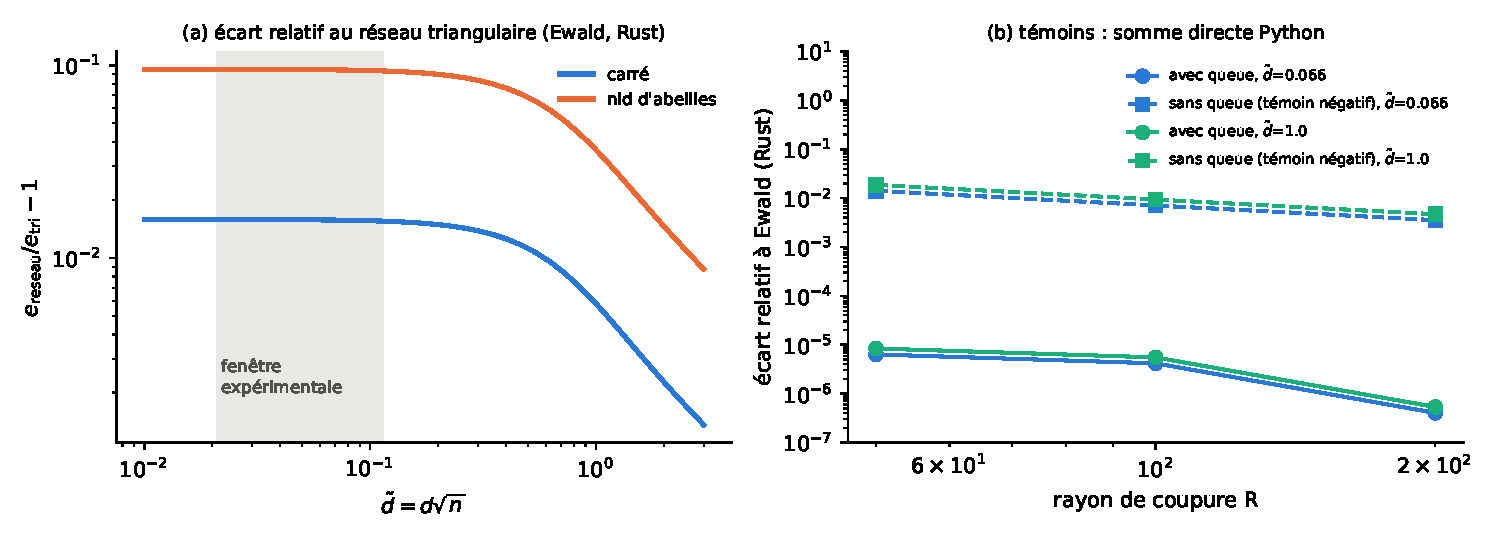
\includegraphics[width=\textwidth]{ch5_U1_dipolar.pdf}
\caption{U1 \tierX. (a) Écart relatif des réseaux carré et en nid d'abeilles au réseau triangulaire (énergies
d'Ewald exactes, rusty-SUNDIALS), en fonction de $\tilde d$. La bande grise est la fenêtre expérimentale déduite de
JARVIS-DFT. (b) Témoins : une somme directe en Python, \emph{avec} la queue uniforme exacte, converge vers la
valeur d'Ewald ; \emph{sans} la queue (témoin négatif), l'erreur reste de l'ordre de $10^{-2}$.}\label{ch5:fig:U1}
\end{figure}

\paragraph{Le résultat \tierX.} Sur toute la grille, les deux écarts restent positifs :
\begin{itemize}
\item $e_\mathrm{carre}/e_\mathrm{tri}-1$ décroît de $1{,}58\times10^{-2}$ à $1{,}36\times10^{-3}$ ;
\item l'écart du nid d'abeilles décroît de $9{,}53\times10^{-2}$ à $8{,}75\times10^{-3}$.
\end{itemize}
Converti en énergie (non écrantée, à diviser par $\varepsilon_r$), l'écart carré moins triangulaire vaut
$0{,}0014$, $0{,}044$ et $0{,}224$~meV par exciton aux trois densités. Ces valeurs sont interpolées sur la grille ;
l'article donnait $0{,}223$~meV au point de grille le plus proche. C'est de un à cinq ordres de grandeur sous la
profondeur des puits de moiré, \og des dizaines à 100~meV \fg{}~\cite{ch5:wang}. Dans l'étude publiée, aucun
des 21 compétiteurs relaxés par CVODE n'est passé sous le réseau triangulaire~\cite{ch2dip}.

\paragraph{Les témoins.}
\begin{itemize}
\item \emph{Positif.} Une somme directe Python indépendante, plus la queue exacte $2\pi/(\sqrt{R^2+\tilde
d^2}+R)$, retrouve la valeur d'Ewald de Rust. L'écart relatif est de $4{,}0\times10^{-7}$ à $\tilde d=0{,}066$ et
de $5{,}3\times10^{-7}$ à $\tilde d=1$, pour $R=200$. L'énergie d'Ewald ne dépend pas du paramètre de
découpage $\eta$ à mieux que $9{,}0\times10^{-15}$ près.
\item \emph{Négatif.} Sans la queue, la même somme se trompe de $3{,}5\times10^{-3}$ et $4{,}7\times10^{-3}$ à
$R=200$, et de $1{,}4\times10^{-2}$ à $R=50$.
\item \emph{Négatif.} Le script vérifie que $h_d(d^2)<0$ pour $d=0{,}5$, $1$ et $2$. Les réseaux carré et en nid
d'abeilles gardent une énergie plus haute en chacun des 41 points de la grille.
\end{itemize}
Nous avons aussi relancé, à part, deux relaxations de l'étude publiée à $\tilde d=0{,}066$ (commande
\texttt{dipolar\_crystal main <dossier> 0.066 1 0 1}, environ 8~minutes sur deux c\oe urs) :
\begin{itemize}
\item le départ uniforme \texttt{uniform\_00} finit à un écart relatif de $1{,}382373\times10^{-3}$, avec 4 défauts ;
\item la boîte incommensurable, témoin négatif, finit à $2{,}000407\times10^{-3}$, avec 8 défauts.
\end{itemize}
Ces deux valeurs sont celles de l'enregistrement, chiffre pour chiffre.

\paragraph{Ce que cela ne montre pas.}
\begin{itemize}
\item Le modèle est classique, à température nulle, avec des dipôles rigides et sans écrantage : pas de forme de
Rytova--Keldysh, pas de potentiel de moiré, pas d'énergie cinétique. Dans la fenêtre expérimentale, les vrais excitons
forment un gaz quantique, pas un cristal classique~\cite{ch5:wang}.
\item Le $d$ de JARVIS est un substitut : celui de deux empilements homogènes, et non celui d'une hétérobicouche. Le jeu
de données fixe l'échelle de $\tilde d$ ; il ne teste pas le théorème.
\item Aucune relaxation ne prouve l'optimalité : 21 essais ne couvrent pas l'infinité des configurations.
\end{itemize}

% =====================================================================================================
\section{U2 -- Cristaux de Yukawa plans : plasmas poussiéreux et colloïdes}\label{ch5:U2}

\paragraph{La question.} Dans un plasma poussiéreux de laboratoire, des micrograins chargés lévitent dans un plan.
Ils se repoussent par un potentiel coulombien écranté par les ions, $V(r)=Q^2e^{-r/\lambda_D}/r$. Des colloïdes
chargés en suspension se comportent de même. À densité fixée, quelle configuration minimise l'énergie ? On
observe des cristaux hexagonaux ; peut-on le démontrer dans ce modèle ?

\paragraph{Le théorème et son niveau.} Avec $t=r^2$ et $\kappa=\ell/\lambda_D$, où $\ell$ est la longueur
caractéristique de la densité, $g_\kappa(t)=e^{-\kappa\sqrt t}/\sqrt t$. La preuve humaine \tierC{} se fait en
trois étapes :
\begin{itemize}
\item $t\mapsto\sqrt t$ est une fonction de Bernstein et $x\mapsto e^{-\kappa x}$ est complètement monotone,
donc leur composée $e^{-\kappa\sqrt t}$ est complètement monotone (c'est la règle CM\,$\circ$\,Bernstein de la bibliothèque P3, doi:10.5281/zenodo.23653842) ;
\item $t^{-1/2}$ est complètement monotone ;
\item un produit de deux fonctions complètement monotones l'est encore (règle de Leibniz : chaque terme a le bon
signe).
\end{itemize}
Lean le vérifie \tierA{} (Lean 4.34.1), conditionnellement à l'amont :
\begin{leanbox}[: \texttt{formal\_cert/Autoresearch/Yukawa.lean} (énoncés)]
\begin{lstlisting}[language=Lean]
theorem yukawa_admissible {κ : ℝ} (hκ : 0 < κ) : AdmissiblePotential (g κ)
theorem triangular_yukawa_optimal {κ : ℝ} (hκ : 0 < κ) (C : Set Plane) (hC : LocallyFinite C)
    (hdens : DensityOne C) : latticeEnergy (g κ) ≤ energy (g κ) C
theorem latticeEnergy_yukawa_lt_top {κ : ℝ} (hκ : 0 < κ) : latticeEnergy (g κ) < ⊤
\end{lstlisting}
\end{leanbox}
Le module \texttt{YukawaMix.lean} étend le résultat à tout mélange fini $\sum_iw_ie^{-\kappa_ir}/r$ à poids
$w_i\ge0$. Le témoin négatif formel est le mélange signé $g_1-2g_2$ : il vaut $2e^{-1/2}-4e^{-1}\approx-0{,}2585$
en $t=\tfrac14$, donc il n'est pas admissible. Le théorème ne s'applique pas à lui, ce qui ne veut pas dire que
l'optimalité échoue. Article : doi:10.5281/zenodo.23646105~\cite{ch2yuk}.

\paragraph{Les données.} Le 2026-10-25, une recherche sur le Hub (\emph{dusty plasma}, \emph{complex plasma},
\emph{colloid}, \emph{yukawa}, \emph{wigner crystal}) n'a trouvé aucun jeu de positions de grains ou de
colloïdes~\cite{ch2yuk}. C'est une absence constatée par recherche, pas une preuve. Les conditions initiales
désordonnées viennent donc d'un tout autre domaine, la catalyse :
\begin{itemize}
\item identifiant \texttt{colabfit/OC20\_IS2RES\_val\_id}, licence CC-BY-4.0~\cite{ch5:oc20} ;
\item fichier \texttt{co/co\_10.parquet}, 142\,986\,687 octets ; son sha256 local est égal au hash LFS du Hub à la
révision \texttt{6a1dfef12aec878b4cda99edd54b16a6a254e135} ;
\item des structures d'adsorbats, tournées en 3D, projetées sur le plan, remises à l'échelle et filtrées par une
distance minimale.
\end{itemize}
Le script vérifie le sha256 et retrouve dans le fichier les identifiants de configuration OC20 listés dans
\texttt{provenance.json}. Ces données fournissent un \emph{désordre} d'aspect réaliste, rien de plus : des molécules
adsorbées sur un catalyseur n'ont rien à voir avec des grains chargés écrantés.

\paragraph{La méthode numérique.} Le module \texttt{exact.rs} de \texttt{qf-yukawa-crystal} a trois parties :
\begin{itemize}
\item des sommes de réseau du potentiel \emph{non tronqué}, avec une borne rigoureuse de la queue ;
\item une décomposition d'Ewald indépendante ;
\item une boîte périodique sommant toutes les images dans le rayon $R$, avec énergie, force et hessienne
analytiques.
\end{itemize}
La borne de queue repose sur les cellules de Voronoï : pour $V$ décroissant, la queue au-delà de $R$ vaut au plus
$(\pi/A)\bigl(1+\delta/(R-2\delta)\bigr)e^{-\kappa(R-2\delta)}/\kappa$. La relaxation (\texttt{exact-relax}) utilise
CVODE : BDF, jacobien égal à l'opposé de la hessienne, $\mathrm{rtol}=10^{-10}$, $\mathrm{atol}=10^{-12}$ et
tolérance de force $10^{-9}$. Chaque minimum est contrôlé par le spectre de la hessienne. Ce calcul corrige un
erratum publié : une version antérieure tronquait le potentiel à $r_c=8$ avec un décalage de force, et ce potentiel
tronqué n'est plus complètement monotone.

\paragraph{Le script.} \texttt{code/ch5\_U2\_yukawa.py SORTIE} :
\begin{enumerate}
\item il copie les conditions initiales dans une crate de travail ;
\item il lance \texttt{yukawa\_crystal exact-refs}, puis \texttt{exact-relax 2 1 0 0}. À $\kappa=2$, cela fait
trois relaxations d'environ 1 à 2~minutes chacune sur deux c\oe urs : un départ OC20, un départ uniforme et une
boîte incommensurable ;
\item il exécute les témoins et trace \texttt{figures/ch5\_U2\_yukawa.pdf}.
\end{enumerate}
L'option \texttt{--skip-relax} relit l'enregistrement au lieu de relancer les relaxations.

\begin{figure}[ht]\centering
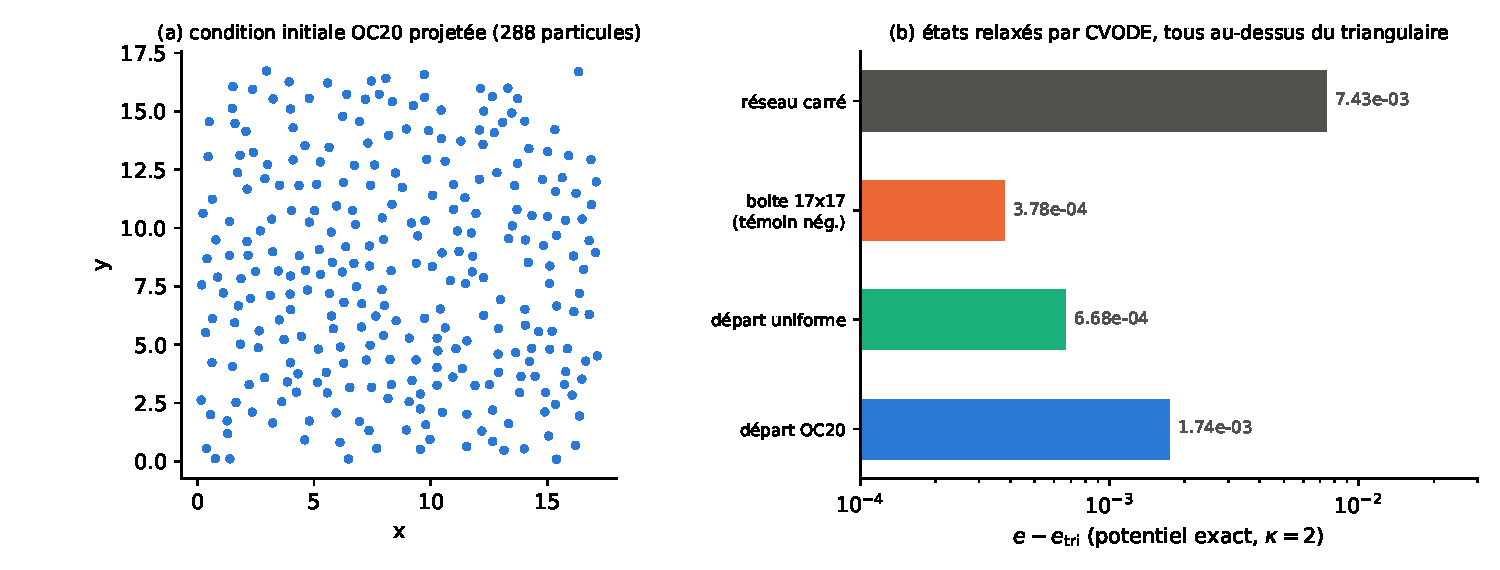
\includegraphics[width=\textwidth]{ch5_U2_yukawa.pdf}
\caption{U2 \tierX. (a) Condition initiale tirée d'OC20 (288 particules dans une boîte qui contient exactement le
réseau triangulaire). (b) Écart $e-e_\mathrm{tri}$ des états relaxés par CVODE sous le potentiel exact
($\kappa=2$), à comparer à l'écart du réseau carré. Aucun état n'est en dessous du réseau
triangulaire.}\label{ch5:fig:U2}
\end{figure}

\paragraph{Le résultat \tierX.} Énergies par particule à densité un, en convention $\tfrac12\sum$ :

\begin{center}\small
\begin{tabular}{lllll}\toprule
$\kappa$ & triangulaire (exact) & carré (exact) & écart & tronqué--exact (tri.)\\\midrule
1 & 1,6253213396063 & 1,6348554953172 & $9{,}534\times10^{-3}$ & $-1{,}771\times10^{-2}$\\
2 & 0,3935428489324 & 0,4009742487651 & $7{,}431\times10^{-3}$ & $-9{,}48\times10^{-6}$\\
\bottomrule\end{tabular}
\end{center}
La borne de queue vaut au plus $5{,}6\times10^{-17}$ ($\kappa=1$, $R=40$) et $1{,}2\times10^{-16}$ ($\kappa=2$,
$R=20$). Les trois relaxations à $\kappa=2$ convergent, sans mode négatif de la hessienne :
\begin{itemize}
\item départ OC20 : écart $1{,}742\times10^{-3}$, 24 défauts, 157 pas de CVODE ;
\item départ uniforme : écart $6{,}68\times10^{-4}$, 4 défauts ;
\item boîte incommensurable $17\times17$ : écart $3{,}78\times10^{-4}$, 4 défauts.
\end{itemize}
Dans l'étude complète, aucune des 24 étapes relaxées sous le potentiel exact n'est passée sous le réseau
triangulaire~\cite{ch2yuk}.

\paragraph{Les témoins.}
\begin{itemize}
\item \emph{Positifs.} Une somme directe Python du réseau retrouve les valeurs exactes de Rust à
$1{,}4\times10^{-16}$ près en relatif au plus (le seuil exigé est $10^{-12}$). Par ailleurs, la boîte périodique contenant le réseau parfait égale la somme
infinie à $2{,}2\times10^{-16}$ près.
\item \emph{Négatifs.} Les énergies tronquées à $r_c=8$ ratent la valeur exacte de bien plus que $10^{-9}$. La boîte
$17\times17$, qui ne peut pas contenir le réseau triangulaire, reste au-dessus. Le réseau carré parfait est un col
du potentiel exact, avec 72 modes négatifs à $\kappa=2$ et 64 à $\kappa=1$~\cite{ch2yuk}.
\end{itemize}

\paragraph{Ce que cela ne montre pas.}
\begin{itemize}
\item Les données OC20 ne contiennent aucune physique des plasmas : elles servent seulement de désordre initial.
\item Le potentiel $K_0(\kappa r)$, la fonction de Green de Debye--Hückel en 2D, n'est pas traité. Les mélanges à poids
négatifs, la température finie et l'unicité ne le sont pas non plus.
\item Le recuit n'a pas été refait avec le potentiel exact.
\end{itemize}

% =====================================================================================================
\section[U3 -- Hélium superfluide et test de Feynman--Bijl]{U3 -- Hélium superfluide : facteur de structure et test de Feynman--Bijl}\label{ch5:U3}

\paragraph{La question.} La diffraction de rayons X ou de neutrons mesure le facteur de structure statique $S(k)$
d'un liquide. Pour un gaz de Bose faiblement interagissant, la théorie de Bogoliubov prédit
$S_B(k)=\varepsilon_0(k)/\varepsilon_B(k)$, avec $\varepsilon_0=\hbar^2k^2/2m$. Peut-on dire, \emph{à partir de
$S(k)$ seul}, que l'hélium~4 superfluide n'est pas un gaz de Bogoliubov ?

\paragraph{Le théorème et son niveau.} Posons $k^*=2mc/\hbar$, où $c$ est la vitesse du son. On a alors
$S_B(k)=k/\sqrt{k^{*2}+k^2}$ et
\[S_B(k)\le\sqrt{\frac{k}{2k^*}},\qquad\text{avec égalité si et seulement si }k=k^* .\]
\begin{humanproof}
Les deux membres sont positifs ; on compare leurs carrés. $S_B^2\le k/2k^*$ équivaut à
$2k^*k\le k^{*2}+k^2$, c'est-à-dire à $(k-k^*)^2\ge0$.
\end{humanproof}
L'énoncé est de niveau \tierAs{}, dans l'environnement QuantumFluids (Lean v4.34.0-rc2 ; aucun rejeu \texttt{leanchecker} enregistré pour cet environnement), sous le nom
\lean{sBog_le_sqrt}. Les deux témoins sont vérifiés par le noyau : le test se déclenche sur la valeur libre $S=1$
pour tout $0<k<2k^*$ (\lean{free_S_one_violates}), et ne se déclenche jamais sur $S_B$. Le corollaire
\lean{not_bogoliubov_of_structure_factor} donne le \og test de diffraction \fg{} : si un $S$ mesuré dépasse
$\sqrt{k/2k^*}$, ce $S$ n'est pas le facteur de structure d'un gaz de Bogoliubov ayant cette vitesse du son.
L'argument de Feynman--Bijl relie $S$ à l'énergie d'excitation, $\varepsilon(k)\le\hbar^2k^2/(2mS(k))$. Son
c\oe ur à un mode est formalisé en Lean 4.34.1, l'identité de la règle de somme f étant prise comme
\emph{hypothèse}. Articles : doi:10.5281/zenodo.23646117~\cite{ch3-bsk} et
doi:10.5281/zenodo.23653846~\cite{ch3-fb}.

\paragraph{Les données (pas Hugging Face).} Aucun jeu de données de facteur de structure n'existe sur le Hub : les
recherches de ces deux articles n'en ont trouvé aucun. Nous utilisons la Table~14.1 de la compilation de Donnelly et
Barenghi~\cite{ch3-db}, dans son édition web (supposée, sans vérification, reproduire la table de 1998) :
\begin{itemize}
\item 99 points avec $Q>0$ : 49 points de rayons X (Robkoff--Hallock) et 50 points de neutrons (Svensson et al.) ;
\item des températures de 1,4 à 4~K, aucune barre d'erreur imprimée.
\end{itemize}
C'est une source secondaire de niveau \tierL{}. Le fichier extrait est
\url{papers/prog_superfluid_structure_factor/data/he4_Sk_donnelly_table14_1.csv}. On prend
$c=238{,}3\pm0{,}1$~m/s~\cite{ch3-godfrin}, d'où $k^*=3{,}00379$~\AA$^{-1}$ (entre 3,0025 et 3,0051).

\paragraph{La méthode.} Pour chaque point, le verdict est :
\begin{itemize}
\item \textsc{compatible} si $S\le\sqrt{Q/2k^*}$ ;
\item \textsc{réfuté} si $S-\sqrt{Q/2k^*}>\Delta$ ;
\item \textsc{indécis} sinon.
\end{itemize}
Le seuil $\Delta=0{,}082$ est l'écart entre les maxima des deux jeux de la table. Ce seuil a été fixé après coup, il
n'était pas préenregistré. Côté rusty-SUNDIALS, le module \texttt{linear\_response} de \texttt{qf-gpe2d} donne une
contre-épreuve : on excite le fondamental de Gross--Pitaevskii (grille $32\times32$, pas fractionnaire de Strang),
on mesure la fréquence de la réponse, et l'on en tire $\varepsilon_B(k)$ et $S(k)$.

\paragraph{Le script.} \texttt{code/ch5\_U3\_helium.py SORTIE [--gpe-json FICHIER]} applique le test et exécute les
témoins. Si on lui donne la sortie de l'exemple \texttt{bogoliubov\_dispersion} de \texttt{qf-gpe2d}, il trace aussi
la réponse linéaire.

\begin{figure}[ht]\centering
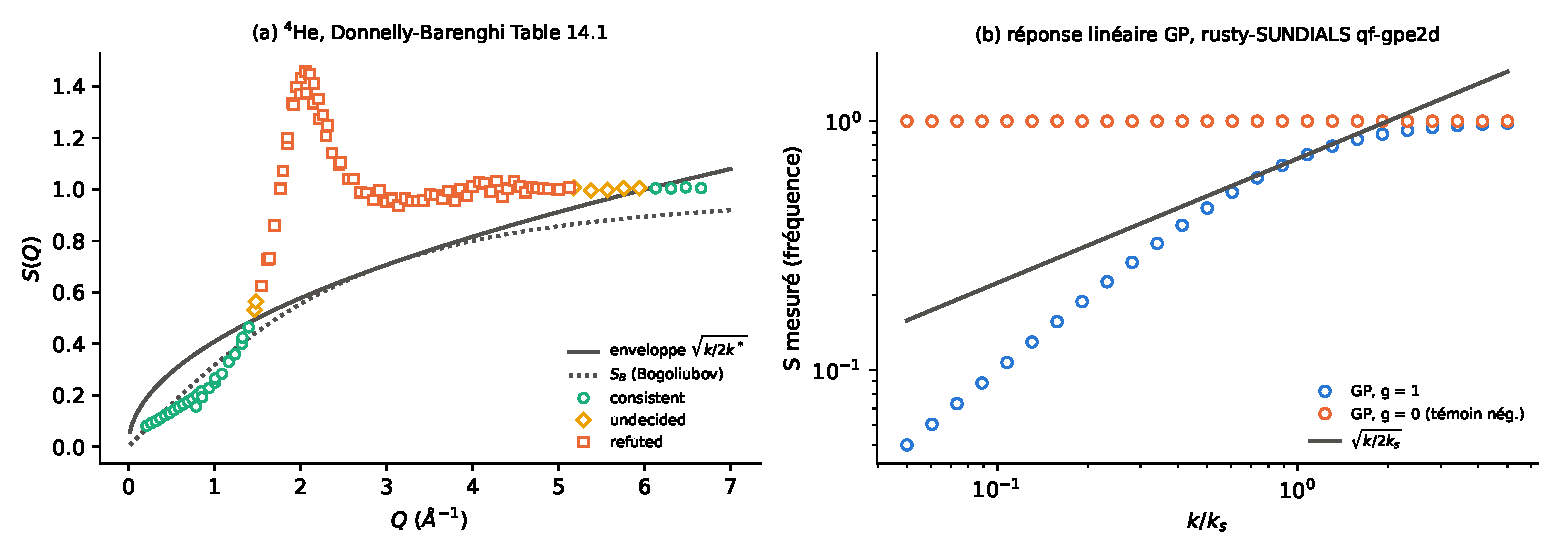
\includegraphics[width=\textwidth]{ch5_U3_helium.pdf}
\caption{U3. (a) $S(Q)$ de l'hélium~4 (Table~14.1, niveau~L) face à l'enveloppe $\sqrt{Q/2k^*}$ (trait plein) et à
$S_B$ (pointillé) ; la couleur donne le verdict (arithmétique, niveau~X). (b) Réponse linéaire de Gross--Pitaevskii
calculée par rusty-SUNDIALS \tierX{} : $S$ mesuré pour $g=1$ sous l'enveloppe, témoin $g=0$ ($S=1$) au-dessus pour
$k<2k_s$.}\label{ch5:fig:U3}
\end{figure}

\paragraph{Le résultat.} Sur les 99 points, 29 sont compatibles, 7 indécis et 63 réfutés. Les 21 points de la région
du pic et du roton ($1{,}7\le Q\le2{,}4$~\AA$^{-1}$) sont tous réfutés : $S$ y dépasse l'enveloppe d'un facteur
1,62 à 2,49. Les mesures de l'hélium~4 ne sont donc pas le $S$ d'un gaz de Bogoliubov de même vitesse du son. Ce
résultat de manuel est désormais une conséquence d'un énoncé vérifié et d'une table publiée.

Nous avons relancé l'exemple \texttt{bogoliubov\_dispersion} (10~min 24~s sur un c\oe ur), et sa sortie est
identique bit à bit à l'enregistrement. Dans cette réponse linéaire de Gross--Pitaevskii \tierX{} :
\begin{itemize}
\item la fréquence mesurée pour $g=1$ retrouve $\varepsilon_B$ à $4{,}1\times10^{-5}$ près en relatif ;
\item le $S$ mesuré reste sous l'enveloppe, puisque $\max(S/\sqrt{k/2k_s})-1=-1{,}4\times10^{-3}$ ;
\item le témoin $g=0$, un gaz libre où $S=1$, dépasse l'enveloppe aux 20 nombres d'onde du balayage tels que
$k<2k_s$.
\end{itemize}

\paragraph{Les témoins.}
\begin{itemize}
\item \emph{Positif.} $S_B$ ne déclenche le test en aucun des 99 points.
\item \emph{Négatif.} La valeur libre $S=1$ le déclenche en 95 points sur 95 avec $Q<2k^*$.
\end{itemize}
Les deux témoins sont aussi des théorèmes Lean.

\paragraph{Ce que cela ne montre pas.}
\begin{itemize}
\item La conclusion physique est conditionnelle \tierC{} : la table a été mesurée entre 1,4 et 4~K, et non à
$T=0$. Nous n'avons pas quantifié la variation du pic de $S$ avec la température.
\item Un point compatible n'est pas \emph{confirmé} \og Bogoliubov \fg{} : l'enveloppe n'est qu'une borne
supérieure, et aux petits $k$ elle a très peu de pouvoir de test.
\item Au-delà du pic, l'échec ressemble à celui du témoin $S=1$ : ce n'est plus la physique du roton.
\end{itemize}

% =====================================================================================================
\section[U4 -- Turbulence : borne d'enstrophie]{U4 -- Turbulence : borne d'enstrophie dans le modèle en couches \texorpdfstring{$\sigma=3$}{sigma=3}}\label{ch5:U4}

\paragraph{La question.} Les modèles en couches remplacent un champ de vitesse turbulent par une amplitude complexe
$v_n$ par octave de nombres d'onde, $k_n=2^n$, $n=0,\dots,N+1$. Les couches voisines échangent de l'énergie par un
terme quadratique. Ajoutons un terme dispersif $-i\omega_nv_n$ avec $\omega_n=Dk_n^3$ (\og $\sigma=3$ \fg). Peut-on
borner l'enstrophie $\Omega=\tfrac12\sum k_n^2|v_n|^2$, qui mesure les petites échelles, le long de \emph{toute}
trajectoire et pour \emph{toute} troncature $N$ ?

\paragraph{Le théorème et son niveau.} Le modèle conserve deux quantités :
\begin{itemize}
\item la \og masse \fg{} $S=\sum|v_n|^2=2E$ ;
\item l'invariant $H=\sum2^{-n}\omega_n|v_n|^2+\sum2^{-n}k_n\,\mathrm{Im}(\bar v_n^{\,2}v_{n+1})$, pour \emph{toute}
loi de dispersion réelle.
\end{itemize}
Pour $\omega_n=Dk_n^3$, la partie quadratique de $H$ vaut exactement $2D\Omega$. La partie cubique $C$ vérifie
$|C|\le S^{3/2}$.
\begin{humanproof}
Notons $H_3(0)$ la valeur de $H$ à l'instant $0$. Comme $H$ est conservé, $2D\Omega(t)=H_3(0)-C(t)$. Donc
$2D\Omega(t)\le H_3(0)+|C(t)|\le H_3(0)+S(t)^{3/2}$. Comme $S$ est conservé,
$2D\Omega(t)\le H_3(0)+(2E(0))^{3/2}$.
\end{humanproof}
Lean vérifie tout cela \tierAs{} (Lean v4.34.0-rc2, Mathlib du projet ; sans rejeu \texttt{leanchecker}) :
\begin{itemize}
\item l'identité de taux de $H$ le long du champ de vecteurs ;
\item la règle de dérivation en chaîne ;
\item la constance de $H$ et de $S$ sur $[0,T]$ ;
\item la borne \lean{enstrophy_bound_along_flow}, pour toute trajectoire sur $[0,T]$ et tout $N$.
\end{itemize}
L'énoncé suppose que la trajectoire existe et qu'elle est dérivable en chaque instant de $[0,T]$ : l'existence est
une \emph{hypothèse}, pas un théorème. Le niveau $N$ reste fixé. Article : doi:10.5281/zenodo.23646111~\cite{ch5:sigma3}.
\paragraph{Les données.} The Well~\cite{ch5:thewell} contient des simulations de fluides de grande taille. Nous
utilisons :
\begin{itemize}
\item identifiant : \url{polymathic-ai/turbulent_radiative_layer_2D} ;
\item révision \texttt{2ee7756575ff6f90981d0308cbcb6a2ab5995bdc}, licence CC-BY-4.0 selon la carte ;
\item le fichier\\ \url{data/test/turbulent_radiative_layer_tcool_0.32.hdf5},\\ sha256 \texttt{06cbd36c\dots f747},
vérifié par le script.
\end{itemize}
Ce sont des simulations Athena++ de l'équation d'Euler compressible 2D avec refroidissement radiatif.

Le spectre est construit ainsi, pour quatre instantanés développés (indices 25, 50, 75 et 100) :
\begin{enumerate}
\item on prend la FFT de la vitesse selon l'axe périodique $x$, sans le mode $k_x=0$ ;
\item on fait la moyenne en $y$ ;
\item on somme $k_x\in[2^n,2^{n+1})$ dans la couche $n=0,\dots,5$.
\end{enumerate}
Cette étape lit le HDF5 avec \texttt{h5py}, absent de l'environnement \texttt{.venv} d'AutoevolveAI : le script
relit donc le fichier \texttt{well\_amps.txt} que ces étapes ont produit. Les pentes de $\log_2$ des spectres valent
$-2{,}13$, $-1{,}56$, $-1{,}79$ et $-1{,}81$~\cite{ch5:sigma3}.

\paragraph{La méthode numérique.} Le module \texttt{sigma.rs} de \texttt{qf-shell-cascade} intègre le modèle avec CVODE :
\begin{itemize}
\item BDF, jacobien analytique, $\mathrm{atol}=10^{-3}\,\mathrm{rtol}$, $D=0{,}05$ ;
\item suprema pris aux points de pas internes de CVODE, sans interpolation.
\end{itemize}
Le programme \texttt{sigma3\_study full} enchaîne cinq blocs :
\begin{itemize}
\item un témoin positif, la convergence de la conservation avec la tolérance ;
\item un témoin négatif, un couplage perturbé ;
\item un balayage de troncatures $n_{\max}\le7$ ;
\item la comparaison $\sigma=2$ contre $\sigma=3$ sur des données concentrées dans la dernière couche ;
\item 24 trajectoires initialisées par les modules de The Well, avec deux tirages de phases aléatoires et
$n_{\max}=5,6,7$.
\end{itemize}

\paragraph{Le script.} \texttt{code/ch5\_U4\_shell.py SORTIE} lance \texttt{sigma3\_study full} (de 2,5 à 6~minutes
selon la charge de la machine), vérifie les critères et trace \texttt{figures/ch5\_U4\_shell.pdf}.

\begin{figure}[ht]\centering
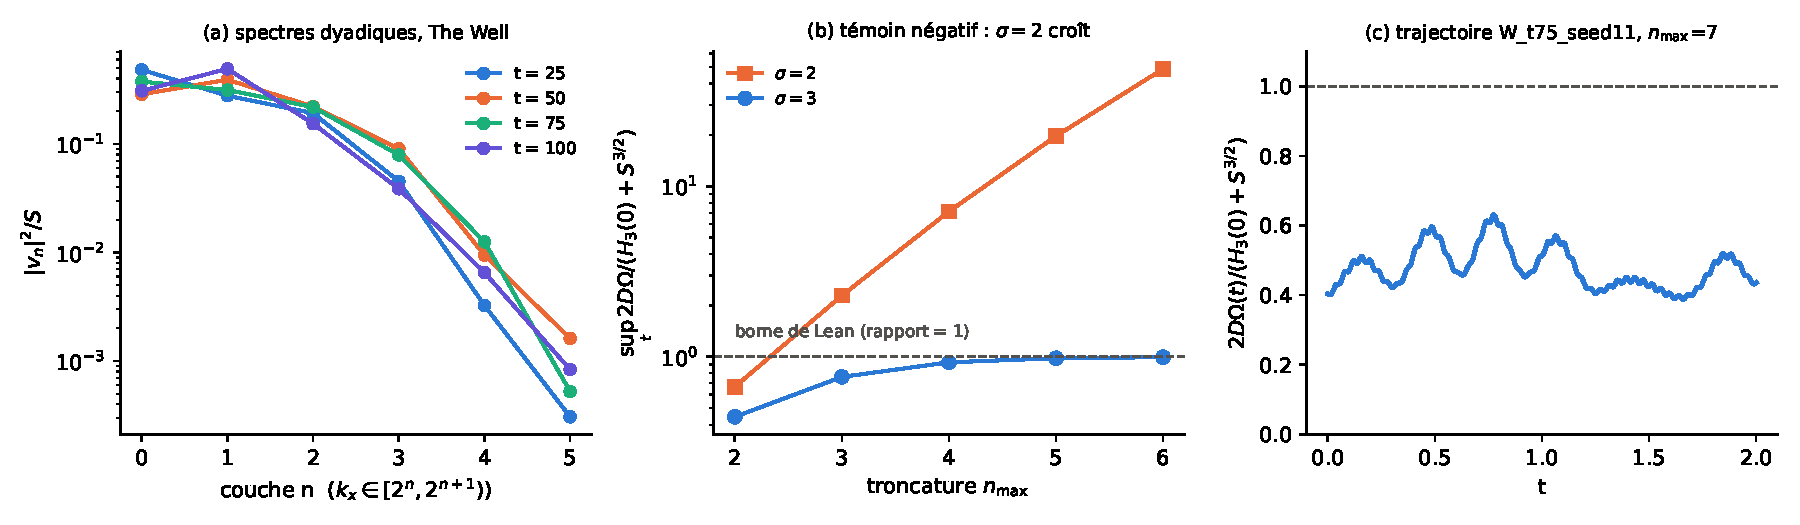
\includegraphics[width=\textwidth]{ch5_U4_shell.pdf}
\caption{U4 \tierX. (a) Spectres dyadiques de quatre instantanés de The Well, normalisés à $S=1$. (b) Rapport
$\sup_t2D\Omega/(H_3(0)+S^{3/2})$ sur des données concentrées dans la dernière couche : il reste sous 1 pour
$\sigma=3$ et croît avec $n_{\max}$ pour $\sigma=2$ (témoin négatif). (c) Le rapport le long de la trajectoire
initialisée par The Well qui s'approche le plus de la borne.}\label{ch5:fig:U4}
\end{figure}

\paragraph{Le résultat \tierX.} Les 17 trajectoires $\sigma=3$ du balayage et de la comparaison restent toutes sous la
borne. Le rapport $\sup_t2D\Omega(t)/(H_3(0)+S(0)^{3/2})$ vaut au plus 0,995 ; ce maximum est atteint sur des données
concentrées dans la dernière couche, où le rapport tend vers 1 quand $n_{\max}$ croît (0,444, 0,762, 0,928, 0,981
et 0,995 pour $n_{\max}=2,\dots,6$). Les 24 trajectoires initialisées par The Well restent aussi sous la borne, avec
un rapport d'au plus 0,631. Leurs dérives relatives sont au plus $2{,}4\times10^{-8}$ sur $S$ et $1{,}2\times10^{-6}$
sur $H$. Le fichier \texttt{sigma3\_study.json} recalculé est identique à l'enregistrement de
l'article~\cite{ch5:sigma3}, aux temps d'exécution près.

\paragraph{Les témoins.}
\begin{itemize}
\item \emph{Positif.} Avec le vrai couplage, la dérive de $H$ diminue avec la tolérance. Pour $n_{\max}=4$, elle
vaut $2{,}6\times10^{-5}$, $8{,}6\times10^{-7}$ puis $1{,}9\times10^{-8}$ pour
$\mathrm{rtol}=10^{-6},10^{-8},10^{-10}$.
\item \emph{Négatif.} Si l'on perturbe le couplage sortant de la couche~1 de $10^{-2}$, la dérive de $H$ reste
bloquée vers $2{,}3\times10^{-3}$ ($n_{\max}=4$) et $5{,}4\times10^{-3}$ ($n_{\max}=6$), quelle que soit la
tolérance. La conservation vient donc de la structure du modèle, pas de la précision du solveur.
\item \emph{Négatif.} Pour $\sigma=2$, la même inégalité n'a pas de démonstration, et le rapport vaut 0,667, 2,29,
7,11, 19,7 puis 48,8 pour $n_{\max}=2,\dots,6$. Il dépasse 1 dès $n_{\max}=3$ et croît plus vite qu'une
exponentielle de raison 2 sur cette plage (figure~\ref{ch5:fig:U4}b).
\end{itemize}

\paragraph{Ce que cela ne montre pas.}
\begin{itemize}
\item Les données de The Well donnent une forme de spectre réaliste, et rien d'autre. L'écoulement est compressible
et refroidi, il ne conserve pas l'énergie. Le spectre est unidimensionnel et ne porte pas de phases (elles sont
tirées au hasard).
\item Sur $T=2$, les couches supérieures, initialement vides, se remplissent à peine. Ces trajectoires ne sondent donc
pas la dépendance en $N$.
\item Il n'y a aucun énoncé en nombre infini de couches. L'uniformité en $N$ demande des données initiales dont
$\Omega(0)$ et $S(0)$ sont bornés uniformément en $N$ (corollaire de niveau C).
\item L'amortissement de BDF fait dériver $S$ vers le bas. Les marges observées dépassent largement ces dérives,
mais la simulation ne remplace pas le théorème.
\end{itemize}

% =====================================================================================================
\section{U5 -- Génétique : fixation d'une mutation}\label{ch5:U5}

\paragraph{La question.} Une population compte $N$ individus, dont $i$ portent une mutation de valeur sélective
relative $r$. Quelle est la probabilité que la mutation finisse par envahir toute la population (la
\emph{fixation}) ? Et que devient cette probabilité quand la population vit sur un graphe ?

\paragraph{Le modèle de Moran.} À chaque pas, un individu est choisi pour se reproduire avec une probabilité
proportionnelle à sa valeur sélective, et un individu tiré uniformément meurt. Le nombre de mutants est une chaîne de
naissance et de mort sur $\{0,\dots,N\}$. Ses probabilités de montée et de descente sont
\[p_i=\frac{ri}{ri+N-i}\cdot\frac{N-i}{N},\qquad q_i=\frac{N-i}{ri+N-i}\cdot\frac iN,\qquad\text{donc } p_i=r\,q_i .\]

\paragraph{Le théorème et son niveau.} Notons $\varphi_i$ la probabilité de fixation partant de $i$ mutants. L'équation
du premier pas donne $p_i(\varphi_{i+1}-\varphi_i)=q_i(\varphi_i-\varphi_{i-1})$, avec $\varphi_0=0$ et
$\varphi_N=1$.
\begin{humanproof}[Démonstration humaine (formule)]
Posons $\delta_i=\varphi_{i+1}-\varphi_i$. L'équation donne $\delta_i=\delta_{i-1}/r$, donc $\delta_i=r^{-i}\delta_0$
et $\varphi_i=\delta_0S_i$, où $S_i=\sum_{k<i}r^{-k}$. La condition $\varphi_N=1$ fixe
$\delta_0=1/S_N$. Pour $r\ne1$, on obtient
\[\varphi_i=\frac{S_i}{S_N}=\frac{1-r^{-i}}{1-r^{-N}} .\]
Pour $r=1$, on obtient $\varphi_i=i/N$.
\end{humanproof}
Le programme P7 vérifie davantage \tierA{} (Lean 4.34.1). Il montre la \emph{limite d'absorption},
$P^n(i,N)\to(1-r^{-i})/(1-r^{-N})$, et l'unicité : toute fonction harmonique à l'intérieur avec les valeurs $0$ et
$1$ au bord est $\varphi$. Le programme N4 démontre le théorème isotherme (naissance--mort) : sur un graphe
fortement connexe dont la matrice de remplacement est doublement stochastique, la fixation suit la même loi.
\begin{leanbox}[: \texttt{PopGen/MoranFixation.lean} et \texttt{EvoGraph/BirthDeath.lean} (énoncés)]
\begin{lstlisting}[language=Lean]
theorem moran_fixation_limit_closed {N : ℕ} {r : ℝ} (hN : 0 < N) (hr : 0 < r) (hr1 : r ≠ 1)
    (i : Fin (N + 1)) :
    Tendsto (fun n => kPow (moranP N r) n i (Fin.last N)) atTop
      (𝓝 ((1 - r⁻¹ ^ (i : ℕ)) / (1 - r⁻¹ ^ N)))
theorem moran_fixation_unique {N : ℕ} {r : ℝ} (hN : 0 < N) (hr : 0 < r) {g : Fin (N + 1) → ℝ}
    (hg : InteriorHarmonic (moranP N r) g) (g0 : g 0 = 0) (g1 : g (Fin.last N) = 1) :
    ∀ i, g i = moranFix N r i
theorem isothermal_fixation {W : Fin n → Fin n → ℝ} {r : ℝ} (hn : 0 < n) (hr : 0 < r)
    (hW : Isothermal W) (hsc : StronglyConnected W) (S : Finset (Fin n)) :
    Tendsto (fun t => sPow (bdK (fun _ => 1) W r) t S univ) atTop (𝓝 (moranFix n r S.card))
\end{lstlisting}
\end{leanbox}
Le théorème général d'absorption de P7 et la version à un seul mutant du théorème isotherme réapparaissent sous
les noms \lean{KAL} et \lean{ILENE} dans la section~\ref{ch5:acronymes}.

Le nombre de mutants sur un graphe n'est \emph{pas} une chaîne de Markov en général. Sur le 4-cycle, la probabilité de
montée d'un pas dépend de la configuration, $1/3$ contre $2/3$ à $r=2$. Ce qui est vrai, et prouvé, c'est le biais
\emph{par configuration} $P^+=r\,P^-$. Sur l'étoile à $n=3$ nœuds, qui n'est pas isotherme, les limites valent
$5/12$, $2/3$ et $7/12$, contre $4/7$ pour Moran. Articles : doi:10.5281/zenodo.23653850~\cite{ch4:P7} et
doi:10.5281/zenodo.23660071~\cite{ch4:N4}.

\paragraph{Les données : ce qu'elles illustrent, et ce qu'elles n'estiment pas.} Le dépôt Genetic de l'auteur
utilise les jeux \texttt{katarinagresova/Genomic\_Benchmarks\_*}~\cite{ch5:gb}. Nous en prenons un :
\begin{itemize}
\item identifiant \url{katarinagresova/Genomic_Benchmarks_demo_coding_vs_intergenomic_seqs}, révision
\texttt{85458172cab6cffad46cb172e64ca94780506ed6} ;
\item la partie test, \url{data/test-00000-of-00001-6fccc31405110e30.parquet}, 2\,456\,511 octets, sha256
\texttt{dfe13715\dots 9afe}.
\end{itemize}
La carte n'indique \emph{aucune} licence et ne dit pas ce que signifient les étiquettes 0 et 1. Nous ne
reproduisons que des statistiques agrégées, et la licence du paquet amont n'a pas été vérifiée.

Le script compte 25\,000 séquences, 12\,500 par étiquette, toutes de longueur 200, sans autre symbole que A, C, G et T.
La fraction de GC vaut 0,5381 pour l'étiquette~0 et 0,4004 pour l'étiquette~1 (figure~\ref{ch5:fig:U5}c).

C'est ce à quoi ressemble une donnée de séquence : une mutation ponctuelle y est le remplacement d'une lettre.
\textbf{Mais ce jeu n'estime aucune valeur sélective $r$}, et rien dans ce chapitre n'en tire une. Les valeurs de $r$
utilisées plus bas (0,8, 1, 1,2, 1,5 et 2) sont \emph{choisies}, pas mesurées.

\paragraph{La méthode numérique.} La crate \texttt{qf-popgen} écrit la chaîne absorbante comme une équation
différentielle linéaire, $\dot\pi=\pi(P-I)$ : c'est l'équation de Kolmogorov progressive de la chaîne uniformisée. Elle
l'intègre avec CVODE (BDF, jacobien exact, $\mathrm{rtol}=10^{-11}$, $\mathrm{atol}=10^{-15}$). Un
\emph{certificat d'absorption} refuse toute exécution douteuse, dans l'esprit « fail-closed » (qui refuse par défaut) : une exécution n'est
acceptée que si cinq conditions sont réunies :
\begin{itemize}
\item le noyau est stochastique et absorbant ;
\item la masse totale est conservée ;
\item aucune composante ne devient négative ;
\item la masse intérieure est tombée sous $10^{-9}$ ;
\item la masse en $N$ égale la cible à $10^{-8}$ près.
\end{itemize}
Le passage de l'équation différentielle au noyau à $n$ pas (un mélange de Poisson) n'est pas formalisé.

Enfin, \textbf{LeanFlow} certifie un nombre calculé. Sa fonction \texttt{lean.certify} accepte une affirmation sur des
encadrements rationnels et la traduit en un énoncé sur les entiers. La tactique \texttt{decide\_kernel}
(\lean{decide +kernel}) fait décider cet énoncé par le noyau, sans axiome supplémentaire. LeanFlow audite ensuite
\texttt{\#print axioms}, et un oracle exact en Python doit rendre le même verdict.

\paragraph{Le script.} \texttt{code/ch5\_U5\_fixation.py SORTIE} :
\begin{enumerate}
\item il télécharge le fichier à la révision épinglée, en vérifie l'empreinte et en tire les statistiques ;
\item il lance \texttt{fixation\_ode} ;
\item il compare les valeurs de CVODE aux fractions exactes ;
\item il soumet cinq affirmations à LeanFlow (Lean 4.34.1, cœur seul) ;
\item il trace \texttt{figures/ch5\_U5\_fixation.pdf}.
\end{enumerate}
Il dure une vingtaine de secondes.

\begin{figure}[ht]\centering
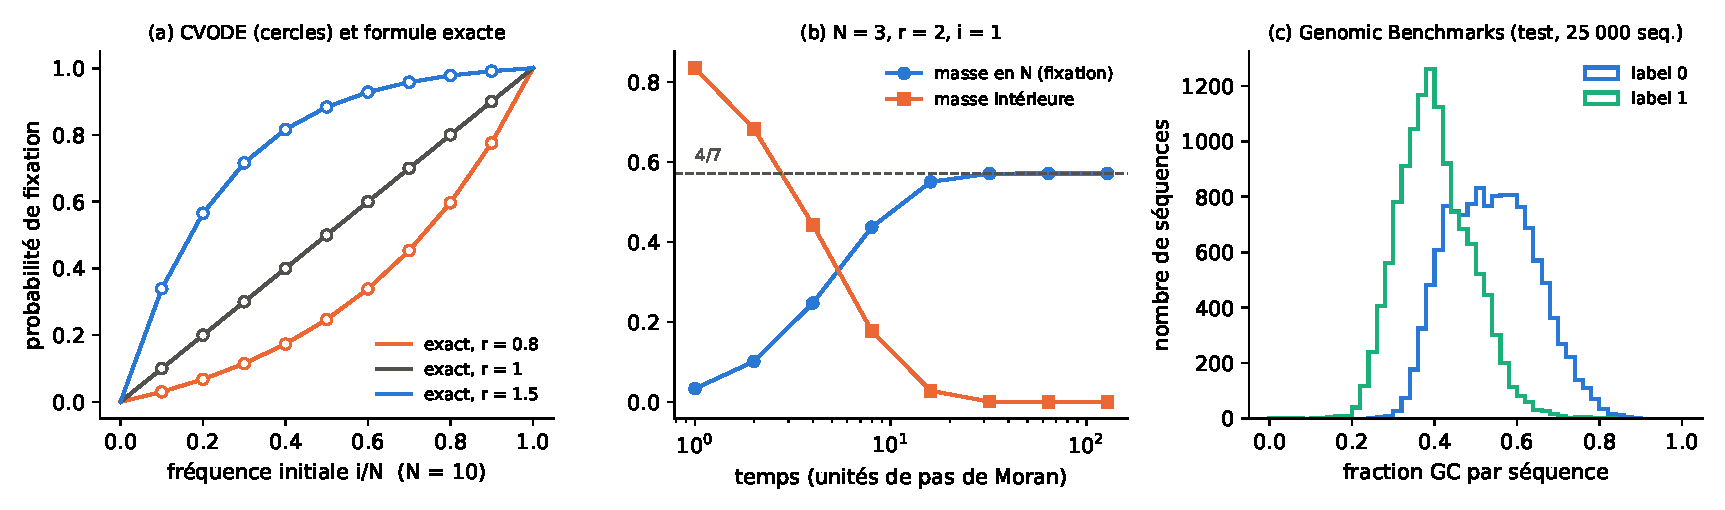
\includegraphics[width=\textwidth]{ch5_U5_fixation.pdf}
\caption{U5. (a) Probabilité de fixation pour $N=10$ : CVODE (cercles, \tierX) et formule exacte (traits), pour
$r=0{,}8$, $1$ et $1{,}5$. (b) Trajectoire de CVODE pour $N=3$, $r=2$, $i=1$ : la masse absorbée en $N$ tend vers
$4/7$, la masse intérieure s'éteint. (c) Fraction de GC des 25\,000 séquences de test de Genomic Benchmarks ; ce
jeu illustre des données de séquence et n'estime aucune valeur sélective.}\label{ch5:fig:U5}
\end{figure}

\paragraph{Le résultat.} \texttt{fixation\_ode} produit 115 lignes : 106 exécutions acceptées et 9 témoins négatifs
refusés, sans aucune exception. Sur les exécutions de Moran acceptées, l'écart maximal entre CVODE et la fraction
exacte $S_i/S_N$ est de $3{,}1\times10^{-10}$ \tierX.

Pour $N=3$, $r=2$, $i=1$, CVODE donne $0{,}5714285714284759$, soit un écart de $9{,}55\times10^{-14}$ à $4/7$.
LeanFlow certifie alors deux affirmations \tierA{} (sur l'énoncé arithmétique seulement, liste d'axiomes vide ; chaque affirmation est découpée par LeanFlow en propositions élémentaires) :
\begin{itemize}
\item \emph{proximité} : $4/7-10^{-11}<0{,}5714285714284759<4/7+10^{-11}$ ;
\item \emph{harmonicité} : le vecteur $(0,\tfrac47,\tfrac67,1)$ vérifie exactement les équations du premier pas de la
chaîne $N=3$, $r=2$, avec $p_1=\tfrac13$, $q_1=\tfrac16$, $p_2=\tfrac4{15}$ et $q_2=\tfrac2{15}$.
\end{itemize}
Voici une des quatre propositions engendrées, telle que le noyau l'a décidée :
\begin{lstlisting}[language=Lean]
-- harmonic at i=1
theorem cert_2 : (0 : Int) < ((((3 : Int) * (7 : Int)) * ((6 : Int) * (1 : Int))) * ((2 : Int) * (7 : Int))) ∧ ((((1 : Int) * (6 : Int)) * ((6 : Int) * (1 : Int)) + ((1 : Int) * (0 : Int)) * ((3 : Int) * (7 : Int))) * ((2 : Int) * (7 : Int)) + ((-1 : Int) * (4 : Int)) * (((3 : Int) * (7 : Int)) * ((6 : Int) * (1 : Int)))) * (1 : Int) = (0 : Int) * ((((3 : Int) * (7 : Int)) * ((6 : Int) * (1 : Int))) * ((2 : Int) * (7 : Int))) := by decide +kernel
\end{lstlisting}
LeanFlow n'audite que \texttt{\#print axioms}, qui peut être trompé ; nous avons donc complété la porte du
niveau~A pour ces deux certificats. Les deux sources engendrées ont été recompilées en \texttt{.olean} avec Lean
4.34.1 et rejouées par \texttt{leanchecker} : code de sortie~0 pour les deux. Le témoin de cette étape, un module
absent, sort avec le code~1. Une recherche de \texttt{skipKernelTC}, \texttt{addDecl}, \texttt{native\_decide} et
\texttt{implemented\_by} dans les deux sources ne trouve rien.

Combinée à \lean{moran_fixation_unique}, l'harmonicité dit que $4/7$ \emph{est} la probabilité de fixation de ce cas.
Ce raccord est un argument humain \tierC{} : il identifie l'énoncé entier de LeanFlow aux définitions
\lean{moranP} de P7. P7 contient d'ailleurs déjà \lean{cert_N3_r2_i1}, un certificat Lean écrit à la main pour la même
valeur.

\paragraph{Les témoins.}
\begin{itemize}
\item \emph{Négatifs, LeanFlow.} Trois affirmations fausses sont \emph{rejetées} (\texttt{false-statement}), et
\texttt{\#print axioms} y signale \lean{sorryAx} :
\begin{itemize}
\item la valeur neutre $1/3$ à la place de $4/7$ ;
\item une tolérance trop serrée, $10^{-14}$, plus petite que l'erreur réelle de $9{,}55\times10^{-14}$ ;
\item le vecteur neutre $(0,\tfrac13,\tfrac23,1)$, qui viole les deux équations intérieures.
\end{itemize}
\item \emph{Négatifs, CVODE.} Neuf témoins sont refusés, chacun pour la raison prévue :
\begin{itemize}
\item la formule à exposant inversé et la valeur neutre $i/N$ sous sélection (\texttt{ValueMismatch}, trois de
chaque) ;
\item le noyau identité, qui n'absorbe jamais, et un horizon trop court (\texttt{NotAbsorbed}) ;
\item une ligne dont la somme vaut $1{,}001$ (\texttt{InvalidKernel}).
\end{itemize}
\item \emph{Positifs.} Les cas $N=2$ et $N=3$ à $r=2$ retrouvent $2/3$, $4/7$ et $6/7$, et le cas neutre retrouve $i/N$.
\end{itemize}

\paragraph{Ce que cela ne montre pas.}
\begin{itemize}
\item Le jeu Genomic Benchmarks n'estime ni $r$, ni $N$, ni aucun paramètre de dynamique des populations. Son rôle
est pédagogique.
\item Le certificat LeanFlow porte sur l'arithmétique des nombres énoncés, pas sur la justesse de CVODE.
\item Le modèle de Moran suppose une taille constante, un seul locus et un $r$ constant. Le théorème isotherme est
prouvé dans le sens \og suffisant \fg{} seulement, pour la règle naissance--mort ; la réciproque et la règle
mort--naissance ne sont pas démontrées.
\end{itemize}

% =====================================================================================================
\section{Bilan : ce que les cinq cas enseignent}\label{ch5:bilan}

\begin{table}[ht]\centering\small
\caption{Témoins exécutés pour ce chapitre (sorties des scripts du 2026-10-26).}\label{ch5:tab:temoins}
\begin{tabular}{p{1.4cm}p{6.2cm}p{6.2cm}}\toprule
cas & témoin positif (doit réussir) & témoin négatif (doit échouer)\\\midrule
U1 & somme directe Python $+$ queue exacte : $4\times10^{-7}$ de l'Ewald Rust ($R=200$) &
sans la queue : erreur $3{,}5\times10^{-3}$ ; $h_d(d^2)<0$ ; boîte incommensurable au-dessus\\
U2 & somme directe Python : $\le1{,}4\times10^{-16}$ de Rust &
énergies tronquées à $r_c=8$ : erreur $\ge9{,}4\times10^{-6}$ ; boîte $17\times17$ au-dessus\\
U3 & $S_B$ ne déclenche jamais le test (0 sur 99) ; GP $g=1$ sous l'enveloppe &
$S=1$ le déclenche (95 sur 95) ; GP $g=0$ au-dessus (20 sur 20)\\
U4 & dérive de $H$ divisée par $\approx10^3$ quand rtol passe de $10^{-6}$ à $10^{-10}$ &
couplage perturbé : dérive bloquée vers $2$--$5\times10^{-3}$ ; $\sigma=2$ dépasse la borne\\
U5 & 106 exécutions acceptées ; deux certificats LeanFlow \texttt{ok} &
9 témoins CVODE refusés ; 3 affirmations LeanFlow rejetées\\
\bottomrule\end{tabular}
\end{table}

Trois leçons se dégagent des cinq cas.

\paragraph{Une donnée réelle n'est pas une preuve.} Aucun des cinq jeux de données ne teste un théorème de niveau~A.
Chacun a un rôle plus modeste, mais réel :
\begin{itemize}
\item JARVIS-DFT fixe l'échelle physique $\tilde d$ ;
\item OC20 fournit un désordre initial ;
\item la table de Donnelly et Barenghi \emph{réfute} une hypothèse de modélisation (\og l'hélium est un gaz de
Bogoliubov \fg) ;
\item The Well donne une forme de spectre ;
\item Genomic Benchmarks montre à quoi ressemble une séquence.
\end{itemize}
Le cas U3 est le seul où les données disent quelque chose de physique. Encore est-ce \emph{grâce} au théorème : la
réfutation n'a de sens que parce que l'enveloppe est démontrée.

\paragraph{Le désaccord est plus instructif que l'accord.} Un accord entre CVODE et une formule exacte, à
$3\times10^{-10}$ près (U5) ou à $10^{-16}$ près (U2), rassure sur le code, mais il ne dit rien du modèle. Ce sont
les témoins négatifs qui donnent leur valeur aux témoins positifs :
\begin{itemize}
\item en U2, une troncature innocente change l'énergie de $1{,}8\times10^{-2}$, deux fois l'écart entre carré et
triangulaire ;
\item en U4, un couplage perturbé de 1\,\% détruit une conservation qu'aucune précision ne restaure ;
\item en U5, une tolérance de $10^{-14}$ est rejetée parce que l'erreur réelle vaut $9{,}55\times10^{-14}$.
\end{itemize}

\paragraph{Chaque outil a sa portée.} Les trois outils se partagent le travail :
\begin{itemize}
\item Lean vérifie des énoncés sur des définitions ;
\item rusty-SUNDIALS calcule en virgule flottante ;
\item LeanFlow fait le pont, en certifiant qu'un nombre \emph{énoncé} vérifie une relation exacte.
\end{itemize}
Aucun des trois ne dit que le modèle décrit la nature. Chaque section se termine donc par \og ce que cela ne
montre pas \fg{}, et cette rubrique compte autant que le résultat.

% =====================================================================================================
\section{Les acronymes cachés}\label{ch5:acronymes}

Quelques théorèmes de ce livre portent, dans le code Lean, un second nom fait d'initiales. Ces noms ne
prouvent rien de nouveau : ce sont des ré-exportations de résultats déjà vérifiés par le noyau, chacune accompagnée
d'un rétro-acronyme dans sa documentation. Ils sont rassemblés dans
le fichier \texttt{Acronymes.lean} de \texttt{formal\_cert/Programmes/}, dont voici la liste.

\IfFileExists{acronymes_listing.tex}{% Generated from formal_cert/Programmes/Famille/Acronymes.lean (verbatim copy); do not edit by hand.
% Requires the book preamble (listings + \lstdefinelanguage{Lean} in main.tex).
\begin{lstlisting}[language=Lean,literate={ℝ}{{$\mathbb{R}$}}1 {ℤ}{{$\mathbb{Z}$}}1 {ℕ}{{$\mathbb{N}$}}1 {≤}{{$\le$}}1 {≥}{{$\ge$}}1 {≠}{{$\ne$}}1
  {→}{{$\to$}}1 {↔}{{$\leftrightarrow$}}1 {∀}{{$\forall$}}1 {∃}{{$\exists$}}1 {∧}{{$\wedge$}}1 {∨}{{$\vee$}}1
  {¬}{{$\neg$}}1 {⊤}{{$\top$}}1 {∈}{{$\in$}}1 {∉}{{$\notin$}}1 {∩}{{$\cap$}}1 {⁻¹}{{$^{-1}$}}1 {√}{{$\surd$}}1
  {π}{{$\pi$}}1 {ρ}{{$\rho$}}1 {κ}{{$\kappa$}}1 {α}{{$\alpha$}}1 {δ}{{$\delta$}}1 {ε}{{$\varepsilon$}}1 {σ}{{$\sigma$}}1
  {•}{{$\bullet$}}1 {∑}{{$\sum$}}1 {²}{{$^2$}}1 {₀}{{$_0$}}1 {₁}{{$_1$}}1 {₂}{{$_2$}}1 {‖}{{$\|$}}1 {⟨}{{$\langle$}}1 {⟩}{{$\rangle$}}1
  {𝓝}{{$\mathcal{N}$}}1 {∞}{{$\infty$}}1 {≥}{{$\ge$}}1 {×}{{$\times$}}1 {·}{{$\cdot$}}1 {∘}{{$\circ$}}1 {∖}{{$\setminus$}}1
  {ψ}{{$\psi$}}1 {φ}{{$\varphi$}}1 {λ}{{$\lambda$}}1 {μ}{{$\mu$}}1 {θ}{{$\theta$}}1 {Λ}{{$\Lambda$}}1 {∂}{{$\partial$}}1
  {—}{{---}}1 {–}{{--}}1 {é}{{\'e}}1 {ö}{{\"o}}1 {’}{{'}}1 {∫}{{$\int$}}1 {ι}{{$\iota$}}1]
import Triangular.AnyDensity
import Programmes.PopGen.Absorption
import Programmes.EvoGraph.BirthDeath
import Autoresearch.KeldyshCM
import Programmes.PopGen.Price

/-!
# Acronymes : cinq ré-exportations sous des noms courts

Each theorem below is a **re-export** of a result that is already kernel-checked elsewhere in
`formal_cert/`. The statement is copied verbatim from the source theorem and the proof is the source
theorem applied to its arguments; nothing new is proved here. The `example`s after each theorem check,
by `rfl`, that the re-exported constant has exactly the type of its source (same statement, not a
weaker or stronger one).

Each name is an acronym; its docstring gives the backronym.

| name      | source                                                     |
|-----------|------------------------------------------------------------|
| `ALIX`    | `TriangularDensity.triangular_optimal_any_density`         |
| `KAL`     | `ProgPopGen.fixation_limit`                                |
| `ILENE`   | `EvoGraph.isothermal_fixation_single`                      |
| `ALEXIS`  | `AutoresearchKeldysh.laplace_admissible`                   |
| `AURELIA` | `ProgPopGen.Price.fisher_haploid_nondecreasing`            |

`ALIX` rests on upstream openai/math `universal_energy_minimum` (AI-generated, not peer reviewed);
everything is conditional on the fidelity of the definitions it uses.
-/

namespace Acronymes

section Lattice

open OAI.AtomicTriangular TriangularDensity Filter Topology Set
open scoped Pointwise

/-- **A** **L**attice **I**s e**X**tremal.

At every density `ρ > 0` the rescaled triangular lattice `ρ^{-1/2} A` is locally finite, has density
`ρ`, and its lower energy is `≤` that of every locally finite density-`ρ` configuration, for every
admissible (completely monotone in `r²`) potential `h`. Re-export of
`TriangularDensity.triangular_optimal_any_density` (conditional on upstream). -/
theorem ALIX (h : ℝ → ℝ) (hh : AdmissiblePotential h) {ρ : ℝ} (hρ : 0 < ρ) :
    LocallyFinite ((Real.sqrt ρ)⁻¹ • A) ∧ DensityRho ρ ((Real.sqrt ρ)⁻¹ • A) ∧
      ∀ C : Set Plane, LocallyFinite C → DensityRho ρ C → energy h ((Real.sqrt ρ)⁻¹ • A) ≤ energy h C :=
  triangular_optimal_any_density h hh hρ

example : @ALIX = @triangular_optimal_any_density := rfl

end Lattice

section Absorption

open Filter Topology ProgPopGen

/-- **K**olmogorov **A**bsorption **L**imit.

For a stochastic kernel on `{0,...,N}` with absorbing ends, whose `n`-step kernel is the
Chapman–Kolmogorov power `kPow P n`: if `h` is interior-harmonic with `h 0 = 0`, `h N = 1` and the
one-step variance of `h` is positive at every interior state, then `P^n(i,N) → h i` and
`P^n(i,0) → 1 - h i`. Re-export of `ProgPopGen.fixation_limit`. -/
theorem KAL {N : ℕ} {P : Fin (N + 1) → Fin (N + 1) → ℝ} (hP : AbsorbingChain P) (hN : 0 < N)
    {h : Fin (N + 1) → ℝ} (hh : InteriorHarmonic P h) (h0 : h 0 = 0) (h1 : h (Fin.last N) = 1)
    (hvar : ∀ k : Fin (N + 1), 0 < (k : ℕ) → (k : ℕ) < N → 0 < ∑ j, P k j * (h j - h k) ^ 2)
    (i : Fin (N + 1)) :
    Tendsto (fun n => kPow P n i (Fin.last N)) atTop (𝓝 (h i)) ∧
    Tendsto (fun n => kPow P n i 0) atTop (𝓝 (1 - h i)) :=
  fixation_limit hP hN hh h0 h1 hvar i

example : @KAL = @fixation_limit := rfl

end Absorption

section Isothermal

open Finset Filter Topology EvoGraph

/-- **I**sothermal **L**aw: **E**very **N**ode **E**quivalent.

Birth–death updating with uniform selection on a strongly connected isothermal graph (`W` doubly
stochastic): a single mutant of fitness `r ≠ 1` placed at *any* node `v` fixes with limiting
probability `(1 - r⁻¹)/(1 - r^(-n))`, the same for every node and equal to Moran's value.
Re-export of `EvoGraph.isothermal_fixation_single`. -/
theorem ILENE {n : ℕ} {W : Fin n → Fin n → ℝ} {r : ℝ} (hn : 0 < n) (hr : 0 < r)
    (hr1 : r ≠ 1) (hW : Isothermal W) (hsc : StronglyConnected W) (v : Fin n) :
    Tendsto (fun t => sPow (bdK (fun _ => 1) W r) t {v} univ) atTop
      (𝓝 ((1 - r⁻¹) / (1 - r⁻¹ ^ n))) :=
  isothermal_fixation_single hn hr hr1 hW hsc v

example : @ILENE = @isothermal_fixation_single := rfl

end Isothermal

section Laplace

open MeasureTheory OAI.AtomicTriangular AutoresearchKeldysh

/-- **A**veraged **L**aplace **EX**ponentials **I**nherit **S**igns.

A positive mixture of decaying exponentials `fun t => ∫ e^{-t k(x)} m(x) dμ(x)` (with `k, m ≥ 0` and all
moments `∫ k^n e^{-c k} m dμ` finite for `c > 0`) is `AdmissiblePotential`: `C^∞` on `(0, ∞)`,
nonnegative, with alternating signs `(-1)^r g^{(r)} ≥ 0`, each exponential's signs passing to the
average. Re-export of `AutoresearchKeldysh.laplace_admissible`. -/
theorem ALEXIS {α : Type*} [MeasurableSpace α] {μ : Measure α} {k m : α → ℝ}
    (h : MixtureData μ k m) :
    AdmissiblePotential (fun t => ∫ x, Real.exp (-(t * k x)) * m x ∂μ) :=
  laplace_admissible h

example : @ALEXIS.{0} = @laplace_admissible.{0} := rfl

end Laplace

section Fisher

open ProgPopGen.Price

/-- **A**verage **U**nder **R**eplication: **E**volution **L**ifts **I**t, **A**lways.

Haploid selection with constant type fitnesses and no transmission bias, nonnegative abundances,
positive total abundance and positive mean fitness: the mean fitness does not decrease,
`wbar ≤ wbar'`. This is a special case of Fisher's fundamental theorem (haploid types, constant
fitnesses, no transmission bias), obtained from the exact identity `wbar' - wbar = Var(w)/wbar`
derived from the Price equation. Re-export of `ProgPopGen.Price.fisher_haploid_nondecreasing`. -/
theorem AURELIA {ι : Type*} (s : Finset ι) (n w : ι → ℝ)
    (hn : ∀ i ∈ s, 0 ≤ n i) (hN : 0 < ∑ i ∈ s, n i) (hW : 0 < ∑ i ∈ s, n i * w i) :
    wmean s n w ≤ wbarNext s n w :=
  fisher_haploid_nondecreasing s n w hn hN hW

example : @AURELIA.{0} = @fisher_haploid_nondecreasing.{0} := rfl

end Fisher

end Acronymes

#print axioms Acronymes.ALIX
#print axioms Acronymes.KAL
#print axioms Acronymes.ILENE
#print axioms Acronymes.ALEXIS
#print axioms Acronymes.AURELIA
\end{lstlisting}
}{}

% =====================================================================================================
\section{Exercices}\label{ch5:exercices}
Les exercices marqués (S) demandent d'exécuter un script ; prévoyez au plus deux c\oe urs, par exemple avec
\texttt{taskset -c 6,7}.

\begin{exercise}[U1, calcul]\label{ch5:ex:hd}
\begin{enumerate}
\item Montrer que $h_d(t)=t^{-1/2}-2(t+d^2)^{-1/2}$ vérifie $h_d(d^2)=(1-\sqrt2)/d$. En déduire que $h_d$ n'est
pas complètement monotone.
\item Avec $a=t^{-1/2}$ et $b=(t+d^2)^{-1/2}$, établir $(a-b)(a+b)=d^2a^2b^2$, puis $g_d(t)\le d^2t^{-3/2}$.
Pourquoi cette inégalité garantit-elle que \lean{latticeEnergy (g d)} est fini ?
\end{enumerate}
\end{exercise}

\begin{exercise}[U1, (S)]\label{ch5:ex:U1}
Exécutez \texttt{ch5\_U1\_dipolar.py}.
\begin{enumerate}
\item Vérifiez dans le JSON que $\tilde d=0{,}0660$ à $n=10^{12}$~cm$^{-2}$.
\item Ajoutez la densité $n=5\times10^{11}$~cm$^{-2}$ et donnez l'écart carré moins triangulaire en meV pour
$\varepsilon_r=4$.
\item Remplacez la queue exacte par $0$ pour $R=400$. L'erreur est-elle divisée par deux par rapport à $R=200$ ?
Expliquez-le avec la formule de la queue.
\end{enumerate}
\end{exercise}

\begin{exercise}[U2, calcul]\label{ch5:ex:U2a}
Vérifier à la main que $g_1-2g_2$ est négatif en $t=\tfrac14$. Montrer ensuite qu'un mélange
$\sum_iw_ie^{-\kappa_i\sqrt t}/\sqrt t$ à poids positifs est complètement monotone, en admettant le cas d'un seul
terme.
\end{exercise}

\begin{exercise}[U2, (S)]\label{ch5:ex:U2b}
Dans \texttt{exact\_refs.jsonl}, produit par le script, les lignes \texttt{"kind":"sweep"} donnent l'erreur des
énergies tronquées (\texttt{sf\_err}) en fonction de $r_c$.
\begin{enumerate}
\item Tracez $|\texttt{sf\_err}|$ à $\kappa=1$. À partir de quel $r_c$ devient-elle plus petite que l'écart carré moins
triangulaire, $9{,}5\times10^{-3}$ ?
\item Comparez avec la borne de queue de Voronoï.
\end{enumerate}
\end{exercise}

\begin{exercise}[U3, démonstration]\label{ch5:ex:U3a}
\begin{enumerate}
\item Montrer que $S_B(k)=\varepsilon_0/\varepsilon_B$ avec $\varepsilon_B=\sqrt{\varepsilon_0(\varepsilon_0+2gn)}$
s'écrit $k/\sqrt{k^{*2}+k^2}$, où $k^*=2mc/\hbar$ et $mc^2=gn$.
\item Établir l'enveloppe $S_B\le\sqrt{k/2k^*}$ et son cas d'égalité.
\item Montrer que $S=1$ dépasse l'enveloppe pour tout $0<k<2k^*$.
\end{enumerate}
\end{exercise}

\begin{exercise}[U3, (S)]\label{ch5:ex:U3b}
Modifiez \texttt{ch5\_U3\_helium.py} pour utiliser $c=238{,}2$ puis $238{,}4$~m/s. Les décomptes
29\,/\,7\,/\,63 changent-ils ? Recommencez avec $\Delta=0{,}04$. Quelle part du résultat dépend du seuil fixé après
coup ?
\end{exercise}

\begin{exercise}[U4, démonstration et (S)]\label{ch5:ex:U4}
\begin{enumerate}
\item Pour $\omega_n=Dk_n^3$, vérifier que $\sum2^{-n}\omega_n|v_n|^2=2D\Omega$.
\item En admettant la conservation de $H$ et de $S$, démontrer $2D\Omega(t)\le H_3(0)+(2E(0))^{3/2}$.
\item Lancez \texttt{sigma3\_study probe 6 3 0.05 0.5 1e-10}, puis \texttt{probe 6 2 0.05 0.5 1e-10}. Comparez les
champs \texttt{sup\_ratio}. Lequel des deux modèles la borne de Lean ne couvre-t-elle pas, et pourquoi ?
\end{enumerate}
\end{exercise}

\begin{exercise}[U5, calcul]\label{ch5:ex:U5a}
\begin{enumerate}
\item Calculer exactement $\varphi_1$ pour $N=10$ et $r=3/2$. Comparer avec la valeur de CVODE,
$0{,}33921585523416337$, imprimée dans \texttt{results.jsonl}.
\item Montrer que $p_i=r\,q_i$ et en déduire la formule $\varphi_i=S_i/S_N$.
\item Pour une population neutre ($r=1$), interpréter $\varphi_i=i/N$.
\end{enumerate}
\end{exercise}

\begin{exercise}[U5, LeanFlow, (S)]\label{ch5:ex:U5b}
En vous inspirant de la fonction \texttt{harmonic} du script, écrivez l'affirmation LeanFlow qui certifie que
$(\varphi_0,\dots,\varphi_{10})$ est harmonique pour la chaîne de Moran $N=10$, $r=3/2$.
\begin{enumerate}
\item Soumettez-la : le statut doit être \texttt{ok} et la liste d'axiomes vide.
\item Changez une seule valeur $\varphi_5$ d'une unité sur $10^{12}$ et vérifiez que trois assertions exactement sont
rejetées. Pourquoi trois ?
\end{enumerate}
\end{exercise}

\begin{exercise}[U5, données, (S)]\label{ch5:ex:U5c}
\begin{enumerate}
\item Téléchargez la partie \emph{train} du même jeu, à la même révision, et vérifiez qu'elle compte 75\,000 séquences,
comme l'annonce la carte.
\item Calculez la fraction de GC par étiquette.
\item Rédigez trois phrases qui expliquent pourquoi cette différence de composition ne fournit pas de valeur sélective
$r$ pour le modèle de Moran.
\end{enumerate}
\end{exercise}

\begin{exercise}[Témoins, (S)]\label{ch5:ex:temoins}
Choisissez un des cinq scripts et cassez volontairement un témoin positif. Par exemple, dans
\texttt{ch5\_U1\_dipolar.py}, oubliez le facteur $\tfrac12$ de la somme directe. Vérifiez que le script sort avec le
code~1. Expliquez pourquoi un script qui accepterait cette erreur ne testerait rien.
\end{exercise}

\label{ch5:fin}

\backmatter
\begin{thebibliography}{99}
\IfFileExists{refs_ch1.tex}{\bibitem{oai} OpenAI, \emph{Universal optimality of the triangular lattice}, OpenAI Math Release preprint, 2026-09-23, \url{https://github.com/openai/math}, commit \texttt{fd4aeeb2ee4fc729c18d98444fed42fd0529eeeb}. Généré par IA ; non relu par des pairs. Énoncé lu dans la copie épinglée du dépôt.
\bibitem{ckmrv} H.~Cohn, A.~Kumar, S.~D.~Miller, D.~Radchenko, M.~Viazovska, Universal optimality of the $E_8$ and Leech lattices and interpolation formulas, Ann.\ of Math.\ 196 (2022) 983--1082, doi:10.4007/annals.2022.196.3.3 ; arXiv:1902.05438. Cité d'après la bibliographie de doi:10.5281/zenodo.23646105 ; lecture non consignée par l'auteur de ce chapitre.
\bibitem{ck} H.~Cohn, A.~Kumar, Universally optimal distribution of points on spheres, J.\ Amer.\ Math.\ Soc.\ 20 (2007) 99--148, doi:10.1090/S0894-0347-06-00546-7. Lecture non consignée.
\bibitem{viazovska} M.~S.~Viazovska, The sphere packing problem in dimension 8, Ann.\ of Math.\ 185 (2017) 991--1015, doi:10.4007/annals.2017.185.3.7. Lecture non consignée.
\bibitem{montgomery} H.~L.~Montgomery, Minimal theta functions, Glasgow Math.\ J.\ 30 (1988) 75--85, doi:10.1017/S0017089500007047. Cité de seconde main, à travers K.~Deng et S.~Luo (arXiv:2411.17199) ; l'original n'a pas été ouvert.
\bibitem{bernstein} S.~Bernstein, Sur les fonctions absolument monotones, Acta Math.\ 52 (1929) 1--66, doi:10.1007/BF02592679. Cité de seconde main ; l'original n'a pas été ouvert.
\bibitem{widder} D.~V.~Widder, The Laplace Transform, Princeton University Press, 1941. Non consulté ; cité d'après la bibliographie de Mathlib et de Cohn--Kumar 2007.
\bibitem{lean4} L.~de~Moura, S.~Ullrich, The Lean 4 theorem prover and programming language, in Automated Deduction -- CADE 28, LNCS 12699, Springer (2021) 625--635, doi:10.1007/978-3-030-79876-5\_37. Lecture non consignée.
\bibitem{mathlib} The mathlib Community, The Lean mathematical library, Proc.\ CPP 2020, ACM (2020) 367--381, doi:10.1145/3372885.3373824. Lecture non consignée.
\bibitem{elenchus} X.~Callens, SocrateAI-Scientific-Elenchus, \url{https://github.com/xaviercallens/SocrateAI-Scientific-Elenchus} (commit \texttt{c9ae8cd}).
\bibitem{v1} X.~Callens, \emph{The Triangular Lattice and Universal Optimality} (manuel, version 1), Zenodo (2026), doi:10.5281/zenodo.23295142.
\bibitem{p3} X.~Callens, \emph{Completely monotone and Bernstein functions in Lean~4: a kernel-checked library with a general subordination theorem, applied to planar universal optimality}, preprint v1, doi:10.5281/zenodo.23653842 (2026). Produit par des agents d'IA ; non relu par des pairs.
\bibitem{a2} X.~Callens, Audit A2 of the openai/NavierStokesAndEuler corpus: rebuild, kernel replay and axiom audit, record \texttt{results/proposal2/2026-10-26/A2/} ; preprint v1, doi:10.5281/zenodo.23661381 (2026). Produit par des agents d'IA ; non relu par des pairs.
}{}
\IfFileExists{refs_ch2.tex}{% Références du chapitre 2 (\bibitem uniquement, à insérer dans thebibliography).
% Chaque entrée est recopiée de la bibliographie d'un article source du chapitre, avec ses réserves.
% Les clés sont préfixées par ch2 pour éviter toute collision avec les autres chapitres.
\bibitem{ch2oaiss} OpenAI, \emph{Triangular minimality for planar Coulomb renormalized energy} (preprint daté du
2026-09-23), dans la publication OpenAI Math, github.com/openai/math (checkout HEAD \texttt{adc7f124\ldots}), dossier
\texttt{preprints/Triangular-minimality-for-planar-Coulomb-}\allowbreak\texttt{renormalized-energy-September-23-2026}. Produit par une IA ;
non relu par des pairs. (Source : bibliographie de doi\string:10.5281/zenodo.23653827.)
\bibitem{ch2ps} M.~Petrache, S.~Serfaty, \emph{Crystallization for Coulomb and Riesz interactions as a consequence of the
Cohn--Kumar conjecture}, arXiv:1908.09714v3 (2019).
\bibitem{ch2dip} X.~Callens, \emph{The bilayer dipolar-exciton interaction is completely monotone in $r^2$:
kernel-checked triangular-lattice corollaries at every density and an exact-Ewald CVODE consistency study}, preprint v1,
doi\string:10.5281/zenodo.23646103 (2026). Produit par des agents d'IA ; non relu par des pairs.
\bibitem{ch2yuk} X.~Callens, \emph{The triangular lattice minimises the planar Yukawa energy at every density and for every finite mixture of screening lengths: kernel-checked corollaries of planar universal optimality, a human proof, and an exact-potential CVODE consistency study}, preprint v1,
doi\string:10.5281/zenodo.23646105 (2026). Produit par des agents d'IA ; non relu par des pairs.
\bibitem{ch2kel} X.~Callens, \emph{The Rytova--Keldysh interaction is a positive Gaussian mixture: kernel-checked
admissibility for planar universal optimality and Keldysh-jellium Madelung energies of TMD Wigner lattices}, preprint v1,
doi\string:10.5281/zenodo.23646107 (2026). Produit par des agents d'IA ; non relu par des pairs.
\bibitem{ch2ssa} X.~Callens, \emph{The Sandier--Serfaty triangular-lattice conjecture: an independent reproduction of a
claimed finite certificate, an adversarial audit of the claimed reduction, and a Lean statement (no proof of the
conjecture is claimed)}, preprint v1, doi\string:10.5281/zenodo.23653827 (2026). Produit par des agents d'IA ; non relu par des
pairs.
\bibitem{ch2ssl} X.~Callens, \emph{Toward a machine-checked proof of the claimed Sandier--Serfaty certificate: 4 of 12
stages re-executed in the Lean kernel, one reduction lemma proved, and the measured cost of the rest (a partial
formalization; the conjecture is not formally proved)}, preprint v1, doi\string:10.5281/zenodo.23656804 (2026). Produit par des
agents d'IA ; non relu par des pairs.
\bibitem{ch2b3} X.~Callens, \emph{Can the planar Sandier--Serfaty proof architecture reach three-dimensional bcc
jellium? A feasibility study with a negative outcome}, preprint v1, doi\string:10.5281/zenodo.23655002 (2026). Produit par des
agents d'IA ; non relu par des pairs.
\bibitem{ch2ss} E.~Sandier, S.~Serfaty, \emph{From the Ginzburg--Landau model to vortex lattice problems}, Comm.\ Math.\
Phys.\ \textbf{313} (2012) 635--743 ; arXiv:1011.4617v2.
\bibitem{ch2bs} L.~B\'etermin, E.~Sandier, \emph{Renormalized energy and asymptotic expansion of optimal logarithmic
energy on the sphere}, arXiv:1404.4485v5 (2018).
\bibitem{ch2bhs} J.~S. Brauchart, D.~P. Hardin, E.~B. Saff, \emph{The next-order term for optimal Riesz and logarithmic
energy asymptotics on the sphere}, Contemp.\ Math.\ \textbf{578} (2012) 31--61 ; arXiv:1202.4037v1.
\bibitem{ch2mn} C.~B. Muratov, M.~Novaga, \emph{BCC optimality for the three-dimensional Coulomb lattice energy}, arXiv:2610.29732v1. (Lu en texte intégral pour doi\string:10.5281/zenodo.23655002 :
Théorème~1, p.~4 ; Proposition~6, p.~13 ; p.~3 et section~7, p.~14.)
\bibitem{ch2bhr} T.~C. Berkelbach, M.~S. Hybertsen, D.~R. Reichman, \emph{Theory of neutral and charged excitons in
monolayer transition metal dichalcogenides}, arXiv:1305.4972v1 (2013).
\bibitem{ch2dlmf} NIST Digital Library of Mathematical Functions, \S11.2 (éq.~11.2.5) et \S11.5 (éq.~11.5.2),
\url{https://dlmf.nist.gov/11}, consulté le 2026-10-25.
\bibitem{ch2ssv} R.~L. Schilling, R.~Song, Z.~Vondra\v{c}ek, \emph{Bernstein Functions: Theory and Applications},
2\textsuperscript{e} éd., de Gruyter, 2012. Existence de la monographie confirmée par sa notice d'éditeur ; son théorème
de composition \emph{n'a pas} été consulté ni localisé.
}{}
\IfFileExists{refs_ch3.tex}{% Références du chapitre 3 (entrées \bibitem seules ; l'environnement thebibliography est ouvert par references.tex).
% Clés préfixées ch3-. Les mentions « non lu » reprennent fidèlement les registres des articles sources.
\bibitem{ch3-p2zp} X.~Callens, \emph{Does the triangular lattice minimise the harmonic zero-point energy? A numerical
counterexample for completely monotone potentials, with kernel-checked curvature identities}, prépublication v1,
doi:10.5281/zenodo.23653833 (2026). Non évalué par les pairs ; audit par un agent d'IA séparé, pas d'audit humain.
\bibitem{ch3-b2} X.~Callens, \emph{The triangular lattice is not a local minimum of the harmonic zero-point energy for
$e^{-\pi r^2}$: a certified linear-response majorant along a symmetric shear}, prépublication v1,
doi:10.5281/zenodo.23655392 (2026). Non évalué par les pairs ; audit par un agent d'IA séparé, pas d'audit humain.
\bibitem{ch3-b1} X.~Callens, \emph{The harmonic triangular-to-oblique instability of the quantum Gaussian-core crystal:
first order, near the Lindemann melting estimate, and absent in the self-consistent harmonic approximation. A
preregistered negative result}, prépublication v1, doi:10.5281/zenodo.23655625 (2026). Non évalué par les pairs.
\bibitem{ch3-bsk} X.~Callens, \emph{The Bogoliubov structure factor under the dual-scale envelope $\sqrt{k/2k_*}$:
kernel-checked shape theorems, a one-sided diffraction test, and a Gross--Pitaevskii linear-response check in
rusty-SUNDIALS}, prépublication v1, doi:10.5281/zenodo.23646117 (2026). Non évalué par les pairs.
\bibitem{ch3-fb} X.~Callens, \emph{The Feynman--Bijl single-mode bound in Lean, and a diffraction test of the Bogoliubov
envelope on published structure factors of superfluid $^4$He and trapped Bose gases}, prépublication v1,
doi:10.5281/zenodo.23653846 (2026). Non évalué par les pairs.
\bibitem{ch3-dengluo} K.~Deng, S.~Luo, \emph{Minimizing lattice energy and hexagonal crystallization},
arXiv:2411.17199v1 (2024) ; théorème~A cité et contrôlé par la porte de citation Elenchus.
\bibitem{ch3-luowei} S.~Luo, J.~Wei, \emph{On lattice hexagonal crystallization for non-monotone potentials},
arXiv:2302.05042v1 (2023) ; corollaire~1.1 et lemme~3.5 cités et contrôlés. Version de revue (J.\ Math.\ Phys.\
\textbf{65}, 071901, 2024) non ouverte.
\bibitem{ch3-arb} F.~Johansson, \emph{Arb: efficient arbitrary-precision midpoint-radius interval arithmetic},
arXiv:1611.02831 (2016).
\bibitem{ch3-astra} G.~E. Astrakharchik, J.~Boronat, I.~L. Kurbakov, Yu.~E. Lozovik, \emph{Quantum phase transition in a
two-dimensional system of dipoles}, Phys.\ Rev.\ Lett.\ \textbf{98}, 060405 (2007) ; arXiv:cond-mat/0608246v2 (lu,
citations vérifiées mot à mot).
\bibitem{ch3-prestipino} S.~Prestipino, A.~Sergi, E.~Bruno, \emph{Freezing of soft-core bosons at zero temperature: a
variational theory}, Phys.\ Rev.\ B \textbf{98}, 104104 (2018) ; arXiv:1809.07515v1 (lu, citations vérifiées).
\bibitem{ch3-henkel} N.~Henkel, R.~Nath, T.~Pohl, \emph{Three-dimensional roton excitations and supersolid formation in
Rydberg-excited Bose--Einstein condensates}, Phys.\ Rev.\ Lett.\ \textbf{104}, 195302 (2010) ; arXiv:1001.3250v2 (lu,
citations vérifiées).
\bibitem{ch3-zeiher} J.~Zeiher, R.~van Bijnen, P.~Schau\ss, S.~Hild, J.-y.~Choi, T.~Pohl, I.~Bloch, C.~Gross,
\emph{Many-body interferometry of a Rydberg-dressed spin lattice}, arXiv:1602.06313v3, doi:10.1038/nphys3835 (2016)
(lu, citations vérifiées).
\bibitem{ch3-db} R.~J. Donnelly, C.~F. Barenghi, \emph{The observed properties of liquid helium at the saturated vapor
pressure}, J.\ Phys.\ Chem.\ Ref.\ Data \textbf{27}, 1217 (1998) ; édition web, chapitre~14, tableau~14.1 (seule
l'édition web a été lue ; compilation secondaire ; \texttt{pages.uoregon.edu/rjd/vapor15.htm}). Données primaires : H.~N.~Robkoff, R.~B.~Hallock, Phys.\ Rev.\ B \textbf{24}, 159 (1981) ; E.~C.~Svensson et al., Phys.\ Rev.\ B \textbf{21}, 3638 (1980).
\bibitem{ch3-godfrin} H.~Godfrin, K.~Beauvois, A.~Sultan, E.~Krotscheck, J.~Dawidowski, B.~F{\aa}k, J.~Ollivier,
\emph{The dispersion relation of Landau elementary excitations and the thermodynamic properties of superfluid $^4$He},
arXiv:2012.09067v1 (2020) ($c=238{,}3\pm0{,}1$~m/s à la pression de vapeur saturante, sect.~II~A ; $m_4=4{,}0026032$~g/mol).
\bibitem{ch3-sk} D.~M. Stamper-Kurn, A.~P. Chikkatur, A.~G\"orlitz, S.~Inouye, S.~Gupta, D.~E. Pritchard, W.~Ketterle,
\emph{Excitation of phonons in a Bose--Einstein condensate by light scattering}, Phys.\ Rev.\ Lett.\ \textbf{83}, 2876
(1999) ; arXiv:cond-mat/9906035v2.
\bibitem{ch3-st} J.~Steinhauer, R.~Ozeri, N.~Katz, N.~Davidson, \emph{Excitation spectrum of a Bose--Einstein
condensate}, Phys.\ Rev.\ Lett.\ \textbf{88}, 120407 (2002) ; arXiv:cond-mat/0111438v1.
\bibitem{ch3-feynman} R.~P. Feynman, Phys.\ Rev.\ \textbf{94}, 262 (1954) ; A.~Bijl, Physica \textbf{7}, 869 (1940) ;
N.~N. Bogoliubov, J.\ Phys.\ (URSS) \textbf{11}, 23 (1947). Cités tels que donnés par les sources lues ; \emph{non lus}.
}{}
\IfFileExists{refs_ch4.tex}{% Références du chapitre 4 (génétique des populations). Uniquement des \bibitem, clés préfixées ch4:,
% à inclure dans l'environnement thebibliography de references.tex.
% Les mentions « non lu » reprennent celles des bibliographies de P7 et N4.
\bibitem{ch4:P7} X.~Callens, \emph{Fixation probabilities as absorption limits of matrix powers, kernel-checked:
neutral Wright--Fisher, the Moran model with selection, the Price equation, and a fail-closed CVODE certificate},
prépublication v1, 2026-10-25, doi:10.5281/zenodo.23653850. Produite par des agents d'IA ; audit IA indépendant
(ACCEPT\_WITH\_CORRECTIONS) ; non relue par des pairs.

\bibitem{ch4:N4} X.~Callens, \emph{The isothermal theorem of evolutionary graph theory for birth--death updating,
kernel-checked in Lean~4: Moran fixation on strongly connected isothermal graphs and its stationary-selection
generalization}, prépublication v1, 2026-10-26, doi:10.5281/zenodo.23660071. Produite par des agents d'IA ; audit
IA indépendant avec rejeu \texttt{leanchecker} (ACCEPT\_WITH\_CORRECTIONS) ; non relue par des pairs.

\bibitem{ch4:H1112} Modules \texttt{PopGenWrightFisher.lean} (H11) et \texttt{PopGenFisher.lean} (H12),
AutoevolveAI, \texttt{formal\_cert/Autoresearch/}, résultats du 2026-10-25
(\texttt{results/autoresearch/2026-10-25/H11}, \texttt{H12}) ; recompilés par un vérificateur IA distinct
(ACCEPT\_WITH\_CORRECTIONS), sans audit humain.

\bibitem{ch4:KU} P.~Keller et M.~Uğurlu, \emph{Fixation probability in Moran-like processes on graphs},
arXiv:2403.12598v2 [math.PR], 11~sept.\ 2024 (résumé ; éq.~(3), (4), p.~2--4 ; p.~7, 9, 10 ; théorèmes~3.1
et~3.2 ; liste de références p.~18).

\bibitem{ch4:PBRS} K.~Pattni, M.~Broom, J.~Rychtář et L.~J.~Silvers, \emph{Evolutionary graph theory revisited:
general dynamics and the Moran process}, arXiv:1505.06021v1 [q-bio.PE], 22~mai 2015 (lemme~1 p.~11 ;
proposition~2 p.~6 ; §3.1 p.~7). Version publiée en revue non vérifiée.

\bibitem{ch4:LaG} T.~LaGatta, \emph{The Mathematics of Evolution: The Price Equation, Natural Selection, and
Environmental Change}, arXiv:2202.10289v4 [math.PR], 4~déc.\ 2022 (éq.~(1.6), (1.8), (2.24), (2.27) ;
p.~4, 9, 18, 19 ; liste de références p.~69).

\bibitem{ch4:Bae} J.~C.~Baez, \emph{The Fundamental Theorem of Natural Selection}, arXiv:2107.05610v3
[q-bio.PE], 6~oct.\ 2021 (p.~1, 2, 4).

\bibitem{ch4:Mar} E.~Marion, \emph{A Formalization of the Ionescu-Tulcea Theorem in Mathlib},
arXiv:2506.18616v5 [math.PR], 17~mars 2026 (p.~5, 9, 12).

\bibitem{ch4:LHN} E.~Lieberman, C.~Hauert et M.~A.~Nowak, Evolutionary dynamics on graphs, \emph{Nature}
\textbf{433}(7023) (2005) 312--316, doi:10.1038/nature03204. \emph{Non lu} ; données bibliographiques d'après
\cite{ch4:KU} (p.~18) et une notice IDEAS/RePEc.

\bibitem{ch4:Mor} P.~A.~P.~Moran, Random processes in genetics, \emph{Math.\ Proc.\ Cambridge Philos.\ Soc.}
\textbf{54} (1958) 60--71. \emph{Non lu} ; cité d'après \cite{ch4:KU}.

\bibitem{ch4:Pri70} G.~R.~Price, Selection and covariance, \emph{Nature} \textbf{227} (1970) 520--521.
\emph{Non lu} ; cité d'après \cite{ch4:LaG}, p.~69.

\bibitem{ch4:Pri72} G.~R.~Price, Fisher's ``fundamental theorem'' made clear, \emph{Ann.\ Hum.\ Genet.}
\textbf{36}(2) (1972) 129--140. \emph{Non lu} ; cité d'après \cite{ch4:LaG}, p.~69.

\bibitem{ch4:KS} J.~G.~Kemeny et J.~L.~Snell, \emph{Finite Markov Chains}, Van Nostrand, 1960 (théorème~6.3.2,
p.~124). \emph{Non lu} ; cité d'après \cite{ch4:PBRS}.

\bibitem{ch4:Genetic} X.~Callens, dépôt \texttt{SocrateAI-Scientific-Genetic}. Fichier Lean
\texttt{formal/ANSE/}\allowbreak\texttt{AlixPopulation}\allowbreak\texttt{Genetics.lean} (H11/H12 sur $\mathbb Q$) ;
notes \texttt{docs/}\allowbreak\texttt{PROGRAMME\_P7\_FIXATION\_PRICE.md} et
\texttt{docs/}\allowbreak\texttt{PROGRAMME\_N4\_ISOTHERMAL.md}. Non recompilé pour ce livre.
}{}
\IfFileExists{refs_ch5.tex}{% Bibliographie du chapitre 5 : liste nue de \bibitem (cles prefixees ch5:), a inclure dans l'environnement
% thebibliography de references.tex par % Bibliographie du chapitre 5 : liste nue de \bibitem (cles prefixees ch5:), a inclure dans l'environnement
% thebibliography de references.tex par \input{refs_ch5.tex}.
\bibitem{ch5:sigma3} X.~Callens (SocrateAI Lab, avec des agents d'IA), \emph{A cutoff-independent enstrophy bound for the
$\sigma=3$ dispersive dyadic shell model}, doi:10.5281/zenodo.23646111 (2026). Produit par des agents d'IA ; non relu par des pairs.
\bibitem{ch5:jarvis} K.~Choudhary et al., \emph{The Joint Automated Repository for Various Integrated Simulations (JARVIS) for
data-driven materials design}, arXiv:2007.01831 ; miroir ColabFit \emph{JARVIS DFT 3D 12 12 2022}, doi:10.60732/e9e65ccd,
Hugging Face \texttt{colabfit/JARVIS\_DFT\_3D\_12\_12\_2022}, révision \texttt{f4de0085edcf92885870c67459363d2c7080c90b}
(licence de la carte : \og unknown \fg).
\bibitem{ch5:wang} J.~Wang, Q.~Shi, E.-M.~Shih et al., \emph{Diffusivity reveals three distinct phases of interlayer excitons
in MoSe$_2$/WSe$_2$ heterobilayers}, arXiv:2001.03812v5.
\bibitem{ch5:oc20} L.~Chanussot et al., \emph{The Open Catalyst 2020 (OC20) dataset and community challenges},
arXiv:2010.09990, doi:10.1021/acscatal.0c04525 ; ColabFit \emph{OC20 IS2RES val id}, doi:10.60732/b4005525,
Hugging Face \texttt{colabfit/OC20\_IS2RES\_val\_id}, révision \texttt{6a1dfef12aec878b4cda99edd54b16a6a254e135},
CC-BY-4.0.
\bibitem{ch5:thewell} R.~Ohana, M.~McCabe et al., \emph{The Well: a Large-Scale Collection of Diverse Physics Simulations for
Machine Learning}, arXiv:2412.00568 (2024) ; Hugging Face \texttt{polymathic-ai/turbulent\_radiative\_layer\_2D}, révision
\texttt{2ee7756575ff6f90981d0308cbcb6a2ab5995bdc}, CC-BY-4.0.
\bibitem{ch5:gb} K.~Grešová, V.~Martinek, D.~Čechák, P.~Šimeček, P.~Alexiou, \emph{Genomic benchmarks: a collection of
datasets for genomic sequence classification}, BMC Genomic Data \textbf{24}, 25 (2023) (référence bibliographique non vérifiée) ; Hugging Face
\texttt{katarinagresova/Genomic\_Benchmarks\_demo\_coding\_vs\_intergenomic\_seqs}, révision
\texttt{85458172cab6cffad46cb172e64ca94780506ed6} (aucune licence sur la carte).
.
\bibitem{ch5:sigma3} X.~Callens (SocrateAI Lab, avec des agents d'IA), \emph{A cutoff-independent enstrophy bound for the
$\sigma=3$ dispersive dyadic shell model}, doi:10.5281/zenodo.23646111 (2026). Produit par des agents d'IA ; non relu par des pairs.
\bibitem{ch5:jarvis} K.~Choudhary et al., \emph{The Joint Automated Repository for Various Integrated Simulations (JARVIS) for
data-driven materials design}, arXiv:2007.01831 ; miroir ColabFit \emph{JARVIS DFT 3D 12 12 2022}, doi:10.60732/e9e65ccd,
Hugging Face \texttt{colabfit/JARVIS\_DFT\_3D\_12\_12\_2022}, révision \texttt{f4de0085edcf92885870c67459363d2c7080c90b}
(licence de la carte : \og unknown \fg).
\bibitem{ch5:wang} J.~Wang, Q.~Shi, E.-M.~Shih et al., \emph{Diffusivity reveals three distinct phases of interlayer excitons
in MoSe$_2$/WSe$_2$ heterobilayers}, arXiv:2001.03812v5.
\bibitem{ch5:oc20} L.~Chanussot et al., \emph{The Open Catalyst 2020 (OC20) dataset and community challenges},
arXiv:2010.09990, doi:10.1021/acscatal.0c04525 ; ColabFit \emph{OC20 IS2RES val id}, doi:10.60732/b4005525,
Hugging Face \texttt{colabfit/OC20\_IS2RES\_val\_id}, révision \texttt{6a1dfef12aec878b4cda99edd54b16a6a254e135},
CC-BY-4.0.
\bibitem{ch5:thewell} R.~Ohana, M.~McCabe et al., \emph{The Well: a Large-Scale Collection of Diverse Physics Simulations for
Machine Learning}, arXiv:2412.00568 (2024) ; Hugging Face \texttt{polymathic-ai/turbulent\_radiative\_layer\_2D}, révision
\texttt{2ee7756575ff6f90981d0308cbcb6a2ab5995bdc}, CC-BY-4.0.
\bibitem{ch5:gb} K.~Grešová, V.~Martinek, D.~Čechák, P.~Šimeček, P.~Alexiou, \emph{Genomic benchmarks: a collection of
datasets for genomic sequence classification}, BMC Genomic Data \textbf{24}, 25 (2023) (référence bibliographique non vérifiée) ; Hugging Face
\texttt{katarinagresova/Genomic\_Benchmarks\_demo\_coding\_vs\_intergenomic\_seqs}, révision
\texttt{85458172cab6cffad46cb172e64ca94780506ed6} (aucune licence sur la carte).
}{}
\end{thebibliography}

\end{document}
